\Chapter{Items of Power}
{A village can prosper or die with the utterance of a single syllable. Toxic water can be purified or deadly plague can be unleashed by the power of nature contained in a clay tablet or bone fetish. A ring could save a dying man or protect the land from being reduced to ash by defilers, or help destroy them both. A crystal could dominate the will of its possessor, or serve as a storage of psychic energy. Even mundane looking objects can contain highly sought after power, which makes every item a potential treasure or curse.}{The Oracle, Blue Shrine Scrolls}

Items of power come in two types: magic items and psionic items. Magic items are divided into categories: armor, weapons, potions, rings, rods, scrolls, staffs, wands, and wondrous items. In addition, some magic items are cursed. Psionic items are divided into: cognizance crystals, intelligent items, and psionic tattoos.

Finally, a few items of power are of such rarity and power that they are considered to belong to a category of their own: artifacts. Artifacts are classified in turn as minor (extremely rare but not one-of-a-kind items) or major (each one unique and extremely potent).

\textbf{Armor and shields:} Magic armor (including shields) offers improved, magical protection to the wearer. Some of these items confer abilities beyond a benefit to Armor Class.

\textbf{Weapons:} Magic weapons are created with a variety of combat powers and almost always improve the attack and damage rolls of the wielder as well.

\textbf{Potions:} A potion is an elixir concocted with a spell-like effect that affects only the drinker.

\textbf{Rings:} A ring is a circular metal band worn on the finger (no more than two rings per wearer) that has a spell-like power (often a constant effect that affects the wearer).

\textbf{Rods:} A rod is a scepter-like item with a special power unlike that of any known spell.

\textbf{Scrolls:} A scroll is a spell magically inscribed onto paper or parchment so that it can be used later.

\textbf{Staffs:} A staff has a number of different (but often related) spell effects. A newly created staff has 50 charges, and each use of the staff depletes one or more of those charges.

\textbf{Wands:} A wand is a short stick imbued with the power to cast a specific spell. A newly created wand has 50 charges, and each use of the wand depletes one of those charges.

\textbf{Wondrous Items:} These objects include magic jewelry, tools, books, clothing, and much more.

\textbf{Cognizance Crystals:} A cognizance crystal resembles a piece of elaborate jewelry. It stores power points that can be used later by any psionic creature or character.

\textbf{Intelligent Items:} An intelligent item is an item with its own will and psionic powers. It can be any non-consumable item, such as jewelry, rod, armor or weapon.

\textbf{Psionic Tattoos:} A psionic tattoo is a psionic power permanently scribed into the wearer's skin.

\begin{figure*}[t!]
\centering
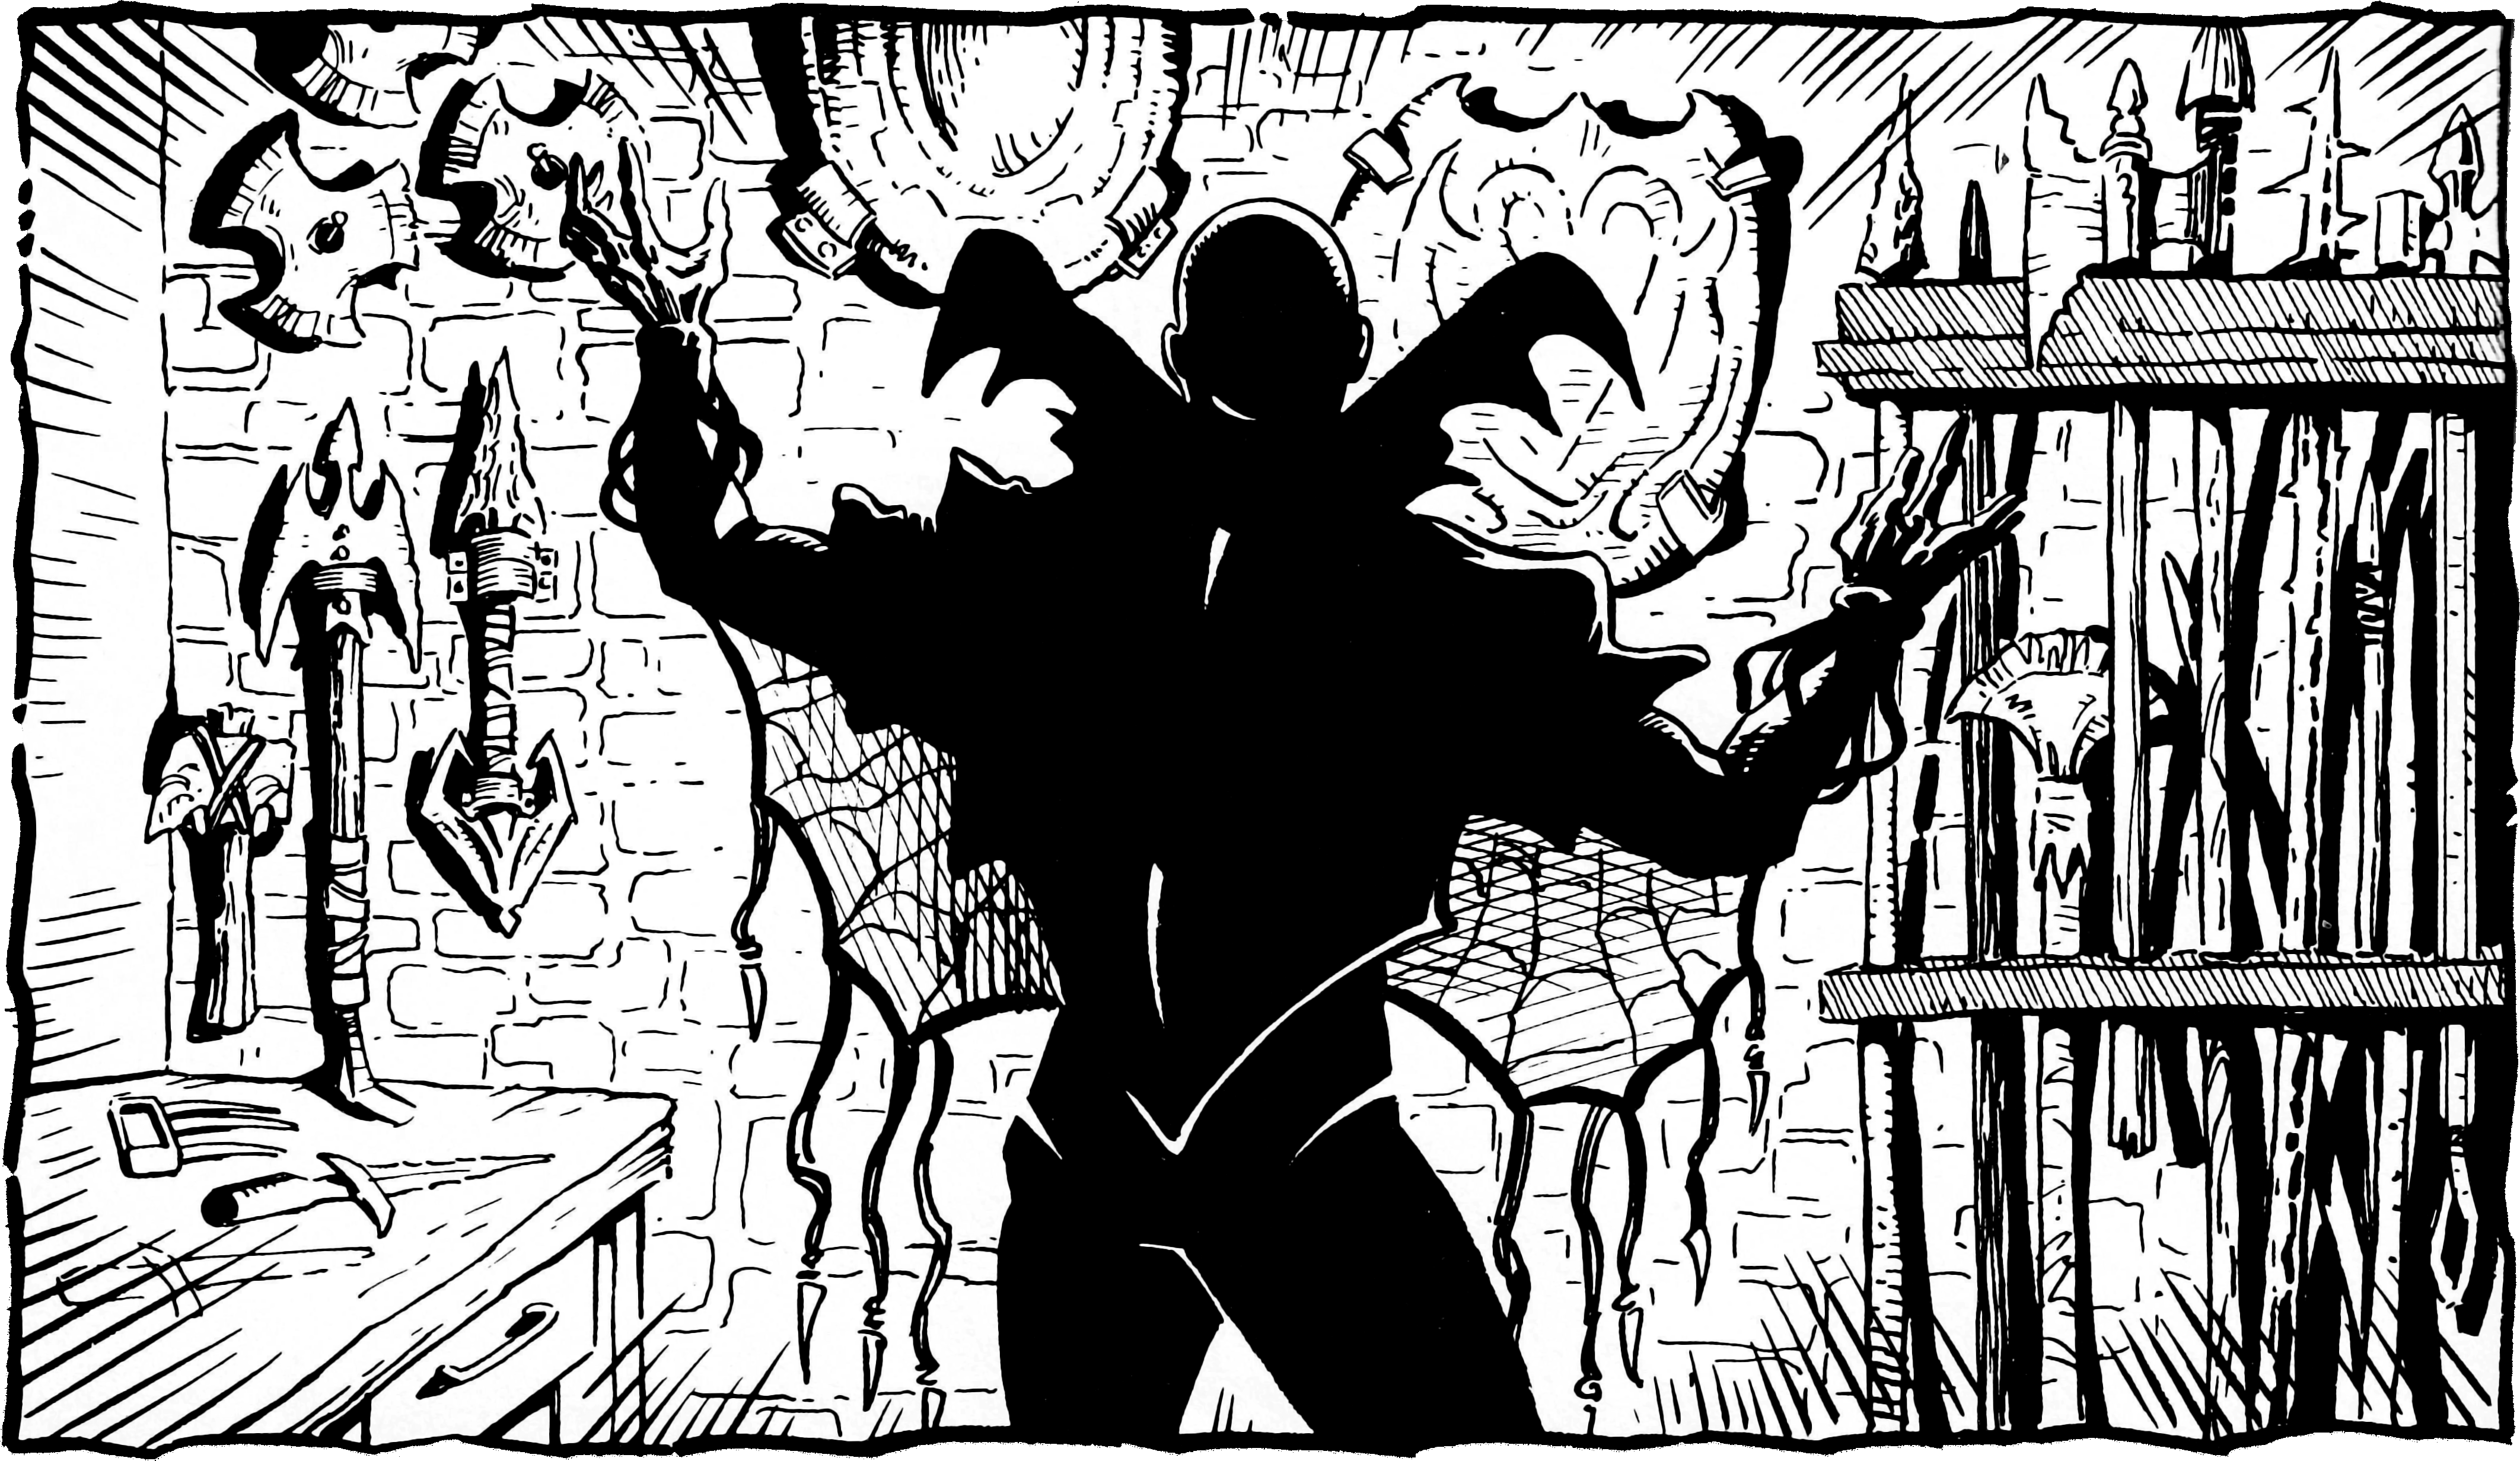
\includegraphics[width=\textwidth-1cm]{images/weapons-1.png}
\WOTC
\end{figure*}

\section{Handling Magic Items}

\subsection{Identifying Items}
\textbf{Trial and Error:} Close study of an item might provide some information. A DC 15 (or maybe 20) \skill{Search} check should reveal a clue for how the item works, such as a tiny command word etched inside a ring or feather motifs that hint the ability to fly.

You might also permit a character to attempt a DC 30 \skill{Spellcraft} check or \skill{Knowledge} (arcana) check to determine if she can attune herself with the item's power or if she remembers reading of it once in her studies.

\textbf{Spells:} The easiest way to discern whether an object is magical is to use \spell{detect magic}. A character can focus on an item to determine the school of the spells embedded within it and the strength of the aura it gives off. The \spell{identify} and \spell{analyze dweomer} spells provide much more information.

\subsubsection{Magic Items and \emph{Detect Magic}}
When \spell{detect magic} identifies a magic item's school of magic, this information refers to the school of the spell placed within the potion, scroll, or wand, or the prerequisite given for the item. The description of each item provides its aura strength and the school it belongs to.

If more than one spell is given as a prerequisite, use the highest-level spell. If no spells are included in the prerequisites, use the following default guidelines.

\Table{}{lX}{
\tableheader Item Nature & \tableheader School \\
Armor and protection items & Abjuration \\
Weapons or offensive items & Evocation \\
Bonus to ability score, on skill check, etc. & Transmutation \\
}

\subsection{Using Items}
To use a magic item, it must be activated, although sometimes activation simply means putting a ring on your finger. Some items, once donned, function constantly. In most cases, using an item requires a standard action that does not provoke attacks of opportunity. By contrast, spell completion items are treated like spells in combat and do provoke attacks of opportunity.

Activating a magic item is a standard action unless the item description indicates otherwise. However, the casting time of a spell is the time required to activate the same power in an item, regardless of the type of magic item, unless the item description specifically states otherwise.

The four ways to activate magic items are described below.

\textbf{Spell Completion:} This is the activation method for scrolls. A scroll is a spell that is mostly finished. The preparation is done for the caster, so no preparation time is needed beforehand as with normal spellcasting. All that's left to do is perform the finishing parts of the spellcasting (the final gestures, words, and so on). To use a spell completion item safely, a character must be of high enough level in the right class to cast the spell already. If he can't already cast the spell, there's a chance he'll make a mistake. Activating a spell completion item is a standard action and provokes attacks of opportunity exactly as casting a spell does.

\textbf{Spell Trigger:} Spell trigger activation is similar to spell completion, but it's even simpler. No gestures or spell finishing is needed, just a special knowledge of spellcasting that an appropriate character would know, and a single word that must be spoken. Anyone with a spell on his or her spell list knows how to use a spell trigger item that stores that spell. (This is the case even for a character who can't actually cast spells, such as a 3rd-level ranger.) The user must still determine what spell is stored in the item before she can activate it. Activating a spell trigger item is a standard action and does not provoke attacks of opportunity.

\textbf{Command Word:} If no activation method is suggested either in the magic item description or by the nature of the item, assume that a command word is needed to activate it. Command word activation means that a character speaks the word and the item activates. No other special knowledge is needed.

A command word can be a real word, but when this is the case, the holder of the item runs the risk of activating the item accidentally by speaking the word in normal conversation. More often, the command word is some seemingly nonsensical word, or a word or phrase from an ancient language no longer in common use. Activating a command word magic item is a standard action and does not provoke attacks of opportunity. 

Sometimes the command word to activate an item is written right on the item. Occasionally, it might be hidden within a pattern or design engraved on, carved into, or built into the item, or the item might bear a clue to the command word.

The \skill{Knowledge} (arcana) and \skill{Knowledge} (history) skills might be useful in helping to identify command words or deciphering clues regarding them. A successful check against DC 30 is needed to come up with the word itself. If that check is failed, succeeding on a second check (DC 25) might provide some insight into a clue.

The spells \spell{identify} and \spell{analyze dweomer} both reveal command words.

\textbf{Use-Activated:} This type of item simply has to be used in order to activate it. A character has to drink a potion, swing a sword, interpose a shield to deflect a blow in combat, look through a lens, sprinkle dust, wear a ring, or don a hat. Use activation is generally straightforward and self-explanatory.

Many use-activated items are objects that a character wears. Continually functioning items are practically always items that one wears. A few must simply be in the character's possession (on his person). However, some items made for wearing must still be activated. Although this activation sometimes requires a command word, usually it means mentally willing the activation to happen. The description of an item states whether a command word is needed in such a case.

Unless stated otherwise, activating a use-activated magic item is either a standard action or not an action at all and does not provoke attacks of opportunity, unless the use involves performing an action that provokes an attack of opportunity in itself. If the use of the item takes time before a magical effect occurs, then use activation is a standard action. If the item's activation is subsumed in its use and takes no extra time use activation is not an action at all.

Use activation doesn't mean that if you use an item, you automatically know what it can do. You must know (or at least guess) what the item can do and then use the item in order to activate it, unless the benefit of the item comes automatically, such from drinking a potion or swinging a sword.
\subsection{Size And Magic Items}
When an article of magic clothing or jewelry is discovered, most of the time size shouldn't be an issue. Many magic garments are made to be easily adjustable, or they adjust themselves magically to the wearer. Size should not keep characters of various kinds from using magic items.

There may be rare exceptions, especially with racial specific items.

\textbf{Armor and Weapon Sizes:} Armor and weapons that are found at random have a 30\% chance of being Small (01--30), a 60\% chance of being Medium (31--90), and a 10\% chance of being any other size (91--100). 
\subsection{Magic Items On The Body}
Many magic items need to be donned by a character who wants to employ them or benefit from their abilities. It's possible for a creature with a humanoid-shaped body to wear as many as twelve magic items at the same time. However, each of those items must be worn on (or over) a particular part of the body.

A humanoid-shaped body can be decked out in magic gear consisting of one item from each of the following groups, keyed to which place on the body the item is worn.

\begin{itemize*}
\item One headband, hat, helmet, or phylactery on the head
\item One pair of eye lenses or goggles on or over the eyes
\item One amulet, brooch, medallion, necklace, periapt, or scarab around the neck
\item One vest, vestment, or shirt on the torso
\item One robe or suit of armor on the body (over a vest, vestment, or shirt)
\item One belt around the waist (over a robe or suit of armor)
\item One cloak, cape, or mantle around the shoulders (over a robe or suit of armor)
\item One pair of bracers or bracelets on the arms or wrists
\item One glove, pair of gloves, or pair of gauntlets on the hands
\item One ring on each hand (or two rings on one hand)
\item One pair of boots or shoes on the feet
\end{itemize*}

Of course, a character may carry or possess as many items of the same type as he wishes. However, additional items beyond those listed above have no effect.

Some items can be worn or carried without taking up space on a character's body. The description of an item indicates when an item has this property. 

\subsection{Saving Throws Against Magic Item Powers}
Magic items produce spells or spell-like effects. For a saving throw against a spell or spell-like effect from a magic item, the DC is 10 + the level of the spell or effect + the ability modifier of the minimum ability score needed to cast that level of spell.

Staffs are an exception to the rule. Treat the saving throw as if the wielder cast the spell, including caster level and all modifiers to save DC.

Most item descriptions give saving throw DCs for various effects, particularly when the effect has no exact spell equivalent (making its level otherwise difficult to determine quickly).

\subsection{Damaging Magic Items}
A magic item doesn't need to make a saving throw unless it is unattended, it is specifically targeted by the effect, or its wielder rolls a natural 1 on his save. Magic items should always get a saving throw against spells that might deal damage to them---even against attacks from which a nonmagical item would normally get no chance to save. Magic items use the same saving throw bonus for all saves, no matter what the type (Fortitude, Reflex, or Will). A magic item's saving throw bonus equals 2 + \onehalf its caster level (round down). The only exceptions to this are intelligent magic items, which make Will saves based on their own Wisdom scores.

Magic items, unless otherwise noted, take damage as nonmagical items of the same sort. A damaged magic item continues to function, but if it is destroyed, all its magical power is lost.

\subsection{Repairing Magic Items}
Some magic items take damage over the course of an adventure. It costs no more to repair a magic item with the Craft skill than it does to repair its nonmagical counterpart. The make whole spell also repairs a damaged---but not completely broken---magic item.

\subsection{Intelligent Items}
Some magic items, particularly weapons, have an intelligence all their own. Only permanent magic items (as opposed to those with a single use or those with charges) can be intelligent. (This means that potions, scrolls, and wands, among other items, are never intelligent.)

In general, less than 1\% of magic items have intelligence.

\subsection{Cursed Items}
Some items are cursed---incorrectly made, or corrupted by outside forces. Cursed items might be particularly dangerous to the user, or they might be normal items with a minor flaw, an inconvenient requirement, or an unpredictable nature. Randomly generated items are cursed 5\% of the time.

\subsection{Charges, Doses, And Multiple Uses}
Many items, particularly wands and staffs, are limited in power by the number of charges they hold. Normally, charged items have 50 charges at most. If such an item is found as a random part of a treasure, roll d\% and divide by 2 to determine the number of charges left (round down, minimum 1). If the item has a maximum number of charges other than 50, roll randomly to determine how many charges are left.

Prices listed are always for fully charged items. (When an item is created, it is fully charged.) For an item that's worthless when its charges run out (which is the case for almost all charged items), the value of the partially used item is proportional to the number of charges left. For an item that has usefulness in addition to its charges, only part of the item's value is based on the number of charges left.

\section{Magic Item Descriptions}
Each general type of magic item gets an overall description, followed by descriptions of specific items.

General descriptions include notes on activation, random generation, and other material. The AC, hardness, hit points, and break DC are given for typical examples of some magic items. The AC assumes that the item is unattended and includes a $-5$ penalty for the item's effective Dexterity of 0. If a creature holds the item, use the creature's Dexterity modifier in place of the $-5$ penalty.

Some individual items, notably those that simply store spells and nothing else, don't get full-blown descriptions. Reference the spell's description for details, modified by the form of the item (potion, scroll, wand, and so on). Assume that the spell is cast at the minimum level required to cast it.

Items with full descriptions have their powers detailed, and each of the following topics is covered in notational form at the end of the description.

\textbf{Aura:} Most of the time, a detect magic spell will reveal the school of magic associated with a magic item and the strength of the aura an item emits. This information (when applicable) is given at the beginning of the item's notational entry. See the detect magic spell description for details.

\textbf{Caster Level:} The next item in a notational entry gives the caster level of the item, indicating its relative power. The caster level determines the item's saving throw bonus, as well as range or other level-dependent aspects of the powers of the item (if variable). It also determines the level that must be contended with should the item come under the effect of a dispel magic spell or similar situation. This information is given in the form ``CL x,'' where ``CL'' is an abbreviation for caster level and ``x'' is an ordinal number representing the caster level itself.

For potions, scrolls, and wands, the creator can set the caster level of an item at any number high enough to cast the stored spell and not higher than her own caster level. For other magic items, the caster level is determined by the creator. The minimum caster level is that which is needed to meet the prerequisites given.

\textbf{Prerequisites:} Certain requirements must be met in order for a character to create a magic item. These include feats, spells, and miscellaneous requirements such as level, alignment, and race or kind. The prerequisites for creation of an item are given immediately following the item's caster level.

A spell prerequisite may be provided by a character who has prepared the spell (or who knows the spell, in the case of a sorcerer or bard), or through the use of a spell completion or spell trigger magic item or a spell-like ability that produces the desired spell effect. For each day that passes in the creation process, the creator must expend one spell completion item or one charge from a spell trigger item if either of those objects is used to supply a prerequisite.

It is possible for more than one character to cooperate in the creation of an item, with each participant providing one or more of the prerequisites. In some cases, cooperation may even be necessary.

If two or more characters cooperate to create an item, they must agree among themselves who will be considered the creator for the purpose of determinations where the creator's level must be known. The character designated as the creator pays the XP required to make the item.

Typically, a list of prerequisites includes one feat and one or more spells (or some other requirement in addition to the feat).

When two spells at the end of a list are separated by ``or,'' one of those spells is required in addition to every other spell mentioned prior to the last two.

\textbf{Market Price:} This gold piece value, given following the word ``Price,'' represents the price someone should expect to pay to buy the item. The market price for an item that can be constructed with an item creation feat is usually equal to the base price plus the price for any components (material or XP).

\textbf{Cost to Create:} The next part of a notational entry is the cost in cp and XP to create the item, given following the word ``Cost.'' This information appears only for items with components (material or XP), which make their market prices higher than their base prices. The cost to create includes the costs derived from the base cost plus the costs of the components.

Items without components do not have a ``Cost'' entry. For them, the market price and the base price are the same. The cost in cp is \onehalf the market price, and the cost in XP is 1/25 the market price.

\textbf{Weight:} The notational entry for many wondrous items ends with a value for the item's weight. When a weight figure is not given, the item has no weight worth noting (for purposes of determining how much of a load a character can carry). 

\subsectionA{Armors}
In general, magic armor protects the wearer to a greater extent than nonmagical armor. Magic armor bonuses are enhancement bonuses, never rise above +5, and stack with regular armor bonuses (and with shield and magic shield enhancement bonuses). All magic armor is also masterwork armor, reducing armor check penalties by 1.

In addition to an enhancement bonus, armor may have special abilities. Special abilities usually count as additional bonuses for determining the market value of an item, but do not improve AC. A suit of armor cannot have an effective bonus (enhancement plus special ability bonus equivalents) higher than +10. A suit of armor with a special ability must have at least a +1 enhancement bonus.

A suit of armor or a shield may be made of an unusual material. Roll d\%: 01--95 indicates that the item is of a standard sort, and 96--100 indicates that it is made of a special material.

Armor is always created so that even if the type of armor comes with boots or gauntlets, these pieces can be switched for other magic boots or gauntlets.

\textbf{Caster Level for Armor and Shields:} The caster level of a magic shield or magic armor with a special ability is given in the item description. For an item with only an enhancement bonus, the caster level is three times the enhancement bonus. If an item has both an enhancement bonus and a special ability, the higher of the two caster level requirements must be met.

\textbf{Shields:} Shield enhancement bonuses stack with armor enhancement bonuses. Shield enhancement bonuses do not act as attack or damage bonuses when the shield is used in a bash. The bashing special ability, however, does grant a +1 bonus on attack and damage rolls.

A shield could be built that also acted as a magic weapon, but the cost of the enhancement bonus on attack rolls would need to be added into the cost of the shield and its enhancement bonus to AC.

As with armor, special abilities built into the shield add to the market value in the form of additions to the bonus of the shield, although they do not improve AC. A shield cannot have an effective bonus (enhancement plus special ability bonus equivalents) higher than +10. A shield with a special ability must have at least a +1 enhancement bonus.

\textbf{Shield Hardness and Hit Points:} Each +1 of enhancement bonus adds 2 to a shield's hardness and +10 to its hit points.

\textbf{Activation:} Usually a character benefits from magic armor and shields in exactly the way a character benefits from nonmagical armor and shields---by wearing them. If armor or a shield has a special ability that the user needs to activate then the user usually needs to utter the command word (a standard action).

\textbf{Armor for Unusual Creatures:} The cost of armor for nonhumanoid creatures, as well as for creatures who are neither Small nor Medium, varies. The cost of the masterwork quality and any magical enhancement remains the same.

\Table{Armor and Shield Enhancements}{CR}{
\tableheader Armor Bonus & \tableheader Base Price\\
+1 & 1,000 cp\\
+2 & 4,000 cp\\
+3 & 9,000 cp\\
+4 & 16,000 cp\\
+5 & 25,000 cp\\
+6\footnotemark[1] & 36,000 cp\\
+7\footnotemark[1] & 49,000 cp\\
+8\footnotemark[1] & 64,000 cp\\
+9\footnotemark[1] & 81,000 cp\\
+10\footnotemark[1] & 100,000 cp\\
\TableNote{2}{1 Armor and shields can't actually have bonuses this high. Use these lines to determine price when special abilities are added in.}
}

\subsubsection{Magic Armor and Shield Special Ability Descriptions}
Most magic armor and shields only have enhancement bonuses. Such items can also have one or more of the special abilities detailed below. Armor or a shield with a special ability must have at least a +1 enhancement bonus.

\Table{Armor Special Abilities}{lR}{
\tableheader Special Ability & \tableheader Base Price Modifier\\
Glamered & +2,700 cp \\
Fortification, light & +1 bonus \\
Quickness & +1 bonus \\
Shade & +1 bonus \\
Shadow & +3,750 cp \\
Silent moves & +3,750 cp \\
Slick & +3,750 cp \\
Invulnerability & +4,000 cp \\
Landing & +5,000 cp \\
Lifewall & +6,000 cp \\
% Linked & +2 bonus \\
Spell resistance (13) & +2 bonus \\
Malleable & +10,800 cp \\
Shadow, improved & +15,000 cp \\
Silent moves, improved & +15,000 cp \\
Slick, improved & +15,000 cp \\
Acid resistance & +18,000 cp \\
Cold resistance & +18,000 cp \\
Eletric resistance & +18,000 cp \\
Fire resistance & +18,000 cp \\
Sonic resistance & +18,000 cp \\
% Mindarmor & +24,000 cp \\
Fortification, moderate & +3 bonus \\
Ghost touch & +3 bonus \\
Gleaming & +3 bonus \\
Spell resistance (15) & +3 bonus \\
% Vanishing & +3 bonus \\
Wild & +3 bonus \\
Psychic & +30,000 cp \\
Shadow, greater & +33,750 cp \\
Silent moves, greater & +33,750 cp \\
Slick, greater & +33,750 cp \\
Acid resistance, improved & +42,000 cp \\
Cold resistance, improved & +42,000 cp \\
Eletric resistance, improved & +42,000 cp \\
Fire resistance, improved & +42,000 cp \\
Sonic resistance, improved & +42,000 cp \\
Spell resistance (17) & +4 bonus \\
Etherealness & +49,000 cp \\
Undead controlling & +49,000 cp \\
Fortification, heavy & +5 bonus \\
Spell resistance (19) & +5 bonus \\
Phasing & +65,520 cp \\
Acid resistance, greater & +66,000 cp \\
Cold resistance, greater & +66,000 cp \\
Eletric resistance, greater & +66,000 cp \\
Fire resistance, greater & +66,000 cp \\
Sonic resistance, greater & +66,000 cp \\
}

\Table{Shield Special Abilities}{lR}{
\tableheader Special Ability & \tableheader Base Price Modifier\\
Arrow Catching & +1 bonus \\
Bashing & +1 bonus \\
Blinding & +1 bonus \\
% Linked & +6,000 cp \\
Animated & +2 bonus \\
Arrow Deflection & +2 bonus \\
Manifester & +10,800 cp\\
% Mindarmor & +24,000 cp\\
Ghost Touch & +3 bonus \\
% Vanishing & +3 bonus \\
Wild & +3 bonus \\
Undead Controlling & +49,000 cp \\
Reflecting & +5 bonus \\
% Time Buttress & +5 bonus \\
}

\textbf{Animated:} Upon command, an animated shield floats within 60 centimeters of the wielder, protecting her as if she were using it herself but freeing up both her hands. Only one shield can protect a character at a time. A character with an animated shield still takes any penalties associated with shield use, such as armor check penalty, arcane spell failure chance, and nonproficiency.

Strong transmutation; CL 12th; \feat{Craft Magic Arms and Armor}, \spell{animate objects}; Price +2 bonus.

\textbf{Arrow Catching:} A shield with this ability attracts ranged weapons to it. It has a deflection bonus of +1 against ranged weapons because projectiles and thrown weapons veer toward it. Additionally, any projectile or thrown weapon aimed at a target within 1.5 meter of the shield's wearer diverts from its original target and targets the shield's bearer instead. (If the wielder has total cover relative to the attacker, the projectile or thrown weapon is not diverted.) Additionally, those attacking the wearer with ranged weapons ignore any miss chances that would normally apply. Projectiles and thrown weapons that have an enhancement bonus higher than the shield's base AC bonus are not diverted to the wearer (but the shield's increased AC bonus still applies against these weapons). The wielder can activate or deactivate this ability with a command word.

Moderate abjuration; CL 8th; \feat{Craft Magic Arms and Armor}, \spell{entropic shield}; Price +1 bonus.

\textbf{Arrow Deflection:} A shield with this ability protects the wielder from ranged attacks. Once per round when he would normally be struck by a ranged weapon, he can make a DC 20 Reflex save. If the ranged weapon has an enhancement bonus, the DC increases by that amount. If he succeeds, the shield deflects the weapon. He must be aware of the attack and not flat-footed. Attempting to deflect a ranged weapon doesn't count as an action. Exceptional ranged weapons, such as boulders hurled by giants or acid arrows, can't be deflected.

Faint abjuration; CL 5th; \feat{Craft Magic Arms and Armor}, \spell{shield}; Price +2 bonus.

\textbf{Bashing:} A shield with this special ability is designed to perform a shield bash. A bashing shield deals damage as if it were a weapon of two size categories larger (a Medium light shield thus deals 1d6 points of damage and a Medium heavy shield deals 1d8 points of damage). The shield acts as a +1 weapon when used to bash. (Only light and heavy shields can have this ability.)

Moderate transmutation; CL 8th; \feat{Craft Magic Arms and Armor}, \spell{bull's strength}; Price +1 bonus.

\textbf{Blinding:} A shield with this ability flashes with a brilliant light up to twice per day upon command of the wielder. Anyone within 6 meters except the wielder must make a DC 14 Reflex save or be blinded for 1d4 rounds.

Moderate evocation; CL 7th; \feat{Craft Magic Arms and Armor}, \spell{searing light}; Price +1 bonus. 

\textbf{Energy Resistance:} This armor absorbs the first points of one specific type of energy damage per attack that the wearer would normally take (similar to the \spell{resist energy} spell). Each type of energy has a different visual:

\textit{Acid Resistance:} A suit of armor or a shield with this property normally has a dull gray appearance.

\textit{Cold Resistance:} A suit of armor or a shield with this property normally has a bluish, icy hue or is adorned with furs and shaggy pelts.

\textit{Eletric Resistance:} A suit of armor or a shield with this property normally has a bluish hue and often bears a storm or lightning motif.

\textit{Fire Resistance:} A suit of armor with this ability normally has a reddish hue and often is decorated with a draconic motif.

\textit{Sonic Resistance:} A suit of armor or a shield with this property normally has a glistening appearance.

\Table{}{XCr{22mm}}{
\tableheader Strength & \tableheader Energy Resistance & \tableheader Base Price Modifier\\
Normal & 10 & +18,000 cp \\
Improved & 20 & +42,000 cp \\
Greater & 30 & +66,000 cp \\
}

Faint abjuration (light), or moderate abjuration (improved or greater); CL 3rd (light), 7th (improved), or 11th (greater); \feat{Craft Magic Arms and Armor}, \spell{resist energy}; Price varies (see above).

\textbf{Etherealness:} On command, this ability allows the wearer of the armor to become ethereal (as the \spell{ethereal jaunt} spell) once per day. The character can remain ethereal for as long as desired, but once he returns to normal, he cannot become ethereal again that day.

Strong transmutation; CL 13th; \feat{Craft Magic Arms and Armor}, \spell{ethereal jaunt}; Price +49,000 cp. 

\textbf{Fortification:} This suit of armor or shield produces a magical force that protects vital areas of the wearer more effectively. When a critical hit or sneak attack is scored on the wearer, there is a chance that the critical hit or sneak attack is negated and damage is instead rolled normally.

\Table{}{lCr{22mm}}{
\tableheader Fortification Type & \tableheader Chance for Normal Damage & \tableheader Base Price Modifier \\
Light & 25\% & +1 bonus\\
Moderate & 75\% & +3 bonus\\
Heavy & 100\% & +5 bonus\\
}

Strong abjuration; CL 13th; \feat{Craft Magic Arms and Armor}, \spell{limited wish} or \spell{miracle}; Price varies (see above).

\textbf{Ghost Touch:} This armor or shield seems almost translucent. Both its enhancement bonus and its armor bonus count against the attacks of incorporeal creatures. It can be picked up, moved, and worn by incorporeal creatures at any time. Incorporeal creatures gain the armor or shield's enhancement bonus against both corporeal and incorporeal attacks, and they can still pass freely through solid objects.

Strong transmutation; CL 15th; \feat{Craft Magic Arms and Armor}, \spell{etherealness}; Price +3 bonus.

\textbf{Glamered:} A suit of armor with this ability appears normal. Upon command, the armor changes shape and form to assume the appearance of a normal set of clothing. The armor retains all its properties (including weight) when glamered. Only a \spell{true seeing} spell or similar magic reveals the true nature of the armor when disguised.

Moderate illusion; CL 10th; \feat{Craft Magic Arms and Armor}, \spell{disguise self}; Price +2,700 cp.

\textbf{Gleaming:} Gleams and flashes from the armor give the wearer and his armor a ``fuzzy'' appearance, granting the wearer concealment.

Faint illusion; CL 5th; \feat{Craft Magic Arms and Armor}, \spell{blur}; Price +3 bonus.

\textbf{Invulnerability:} This suit of armor grants the wearer damage reduction of 5/magic.

Strong abjuration and perhaps evocation (if \spell{miracle} is used); CL 18th; \feat{Craft Magic Arms and Armor}, \spell{stoneskin}, \spell{wish} or \spell{miracle}; Price +3 bonus.

\textbf{Landing:} A suit of armor with this capability allows the wearer to ignore any damage dealt by the first 18 meters of a fall. Regardless of the height of a fall, the wearer always lands on her feet.

Faint transmutation; CL 4th; \feat{Craft Magic Arms and Armor}, \spell{feather fall}; Price +4,000 cp.

\textbf{Lifewall:} This suit of armor protects the wearer from the effects of being caught in the defiling radius of a spellcasting defiler. The wearer is immune to all penalties and damage associated with the defiling radius, even when augmented with raze feats or magical items.

Moderate abjuration; CL 11th; \feat{Craft Magic Arms and Armor}, \spell{allegiance of the land}; Price +5,000 cp.

% \textbf{Linked:} This kind of armor or shield allows the wearer to form a telepathic bond with other wearers of linked armor or shields within 15 kilometers. This ability is otherwise similar to the \psionic{mindlink} power.

% Moderate divination; CL 6th; \feat{Craft Magic Arms and Armor}, \psionic{mindlink}; Price +6,000 cp.

\textbf{Malleable:} Malleable armor seems thinner, lighter, and a little more flexible than its mundane counterpart. Spell failure chances for malleable armor are decreased by 10\%, the maximum Dexterity bonus is increased by 2, and armor check penalties are lessened by 3 (to a minimum of 0). If the armor is medium or heavy armor, it is treated as light armor for all purposes, such as when sleeping in armor or when determining the character's movement speed.

Faint transmutation; CL 5th; \feat{Craft Magic Arms and Armor}, \spell{gaseous form}; Price +2 bonus.

\textbf{Manifester:} This kind of shield generates 3 power points once per day that the wearer can use when manifesting a power he knows. These power points must all be used on the same power. As usual, a psionic character cannot pay a power's cost with power points from more than one source, so the power points in the shield must be used for discrete manifestations.

Moderate transmutation; CL 7th; \feat{Craft Magic Arms and Armor}, \spell{dweomer of transference}, knowledge of any 2nd-level psionic power; Price +10,800 cp.

% \textbf{Mindarmor:} This kind of armor or shield grants the wearer a +3 insight bonus on Will saving throws to resist all mind-affecting and/or compulsion powers.

% Faint abjuration; CL 5th; \feat{Craft Magic Arms and Armor}, \psionic{empty mind}; Price +24,000 cp.

\textbf{Phasing:} The wearer of this kind of armor can move through wooden, plaster, or stone walls, but not other materials. The wearer can call on this special ability as a standard action. When the phasing ability is active, the wearer can pass through a wall or some other kind of appropriate object for a total distance of 18 meters per day (see below), breaking this distance up into several smaller passages or one long one, as desired. A wearer who exceeds this daily distance limit while inside solid material is ejected from the material at the point of entry, ending up prone in front of the now impassable barrier.

Phasing through a wall that separates two adjacent squares on the grid counts as 1.5 meter of distance. Phasing through a wall or barrier of any greater thickness counts as a distance equal to the barrier's thickness plus 1.5 meter.

Strong conjuration; CL 13th; \feat{Craft Magic Arms and Armor}, \spell{phase door}; Price +65,520 cp.

\textbf{Psychic:} A psychic armor's power depends on its wearer. When worn by a nonpsionic creature, the armor possesses the qualities of a nonmagical, nonpsionic suit of masterwork armor. When worn by a psionic creature, this armor has an enhancement bonus based on the wearer's current power points reserve, as shown on the following table. The armor's enhancement bonus decreases as the wearer spends power points, and it increases whenever the wearer gains enough power points (by any means) to put his power points reserve into the next higher category.

\Table{}{r{1cm}lClr{1cm}}{
& \tableheader Power Point Reserve & \tableheader Enhancement Bonus & \\
& 1--4 & +1 & \\
& 5--29 & +2 & \\
& 30--79 & +3 & \\
& 80--129 & +4 & \\
& 130 or higher & +5 & \\
}

Strong abjuration; CL 17th; \feat{Craft Magic Arms and Armor}, \spell{dweomer of transference}, \spell{wish} or \spell{miracle}, must have a power point reserve; Price +30,000 cp.

\textbf{Quickness:} This kind of armor increases the wearer's speed by 1.5 meter. Thus, a character whose normal speed in armor is 6 meters moves 7.5 meters in \emph{armor of quickness}.

Faint transmutation; CL 4th; \feat{Craft Magic Arms and Armor}, \spell{expeditious retreat} or \psionic{burst}; Price +1 bonus.

\textbf{Reflecting:} This shield seems like a mirror. Its surface is completely reflective. Once per day, it can be called on to reflect a spell back at its caster exactly like the \spell{spell turning} spell.

Strong abjuration; CL 14th; \feat{Craft Magic Arms and Armor}, \spell{spell turning}; Price +5 bonus. 

\textbf{Shade:} Armor made with this ability is very beneficial to their wearer's when under the Athasian sun. The wearer is considered to be in shade for all purposes, and only require half their normal water intake to prevent dehydration. The wearer is not considered to be wearing armor for the purpose of Fortitude saves dealt by heat exposure from the environment.

Faint conjuration; CL 1st, \feat{Craft Magical Arms and Armor}, \spell{cooling canopy}; Price +1 bonus.

\textbf{Shadow:} This armor is jet black and blurs the wearer whenever she tries to hide, granting a competence bonus on \skill{Hide} checks. (The armor's armor check penalty still applies normally.)

\Table{}{XCr{22mm}}{
\tableheader Strength & \tableheader \skill{Hide} bonus & \tableheader Base Price Modifier\\
Normal & +5 & +3,750 cp \\
Improved & +10 & +15,000 cp \\
Greater & +20 & +33,750 cp \\
}

Faint illusion (light), moderate illusion (improved or greater); CL 5th (light), 10th (improved), 15th (greater); \feat{Craft Magic Arms and Armor}, \spell{invisibility}; Price varies (see above).

\textbf{Silent Moves:} This armor is well oiled and magically constructed so that it not only makes little sound, but it dampens sound around it. It provides a competence bonus on its wearer's \skill{Move Silently} checks. (The armor's armor check penalty still applies normally.)

\Table{}{XCr{22mm}}{
\tableheader Strength & \tableheader \skill{Move Silently} bonus & \tableheader Base Price Modifier\\
Normal & +5 & +3,750 cp \\
Improved & +10 & +15,000 cp \\
Greater & +20 & +33,750 cp \\
}

Faint illusion (light), moderate illusion (improved or greater); CL 5th (light), 10th (improved), 15th (greater); \feat{Craft Magic Arms and Armor}, \spell{silence}; Price varies (see above).

\textbf{Slick:} Slick armor seems coated at all times with a slightly greasy oil. It provides a competence bonus on its wearer's \skill{Escape Artist} checks. (The armor's armor check penalty still applies normally.)

\Table{}{XCr{22mm}}{
\tableheader Strength & \tableheader \skill{Escape Artist} bonus & \tableheader Base Price Modifier\\
Normal & +5 & +3,750 cp \\
Improved & +10 & +15,000 cp \\
Greater & +20 & +33,750 cp \\
}

Faint conjuration (light), moderate conjuration (improved or greater); CL 5th (light), 10th (improved), 15th (greater); \feat{Craft Magic Arms and Armor}, \spell{grease}; Price varies (see above).

\textbf{Spell Resistance:} This property grants the armor's wearer spell resistance while the armor is worn. The spell resistance can be 13, 15, 17, or 19, depending on the armor.

Strong abjuration; CL 15th; \feat{Craft Magic Arms and Armor}, \spell{spell resistance}; Price +2 bonus (SR 13), +3 bonus (SR 15), +4 bonus (SR 17), or +5 bonus (SR 19).

% \textbf{Time Buttress:} This kind of shield gives the wielder a chance to avoid telling blows by using time itself as a shield. Once per day, the wielder can use \psionic{timeless body} as though manifesting the power.

% Strong transmutation; CL 17th; \feat{Craft Magic Arms and Armor}, \psionic{timeless body}; Price +5 bonus.

\textbf{Undead Controlling:} The wearer of a suit of armor or a shield with this property may control up to 26 HD of undead per day, as the control undead spell. At dawn each day, the wearer loses control of any undead still under his sway. Armor or a shield with this ability appears to be made of bone; this feature is entirely decorative and has no other effect on the armor.

Strong necromancy; CL 13th; \feat{Craft Magic Arms and Armor}, \spell{control undead}; Price +49,000 cp.

% \textbf{Vanishing:} On command, this suit of armor or shield renders its wearer and all the wearer's equipment invisible to the minds of others, as if he had manifested the power \psionic{cloud mind}. The wearer can use this ability twice per day.

% Faint enchantment; CL 5th; \feat{Craft Magic Arms and Armor}, \psionic{cloud mind}; Price +3 bonus.

\textbf{Wild:} The wearer of a suit of armor or a shield with this ability preserves his armor bonus (and any enhancement bonus) while in a wild shape. Armor and shields with this ability usually appear to be made covered in leaf patterns. While the wearer is in a wild shape, the armor cannot be seen.

Moderate transmutation; CL 9th; \feat{Craft Magic Arms and Armor}, \spell{baleful polymorph}; Price +3 bonus. 
\Table{Specific Armors}{LR}{
  \tableheader Armor
& \tableheader Price \\
Drakehide Plate        & 3,300 cp \\
Banded Mail of Luck    & 18,900 cp \\
Breastplate of Command & 25,400 cp \\
De'utko Armor          & 87,250 cp \\
Adamantine Breastplate & 10,002 gp \\
Dwarven Plate          & 15,015 gp \\
}

\subsubsection{Specific Armors}
The following specific suits of armor usually are preconstructed with exactly the qualities described here.

\textbf{Adamantine Breastplate:} This nonmagical breastplate is made of adamantine, giving its wearer damage reduction of 2/--.

No aura (nonmagical); Price 10,002 gp.

\textbf{Banded Mail of Luck:} Ten 100-cp gems adorn this \emph{+3 banded mail}. Once per week, the armor allows its wearer to require that an attack roll made against him be rerolled. He must take whatever consequences come from the second roll. The wearer's player must decide whether to have the attack roll rerolled before damage is rolled.

Strong enchantment; CL 12th; \feat{Craft Magic Arms and Armor}, \spell{bless}; Price 18,900 cp; Cost 10,150 cp + 700 XP.

\textbf{Breastplate of Command:} This finely crafted \emph{+2 breastplate} radiates a powerful aura of magic. When worn, the armor bestows a dignified and commanding aura upon its owner. The wearer gains a +2 competence bonus on all Charisma checks, including turning checks and Charisma-based skill checks. The wearer also gains a +2 competence bonus to his \feat{Leadership} score. Friendly troops within 102 meters of the user become braver than normal. Since the effect arises in great part from the distinctiveness of the armor, the wearer cannot hide or conceal herself in any way and still have the effect function.

Strong enchantment; CL 15th; \feat{Craft Magic Arms and Armor}, \spell{mass charm monster}; Price 25,400 cp; Cost 10,975 cp + 850 XP.

\textbf{De'utko Armor:} This elven suit of armor, whose name means ``sleepless'' in their tongue, is fashioned from the chitinuous shells of slain thri-kreen by the tribe's best artisan. It is etched with markings symbolizing the glory of the hunt and slaying of the hated insect-men. Only kreen slayers don this armor, using its powers to aid in hunting and protecting their tribes for long periods of time without fear of letting their guards down in face of the sleepless mantis warrior.

This \emph{+2 improved silent moves chitin armor} renders the wearer immune to all spells and effects that restrict his movement, as if he were under the effect of a \spell{freedom of movement} spell. He also receives the benefit of the thri-kreen's sleep immunity racial ability for a number of days equal to 7 + his Constitution modifier, after which time 8 hours of uninterrupted sleep are needed before gaining the benefits of this ability again. A spellcasting or manifesting wearer must rest as usual each time he wants to prepare new spells or regain spent power points.

Strong abjuration; CL 17th; \feat{Craft Magic Arms and Armor}, creator must be an elf, \spell{freedom of movement}, \spell{silence}, \spell{wakefulness}; Price 87,250 cp; Cost 53,250 cp + 2,720 XP.

\textbf{Drakehide Plate:} This suit of full plate is made of drakehide, rather than metal, so druids can wear it. It is otherwise identical to masterwork full plate.

No aura (nonmagical); Price 3,300 cp.

\textbf{Dwarven Plate:} This full plate is made of adamantine, giving its wearer damage reduction of 3/--.

No aura (nonmagical); Price 15,015 gp.

\Table{Specific Shields}{LR}{
\tableheader Shield & \tableheader Price \\
Darkwood Buckler & 205 cp \\
Darkwood Shield  & 257 cp \\
Caster's Shield  & 3,153 cp \\
Spined Shield    & 5,580 cp \\
Lion's Shield    & 9,257 cp \\
Winged Shield    & 17,257 cp \\
Absorbing Shield & 50,257 cp \\
}

\subsubsection{Specific Shields}
The following specific shields usually are preconstructed with exactly the qualities described here.


\textbf{Absorbing Shield:} This \emph{+1 heavy darkwood shield} is flat black and seems to absorb light. Once every two days, on command, it can disintegrate an object that it touches, as the spell but requiring a melee touch attack.

Strong transmutation; CL 17th; \feat{Craft Magic Arms and Armor}, \spell{disintegrate}; Price 50,257 cp; Cost 25,257 cp + 2,000 XP.


\textbf{Caster's Shield:} This \emph{+1 light wooden shield} has a small leather strip on the back on which a spellcaster can scribe a single spell as on a scroll. A spell so scribed has only half the base raw material cost. Experience point and component costs remain the same. The strip cannot accommodate spells of higher than 3rd level. The strip is reusable.

A random caster's shield has a 50\% chance of having a single medium scroll spell on it. The spell is divine (01--80 on d\%) or arcane (81--100).

A caster's shield has a 5\% arcane spell failure chance.

Moderate abjuration; CL 6th; \feat{Craft Magic Arms and Armor}, \feat{Scribe Scroll}, creator must be at least 6th level; Price 3,153 cp (plus the value of the scroll spell if one is currently scribed); Cost 1,653 cp + 120 XP.


\textbf{Darkwood Buckler:} This nonmagical light wooden shield is made out of darkwood. It has no enhancement bonus, but its construction material makes it lighter than a normal wooden shield. It weighs 1.25 kilograms and has no armor check penalty.

No aura (nonmagical); Price 205 cp.


\textbf{Darkwood Shield:} This nonmagical heavy wooden shield is made out of darkwood. It has no enhancement bonus, but its construction material makes it lighter than a normal wooden shield. It weighs 2.5 kilograms and has no armor check penalty.

No aura (nonmagical); Price 257 cp.


\textbf{Lion's Shield:} This \emph{+2 heavy darkwood shield} is fashioned to appear to be a roaring lion's head. Three times per day as a free action, the lion's head can be commanded to attack (independently of the shield wearer), biting with the wielder's base attack bonus (including multiple attacks, if the wielder has them) and dealing 2d6 points of damage. This attack is in addition to any actions performed by the wielder.

Moderate conjuration; CL 10th; \feat{Craft Magic Arms and Armor}, \emph{summon nature's ally IV}; Price 9,257 cp; Cost 4,757 cp + 360 XP.


\textbf{Spined Shield:} This \emph{+1 heavy steel shield} is covered in spines. It acts as a normal spiked shield. On command up to three times per day, the shield's wearer can fire one of the shield's spines. A fired spine has a +1 enhancement bonus, a range increment of 36 meters, and deals 1d10 points of damage (19--20/$\times$2). Fired spines regenerate each day.

Moderate evocation; CL 6th; \feat{Craft Magic Arms and Armor}, \emph{magic missile}; Price 5,580 cp; Cost 2,740 cp + 223 XP.


\textbf{Winged Shield:} This round heavy wooden shield has a +3 enhancement bonus. Small, feathered wings encircle the shield.

Once per day it can be commanded to \spell{fly} (as the spell), carrying the wielder. The shield can carry up to 66.5 kilograms and move at 18 meters per round, or up to 133 kilograms and move at 12 meters per round.

Faint transmutation; CL 5th; \feat{Craft Magic Arms and Armor}, \spell{fly}; Price 17,257 cp; Cost 8,628 cp and 5 bits + 690 XP.


\subsectionA{Weapons}
Magic weapons have enhancement bonuses ranging from +1 to +5. They apply these bonuses to both attack and damage rolls when used in combat. All magic weapons are also masterwork weapons, but their masterwork bonus on attack rolls does not stack with their enhancement bonus on attack rolls.

Weapons come in two basic categories: melee and ranged. Some of the weapons listed as melee weapons can also be used as ranged weapons. In this case, their enhancement bonus applies to either type of attack.

In addition to an enhancement bonus, weapons may have special abilities. Special abilities count as additional bonuses for determining the market value of the item, but do not modify attack or damage bonuses (except where specifically noted). A single weapon cannot have a modified bonus (enhancement bonus plus special ability bonus equivalents) higher than +10. A weapon with a special ability must have at least a +1 enhancement bonus.

A weapon or a kind of ammunition may be made of an unusual material. Roll d\%: 01--95 indicates that the item is of a standard sort, and 96--100 indicates that it is made of a special material.

\textbf{Caster Level for Weapons:} The caster level of a weapon with a special ability is given in the item description. For an item with only an enhancement bonus and no other abilities, the caster level is three times the enhancement bonus. If an item has both an enhancement bonus and a special ability, the higher of the two caster level requirements must be met.

\textbf{Additional Damage Dice:} Some magic weapons deal additional dice of damage. Unlike other modifiers to damage, additional dice of damage are not multiplied when the attacker scores a critical hit.

\textbf{Ranged Weapons and Ammunition:} The enhancement bonus from a ranged weapon does not stack with the enhancement bonus from ammunition. Only the higher of the two enhancement bonuses applies.

Ammunition fired from a projectile weapon with an enhancement bonus of +1 or higher is treated as a magic weapon for the purpose of overcoming damage reduction. Similarly, ammunition fired from a projectile weapon with an alignment gains the alignment of that projectile weapon (in addition to any alignment it may already have).

\textbf{Magic Ammunition and Breakage:} When a magic arrow, crossbow bolt, shuriken, or sling bullet misses its target, there is a 50\% chance it breaks or otherwise is rendered useless. A magic arrow, bolt, bullet, or shuriken that hits is destroyed.

\textbf{Light Generation:} Fully 30\% of magic weapons shed light equivalent to a light spell (bright light in a 6-meter radius, shadowy light in a 12-meter radius). These glowing weapons are quite obviously magical. Such a weapon can't be concealed when drawn, nor can its light be shut off. Some of the specific weapons detailed below always or never glow, as defined in their descriptions.

\textbf{Hardness and Hit Points:} Each +1 of enhancement bonus adds 2 to a weapon's or shield's hardness and +10 to its hit points.

\textbf{Activation:} Usually a character benefits from a magic weapon in the same way a character benefits from a mundane weapon---by attacking with it. If a weapon has a special ability that the user needs to activate then the user usually needs to utter a command word (a standard action).

\textbf{Magic Weapons and Critical Hits:} Some weapon qualities and some specific weapons have an extra effect on a critical hit. This special effect functions against creatures not subject to critical hits, such as undead, elementals, and constructs. When fighting against such creatures, roll for critical hits as you would against humanoids or any other creature subject to critical hits. On a successful critical roll, apply the special effect, but do not multiply the weapon's regular damage.

\textbf{Weapons for Unusually Sized Creatures:} The cost of weapons for creatures who are neither Small nor Medium varies. The cost of the masterwork quality and any magical enhancement remains the same.

\textbf{Special Qualities:} Roll d\%. If the item is a melee weapon, a 01--30 result indicates that the item sheds light, 31--45 indicates that something (a design, inscription, or the like) provides a clue to the weapon's function, and 46--100 indicates no special qualities.

If the item is a ranged weapon, a 01--15 result indicates that something (a design, inscription, or the like) provides a clue to the weapon's function, and 16--100 indicates no special qualities.

\Table{Weapon Enhancements}{r{1cm}CRr{1cm}}{
& \tableheader Weapon Bonus & \tableheader Base Price\footnotemark[1] & \\
& +1 & 2,000 cp & \\
& +2 & 8,000 cp & \\
& +3 & 18,000 cp & \\
& +4 & 32,000 cp & \\
& +5 & 50,000 cp & \\
& +6\footnotemark[2] & 72,000 cp & \\
& +7\footnotemark[2] & 98,000 cp & \\
& +8\footnotemark[2] & 128,000 cp & \\
& +9\footnotemark[2] & 162,000 cp & \\
& +10\footnotemark[2] & 200,000 cp & \\
\TableNote{4}{1 This price is for 50 arrows, crossbow bolts, shuriken, or sling bullets.}\\
\TableNote{4}{2 Weapons can't actually have bonuses this high. Use these lines to determine price when special abilities are added in.}\\
}

\subsubsection{Magic Weapon Special Ability Descriptions}
In addition to enhancement bonuses, weapons can have one or more of the special abilities detailed below. A weapon with a special ability must have at least a +1 enhancement bonus.

\Table{Melee Weapon Special Abilities}{lR}{
\tableheader Special Ability & \tableheader Base Price Modifier\\
Bloodlust                        & +1 bonus \\
Chitin-rot                       & +1 bonus \\
Defending                        & +1 bonus \\
Flaming                          & +1 bonus \\
Frost                            & +1 bonus \\
Ghost touch                      & +1 bonus \\
Keen\textsuperscript{1, 2}       & +1 bonus \\
Merciful                         & +1 bonus \\
Mighty cleaving                  & +1 bonus \\
Parching                         & +1 bonus \\
Power storing                    & +1 bonus \\
Returning\footnotemark[3]        & +1 bonus \\
Shock                            & +1 bonus \\
Soul-bleeder                     & +1 bonus \\
Spell storing                    & +1 bonus \\
Thundering                       & +1 bonus \\
Throwing                         & +1 bonus \\
Vicious                          & +1 bonus \\
Anarchic                         & +2 bonus \\
Axiomatic                        & +2 bonus \\
Disruption\footnotemark[4]       & +2 bonus \\
Expiation                        & +2 bonus \\
Flaming burst                    & +2 bonus \\
Holy                             & +2 bonus \\
Icy burst                        & +2 bonus \\
Penetration\footnotemark[2]      & +2 bonus \\
Shattering\textsuperscript{1, 4} & +2 bonus \\
Shocking burst                   & +2 bonus \\
Silencing                        & +2 bonus \\
Unholy                           & +2 bonus \\
Wounding                         & +2 bonus \\
Manifester                       & +16,000 cp \\
Baleful shriek                   & +3 bonus \\
Bodyfeeder                       & +3 bonus \\
Dislocator                       & +3 bonus \\
Doom                             & +3 bonus \\
Rumbling                         & +3 bonus \\
Speed                            & +3 bonus \\
Psychic                          & +35,000 cp \\
Brilliant energy                 & +4 bonus \\
Dancing                          & +4 bonus \\
Great dislocator                 & +4 bonus \\
Malison                          & +4 bonus \\
Cleansing flame                  & +5 bonus \\
Coup de grace                    & +5 bonus \\
Vorpal\footnotemark[1]           & +5 bonus \\
\TableNote{2}{1 Only slashing weapons.}\\
\TableNote{2}{2 Only piercing weapons.}\\
\TableNote{2}{3 Only thrown weapons.}\\
\TableNote{2}{4 Only bludgeoning weapons.}\\
}

\Table{Ranged Weapon Special Abilities}{lR}{
\tableheader Special Ability & \tableheader Base Price Modifier\\
Chitin-rot                       & +1 bonus \\
Defending                        & +1 bonus \\
Distance                         & +1 bonus \\
Flaming                          & +1 bonus \\
Frost                            & +1 bonus \\
Ghost touch                      & +1 bonus \\
Keen\textsuperscript{1, 2}       & +1 bonus \\
Merciful                         & +1 bonus \\
Mighty cleaving                  & +1 bonus \\
Power storing                    & +1 bonus \\
Returning\footnotemark[3]        & +1 bonus \\
Seeking                          & +1 bonus \\
Shock                            & +1 bonus \\
Spell storing                    & +1 bonus \\
Thundering                       & +1 bonus \\
Anarchic                         & +2 bonus \\
Axiomatic                        & +2 bonus \\
Disruption\footnotemark[4]       & +2 bonus \\
Flaming burst                    & +2 bonus \\
Holy                             & +2 bonus \\
Icy burst                        & +2 bonus \\
Penetration\footnotemark[2]      & +2 bonus \\
Shattering\textsuperscript{1, 4} & +2 bonus \\
Shocking burst                   & +2 bonus \\
Unholy                           & +2 bonus \\
Wounding                         & +2 bonus \\
Manifester                       & +16,000 cp \\
Baleful shriek                   & +3 bonus \\
Bodyfeeder                       & +3 bonus \\
Dislocator                       & +3 bonus \\
Rumbling                         & +3 bonus \\
Speed                            & +3 bonus \\
Psychic                          & +35,000 cp \\
Brilliant energy                 & +4 bonus \\
Dancing                          & +4 bonus \\
Great dislocator                 & +4 bonus \\
Coup de grace                    & +5 bonus \\
Vorpal\footnotemark[1]           & +5 bonus \\
\TableNote{2}{1 Only slashing weapons.}\\
\TableNote{2}{2 Only piercing weapons.}\\
\TableNote{2}{3 Only thrown weapons.}\\
\TableNote{2}{4 Only bludgeoning weapons.}\\
}


\textbf{Anarchic:} An anarchic weapon is chaotically aligned and infused with the power of chaos. It makes the weapon chaos-aligned and thus bypasses the corresponding damage reduction. It deals an extra 2d6 points of damage against all of lawful alignment. It bestows one negative level on any lawful creature attempting to wield it. The negative level remains as long as the weapon is in hand and disappears when the weapon is no longer wielded. This negative level never results in actual level loss, but it cannot be overcome in any way (including \spell{restoration} spells) while the weapon is wielded. Bows, crossbows, and slings so crafted bestow the chaotic power upon their ammunition.

Moderate evocation [chaotic]; CL 7th; \feat{Craft Magic Arms and Armor}, \spell{chaos hammer}, creator must be chaotic; Price +2 bonus.


\textbf{Axiomatic:} An axiomatic weapon is lawfully aligned and infused with the power of law. It makes the weapon law-aligned and thus bypasses the corresponding damage reduction. It deals an extra 2d6 points of damage against all of chaotic alignment. It bestows one negative level on any chaotic creature attempting to wield it. The negative level remains as long as the weapon is in hand and disappears when the weapon is no longer wielded. This negative level never results in actual level loss, but it cannot be overcome in any way (including \spell{restoration} spells) while the weapon is wielded. Bows, crossbows, and slings so crafted bestow the lawful power upon their ammunition.

Moderate evocation [lawful]; CL 7th; \feat{Craft Magic Arms and Armor}, \spell{order's wrath}, creator must be lawful; Price +2 bonus.


\textbf{Baleful Shriek:} Upon command, a baleful shriek weapon hums with an aura of sonic energy that deals an extra 1d6 points of sonic damage on a successful attack. The weapon emits a shrieks when thrown, forcing all enemies of the wielder within 6 meters of the weapon's path to succeed on a DC 16 Will save or become shaken for 1 round. When dealing a critical hit the weapon emits a pain-wracked scream, forcing the opponent struck to succeed on a DC 16 Will save or cower for 1 round. Except for the sonic damage, these are mind-affecting fear effects. Only thrown weapons can be so enchanted.

Moderate evocation and necromancy; CL 9th; \feat{Craft Magic Arms and Armor}, heightened 4th-level \spell{cause fear} or heightened 4th-level \spell{doom}, \spell{shout} or \spell{sound burst}; Price +3 bonus.


\textbf{Bloodlust:} When you drop an opponent with a bloodlust weapon during a rage (such as the barbarian ability or the spell), you gain a +2 morale bonus to your Strength score until the end of your rage. You can only gain an increase in Strength once each round, no matter how many opponents you drop during a round, although this Strength bonus stacks with itself over the course of multiple rounds. Only melee weapons can be so enchanted.

Faint enchantment; CL 5th; \feat{Craft Magic Arms and Armor}, \spell{rage}; Price +1 bonus.


\textbf{Bodyfeeder:} All feeder weapons have a special ability that functions only upon scoring a successful critical hit. A bodyfeeder weapon grants its wielder temporary hit points equal to the total damage dealt by a successful critical hit. These temporary hit points last for 10 minutes. Thus, if the wielder of a bodyfeeder weapon successfully scores a critical hit while the wielder still enjoys temporary hit points from a previous critical hit, the wielder gains only the better of the two values: either his current number of temporary hit points, or the new influx of temporary hit points, whichever is higher.

Strong necromancy; CL 12th; \feat{Craft Magic Arms and Armor}, \spell{vampiric touch}; Price +3 bonus.


\textbf{Brilliant Energy:} A brilliant energy weapon has its significant portion transformed into light, although this does not modify the item's weight. It always gives off light as a torch (6-meter radius). A brilliant energy weapon ignores nonliving matter. Armor and shield bonuses to AC (including any enhancement bonuses to that armor) do not count against it because the weapon passes through armor. (Dexterity, deflection, dodge, natural armor, and other such bonuses still apply.) A brilliant energy weapon cannot harm undead, constructs, and objects. This property can only be applied to melee weapons, thrown weapons, and ammunition.

Strong transmutation; CL 16th; \feat{Craft Magic Arms and Armor}, \spell{gaseous form}, \spell{continual flame}; Price +4 bonus.


\textbf{Chitin-Rot:} A chitin-rot weapon always uses sap from the Forest Ridge's trees in its fabrication and always seems slick with humidity, even in the hottest environment. Its wounds cause the exoskeleton of creatures such as insects and kreen to become dull and streaked with gray striations of fungal infection, effectively weakening it as if suffering from the chitin-rot disease.

Any such creature succesfully hit by a chitin-rot weapon must make a DC 16 Fortitude save or suffer a $-2$ cumulative penalty to its natural armor, down to a minimum of 0. The penalty for this effect decreases naturally at a rate of 1 point per day. Any effect that heals ability damage may also be used to reduce or eliminate the penalty by the same amount. Bows, crossbows, and slings so crafted bestow the chitin-rot ability upon their ammunition.

Moderate necromancy; CL 7th; \feat{Craft Magic Arms and Armor}, \spell{contagion}; Price +1 bonus.


\textbf{Cleansing Flame:} Cleansing flame weapons were used during the Preserver Jihad to quickly destroy the defiler minions of Rajaat's armies.

A cleansing flame weapon functions as a flaming weapon against most creatures, but against defilers, templars whose sorcerer-kings are defilers, creatures with the defiled template, items created through defiling magic, creatures with the evil subtype, and undead, the flames become extremely deadly. These targets must make a DC 23 Fortitude save or immediately be destroyed and turned to ash by the heat of the flames.

Creatures killed by this spell have their remains consumed (but not their equipment and possessions) utterly. The only way to restore life to creatures killed in this way is to use \spell{true resurrection}, a carefully worded \spell{wish} spell followed by \spell{resurrection}, or \spell{miracle}, or the \psionic{reality revision} power.

If a creature from the above list attempts to wield a cleansing flame weapon, he is affected as if he had been struck by it, needing to succeed on a Fortitude save each round that he holds the weapon to avoid fiery destruction. Only melee weapons can be so enchanted.

Moderate evocation; CL 17th; \feat{Craft Magic Arms and Armor}, \spell{cleansing flame}; Price +5 bonus.


\textbf{Coup de Grace:} Coup de grace weapons are exceptionally dangerous. On a successful critical hit, the foe must succeed on a DC 27 Will save or be paralyzed for 1 round. While this ability does work on creatures that are immune to extra damage from critical hits, it does not work on creatures without an Intelligence score. Bows, crossbows, and slings bestow this ability on their ammunition.

Strong enchantment; CL 19th; \feat{Craft Magic Arms and Armor}, \spell{dominate monster}; Price +5 bonus.


\textbf{Dancing:} As a standard action, a dancing weapon can be loosed to attack on its own. It fights for 4 rounds using the base attack bonus of the one who loosed it and then drops. While dancing, it cannot make attacks of opportunity, and the person who activated it is not considered armed with the weapon. In all other respects, it is considered wielded or attended by the creature for all maneuvers and effects that target items. While dancing, it takes up the same space as the activating character and can attack adjacent foes (weapons with reach can attack opponents up to 3 meters away). The dancing weapon accompanies the person who activated it everywhere, whether she moves by physical or magical means. If the wielder who loosed it has an unoccupied hand, she can grasp it while it is attacking on its own as a free action; when so retrieved the weapon can't dance (attack on its own) again for 4 rounds.

Strong transmutation; CL 15th; \feat{Craft Magic Arms and Armor}, \spell{animate objects}; Price +4 bonus.


\textbf{Defending:} A defending weapon allows the wielder to transfer some or all of the sword's enhancement bonus to his AC as a bonus that stacks with all others. As a free action, the wielder chooses how to allocate the weapon's enhancement bonus at the start of his turn before using the weapon, and the effect to AC lasts until his next turn.

Moderate abjuration; CL 8th; \feat{Craft Magic Arms and Armor}, \spell{shield} or \spell{shield of faith}; Price +1 bonus.


\textbf{Dislocator:} The wielder of this kind of weapon can attempt to dislocate a designated foe up to three times per day. On a successful hit, the foe must succeed on a DC 17 Will save or be teleported 1--150 kilometers in a random direction. If the weapon misses, the use is wasted. Bows, crossbows, and slings bestow this ability on their ammunition.

Strong conjuration; CL 12th; \feat{Craft Magic Arms and Armor}, \spell{teleport}; Price +3 bonus.


\textbf{Disruption:} A weapon of disruption is the bane of all undead. Any undead creature struck in combat must succeed on a DC 14 Will save or be destroyed. A weapon of disruption must be a bludgeoning weapon. (If you roll this property randomly for a piercing or slashing weapon, reroll.)

Strong conjuration; CL 14th; \feat{Craft Magic Arms and Armor}, \spell{heal}; Price +2 bonus.


\textbf{Distance:} This property can only be placed on a ranged weapon. A weapon of distance has double the range increment of other weapons of its kind.

Moderate divination; CL 6th; \feat{Craft Magic Arms and Armor}, \spell{clairaudience/clairvoyance}; Price +1 bonus.


\textbf{Doom:} Doom weapons were used during the Preserver Jihad and the Cleansing Wars to bring down powerful opponents on both sides.

A doom weapon is keyed to a particular individual. During the crafting of this weapon, something valuable to the individual to be exterminated must be incorporated into the crafting process of the weapon.

Against the particular creature it was crafted to slay, the effective enhancement bonus of the weapon is +2 better than its normal enhancement bonus. On a critical hit the target must make a DC 23 Fortitude save or die instantly. This ability is a death effect. On a successful save the target is nevertheless dealt an extra 3d6+17 points of damage. Only melee weapons can be so enchanted.

Strong necromancy; CL 17th; \feat{Craft Magic Arms and Armor}, heightened 9th-level \spell{finger of death}; Price +3 bonus.


\textbf{Expiation:} An expiation weapon is a device created to purge the land of those who will continue to help it towards desolation and eventual destruction. The majority of these weapons were created at the end of the Preserver Jihad and the beginning of the Cleansing Wars; many were lost during battles, their powers forgotten by all but the most erudite. Some parts of these weapons are always crafted to resemble natural creatures or plants.

Against defilers, the effective enhancement bonus of the weapon is +2 better than its normal enhancement bonus. It deals an extra 2d6 points of damage against these foes. Also, upon a successful hit, the defender must succeed at a DC 17 Will save or be unable to cast spells, use spell-like abilities, or activate spell completion or spell trigger items for 2d4 rounds. Expiation effects are only found on melee weapons.

Moderate divination; CL 9th; \feat{Craft Magic Arms and Armor}, \spell{defiler scent}; Price +2 bonus.


\textbf{Flaming:} Upon command, a flaming weapon is sheathed in fire. The fire does not harm the wielder. The effect remains until another command is given. A flaming weapon deals an extra 1d6 points of fire damage on a successful hit. Bows, crossbows, and slings so crafted bestow the fire energy upon their ammunition.

Moderate evocation; CL 10th; \feat{Craft Magic Arms and Armor} and \spell{flame blade}, \spell{flame strike}, or \spell{fireball}; Price +1 bonus.


\textbf{Flaming Burst:} A flaming burst weapon functions as a flaming weapon that also explodes with flame upon striking a successful critical hit. The fire does not harm the wielder. In addition to the extra fire damage from the flaming ability (see above), a flaming burst weapon deals an extra 1d10 points of fire damage on a successful critical hit. If the weapon's critical multiplier is $\times3$, add an extra 2d10 points of fire damage instead, and if the multiplier is $\times4$, add an extra 3d10 points of fire damage. Bows, crossbows, and slings so crafted bestow the fire energy upon their ammunition.

Even if the flaming ability is not active, the weapon still deals its extra fire damage on a successful critical hit.

Strong evocation; CL 12th; \feat{Craft Magic Arms and Armor} and \spell{flame blade}, \spell{flame strike}, or \spell{fireball}; Price +2 bonus.


\textbf{Frost:} Upon command, a frost weapon is sheathed in icy cold. The cold does not harm the wielder. The effect remains until another command is given. A frost weapon deals an extra 1d6 points of cold damage on a successful hit. Bows, crossbows, and slings so crafted bestow the cold energy upon their ammunition.

Moderate evocation; CL 8th; \feat{Craft Magic Arms and Armor}, \spell{chill metal} or \spell{ice storm}; Price +1 bonus.


\textbf{Ghost Touch:} A ghost touch weapon deals damage normally against incorporeal creatures, regardless of its bonus. (An incorporeal creature's 50\% chance to avoid damage does not apply to attacks with ghost touch weapons.) The weapon can be picked up and moved by an incorporeal creature at any time. A manifesting ghost can wield the weapon against corporeal foes. Essentially, a ghost touch weapon counts as either corporeal or incorporeal at any given time, whichever is more beneficial to the wielder.

Moderate conjuration; CL 9th; \feat{Craft Magic Arms and Armor}, \spell{plane shift}; Price +1 bonus.


\textbf{Great Dislocator:} The wielder of this kind of weapon can attempt to greatly dislocate a designated foe up to three times per day. On a successful hit, the foe must succeed on a DC 20 Will save or be cast into a random alternate plane of existence. If the weapon misses, the use is wasted. Bows, crossbows, and slings bestow this ability upon their ammunition.

Strong conjuration; CL 12th; \feat{Craft Magic Arms and Armor}, \spell{plane shift}; Price +4 bonus.


\textbf{Holy:} A holy weapon is imbued with holy power. This power makes the weapon good-aligned and thus bypasses the corresponding damage reduction. It deals an extra 2d6 points of damage against all of evil alignment. It bestows one negative level on any evil creature attempting to wield it. The negative level remains as long as the weapon is in hand and disappears when the weapon is no longer wielded. This negative level never results in actual level loss, but it cannot be overcome in any way (including \spell{restoration} spells) while the weapon is wielded. Bows, crossbows, and slings so crafted bestow the holy power upon their ammunition.

Moderate evocation [good]; CL 7th; \feat{Craft Magic Arms and Armor}, \spell{holy smite}, creator must be good; Price +2 bonus.


\textbf{Icy Burst:} An icy burst weapon functions as a frost weapon that also explodes with frost upon striking a successful critical hit. The frost does not harm the wielder. In addition to the extra damage from the frost ability, an icy burst weapon deals an extra 1d10 points of cold damage on a successful critical hit. If the weapon's critical multiplier is $\times3$, add an extra 2d10 points of cold damage instead, and if the multiplier is $\times4$, add an extra 3d10 points. Bows, crossbows, and slings so crafted bestow the cold energy upon their ammunition.

Even if the frost ability is not active, the weapon still deals its extra cold damage on a successful critical hit.

Moderate evocation; CL 10th; \feat{Craft Magic Arms and Armor}, \spell{chill metal} or \spell{ice storm}; Price +2 bonus.


\textbf{Keen:} This ability doubles the threat range of a weapon. Only piercing or slashing weapons can be keen. (If you roll this property randomly for an inappropriate weapon, reroll.) This benefit doesn't stack with any other effect that expands the threat range of a weapon (such as the \spell{keen edge} spell or the \feat{Improved Critical} feat).

Moderate transmutation; CL 10th; \feat{Craft Magic Arms and Armor}, \spell{keen edge}; Price +1 bonus.


\textbf{Malison:} A malison weapon deals wounds that are fouled by sorcery. All damage dealt by the weapon, calculated using the weapon type's base damage plus the wielder's Strength modifiers and before adding any magical bonuses or other damage-dealing effects, including feats, spells or powers, cannot be cured by any means until the damaged individual has received a \spell{remove curse} spell (or some other effect that neutralizes a curse). The remaining damage dealt by the weapon, effects or as a result of this damage is considered of its usual type.

If a creature is slain by a malison weapon, it can't be raised from the dead unless a \spell{remove curse} spell (or similar effect) is first cast on the body, or a \spell{true resurrection} spell is used. Only melee weapons can be so enchanted.

Strong necromancy; CL 12th; \feat{Craft Magic Arms and Armor}, \spell{bestow curse}; Price +4 bonus.


\textbf{Manifester:} This kind of weapon generates 5 power points once per day that the wearer can use when manifesting a power he knows. These power points must all be used on the same power. As usual, a psionic character cannot pay a power's cost with power points from more than one source, so the power points in the weapon must be used for discrete manifestations.

Moderate evocation; CL 8th; \feat{Craft Magic Arms and Armor}, \spell{dweomer of transference}, knowledge of any 3rd-level power; Price +16,000 cp.


\textbf{Merciful:} The weapon deals an extra 1d6 points of damage, and all damage it deals is nonlethal damage. On command, the weapon suppresses this ability until commanded to resume it. Bows, crossbows, and slings so crafted bestow the merciful effect upon their ammunition.

Faint conjuration; CL 5th; \feat{Craft Magic Arms and Armor}, \spell{cure light wounds}; Price +1 bonus.


\textbf{Mighty Cleaving:} A mighty cleaving weapon allows a wielder with the \feat{Cleave} feat to make one additional cleave attempt in a round.

Moderate evocation; CL 8th; \feat{Craft Magic Arms and Armor}, \spell{divine power}; Price +1 bonus.


\textbf{Parching:} A parching weapon drains the water from creatures hit. A creature is dealt an extra 1d6 points of nonlethal damage and is considered fatigued as if suffering from thirst. It must drink the necessary amount of water or, failing that, make a Fortitude save (DC 10, +1 for each previous check) each following hour or sustain 1d6 points of nonlethal damage. Further hits to the same creature deal the nonlethal damage and increase the DC of the subsequent Fortitude check(s) by a cumulative +2 per additional hit. Only melee weapons can be so enchanted.

Moderate evocation; CL 7th; \feat{Craft Magic Arms and Armor}, \spell{sunstroke}; Price +1 bonus.


\textbf{Penetration:} A penetration weapon is the bane of all kreen and insects. It deals +2d6 points of bonus damage on a successful hit against creatures possessing an exoskeleton or natural armor specified as being chitinous in nature. This enchantment is only found on piercing weapons. Bows and crossbows so crafted bestow the penetration effect upon their ammunition.

Moderate transmutation; CL 5th; \feat{Craft Magic Arms and Armor}, \spell{keen edge}; Price +2 bonus.


\textbf{Power Storing:} A power storing weapon allows a manifester to store a single targeted power of up to 5 power points in the weapon. (The power must have a manifesting time of 1 standard action.) Any time the weapon strikes a creature and the creature takes damage from it, the weapon can immediately manifest the power on that creature as a swift action if the wielder desires. (This ability is an exception to the rule that manifesting a power from an item takes at least as long as manifesting that power normally.) Once the power is manifested, the weapon is empty, and a manifester can imbed any other targeted power of up to 5 power points into it. The weapon telepathically whispers to the wearer the name of the power currently stored within it. A randomly generated power storing weapon has a 50\% chance to have a power stored in it already.

Strong evocation; CL 12th; \feat{Craft Magic Arms and Armor}, \spell{dweomer of transference}, creator must be a manifester of at least 12th level; Price +1 bonus.


\textbf{Psychic:} A psychic weapon's power depends on its wielder. In the hands of a nonpsionic creature, the weapon possesses the qualities of a nonmagical, nonpsionic masterwork weapon. When wielded by a psionic creature, this weapon has an enhancement bonus based on the wielder's current power point reserve, as shown on the following table. The weapon's enhancement bonus decreases as the wielder spends power points, and it increases whenever the wielder gains enough power points (by any means) to put his power point reserve into the next higher category.

\Table{}{r{1cm}lClr{1cm}}{
& \tableheader Power Point Reserve & \tableheader Enhancement Bonus & \\
& 1--4 & +1 & \\
& 5--29 & +2 & \\
& 30--79 & +3 & \\
& 80--129 & +4 & \\
& 130 or higher & +5 & \\
}

Strong evocation; CL 17th; \feat{Craft Magic Arms and Armor}, , \spell{dweomer of transference}, \spell{wish} or \spell{miracle}, must have a power point reserve; Price +35,000 cp.


\textbf{Returning:} This special ability can only be placed on a weapon that can be thrown. A returning weapon flies through the air back to the creature that threw it. It returns to the thrower just before the creature's next turn (and is therefore ready to use again in that turn).

Catching a returning weapon when it comes back is a free action. If the character can't catch it, or if the character has moved since throwing it, the weapon drops to the ground in the square from which it was thrown.

Moderate transmutation; CL 7th; \feat{Craft Magic Arms and Armor}, \spell{telekinesis}; Price +1 bonus.


\textbf{Rumbling:} Upon command, a rumbling weapon creates a continuous rumble like that of an approaching storm. A rumbling weapon deals an extra 1d8 points of sonic damage on a successful hit. The sonic energy does not harm the wielder. The effect remains until dismissed by another command. In addition to the sonic damage, a rumbling weapon deals an extra 1d8 points of sonic damage on a successful critical hit. If the weapon's critical multiplier is $\times3$, add an extra 2d8 points of sonic damage instead, and if the multiplier is $\times4$, add an extra 3d8 points of sonic damage. Subjects dealt a critical hit by a rumbling weapon must make a DC 19 Fortitude save or be stunned for 1 round. Bows, crossbows, and slings so crafted bestow this enchantment upon their ammunition.

Strong evocation; CL 11th; \feat{Craft Magic Arms and Armor}, heightened 6th-level \spell{sound burst}; Price +3 bonus.


\textbf{Seeking:} Only ranged weapons can have the seeking ability. The weapon veers toward its target, negating any miss chances that would otherwise apply, such as from concealment. (The wielder still has to aim the weapon at the right square. Arrows mistakenly shot into an empty space, for example, do not veer and hit invisible enemies, even if they are nearby.)

Strong divination; CL 12th; \feat{Craft Magic Arms and Armor}, \spell{true seeing}; Price +1 bonus.


\textbf{Shattering:} A shattering weapon increases the wielder's ability to sunder objects, and he is considered to have the \feat{Improved Sunder} feat regardless of whether or not he meets the feat's prerequisites. When making a sundering attempt, a successful opposed attack roll on the part of the wielder causes the struck object, which can be up to the size category of the shattering weapon, to shatter and be destroyed. If a sunder attempt is made against the shattering weapon, then the attacker's weapon is also treated as being dealt a sundering attempt and thus is subject to destruction if the shattering weapon's wielder  succeeds on the opposed attack roll. Only bludgeoning or slashing weapons can be shattering. A shattering weapon's shattering ability only works against objects made of bone, stone, or wood; the wielder is still considered to have the \feat{Improved Sunder} feat against objects made from other materials, however.

Moderate evocation; CL 8th; \feat{Craft Magic Arms and Armor}, \spell{shatter}; Price +2 bonus.


\textbf{Shock:} Upon command, a shock weapon is sheathed in crackling electricity. The electricity does not harm the wielder. The effect remains until another command is given. A shock weapon deals an extra 1d6 points of electricity damage on a successful hit. Bows, crossbows, and slings so crafted bestow the electricity energy upon their ammunition.

Moderate evocation; CL 8th; \feat{Craft Magic Arms and Armor}, \spell{call lightning} or \spell{lightning bolt}; Price +1 bonus.


\textbf{Shocking Burst:} A shocking burst weapon functions as a shock weapon that also explodes with electricity upon striking a successful critical hit. The electricity does not harm the wielder. In addition to the extra electricity damage from the shock ability, a shocking burst weapon deals an extra 1d10 points of electricity damage on a successful critical hit. If the weapon's critical multiplier is $\times3$, add an extra 2d10 points of electricity damage instead, and if the multiplier is $\times4$, add an extra 3d10 points. Bows, crossbows, and slings so crafted bestow the electricity energy upon their ammunition.

Even if the shock ability is not active, the weapon still deals its extra electricity damage on a successful critical hit.

Moderate evocation; CL 10th; \feat{Craft Magic Arms and Armor}, \spell{call lightning} or \spell{lightning bolt}; Price +2 bonus.


\textbf{Silencing:} Silencing weapons were created to rid the land of the preservers opposing Rajaat's forces. The majority of these weapons were created at the beginning of the Preserver Jihad, but many were lost during the many battles, their powers forgotten by all but the most erudite. Some part of these weapons always depict anguished humanoid visages prevented from screaming by various means.

Against preservers the effective enhancement bonus of the weapon is +2 better than its normal enhancement bonus. It deals an extra 2d6 points of damage against these foes. Also, upon a successful hit, the defender must succeed at a DC 17 Will save or be unable to cast spells, use spell-like abilities, or activate spell completion or spell trigger items for 2d4 rounds. Silencing effects are only found on melee weapons.

Moderate abjuration; CL 9th; \feat{Craft Magic Arms and Armor}, \spell{dispel magic}; Price +2 bonus.


\textbf{Soul-bleeder:} This ability causes a weapon to have a special bond with the Gray, creating wounds that drain the strength from living creatures. Each hit from a soul-bleeder weapon inflicts 1 point of Strength damage to a living creature hit in addition to normal damage. The Strength damage lasts for 5 minutes unless cured by other means, and is considered temporary ability damage caused by a necromantic source for all other purposes. The soul-bleeding ability is only found on melee weapons.

A soul-bleeder weapon made of Gray-forged steel instead deals 1d4 points of Strength damage in addition to normal damage upon a successful hit.

Faint necromancy; CL 5th; \feat{Craft Magical Arms and Armor}, \spell{ray of enfeeblement}; Price +1 bonus.


\textbf{Speed:} When making a full attack action, the wielder of a speed weapon may make one extra attack with it. The attack uses the wielder's full base attack bonus, plus any modifiers appropriate to the situation. (This benefit is not cumulative with similar effects, such as a \spell{haste} spell.)

Moderate transmutation; CL 7th; \feat{Craft Magic Arms and Armor}, \spell{haste}; Price +3 bonus.


\textbf{Spell Storing:} A spell storing weapon allows a spellcaster to store a single targeted spell of up to 3rd level in the weapon. (The spell must have a casting time of 1 standard action.) Any time the weapon strikes a creature and the creature takes damage from it, the weapon can immediately cast the spell on that creature as a free action if the wielder desires. (This special ability is an exception to the general rule that casting a spell from an item takes at least as long as casting that spell normally.) Once the spell has been cast from the weapon, a spellcaster can cast any other targeted spell of up to 3rd level into it. The weapon magically imparts to the wielder the name of the spell currently stored within it. A randomly rolled spell storing weapon has a 50\% chance to have a spell stored in it already.

Strong evocation (plus aura of stored spell); CL 12th; \feat{Craft Magic Arms and Armor}, creator must be a caster of at least 12th level; Price +1 bonus.


\textbf{Thundering:} A thundering weapon creates a cacophonous roar like thunder upon striking a successful critical hit. The sonic energy does not harm the wielder. A thundering weapon deals an extra 1d8 points of sonic damage on a successful critical hit. If the weapon's critical multiplier is $\times3$, add an extra 2d8 points of sonic damage instead, and if the multiplier is $\times4$, add an extra 3d8 points of sonic damage. Bows, crossbows, and slings so crafted bestow the sonic energy upon their ammunition. Subjects dealt a critical hit by a thundering weapon must make a DC 14 Fortitude save or be deafened permanently.

Faint necromancy; CL 5th; \feat{Craft Magic Arms and Armor}, \spell{blindness/deafness}; Price +1 bonus.


\textbf{Throwing:} This ability can only be placed on a melee weapon. A melee weapon crafted with this ability gains a range increment of 3 meters and can be thrown by a wielder proficient in its normal use.

Faint transmutation; CL 5th; \feat{Craft Magic Arms and Armor}, \spell{magic stone}; Price +1 bonus.


\textbf{Unholy:} An unholy weapon is imbued with unholy power. This power makes the weapon evil-aligned and thus bypasses the corresponding damage reduction. It deals an extra 2d6 points of damage against all of good alignment. It bestows one negative level on any good creature attempting to wield it. The negative level remains as long as the weapon is in hand and disappears when the weapon is no longer wielded. This negative level never results in actual level loss, but it cannot be overcome in any way (including \spell{restoration} spells) while the weapon is wielded. Bows, crossbows, and slings so crafted bestow the unholy power upon their ammunition.

Moderate evocation [evil]; CL 7th; \feat{Craft Magic Arms and Armor}, \spell{unholy blight}, creator must be evil; Price +2 bonus.


\textbf{Vicious:} When a vicious weapon strikes an opponent, it creates a flash of disruptive energy that resonates between the opponent and the wielder. This energy deals an extra 2d6 points of damage to the opponent and 1d6 points of damage to the wielder. Only melee weapons can be vicious.

Moderate necromancy; CL 9th; \feat{Craft Magic Arms and Armor}, \spell{enervation}; Price +1 bonus.


\textbf{Vorpal:} This potent and feared ability allows the weapon to sever the heads of those it strikes. Upon a roll of natural 20 (followed by a successful roll to confirm the critical hit), the weapon severs the opponent's head (if it has one) from its body. Some creatures, such as many aberrations and all oozes, have no heads. Others, such as golems and undead creatures other than vampires, are not affected by the loss of their heads. Most other creatures, however, die when their heads are cut off. A vorpal weapon must be a slashing weapon. (If you roll this property randomly for an inappropriate weapon, reroll.)

Strong necromancy and transmutation; CL 18th; \feat{Craft Magic Arms and Armor}, \spell{circle of death}, \spell{keen edge}; Price +5 bonus.


\textbf{Wounding:} A wounding weapon deals 1 point of Constitution damage from blood loss when it hits a creature. A critical hit does not multiply the Constitution damage. Creatures immune to critical hits (such as plants and constructs) are immune to the Constitution damage dealt by this weapon.

Moderate evocation; CL 10th; \feat{Craft Magic Arms and Armor}, \spell{mage's sword}; Price +2 bonus.

\subsubsection{Specific Weapons}
The following specific weapons usually are preconstructed with exactly the qualities described here.

\textbf{Adamantine Battleaxe:} This nonmagical axe is made out of adamantine. As a masterwork weapon, it has a +1 enhancement bonus on attack rolls.

No aura (nonmagical); Price 301,000 cp.

\textbf{Adamantine Dagger:} This nonmagical dagger is made out of adamantine. As a masterwork weapon, it has a +1 enhancement bonus on attack rolls.

No aura (nonmagical); Price 300,200 cp.

\textbf{Assassin's Dagger:} This wicked-looking, curved \emph{+2 bone dagger} provides a +1 bonus to the DC of a Fortitude save forced by the death attack of an assassin.

Moderate necromancy; CL 9th; \feat{Craft Magic Arms and Armor}, \spell{slay living}; Price 18,302 cp; Cost 9,302 cp + 720 XP.

\textbf{Dagger of Venom:} This black \emph{+1 wood dagger} has a serrated edge. It allows the wielder to use a \spell{poison} effect (as the spell, save DC 14) upon a creature struck by the blade once per day. The wielder can decide to use the power after he has struck. Doing so is a free action, but the \spell{poison} effect must be invoked in the same round that the dagger strikes.

Faint necromancy; CL 5th; \feat{Craft Magic Arms and Armor}, \spell{poison}; Price 8,302 cp; Cost 4,302 cp + 320 XP.

% \textbf{Dwarven Thrower:} This weapon commonly functions as a \emph{+2  warhammer}. In the hands of a dwarf, the warhammer gains an additional +1 enhancement bonus (for a total enhancement bonus of +3) and gains the returning special ability. It can be hurled with a 9-meter range increment. When hurled, it deals an extra 2d8 points of damage against giants or an extra 1d8 points of damage against any other target.

% Moderate evocation; CL 10th; \feat{Craft Magic Arms and Armor}, creator must be a dwarf of at least 10th level; Price 60,312 cp; Cost 30,312 cp + 2,400 XP.

\textbf{Flame Tongue:} This is a \emph{+1 flaming burst metal longsword}. Once per day, the sword can blast forth a fiery ray at any target within 9 meters as a ranged touch attack. The ray deals 4d6 points of fire damage on a successful hit.

Moderate evocation; CL 12th; \feat{Craft Magic Arms and Armor}, \spell{scorching ray}, and \spell{flame blade}, \spell{flame strike}, or \spell{fireball}; Price 22,200 cp; Cost 12,000 cp + 816 XP.

\textbf{Frost Brand:} This \emph{+3 frost stone greatsword} sheds light as a torch when the temperature drops below -18$^\circ$C. At such times it cannot be concealed when drawn, nor can its light be shut off. Its wielder is protected from fire; the sword absorbs the first 10 points of fire damage each round that the wielder would otherwise take.

A frost brand extinguishes all nonmagical fires in its area. As a standard action, it can also dispel lasting fire spells, but not instantaneous effects, though you must succeed on a dispel check (1d20 +14) against each spell to dispel it. The DC to dispel such spells is 11 + the caster level of the fire spell.

Strong evocation; CL 14th; \feat{Craft Magic Arms and Armor}, \spell{ice storm}, \spell{dispel magic}, \spell{protection from energy}; Price 54,450 cp; Cost 27,350 cp and 5 bits + 2,179 XP.

% \textbf{Holy Avenger:} This \emph{+2 cold iron longsword} becomes a \emph{+5 holy cold iron longsword} in the hands of a paladin.

% It provides spell resistance of 5 + the paladin's level to the wielder and anyone adjacent to her. It also enables the wielder to use greater dispel magic (once per round as a standard action) at the class level of the paladin. (Only the area dispel is possible, not the targeted dispel or counterspell versions of greater dispel magic.)

% Strong abjuration; CL 18th; \feat{Craft Magic Arms and Armor}, holy aura, creator must be good; Price 120,630 cp; Cost 60,630 cp + 4,800 XP.

\textbf{Javelin of Lightning:} This javelin becomes a 5d6 \spell{lightning bolt} when thrown (Reflex DC 14 half). It is consumed in the attack.

Faint evocation; CL 5th; \feat{Craft Magic Arms and Armor}, \spell{lightning bolt}; Price 1,500 cp; Cost 750 cp + 30 XP.

\textbf{Life-Drinker:} This \emph{+1 stone greataxe} is favored by undead and constructs, who do not suffer its drawback. A life-drinker bestows two negative levels on its target whenever it deals damage, just as if its target had been struck by an undead creature. One day after being struck, subjects must make a DC 16 Fortitude save for each negative level or lose a character level.

Each time a life-drinker deals damage to a foe, it also bestows one negative level on the wielder. Any negative level gained by the wielder in this fashion lasts for 1 hour.

Strong necromancy; CL 13th; \feat{Craft Magic Arms and Armor}, \spell{enervation}; Price 40,310 cp; Cost 20,310 cp + 1,600 XP.

\textbf{Luck Blade:} This \emph{+2 wood short sword} gives its possessor a +1 luck bonus on all saving throws. Its possessor also gains the power of good fortune, usable once per day. This extraordinary ability allows its possessor to reroll one roll that she just made. She must take the result of the reroll, even if it's worse than the original roll. In addition, a \emph{luck blade} may contain up to three \emph{wishes} (when randomly rolled, a \emph{luck blade} holds 1d4-1 \emph{wishes}, minimum 0). When the last \emph{wish} is used, the sword remains a \emph{+2 short sword}, still grants the +1 luck bonus, and still grants its reroll power.

Strong evocation; CL 17th; \feat{Craft Magic Arms and Armor}, \spell{wish} or \spell{miracle}; Price 22,060 cp (0 \emph{wishes}), 62,360 cp (1 \emph{wish}), 102,660 cp (2 \emph{wishes}), 142,960 cp (3 \emph{wishes}); Cost 11,030 cp + 882 XP (0 \emph{wishes}), 31,180 cp + 2,494 XP (1 \emph{wish}); 51,330 cp + 4,106 XP (2 \emph{wishes}), 71,480 cp + 5,718 XP (3 \emph{wishes}).

\textbf{Mace of Smiting:} This \emph{+3 adamantine heavy mace} has a +5 enhancement bonus against constructs, and any critical hit dealt to a construct completely destroys it (no saving throw). A critical hit dealt to an outsider deals $\times4$ damage rather than $\times2$.

Moderate transmutation; CL 11th; \feat{Craft Magic Arms and Armor}, \spell{disintegrate}; Price 373,500 cp; Cost 337,500 cp + 2,880 XP.

\textbf{Mace of Terror:} On command, this \emph{+2 heavy mace} causes the wielder's clothes and appearance to transform into an illusion of darkest horror such that living creatures in a 9-meter cone become panicked as if by a \spell{fear} spell (Will DC 16 partial). They take a $-2$ morale penalty on saving throws, and they flee from the wielder. The wielder may use this ability up to three times per day.

Strong necromancy; CL 13th; \feat{Craft Magic Arms and Armor}, \spell{fear}; Price 39,047 cp; Cost 19,771 cp + 1,542 XP.

\textbf{Masterwork Cold Iron Longsword:} This nonmagical longsword is crafted out of cold iron. As a masterwork weapon, it has a +1 enhancement bonus on attack rolls.

No aura (nonmagical); Price 1800 cp.

\textbf{Nine Lives Stealer:} This longsword always performs as a \emph{+2 bone longsword}, but it also has the power to draw the life force from an opponent. It can do this nine times before the ability is lost. At that point, the sword becomes a simple \emph{+2 bone longsword} (with a hint of evil about it). A critical hit must be dealt for the sword's death-dealing ability to function, and this weapon has no effect on creatures not subject to critical hits. The victim is entitled to a DC 20 Fortitude save to avoid death. If the save is successful, the sword's death-dealing ability does not function, no use of the ability is expended, and normal critical damage is determined. This sword is evil, and any good character attempting to wield it gains two negative levels. These negative levels remain as long as the sword is in hand and disappear when the sword is no longer wielded. These negative levels never result in actual level loss, but they cannot be overcome in any way (including restoration spells) while the sword is wielded.

Strong necromancy [evil]; CL 13th; \feat{Craft Magic Arms and Armor}, \spell{finger of death}; Price 23,052 cp and 5 bits; Cost 11,536 cp + 922 XP.

\textbf{Oathbow:} Of elven make, this white \emph{+2 composite longbow} (+2 Str bonus) whispers ``Swift defeat to my enemies'' in Elven when nocked and pulled. Once per day, if the firer swears aloud to slay her target (a free action), the bow's whisper becomes the low shout ``Swift death to those who have wronged me.'' Against such a sworn enemy, the bow has a +5 enhancement bonus, and arrows launched from it deal an additional 2d6 points of damage (and $\times4$ on a critical hit instead of the normal $\times3$). However, the bow is treated as only a masterwork weapon against all foes other than the sworn enemy, and the wielder takes a $-1$ penalty on attack rolls with any weapon other than the oathbow. These bonuses and penalties last for seven days or until the sworn enemy is slain or destroyed by the wielder of the oathbow, whichever comes first.

The oathbow may only have one sworn enemy at a time. Once the wielder swears to slay a target, he cannot make a new oath until he has slain that target or seven days have passed. Even if the wielder slays the sworn enemy on the same day that he makes the oath, he cannot activate the oathbow's special power again until 24 hours have passed from the time he made the oath.

Strong evocation; CL 15th; \feat{Craft Magic Arms and Armor}, creator must be an elf; Price 25,600 cp; Cost 13,100 cp + 1,000 XP.

\textbf{Rapier of Puncturing:} Three times per day, this \emph{+2 wounding bone rapier} allows the wielder to make a touch attack with the weapon that deals 1d6 points of Constitution damage by draining blood. Creatures immune to critical hits are immune to the Constitution damage dealt by this weapon.

Strong necromancy; CL 13th; \feat{Craft Magic Arms and Armor}, \spell{harm}; Price 50,310 cp; Cost 25,310 cp + 2,000 XP.

\textbf{Screaming Bolt:} One of these \emph{+2 bolts} screams when fired, forcing all enemies of the wielder within 6 meters of the path of the bolt to succeed on a DC 14 Will save or become shaken. This is a mind-affecting fear effect.

Faint enchantment; CL 5th; \feat{Craft Magic Arms and Armor}, \spell{doom}; Price 267 cp; Cost 128 cp and 5 bits + 10 XP.

\textbf{Shatterspike:} Wielders without the \feat{Improved Sunder} feat use \emph{Shatterspike} as a \emph{+1 longsword} only; wielders with the \feat{Improved Sunder} feat add a +4 bonus (including the sword's +1 enhancement bonus) to the opposed roll when attempting to strike a foe's weapon. If successful, \emph{Shatterspike} deals 1d8+4 points of damage plus the wielder's Strength modifier to the target weapon (the target weapon's hardness must still be overcome with each hit). \emph{Shatterspike} can damage weapons with an enhancement bonus of +4 or lower.

Strong evocation; CL 13th; Str 13, \feat{Craft Magic Arms and Armor}, \feat{Power Attack}, \feat{Improved Sunder}, \spell{shatter}; Price 5,800 cp; Cost 3,800 cp + 160 XP; Weight 4 lb.

% Shifter's Sorrow
% This +1/+1 two-bladed sword has blades of alchemical silver. The weapon deals an extra 2d6 points of damage against any creature with the shapechanger subtype. When a shapechanger or a creature in an alternate form (such as a druid using wild shape) is struck by the weapon, it must make a DC 15 Will save or return to its natural form.

% Strong transmutation; CL 15th; Craft Arms and Armor, baleful polymorph; Price 12,780 cp; Cost 6,780 cp + 480 XP; Weight 10 lb.

\textbf{Silver Dagger, Masterwork:} This masterwork alchemical silver dagger is nonmagical. As a masterwork weapon, it has a +1 enhancement bonus on attack rolls.

No aura (nonmagical); Price 2500 cp.

\textbf{Slaying Arrow:} This \emph{+1 arrow} is keyed to a particular type or subtype of creature. If it strikes such a creature, the target must make a DC 20 Fortitude save or die (or, in the case of unliving targets, be destroyed) instantly. Note that even creatures normally exempt from Fortitude saves (undead and constructs) are subject to this attack. When keyed to a living creature, this is a death effect (and thus death ward protects a target). To determine the type or subtype of creature the arrow is keyed to, roll on the table below.

A \emph{greater slaying arrow} functions just like a normal \emph{slaying arrow}, but the DC to avoid the death effect is 23.

Strong necromancy; CL 13th; \feat{Craft Magic Arms and Armor}, \spell{finger of death} (\emph{slaying arrow}) or heightened 9th-level \spell{finger of death} (\emph{greater slaying arrow}); Price 2,282 cp (\emph{slaying arrow}) or 4,057 cp (\emph{greater slaying arrow}); Cost 1,144 cp 5 sp + 91 XP (\emph{slaying arrow}) or 2,032 cp + 162 XP (\emph{greater slaying arrow}).

% d%	Designated
% Type or Subtype	d%	Designated
% Type or Subtype	d%	Designated
% Type or Subtype
% 01-05	Aberrations	46	Humanoids, gnome	77	Outsiders, earth
% 06-09	Animals	47-49	Humanoids, goblinoid	78-80	Outsiders, evil
% 10-16	Constructs	50	Humanoids, halfling	81	Outsiders, fire
% 17-22	Dragons	51-54	Humanoids, human	82-84	Outsiders, good
% 23-27	Elementals	55-57	Humanoids, reptilian	85-87	Outsiders, lawful
% 28-32	Fey	58-60	Humanoids, orc	88	Outsiders, water
% 33-39	Giants	61-65	Magical beasts	89-90	Plants
% 40	Humanoids, aquatic	66-70	Monstrous humanoids	91-98	Undead
% 41-42	Humanoids, dwarf	71-72	Oozes	99-100	Vermin
% 43-44	Humanoids, elf	73	Outsiders, air		
% 45	Humanoids, gnoll	74-76	Outsiders, chaotic		

\textbf{Sleep Arrow:} This \emph{+1 arrow} is painted white and has white fletching. If it strikes a foe so that it would normally deal damage, it instead bursts into magical energy that deals nonlethal damage (in the same amount as would be lethal damage) and forces the target to make a DC 11 Will save or fall asleep.

Faint enchantment; CL 5th; \feat{Craft Magic Arms and Armor}, \spell{sleep}; Price 132 cp; Cost 69 cp 5 bits + 5 XP.

\textbf{Sun Blade:} This sword is the size of a bastard sword. However, a \emph{sun blade} is wielded as if it were a short sword with respect to weight and ease of use. (In other words, the weapon appears to all viewers to be a bastard sword, and deals bastard sword damage, but the wielder feels and reacts as if the weapon were a short sword.) Any individual able to use either a bastard sword or a short sword with proficiency is proficient in the use of a \emph{sun blade}. Likewise, \feat{Weapon Focus} and \feat{Weapon Specialization} in short sword and bastard sword apply equally, but the benefits of those feats do not stack.

In normal combat, the glowing golden blade of the weapon is equal to a \emph{+2 bastard sword}. Against evil creatures, its enhancement bonus is +4. Against Negative Energy Plane creatures or undead creatures, the sword deals double damage (and $\times3$ on a critical hit instead of the usual $\times2$).

The blade also has a special \emph{sunlight} power. Once per day, the wielder can swing the blade vigorously above her head while speaking a command word. The \emph{sun blade} then sheds a bright yellow radiance that is like full daylight. The radiance begins shining in a 3-meter radius around the sword wielder and extends outward at 1.5 meter per round for 10 rounds thereafter, to create a globe of light with a 18-meter radius. When the wielder stops swinging, the radiance fades to a dim glow that persists for another minute before disappearing entirely. All \emph{sun blades} are of good alignment, and any evil creature attempting to wield one gains one negative level. The negative level remains as long as the sword is in hand and disappears when the sword is no longer wielded. This negative level never results in actual level loss, but it cannot be overcome in any way (including restoration spells) while the sword is wielded.

Moderate evocation; CL 10th; \feat{Craft Magic Arms and Armor}, \spell{daylight}, creator must be good; Price 53,800 cp; Cost 28,800 cp + 2,000 XP.

\textbf{Sword of Life Stealing:} This black iron \emph{+2 longsword} bestows a negative level when it deals a critical hit. The sword wielder gains 1d6 temporary hit points each time a negative level is bestowed on another. These temporary hit points last for 24 hours. One day after being struck, subjects must make a DC 16 Fortitude save for each negative level or lose a character level.

Strong necromancy; CL 17th; \feat{Craft Magic Arms and Armor}, \spell{enervation}; Price 27,200 cp; Cost 14,342 cp and 5 sp + 1,029 XP.

\textbf{Sword of the Planes:} This longsword has an enhancement bonus of +1 on the Material Plane, but on any Elemental Plane its enhancement bonus increases to +2. (The +2 enhancement bonus also applies on the Material Plane when the weapon is used against elementals.) It operates as a \emph{+3 longsword} on the Astral Plane or the Ethereal Plane or when used against opponents native to either of those planes. On any other plane, or against any outsider, it functions as a \emph{+4 longsword}.

Strong evocation; CL 15th; \feat{Craft Magic Arms and Armor}, \spell{plane shift}; Price 23,800 cp; Cost 12,642 cp and 5 sp + 893 XP.

\textbf{Sword of Subtlety:} A \emph{+1 short sword} with a thin, dull gray blade, this weapon provides a +4 bonus on its wielder's attack and damage rolls when he is making a sneak attack with it.

Moderate illusion; CL 7th; \feat{Craft Magic Arms and Armor}, \spell{blur}; Price 23,300 cp; Cost 12,145 cp + 892 XP.

% Sylvan Scimitar
% This +3 scimitar, when used outdoors in a temperate climate, grants its wielder the use of the Cleave feat and deals an extra 1d6 points of damage.

% Moderate evocation; CL 11th; \feat{Craft Magic Arms and Armor}, divine power or creator must be a 7th-level druid; Price 47,315gp; Cost 23,657 cp and 5 sp + 1,893 XP.

% \textbf{Trident of Fish Command:} The magical properties of this +1 trident with a 6-foot-long haft enable its wielder to charm up to 14 HD of aquatic animals (Will DC 16 negates, animals get a +5 bonus if currently under attack by the wielder or his allies), no two of which can be more than 9 meters apart. The wielder can use this effect up to three times per day. The wielder can communicate with the animals as if using a speak with animals spell. Animals making their saving throw are free of control, but they will not approach within 3 meters of the trident. The trident can be used up to three times per day.

% Moderate enchantment; CL 7th; \feat{Craft Magic Arms and Armor}, speak with animals; Price 18,650 cp; Cost 9,325 cp + 746 XP.

% \textbf{Trident of Warning:} A weapon of this type enables its wielder to determine the location, depth, kind, and number of aquatic predators within 204 meters. A trident of warning must be grasped and pointed in order for the character using it to gain such information, and it requires 1 round to scan a hemisphere with a radius of 204 meters. The weapon is otherwise a +2 trident.

% Moderate divination; CL 7th; \feat{Craft Magic Arms and Armor}, locate creature; Price 10,115 cp; Cost 5,057 cp and 5 sp + 405 XP.

\subsectionA{Potions and Oils}
A potion is a magic liquid that produces its effect when imbibed. Magic oils are similar to potions, except that oils are applied externally rather than imbibed. A potion or oil can be used only once. It can duplicate the effect of a spell of up to 3rd level that has a casting time of less than 1 minute.

Potions are like spells cast upon the imbiber. The character taking the potion doesn't get to make any decisions about the effect---the caster who brewed the potion has already done so. The drinker of a potion is both the effective target and the caster of the effect (though the potion indicates the caster level, the drinker still controls the effect).

The person applying an oil is the effective caster, but the object is the target.

\textbf{Physical Description:} On Athas, potions come in the form of an enchanted fruit, often called a \emph{potion fruit}. These fruits are preserved for 100 years. After that time, its magic dissipates and the fruit rots normally.

An oil consists of 30 milliliters of liquid held in a ceramic vial fitted with a tight stopper. The stoppered container is usually no more than 2 centimeters wide and 5 centimeters high. The vial has AC 13, 1 hit point, hardness 1, and a break DC of 12. Vials hold 30 milliliters of liquid.

\textbf{Identifying Potions:} In addition to the standard methods of identification, PCs can sample from each container they find to attempt to determine the nature of the liquid inside. An experienced character learns to identify potions by memory---for example, the last time she tasted a liquid that reminded her of almonds, it turned out to be a potion of cure moderate wounds.

\textbf{Activation:} Drinking a potion or applying an oil requires no special skill. The user merely removes the stopper and swallows the potion or smears on the oil. The following rules govern potion and oil use.

Drinking a potion or using an oil on an item of gear is a standard action. The potion or oil takes effect immediately. Using a potion or oil provokes attacks of opportunity. A successful attack (including grappling attacks) against the character forces a Concentration check (as for casting a spell). If the character fails this check, she cannot drink the potion. An enemy may direct an attack of opportunity against the potion or oil container rather than against the character. A successful attack of this sort can destroy the container.

A creature must be able to swallow a potion or smear on an oil. Because of this, incorporeal creatures cannot use potions or oils.

Any corporeal creature can imbibe a potion. The potion must be swallowed. Any corporeal creature can use an oil.

A character can carefully administer a potion to an unconscious creature as a full-round action, trickling the liquid down the creature's throat. Likewise, it takes a full-round action to apply an oil to an unconscious creature.

\subsubsection{Potion Descriptions}
The caster level for a standard potion is the minimum caster level needed to cast the spell (unless otherwise specified).

\Table{Potions and Oils I}{Xr{15mm}} {
\tableheader Potion or Oil & \tableheader Market Price \\
\spell{cure light wounds} (potion)                & 50 cp \\
\spell{endure elements} (potion)                  & 50 cp \\
\spell{hide from animals} (potion)                & 50 cp \\
\spell{hide from undead} (potion)                 & 50 cp \\
\spell{jump} (potion)                             & 50 cp \\
\spell{mage armor} (potion)                       & 50 cp \\
\spell{magic fang} (potion)                       & 50 cp \\
\spell{magic stone} (oil)                         & 50 cp \\
\spell{magic weapon} (oil)                        & 50 cp \\
\spell{pass without trace} (potion)               & 50 cp \\
 \emph{protection from (alignment)} (potion)      & 50 cp \\
\spell{remove fear} (potion)                      & 50 cp \\
\spell{sanctuary} (potion)                        & 50 cp \\
\spell{shield of faith} +2 (potion)               & 50 cp \\
\spell{shillelagh} (oil)                          & 50 cp \\
\spell{bless weapon} (oil)                        & 100 cp \\
\spell{enlarge person} (potion)                   & 250 cp \\
\spell{reduce person} (potion)                    & 250 cp \\
\spell{aid} (potion)                              & 300 cp \\
\spell{barkskin} +2 (potion)                      & 300 cp \\
\spell{bear's endurance} (potion)                 & 300 cp \\
\spell{blur} (potion)                             & 300 cp \\
\spell{bull's strength} (potion)                  & 300 cp \\
\spell{cat's grace} (potion)                      & 300 cp \\
\spell{cure moderate wounds} (potion)             & 300 cp \\
\spell{darkness} (oil)                            & 300 cp \\
\spell{darkvision} (potion)                       & 300 cp \\
\spell{delay poison} (potion)                     & 300 cp \\
\spell{eagle's splendor} (potion)                 & 300 cp \\
\spell{fox's cunning} (potion)                    & 300 cp \\
\spell{invisibility} (potion or oil)              & 300 cp \\
\spell{lesser restoration} (potion)               & 300 cp \\
\spell{levitate} (potion or oil)                  & 300 cp \\
\spell{misdirection} (potion)                     & 300 cp \\
\spell{owl's wisdom} (potion)                     & 300 cp \\
\spell{protection from arrows} 10/magic (potion)  & 300 cp \\
\spell{remove paralysis} (potion)                 & 300 cp \\
\spell{resist energy} (type) 10 (potion)          & 300 cp \\
\spell{shield of faith} +3 (potion)               & 300 cp \\
\spell{spider climb} (potion)                     & 300 cp \\
\spell{undetectable alignment} (potion)           & 300 cp \\
\spell{barkskin} +3 (potion)                      & 600 cp \\
\spell{shield of faith} +4 (potion)               & 600 cp \\
\spell{resist energy} (type) 20 (potion)          & 700 cp \\
}

\subsubsection{Potion Trees}
In Athas, \emph{potion fruits} can be planted in order to grow more \emph{potion fruits}. Once planted, they need to be tended every day for 1d6 weeks (\skill{Profession} (gardener) DC 25, each day). After that time, the \emph{potion tree} grows 1d3 new \emph{potion fruits} among all nonmagical fruits. Those are all the \emph{potion fruits} tree will normally give.

If a \spell{permanency} spell is cast on it, the tree continues to grow \emph{potion fruits}. A \emph{permanent potion tree} can hold only one \emph{potion fruit}, but once it is picked a new one grows in 1d6 days.

\emph{Potion trees} are very sensitive to its environment. Any severe change in the weather, such as a drought or freeze, will ruin the tree and it will not bear any fruits. Any defiling that happens near the tree will kill it and its fruits.


\Table{Potions and Oils II}{Xr{15mm}} {
\tableheader Potion or Oil & \tableheader Market Price \\
\spell{cure serious wounds} (potion)              & 750 cp \\
\spell{daylight} (oil)                            & 750 cp \\
\spell{displacement} (potion)                     & 750 cp \\
\spell{flame arrow} (oil)                         & 750 cp \\
\spell{fly} (potion)                              & 750 cp \\
\spell{gaseous form} (potion)                     & 750 cp \\
\spell{greater magic fang} +1 (potion)            & 750 cp \\
\spell{greater magic weapon} +1 (oil)             & 750 cp \\
\spell{haste} (potion)                            & 750 cp \\
\spell{heroism} (potion)                          & 750 cp \\
\spell{keen edge} (oil)                           & 750 cp \\
 \emph{magic circle against (alignment)} (potion) & 750 cp \\
\spell{magic vestment} +1 (oil)                   & 750 cp \\
\spell{neutralize poison} (potion)                & 750 cp \\
\spell{nondetection} (potion)                     & 750 cp \\
\spell{protection from energy} (type) (potion)    & 750 cp \\
\spell{rage} (potion)                             & 750 cp \\
\spell{remove blindness/deafness} (potion)        & 750 cp \\
\spell{remove curse} (potion)                     & 750 cp \\
\spell{remove disease} (potion)                   & 750 cp \\
\spell{tongues} (potion)                          & 750 cp \\
\spell{water breathing} (potion)                  & 750 cp \\
\spell{water walk} (potion)                       & 750 cp \\
\spell{barkskin} +4 (potion)                      & 900 cp \\
\spell{shield of faith} +5 (potion)               & 900 cp \\
\spell{good hope} (potion)                        & 1,050 cp \\
\spell{resist energy} (type) 30 (potion)          & 1,100 cp \\
\spell{barkskin} +5 (potion)                      & 1,200 cp \\
\spell{greater magic fang} +2 (potion)            & 1,200 cp \\
\spell{greater magic weapon} +2 (oil)             & 1,200 cp \\
\spell{magic vestment} +2 (oil)                   & 1,200 cp \\
\spell{protection from arrows} 15/magic (potion)  & 1,500 cp \\
\spell{greater magic fang} +3 (potion)            & 1,800 cp \\
\spell{greater magic weapon} +3 (oil)             & 1,800 cp \\
\spell{magic vestment} +3 (oil)                   & 1,800 cp \\
\spell{greater magic fang} +4 (potion)            & 2,400 cp \\
\spell{greater magic weapon} +4 (oil)             & 2,400 cp \\
\spell{magic vestment} +4 (oil)                   & 2,400 cp \\
\spell{greater magic fang} +5 (potion)            & 3,000 cp \\
\spell{greater magic weapon} +5 (oil)             & 3,000 cp \\
\spell{magic vestment} +5 (oil)                   & 3,000 cp \\
}

\subsectionA{Magic Rings}
Rings bestow magical powers upon their wearers. Only a rare few have charges. Anyone can use a ring.

A character can only effectively wear two magic rings. A third magic ring doesn't work if the wearer is already wearing two magic rings.

\textbf{Physical Description:} Rings have no appreciable weight. Although exceptions exist that are forged from metal---even precious metals such as gold, silver, and platinum---the vast majority of rings are crafted from glass, wood or bone. A ring has AC 13, 2 hit points, hardness 10, and a break DC of 25.

\textbf{Activation:} Usually, a ring's ability is activated by a command word (a standard action that does not provoke attacks of opportunity) or it works continually. Some rings have exceptional activation methods, according to their descriptions.

\Table{Rings}{Xr{15mm}}{
\tableheader Ring & \tableheader Market Price \\
Telepathic defense +1      & 1,000 cp \\
Protection +1              & 2,000 cp \\
Telepathic attack +1       & 2,000 cp \\
Feather falling            & 2,200 cp \\
Sustenance                 & 2,500 cp \\
Climbing                   & 2,500 cp \\
Jumping                    & 2,500 cp \\
% Swimming                   & 2,500 cp \\
Counterspells              & 4,000 cp \\
Telepathic defense +2      & 4,000 cp \\
Mind shielding             & 8,000 cp \\
Protection +2              & 8,000 cp \\
Telepathic attack +2       & 8,000 cp \\
Force shield               & 8,500 cp \\
Ram                        & 8,600 cp \\
Telepathic defense +3      & 9,000 cp \\
Climbing, improved         & 10,000 cp \\
Jumping, improved          & 10,000 cp \\
% Swimming, improved         & 10,000 cp \\
Animal friendship          & 10,800 cp \\
Energy resistance, minor   & 12,000 cp \\
Chameleon power            & 12,700 cp \\
Silt walking               & 15,000 cp \\
% Water walking              & 15,000 cp \\
Telepathic defense +4      & 16,000 cp \\
Protection +3              & 18,000 cp \\
Telepathic attack +3       & 18,000 cp \\
Spell storing, minor       & 18,000 cp \\
Invisibility               & 20,000 cp \\
Wizardry (I)               & 20,000 cp \\
Evasion                    & 25,000 cp \\
Telepathic defense +5      & 25,000 cp \\
X-ray vision               & 25,000 cp \\
Blinking                   & 27,000 cp \\
Meld into Stone            & 27,000 cp \\
Energy resistance, major   & 28,000 cp \\
Protection +4              & 32,000 cp \\
Telepathic attack +4       & 32,000 cp \\
Inanimate friend           & 36,400 cp \\
Wizardry (II)              & 40,000 cp \\
Freedom of movement        & 40,000 cp \\
Energy resistance, greater & 44,000 cp \\
Friend shield (pair)       & 50,000 cp \\
Protection +5              & 50,000 cp \\
Shooting stars             & 50,000 cp \\
Spell storing              & 50,000 cp \\
Telepathic attack +5       & 50,000 cp \\
Wizardry (III)             & 70,000 cp \\
Telekinesis                & 75,000 cp \\
Regeneration               & 90,000 cp \\
Three wishes               & 97,950 cp \\
Spell turning              & 98,280 cp \\
Wizardry (IV)              & 100,000 cp \\
Djinni calling             & 125,000 cp \\
Life                       & 132,000 cp \\
% Elemental command (air)    & 200,000 cp \\
% Elemental command (earth)  & 200,000 cp \\
% Elemental command (fire)   & 200,000 cp \\
% Elemental command (water)  & 200,000 cp \\
Spell storing, major       & 200,000 cp \\
}

\subsubsection{Ring Descriptions}
Standard rings are described below.


\textbf{Animal Friendship:} On command, this ring affects an animal as if the wearer had cast \spell{charm animal}.

Faint enchantment; CL 3rd; \feat{Forge Ring}, \spell{charm animal}; Price 10,800 cp.


\textbf{Blinking:} On command, this ring makes the wearer blink, as with the \spell{blink} spell.

Moderate transmutation; CL 7th; \feat{Forge Ring}, \spell{blink}; Price 27,000 cp.


\textbf{Chameleon Power:} As a free action, the wearer of this ring can gain the ability to magically blend in with the surroundings. This provides a +10 competence bonus on her \skill{Hide} checks. As a standard action, she can also command the ring to utilize the spell \spell{disguise self} as often as she wants.

Faint illusion; CL 3rd; \feat{Forge Ring}, \spell{disguise self}, \spell{invisibility}; Price 12,700 cp.


\textbf{Climbing:} This ring is actually a magic leather cord that ties around a finger. It continually grants the wearer a +5 competence bonus on \skill{Climb} checks.

Faint transmutatation; CL 5th; \feat{Forge Ring}, creator must have 5 ranks in the \skill{Climb} skill; Price 2,500 cp.


\textbf{Climbing, Improved:} As \emph{climbing}, except it grants a +10 competence bonus on its wearer's \skill{Climb} checks.

Faint transmutation; CL 5th; \feat{Forge Ring}, creator must have 10 ranks in the \skill{Climb} skill; Price 10,000 cp.


\textbf{Counterspells:} This ring might seem to be a \emph{ring of spell storing} upon first examination. However, while it allows a single spell of 1st through 6th level to be cast into it, that spell cannot be cast out of the ring again. Instead, should that spell ever be cast upon the wearer, the spell is immediately countered, as a counterspell action, requiring no action (or even knowledge) on the wearer's part. Once so used, the spell cast within the ring is gone. A new spell (or the same one as before) may be placed in it again.

Moderate evocation; CL 11th; \feat{Forge Ring}, \spell{imbue with spell ability}; Price 4,000 cp.


\textbf{Djinni Calling:} One of the many rings of fable, this ``genie'' ring is most useful indeed. It serves as a special \spell{gate} by means of which a specific djinni can be called from the Elemental Plane of Air. When the ring is rubbed (a standard action), the call goes out, and the djinni appears on the next round. The djinni faithfully obeys and serves the wearer of the ring, but never for more than 1 hour per day. If the djinni of the ring is ever killed, the ring becomes nonmagical and worthless.

Strong conjuration; CL 17th; \feat{Forge Ring}, \spell{gate}; Price 125,000 cp.


% \textbf{Elemental Command:} All four kinds of elemental command rings are very powerful. Each appears to be nothing more than a lesser magic ring until fully activated (by meeting a special condition, such as single-handedly slaying an elemental of the appropriate type or exposure to a sacred material of the appropriate element), but each has certain other powers as well as the following common properties.

% Elementals of the plane to which the ring is attuned can't attack the wearer, or even approach within 1.5 meter of him. If the wearer desires, he may forego this protection and instead attempt to charm the elemental (as \spell{charm monster}, Will DC 17 negates). If the charm attempt fails, however, absolute protection is lost and no further attempt at charming can be made.

% Creatures from the plane to which the ring is attuned who attack the wearer take a $-1$ penalty on their attack rolls. The ring wearer makes applicable saving throws from the extraplanar creature's attacks with a +2 resistance bonus. He gains a +4 morale bonus on all attack rolls against such creatures. Any weapon he uses bypasses the damage reduction of such creatures, regardless of any qualities the weapon may or may not have.

% The wearer of the ring is able to converse with creatures from the plane to which his ring is attuned. These creatures recognize that he wears the ring. They show a healthy respect for the wearer if alignments are similar. If alignments are opposed, creatures fear the wearer if he is strong. If he is weak, they hate and desire to slay him.

% The possessor of a ring of elemental command takes a saving throw penalty as follows:

% \Table{}{lX}{
% \tableheader Element & \tableheader Saving Throw Penalty \\
% Air   & $-2$ against earth-based effects \\
% Earth & $-2$ against air- or electricity-based effects \\
% Fire  & $-2$ against water- or cold-based effects \\
% Water & $-2$ against fire-based effects \\
% }

% In addition to the powers described above, each specific ring gives its wearer the following abilities according to its kind.

% \textit{Ring of Elemental Command (Air):}
% \begin{itemize*}
% \item \spell{Feather Fall} (unlimited use, wearer only)
% \item \spell{Resist Energy} (electricity) (unlimited use, wearer only)
% \item \spell{Gust of Wind} (twice per day)
% \item \spell{Wind Wall} (unlimited use)
% \item \spell{Air Walk} (once per day, wearer only)
% \item \spell{Chain Lightning} (once per week)
% \end{itemize*}

% The ring appears to be a \emph{ring of feather falling} until a certain condition is met to activate its full potential. It must be reactivated each time a new wearer acquires it.

% \textit{Ring of Elemental Command (Earth):}
% \begin{itemize*}
% \item \spell{Meld into Stone} (unlimited use, wearer only)
% \item \spell{Soften Earth and Stone} (unlimited use)
% \item \spell{Stone Shape} (twice per day)
% \item \spell{Stoneskin} (once per week, wearer only)
% \item \spell{Passwall} (twice per week)
% \item \spell{Wall of Stone} (once per day)
% \end{itemize*}

% The ring appears to be a \emph{ring of meld into stone} until the established condition is met.

% \textit{Ring of Elemental Command (Fire):}
% \begin{itemize*}
% \item \spell{Resist Energy} (fire) (as a major ring of energy resistance [fire])
% \item \spell{Burning Hands} (unlimited use)
% \item \spell{Flaming Sphere} (twice per day)
% \item \spell{Pyrotechnics} (twice per day)
% \item \spell{Wall of Fire} (once per day)
% \item \spell{Flame Strike} (twice per week)
% \end{itemize*}

% The ring appears to be a \emph{major ring of energy resistance (fire)} until the established condition is met.

% \textit{Ring of Elemental Command (Water):}
% \begin{itemize*}
% \item \spell{Water Walk} (unlimited use)
% \item \spell{Create Water} (unlimited use)
% \item \spell{Water Breathing} (unlimited use)
% \item \spell{Wall of Ice} (once per day)
% \item \spell{Ice Storm} (twice per week)
% \item \spell{Control Water} (twice per week)
% \end{itemize*}

% The ring appears to be a \emph{ring of water walking} until the established condition is met.

% Strong conjuration; CL 15th; \feat{Forge Ring}, \spell{summon monster VI}, all appropriate spells; Price 200,000 cp.


\textbf{Energy Resistance:} This reddish iron ring continually protects the wearer from damage from one type of energy---acid, cold, electricity, fire, or sonic (chosen by the creator of the item; determine randomly if found as part of a treasure hoard). Each time the wearer would normally take such damage, subtract the ring's resistance value from the damage dealt.

A \emph{minor ring of energy resistance} grants 10 points of resistance. A \emph{major ring of energy resistance} grants 20 points of resistance. A \emph{greater ring of energy resistance} grants 30 points of resistance.

Faint (minor or major) or moderate (greater) abjuration; CL 3rd (minor), 7th (major), or 11th (greater); \feat{Forge Ring}, \spell{resist energy}; Price 12,000 cp (minor), 28,000 cp (major), 44,000 cp (greater).


\textbf{Evasion:} This ring continually grants the wearer the ability to avoid damage as if she had evasion. Whenever she makes a Reflex saving throw to determine whether she takes half damage, a successful save results in no damage.

Moderate transmutation; CL 7th; \feat{Forge Ring}, \spell{jump}; Price 25,000 cp.


\textbf{Feather Falling:} This ring is crafted with a feather pattern all around its edge. It acts exactly like a \spell{feather fall} spell, activated immediately if the wearer falls more than 1.5 meter.

Faint transmutation; CL 1st; \feat{Forge Ring}, \spell{feather fall}; Price 2,200 cp.


\textbf{Force Shield:} An iron band, this simple ring generates a shield-sized (and shield-shaped) \spell{wall of force} that stays with the ring and can be wielded by the wearer as if it were a heavy shield (+2 AC). This special creation has no armor check penalty or arcane spell failure chance since it is weightless and encumbrance-free. It can be activated and deactivated at will as a free action.

Moderate evocation; CL 9th; \feat{Forge Ring}, \spell{wall of force}; Price 8,500 cp.


\textbf{Freedom of Movement:} This gold ring allows the wearer to act as if continually under the effect of a \spell{freedom of movement} spell.

Moderate abjuration; CL 7th; \feat{Forge Ring}, \spell{freedom of movement}; Price 40,000 cp.


\textbf{Friend Shield:} These curious rings always come in pairs. A \emph{friend shield ring} without its mate is useless. Either wearer of one of a pair of the rings can, at any time, command his or her ring to cast a \spell{shield other} spell with the wearer of the mated ring as the recipient. This effect has no range limitation.

Moderate abjuration; CL 10th; \feat{Forge Ring}, \spell{shield other}; Price 50,000 cp (for a pair).


\textbf{Inanimate Friend:} The wearer of this ring can instantaneously transform his familiar into a sandstone statuette by touching it and uttering a command word. The effect is similar to the \spell{statue} spell and can be used up to three times per day, lasting for 1 hour per use. The ring's effect can be dismissed before the duration expires by touching the statuette to the ring (a move-equivalent action). During the time spent as a \spell{statue} the familiar confers no benefits to its master and loses its familiar special abilities.

Strong transmutation; CL 13th; \feat{Forge Ring}, \spell{statue}; Price 36,400 cp.


\textbf{Invisibility:} By activating this simple silver ring, the wearer can benefit from \spell{invisibility}, as the spell.

Faint illusion; CL 3rd; \feat{Forge Ring}, \spell{invisibility}; Price 20,000 cp.


\textbf{Jumping:} This ring continually allows the wearer to leap about, providing a +5 competence bonus on all his \skill{Jump} checks.

Faint transmutation; CL 2nd; \feat{Forge Ring}, creator must have 5 ranks in the \skill{Jump} skill; Price 2,500 cp.


\textbf{Jumping, Improved:} As \emph{jumping}, except it grants a +10 competence bonus on its wearer's \skill{Jump} check.

Moderate transmutation; CL 7th; \feat{Forge Ring}, creator must have 10 ranks in the \skill{Jump} skill; Price 10,000 cp.


\textbf{Life:} This ring, made of aviarag ivory, protects the wearer from the effects of being caught in the defiling radius of a spellcasting defiler. The wearer is immune to all penalties associated with the defiling radius, even when augmented with Raze feats, magical items, or class abilities. Each morning, regardless of the wearer's activities during the past 24 hours, he regains 1 hit point per Hit Die as if he had slept for a full 8 hours, up to his maximum normal hit point total.

This benefit of the ring does not negate any other penalties associated with the previous day's activities, nor does it allow the character to memorize spells or regain power points as if they had slept for a full 8 hours

Moderate abjuration; CL 11th; \feat{Forge Ring}, \spell{allegiance of the land}; Price 132,000 cp.


\textbf{Meld into Stone:} This ring allows the wearer to use the spell \spell{meld into stone} on command.

Faint enchantment; CL 5th; \feat{Forge Ring}, \spell{meld into stone}; Price 27,000 cp.


\textbf{Mind Shielding:} This ring is usually of fine workmanship and wrought from heavy gold. The wearer is continually immune to \spell{detect thoughts}, \spell{discern lies}, and any attempt to magically discern her alignment.

Faint abjuration; CL 3rd; \feat{Forge Ring}, \spell{nondetection}; Price 8,000 cp.


\textbf{Protection:} This ring offers continual magical protection in the form of a deflection bonus of +1 to +5 to AC.

Faint abjuration; CL 5th; \feat{Forge Ring}, \spell{shield of faith}, caster must be of a level at least three times greater than the bonus of the ring; Price 2,000 cp (ring +1); 8,000 cp (ring +2); 18,000 cp (ring +3); 32,000 cp (ring +4); 50,000 cp (ring +5).


\textbf{Ram:} The \emph{ring of the ram} is an ornate ring forged of hard metal, usually iron or an iron alloy. It has the head of a ram as its device.

The wearer can command the ring to give forth a ramlike force, manifested as a vaguely discernible shape that resembles the head of a ram or a goat. This force strikes a single target, dealing 1d6 points of damage if 1 charge is expended, 2d6 points if 2 charges are used, or 3d6 points if 3 charges (the maximum) are used. Treat this as a ranged attack with a 15-meter maximum range and no penalties for distance.

The force of the blow is considerable, and those struck by the ring are subject to a bull rush if within 9 meters of the ring-wearer. (The ram has Strength 25 and is Large.) The ram gains a +1 bonus on the bull rush attempt if 2 charges are expended, or +2 if 3 charges are expended.

In addition to its attack mode, the \emph{ring of the ram} also has the power to open doors as if it were a character with Strength 25. If 2 charges are expended, the effect is equivalent to a character with Strength 27. If 3 charges are expended, the effect is that of a character with Strength 29.

A newly created ring has 50 charges. When all the charges are expended, the ring becomes a nonmagical item.

Moderate transmutation; CL 9th; \feat{Forge Ring}, \spell{bull's strength}, \spell{telekinesis}; Price 8,600 cp.


\textbf{Regeneration:} This white gold ring continually allows a living wearer to heal 1 point of damage per level every hour rather than every day. (This ability cannot be aided by the \skill{Heal} skill.) Nonlethal damage heals at a rate of 1 point of damage per level every 5 minutes. If the wearer loses a limb, an organ, or any other body part while wearing this ring, the ring \emph{regenerates} it as the spell. In either case, only damage taken while wearing the ring is regenerated.

Strong conjuration; CL 15th; \feat{Forge Ring}, \spell{regenerate}; Price 90,000 cp.


\textbf{Shooting Stars:} This ring has two modes of operation, one for being in shadowy darkness or outdoors at night and a second one when the wearer is underground or indoors at night.

During the night under the open sky or in areas of shadow or darkness, the \emph{ring of shooting stars} can perform the following functions on command.

\begin{itemize*}
\item \spell{Dancing Lights} (once per hour)
\item \spell{Light} (twice per night)
\item \spell{Ball lightning} (special, once per night)
\item \spell{Shooting stars} (special, three per week)
\end{itemize*}

The first special function, \emph{ball lightning}, releases one to four balls of lightning (ring wearer's choice). These glowing globes resemble dancing lights, and the ring wearer controls them in the same fashion (see the dancing lights spell description). The spheres have a 36-meter range and a duration of 4 rounds. They can be moved at 36 meters per round. Each sphere is about 1 meter in diameter, and any creature who comes within 1.5 meter of one causes its charge to dissipate, taking electricity damage in the process according to the number of balls created.

\Table{}{XX}{
\tableheader Number of Balls & \tableheader Damage per Ball \\
4 lightning balls & 1d6 points of damage each \\
3 lightning balls & 2d6 points of damage each \\
2 lightning balls & 3d6 points of damage each \\
1 lightning ball  & 4d6 points of damage \\
}

Once the \emph{ball lightning} function is activated, the balls can be released at any time before the sun rises. (Multiple balls can be released in the same round.)

The second special function produces three shooting stars that can be released from the ring each week, simultaneously or one at a time. They impact for 12 points of damage and spread (as a \spell{fireball}) in a 1.5-meter-radius sphere for 24 points of fire damage.

Any creature struck by a \emph{shooting star} takes full damage from impact plus full fire damage from the spread unless it makes a DC 13 Reflex save. Creatures not struck but within the spread ignore the impact damage and take only half damage from the fire spread on a successful DC 13 Reflex save. Range is 21 meters, at the end of which the \emph{shooting star} explodes, unless it strikes a creature or object before that. A \emph{shooting star} always follows a straight line, and any creature in its path must make a save or be hit by the projectile.

Indoors at night, or underground, the \emph{ring of shooting stars} has the following properties.

\begin{itemize*}
\item \spellref{faerie fire}{Faerie fire} (twice per day)
\item \emph{Spark shower} (special, once per day)
\end{itemize*}

The \emph{spark shower} is a flying cloud of sizzling purple sparks that fan out from the ring for a distance of 6 meters in an arc 3 meters wide. Creatures within this area take 2d8 points of damage each if not wearing metal armor or carrying a metal weapon. Those wearing metal armor and/or carrying a metal weapon take 4d8 points of damage.

Strong evocation; CL 12th; \feat{Forge Ring}, \spell{light}, \spell{faerie fire}, \spell{fireball}, \spell{lightning bolt}; Price 50,000 cp.


\textbf{Silt Walking:} This ring, carved from a silt drake tooth, allows the wearer to continually utilize the effects of the \spell{surface walk} spell.

Moderate transmutation; CL 9th; \feat{Forge Ring}, \spell{surface walk}; Price 15,000 cp.


\textbf{Spell Storing, Minor:} A \emph{minor ring of spell storing} contains up to three levels of spells that the wearer can cast. Each spell has a caster level equal to the minimum level needed to cast that spell. The user need not provide any material components or focus, or pay an XP cost to cast the spell, and there is no arcane spell failure chance for wearing armor (because the ring wearer need not gesture). The activation time for the ring is same as the casting time for the relevant spell, with a minimum of 1 standard action.

For a randomly generated ring, treat it as a scroll to determine what spells are stored in it. If you roll a spell that would put the ring over the three-level limit, ignore that roll; the ring has no more spells in it. (Not every newly discovered ring need be fully charged.)

A spellcaster can cast any spells into the ring, so long as the total spell levels do not add up to more than three. Metamagic versions of spells take up storage space equal to their spell level modified by the metamagic feat. A spellcaster can use a scroll to put a spell into the \emph{minor ring of spell storing}.

The ring magically imparts to the wearer the names of all spells currently stored within it.

Faint evocation; CL 5th; \feat{Forge Ring}, \spell{imbue with spell ability}; Price 18,000 cp.


\textbf{Spell Storing:} As the \emph{minor ring of spell storing}, except it holds up to five levels of spells.

Moderate evocation; CL 9th; \feat{Forge Ring}, \spell{imbue with spell ability}; Price 50,000 cp.


\textbf{Spell Storing, Major:} As the \emph{minor ring of spell storing}, except it holds up to ten levels of spells.

Strong evocation; CL 17th; \feat{Forge Ring}, \spell{imbue with spell ability}; Price 200,000 cp.


\textbf{Spell Turning:} Up to three times per day on command, this simple platinum band automatically reflects the next nine levels of spells cast at the wearer, exactly as if spell turning had been cast upon the wearer.

Strong abjuration; CL 13th; \feat{Forge Ring}, \spell{spell turning}; Price 98,280 cp.


\textbf{Sustenance:} This ring provides its wearer with life-sustaining nourishment, so he needs only half of his daily needs of food and water. The ring also refreshes the body and mind, so that its wearer needs only sleep 2 hours per day to gain the benefit of 8 hours of sleep. The ring must be worn for a full week before it begins to work. If it is removed, the owner must wear it for another week to reattune it to himself.

Faint conjuration; CL 5th; \feat{Forge Ring}, \spell{lesser restoration}; Price 2,500 cp.


% \textbf{Sustenance:} This ring continually provides its wearer with life-sustaining nourishment. The ring also refreshes the body and mind, so that its wearer needs only sleep 2 hours per day to gain the benefit of 8 hours of sleep. The ring must be worn for a full week before it begins to work. If it is removed, the owner must wear it for another week to reattune it to himself.

% Faint conjuration; CL 5th; \feat{Forge Ring}, \spell{create food and water}; Price 2,500 cp.


% \textbf{Swimming:} This silver ring has a wave pattern etched into the band. It continually grants the wearer a +5 competence bonus on \skill{Swim} checks.

% Faint transmutation; CL 2nd; \feat{Forge Ring}, creator must have 5 ranks in the \skill{Swim} skill; Price 2,500 cp.


% \textbf{Swimming, Improved:} As swimming, except it grants a +10 competence bonus on its wearer's \skill{Swim} checks.

% Moderate transmutation; CL 7th; \feat{Forge Ring}, creator must have 10 ranks in the \skill{Swim} skill; Price 10,000 cp.


\textbf{Telekinesis:} This ring allows the wearer to use the spell \spell{telekinesis} on command.

Moderate transmutation; CL 9th; \feat{Forge Ring}, \spell{telekinesis}; Price 75,000 cp.


\textbf{Telepathic Attack:} This ring offers continual enhancement bonus of +1 to +5 to power checks made for any telepathic attack.

Faint abjuration; CL 5th; \feat{Forge Ring}, \spell{dweomer of transference}, caster must be a manifester, caster must be of a level at least three times greater than the bonus of the ring; Price 2,000 cp (ring +1); 8,000 cp (ring +2); 18,000 cp (ring +3); 32,000 cp (ring +4); 50,000 cp (ring +5).


\textbf{Telepathic Defense:} This ring offers continual resistance bonus of +1 to +5 to Will saves made against telepathic attacks.

Faint abjuration; CL 5th; \feat{Forge Ring}, \spell{dweomer of transference}, caster must be a manifester, caster must be of a level at least three times greater than the bonus of the ring; Price 1,000 cp (ring +1); 4,000 cp (ring +2); 9,000 cp (ring +3); 16,000 cp (ring +4); 25,000 cp (ring +5).


\textbf{Three Wishes:} This ring is set with three rubies. Each ruby stores a \spell{wish} spell, activated by the ring. When a \spell{wish} is used, that ruby disappears. For a randomly generated ring, roll 1d3 to determine the remaining number of rubies. When all the wishes are used, the ring becomes a nonmagical item.

Strong evocation (if \spell{miracle} is used); CL 20th; \feat{Forge Ring}, \spell{wish} or \spell{miracle}; Price 97,950 cp; Cost 11,475 cp + 15,918 XP.


% \textbf{Water Walking:} This ring, set with an opal, allows the wearer to continually utilize the effects of the spell \spell{water walk}.

% Moderate transmutation; CL 9th; \feat{Forge Ring}, \spell{water walk}; Price 15,000 cp.


\textbf{Wizardry:} This special ring comes in four kinds (\emph{ring of wizardry I}, \emph{ring of wizardry II}, \emph{ring of wizardry III}, and \emph{ring of wizardry IV}), all of them useful only to arcane spellcasters. The wearer's arcane spells per day are doubled for one specific spell level. A \emph{ring of wizardry I} doubles 1st-level spells, a \emph{ring of wizardry II} doubles 2nd-level spells, a \emph{ring of wizardry III} doubles 3rd-level spells, and a \emph{ring of wizardry IV} doubles 4th-level spells. Bonus spells from high ability scores or school specialization are not doubled.

Moderate (wizardry I) or strong (wizardry II--IV) (no school); CL 11th (I), 14th (II), 17th (III), 20th (IV); \feat{Forge Ring}, \spell{limited wish}; Price 20,000 cp (I), 40,000 cp (II), 70,000 cp (III), 100,000 cp (IV).


\textbf{X-Ray Vision:} On command, this ring gives its possessor the ability to see into and through solid matter. Vision range is 6 meters, with the viewer seeing as if he were looking at something in normal light even if there is no illumination. X-ray vision can penetrate 30 centimeters of stone, 2.5 centimeters of common metal, or up to 1 meter of wood or dirt. Thicker substances or a thin sheet of lead blocks the vision.

Using the ring is physically exhausting, causing the wearer 1 point of Constitution damage per minute after the first 10 minutes of use in a single day.

Moderate divination; CL 6th; \feat{Forge Ring}, \spell{true seeing}; Price 25,000 cp.


\subsectionA{Rods}
Rods are scepterlike devices that have unique magical powers and do not usually have charges. Anyone can use a rod.

\textbf{Physical Description:} Rods weigh approximately 2.5 kilograms. They range from 50 centimeters to 1 meter long and are usually made of iron or some other metal. (Many, as noted in their descriptions, can function as light maces or clubs due to their sturdy construction.) These sturdy items have AC 9, 10 hit points, hardness 10, and a break DC of 27.

\textbf{Activation:} Details relating to rod use vary from item to item. See the individual descriptions for specifics.

\Table{Rods}{Xr{15mm}}{
\tableheader Rod & \tableheader Market Price \\
Metamagic, Enlarge, lesser   & 3,000 cp \\
Metamagic, Extend, lesser    & 3,000 cp \\
Metamagic, Silent, lesser    & 3,000 cp \\
Water divining               & 3,000 cp \\
Immovable                    & 5,000 cp \\
Metamagic, Empower, lesser   & 9,000 cp \\
Metal and mineral detection  & 10,500 cp \\
Cancellation                 & 11,000 cp \\
Elemental                    & 11,000 cp \\
Metamagic, Enlarge           & 11,000 cp \\
Metamagic, Extend            & 11,000 cp \\
Metamagic, Silent            & 11,000 cp \\
Wonder                       & 12,000 cp \\
Python                       & 13,000 cp \\
Metamagic, Maximize, lesser  & 14,000 cp \\
Flame extinguishing          & 15,000 cp \\
Viper                        & 19,000 cp \\
Enemy detection              & 23,500 cp \\
Metamagic, Enlarge, greater  & 24,500 cp \\
Metamagic, Extend, greater   & 24,500 cp \\
Metamagic, Silent, greater   & 24,500 cp \\
Splendor                     & 25,000 cp \\
Withering                    & 25,000 cp \\
Metamagic, Empower           & 32,500 cp \\
Thunder and lightning        & 33,000 cp \\
Metamagic, Quicken, lesser   & 35,000 cp \\
Negation                     & 37,000 cp \\
% Absorption                   & 50,000 cp \\
Flailing                     & 50,000 cp \\
Metamagic, Maximize          & 54,000 cp \\
Desiccating                  & 60,000 cp \\
Rulership                    & 60,000 cp \\
Security                     & 61,000 cp \\
% Lordly might                 & 70,000 cp \\
Metamagic, Empower, greater  & 73,000 cp \\
Guardianship                 & 75,000 cp \\
Metamagic, Quicken           & 75,500 cp \\
Alertness                    & 85,000 cp \\
Metamagic, Maximize, greater & 121,500 cp \\
Metamagic, Quicken, greater  & 170,000 cp \\
}

\subsubsection{Rod Descriptions}
Although all rods are generally scepterlike, their configurations and abilities run the magical gamut. Standard rods are described below.

\textbf{Absorption:} This rod acts as a magnet, drawing spells or spell-like abilities into itself. The magic absorbed must be a single-target spell or a ray directed at either the character possessing the rod or her gear. The rod then nullifies the spell's effect and stores its potential until the wielder releases this energy in the form of spells of her own. She can instantly detect a spell's level as the rod absorbs that spell's energy. Absorption requires no action on the part of the user if the rod is in hand at the time.

A running total of absorbed (and used) spell levels should be kept. The wielder of the rod can use captured spell energy to cast any spell she has prepared, without expending the preparation itself. The only restrictions are that the levels of spell energy stored in the rod must be equal to or greater than the level of the spell the wielder wants to cast, that any material components required for the spell be present, and that the rod be in hand when casting. For casters such as templars who do not prepare spells, the rod's energy can be used to cast any spell of the appropriate level or levels that they know.

A \emph{rod of absorption} absorbs a maximum of fifty spell levels and can thereafter only discharge any remaining potential it might have. The rod cannot be recharged. The wielder knows the rod's remaining absorbing potential and current amount of stored energy.

To determine the absorption potential remaining in a newly found rod, roll d\% and divide the result by 2. Then roll d\% again: On a result of 71-100, half the levels already absorbed by the rod are still stored within.

Strong abjuration; CL 15th; \feat{Craft Rod}, \spell{spell turning}; Price 50,000 cp.

\textbf{Alertness:} This rod is indistinguishable from a \emph{+1 light mace}. It has eight flanges on its macelike head. The rod bestows a +1 insight bonus on initiative checks. If grasped firmly, the rod enables the holder to use \spell{detect evil}, \spell{detect good}, \spell{detect chaos}, \spell{detect law}, \spell{detect magic}, \spell{discern lies}, \spell{light}, or \spell{see invisibility}. Each different use is a standard action.

If the head of a \emph{rod of alertness} is planted in the ground, and the possessor wills it to alertness (a standard action), the rod senses any creature within 36 meters who intends to harm the possessor. At the same time, the rod creates the effect of a prayer spell upon all creatures friendly to the possessor in a 6-meter radius. Immediately thereafter, the rod sends forth a mental alert to these friendly creatures, warning them of possible danger from the unfriendly creature or creatures within the 36-meter radius. These effects last for 10 minutes, and the rod can perform this function once per day. Last, the rod can be used to simulate the casting of an animate objects spell, utilizing any eleven (or fewer) Small objects located roughly around the perimeter of a 1.5-meter-radius circle centered on the rod when planted in the ground. Objects remain animated for 11 rounds. The rod can perform this function once per day.

Moderate abjuration, divination, enchantment, and evocation; CL 11th; \feat{Craft Rod}, \spell{alarm}, \spell{detect chaos}, \spell{detect evil}, \spell{detect good}, \spell{detect law}, \spell{detect magic}, \spell{discern lies}, \spell{light}, \spell{see invisibility}, \spell{prayer}, \spell{animate objects}; Price 85,000 cp.

\textbf{Cancellation:} This dreaded rod is a bane to magic items, for its touch drains an item of all magical properties. The item touched must make a DC 23 Will save to prevent the rod from draining it. If a creature is holding it at the time, then the item can use the holder's Will save bonus in place of its own if the holder's is better. In such cases, contact is made by making a melee touch attack roll. Upon draining an item, the rod itself becomes brittle and cannot be used again. Drained items are only restorable by \spell{wish} or \spell{miracle}. (If a \emph{sphere of annihilation} and a \emph{rod of cancellation} negate each other, nothing can restore either of them.)

Strong abjuration; CL 17th; \feat{Craft Rod}, \spell{mage's disjunction}; Price 11,000 cp.

\textbf{Desiccating:} This rod is crafted from the thigh-bone of a thrax, with a series of gaunt, dehydrated faces carved into it in a spiral. The \emph{desiccating rod} is often used by silt and sun clerics to drain water from living creatures. This rod is wielded as a \emph{+1 club} that deals 1d6+5 points of temporary Constitution damage to any creature touched (by making a melee touch attack) instead of the usual hit point damage. Oozes, plants and creatures with the aquatic subtype are more susceptible to this attack and instead take 1d8+5 points of Constitution damage. In either case, the defender negates the effect with a DC 22 Fortitude save.

Against creatures immune to ability score damage or who have no Constitution score, this rod causes damage as normal for a \emph{+1 club}.

Strong necromancy; CL 15th; \feat{Craft Rod}, \feat{Craft Magic Arms and Armor}, \spell{horrid wilting}; Price 60,000 cp.

\textbf{Elemental:} These widely varied looking rods are crafted by the clerics of all elemental affiliations to help them in their quest to restore or augment the power of their patron element. Although these rods are made specifically by and for elemental clerics, any abilties confered by a rod and unrelated to spellcasting are accessible to anybody possessing one, unless otherwise noted. One specific rod exists for every domain available to Athasian clerics.

The possessor of the rod gains a +4 bonus to the class skill added by the possession of the corresponding domain.

% An elemental rod allows the casting, once per day, of any one of the domain spells on the corresponding domain list, up to the maximum current level achieved by the wielder, but only if the wielder has access to said domain.

Finally, once per day, the rod can be used as a divine focus for a spell on the domain spell list. While used so, the spell cast by the wearer has its the save DC increased by +1. If no saving throw applies or is allowed, it instead adds +1 to the effective caster level of the effect. This ability can be used by any caster provided he has the domain spell on his spell list.

Strong evocation; CL 12th; \feat{Craft Rod}, \spell{imbue with spell ability}, access to the associated domain; Price 11,000 cp.

\textbf{Enemy Detection:} This device pulses in the wielder's hand and points in the direction of any creature or creatures hostile to the bearer of the device (nearest ones first). These creatures can be invisible, ethereal, hidden, disguised, or in plain sight. Detection range is 18 meters. If the bearer of the rod concentrates for a full round, the rod pinpoints the location of the nearest enemy and indicates how many enemies are within range. The rod can be used three times each day, each use lasting up to 10 minutes. Activating the rod is a standard action.

Moderate divination; CL 10th; \feat{Craft Rod}, \spell{true seeing}; Price 23,500 cp.

\textbf{Flailing:} Upon the command of its possessor, the rod activates, changing from a normal-seeming rod to a \emph{+3 dire flail}. The dire flail is a double weapon, which means that each of the weapon's heads can be used to attack. The wielder can gain an extra attack (with the second head) at the cost of making all attacks at a $-2$ penalty (as if she had the \feat{Two-Weapon Fighting} feat).

Once per day the wielder can use a free action to cause the rod to grant her a +4 deflection bonus to Armor Class and a +4 resistance bonus on saving throws for 10 minutes. The rod need not be in weapon form to grant this benefit.

Transforming it into a weapon or back into a rod is a move action.

Moderate enchantment; CL 9th; \feat{Craft Rod}, \feat{Craft Magic Arms and Armor}, \spell{bless}; Price 50,000 cp.

\textbf{Flame Extinguishing:} This rod can extinguish Medium or smaller nonmagical fires with simply a touch (a standard action). For the rod to be effective against other sorts of fires, the wielder must expend 1 or more of the rod's charges.

Extinguishing a Large or larger nonmagical fire, or a magic fire of Medium or smaller (such as that of a flaming weapon or a \spell{burning hands} spell), expends 1 charge. Continual magic flames, such as those of a weapon or a fire creature, are suppressed for 6 rounds and flare up again after that time. To extinguish an instantaneous fire spell, the rod must be within the area of the effect and the wielder must have used a ready action, effectively countering the entire spell.

When applied to Large or larger magic fires, such as those caused by \spell{fireball}, \spell{flame strike}, or \spell{wall of fire}, extinguishing the flames expends 2 charges from the rod.

If the device is used upon a fire creature (a melee touch attack), it deals 6d6 points of damage to the creature. This use requires 3 charges.

A \emph{rod of flame extinguishing} has 10 charges when found. Spent charges are renewed every day, so that a wielder can expend up to 10 charges in any 24-hour period.

Strong transmutation; CL 12th; \feat{Craft Rod}, \spell{pyrotechnics}; Price 15,000 cp.

\textbf{Guardianship:} Made from the gnarled root of an ancient \emph{tree of life}, this 1-meter long rod appears to pulse with life energy and is used to prevent defiling from further destroying the ecology of Athas. The wood that composes the rod must be taken from a living \emph{tree of life} as its ability to combat defiling is tied to the tree, and only functions while the tree still lives. As such, if the \emph{tree of life} from which this rod is crafted is ever destroyed, the rod loses all its powers.

Simply holding the rod while within the defiling radius of a wizard dampens the gathering of plant life energy, effectively making the terrain type for the wizard one step worse. As such, wizards cannot defile on desolate terrain. Furthermore, the rod prevents affected wizards from using Raze feats or extending the casting time of their spells for the purpose of increasing their effective caster level.

Three times per day, as an immediate action, the rod holder---when within the defiling radius of a casting wizard---can reduce the defiling radius to a distance equal to that between his location and that of the defiler, effectively limiting the defiler from using his highest level spells by reducing the maximum radius from which he can summon plant life energy. For example, a character holding a \emph{rod of guardianship} and standing 9 meters from a wizard could limit him to only casting 6th-level spells, as they defile a circular area 9 meters in radius; a 9th-level spell, with its 13.5 meters radius, would ``pass'' the rod wielder, and thus could be blocked. When this ability is used, a wizard attempting to cast a spell with a defiling radius that extends past the rod wielder simply fails in his action, losing the spell.

Finally, once per day as an immediate action, the rod holder---when within the defiling radius of a casting wizard---can completely negate the energy gathering process, disrupting the casting and causing the wizard to lose the spell.

Strong abjuration; CL 15th; \feat{Craft Rod}, \spell{conversion}; Price 75,000 cp.

\textbf{Immovable Rod:} This rod is a flat iron bar with a small button on one end. When the button is pushed (a move action), the rod does not move from where it is, even if staying in place defies gravity. Thus, the owner can lift or place the rod wherever he wishes, push the button, and let go. Several \emph{immovable rods} can even make a ladder when used together (although only two are needed). An \emph{immovable rod} can support up to 4,000 kilograms before falling to the ground. If a creature pushes against an \emph{immovable rod}, it must make a DC 30 Strength check to move the rod up to 3 meters in a single round.

Moderate transmutation; CL 10th; \feat{Craft Rod}, \spell{levitate}; Price 5,000 cp.

% \textbf{Lordly Might:} This rod has functions that are spell-like, and it can also be used as a magic weapon of various sorts. It also has several more mundane uses. The \emph{rod of lordly might} is metal, thicker than other rods, with a flanged ball at one end and six studlike buttons along its length. (Pushing any of the rod's buttons is equivalent to drawing a weapon.) It weighs 5 kilograms.

% The following spell-like functions of the rod can each be used once per day.

% \begin{itemize*}
% \item \spell{Hold Person} upon touch, if the wielder so commands (Will DC 14 negates). The wielder must choose to use this power and then succeed on a melee touch attack to activate the power. If the attack fails, the effect is lost.
% \item \spell{Fear} upon all enemies viewing it, if the wielder so desires (3-meter maximum range, Will DC 16 partial). Invoking this power is a standard action.
% \item Deal 2d4 hit points of damage to an opponent on a successful touch attack (Will DC 17 half) and cure the wielder of a like amount of damage. The wielder must choose to use this power before attacking, as with \spell{hold person}.
% \end{itemize*}

% The following weapon functions of the rod have no limit on the number of times they can be employed.

% \begin{itemize*}
% \item In its normal form, the rod can be used as a \emph{+2 light mace}.
% \item When button 1 is pushed, the rod becomes a \emph{+1 flaming longsword}. A blade springs from the ball, with the ball itself becoming the sword's hilt. The weapon lengthens to an overall length of 1.2 meter.
% \item When button 2 is pushed, the rod becomes a \emph{+4 battleaxe}. A wide blade springs forth at the ball, and the whole lengthens to 1.2 meter.
% \item When button 3 is pushed, the rod becomes a \emph{+3 shortspear} or \emph{+3 longspear}. The spear blade springs forth, and the handle can be lengthened up to 3.6 meters (wielder's choice), for an overall length of from 1.8 meter to 4.5 meters. At its 4.5-meter length, the rod is suitable for use as a lance.
% \end{itemize*}

% The following other functions of the rod also have no limit on the number of times they can be employed.

% \begin{itemize*}
% \item Climbing pole/ladder. When button 4 is pushed, a spike that can anchor in granite is extruded from the ball, while the other end sprouts three sharp hooks. The rod lengthens to anywhere between 1.5 and 15 meters in a single round, stopping when button 4 is pushed again. Horizontal bars 8 centimeters long fold out from the sides, 30 centimeters apart, in staggered progression. The rod is firmly held by the spike and hooks and can bear up to 2,000 kilograms. The wielder can retract the pole by pushing button 5.
% \item The ladder function can be used to force open doors. The wielder plants the rod's base 9 meters or less from the portal to be forced and in line with it, then pushes button 4. The force exerted has a Strength modifier of +12.
% \item When button 6 is pushed, the rod indicates magnetic north and gives the wielder a knowledge of his approximate depth beneath the surface or height above it.
% \end{itemize*}

% Strong enchantment, evocation, necromancy, and transmutation; CL 19th; \feat{Craft Rod}, \feat{Craft Magic Arms and Armor}, \spell{inflict light wounds}, \spell{bull's strength}, \spell{flame blade}, \spell{hold person}, \spell{fear}; Price 70,000 cp.

\textbf{Metal and Mineral Detection:} This rod pulses in the wielder's hand and points to the largest mass of metal within 9 meters. However, the wielder can concentrate on a specific metal or mineral. If the specific mineral is within 9 meters, the rod points to any places it is located, and the rod wielder knows the approximate quantity as well. If more than one deposit of the specified metal or mineral is within range, the rod points to the largest cache first. Each operation requires a full-round action.

Moderate divination; CL 9th; \feat{Craft Rod}, \spell{locate object}; Price 10,500 cp.

\textbf{Metamagic Rods:} \emph{Metamagic rods} hold the essence of a metamagic feat but do not change the spell slot of the altered spell. All the rods described here are use-activated (but casting spells in a threatened area still draws an attack of opportunity). A caster may only use one \emph{metamagic rod} on any given spell, but it is permissible to combine a rod with metamagic feats possessed by the rod's wielder. In this case, only the feats possessed by the wielder adjust the spell slot of the spell being cast.

Possession of a \emph{metamagic rod} does not confer the associated feat on the owner, only the ability to use the given feat a specified number of times per day. A templar still must take a full-round action when using a metamagic rod, just as if using a metamagic feat he possesses.

\textit{Lesser and Greater Metamagic Rods:} Normal metamagic rods can be used with spells of 6th level or lower. Lesser rods can be used with spells of 3rd level or lower, while greater rods can be used with spells of 9th level or lower.

% \begin{itemize*}
\textbf{Metamagic, Empower:} The wielder can cast up to three spells per day that are empowered as though using the \feat{Empower Spell} feat.

Strong (no school); CL 17th; \feat{Craft Rod}, \feat{Empower Spell}; Price 9,000 cp (lesser), 32,500 cp (normal), 73,000 cp (greater).

\textbf{Metamagic, Enlarge:} The wielder can cast up to three spells per day that are enlarged as though using the \feat{Enlarge Spell} feat.

Strong (no school); CL 17th; \feat{Craft Rod}, \feat{Enlarge Spell}; Price 3,000 cp (lesser), 11,000 cp (normal), 24,500 cp (greater).

\textbf{Metamagic, Extend:} The wielder can cast up to three spells per day that are extended as though using the \feat{Extend Spell} feat.

Strong (no school); CL 17th; \feat{Craft Rod}, \feat{Extend Spell}; Price 3,000 cp (lesser), 11,000 cp (normal), 24,500 cp (greater).

\textbf{Metamagic, Maximize:} The wielder can cast up to three spells per day that are maximized as though using the \feat{Maximize Spell} feat.

Strong (no school); CL 17th; \feat{Craft Rod}, \feat{Maximize Spell} feat; Price 14,000 cp (lesser), 54,000 cp (normal), 121,500 cp (greater).

\textbf{Metamagic, Quicken:} The wielder can cast up to three spells per day that are quickened as though using the \feat{Quicken Spell} feat.

Strong (no school); CL 17th; \feat{Craft Rod}, \feat{Quicken Spell}; Price 35,000 cp (lesser), 75,500 cp (normal), 170,000 cp (greater).

\textbf{Metamagic, Silent:} The wielder can cast up to three spells per day without verbal components as though using the \feat{Silent Spell} feat.

Strong (no school); CL 17th; \feat{Craft Rod}, \feat{Silent Spell}; Price 3,000 cp (lesser), 11,000 cp (normal), 24,500 cp (greater).
% \end{itemize*}

\textbf{Negation:} This device negates the spell or spell-like function or functions of magic items. The wielder points the rod at the magic item, and a pale gray beam shoots forth to touch the target device, attacking as a ray (a ranged touch attack). The ray functions as a \spell{greater dispel magic} spell, except it only affects magic items. To negate instantaneous effects from an item, the rod wielder needs to have used a ready action. The dispel check uses the rod's caster level (15th). The target item gets no saving throw, although the rod can't negate artifacts (even minor artifacts). The rod can function three times per day.

Strong varied; CL 15th; \feat{Craft Rod}, \spell{dispel magic}, and \spell{limited wish} or \spell{miracle}; Price 37,000 cp.

\textbf{Python:} This rod is longer than normal rods. It is about 1.2 meter long and weighs 5 kilograms. It strikes as a \emph{+1/+1 quarterstaff}. If the user throws the rod to the ground (a standard action), it grows to become a giant constrictor snake by the end of the round. The python obeys all commands of the owner. (In animal form, it retains the +1 enhancement bonus on attacks and damage possessed by the rod form.) The serpent returns to rod form (a full-round action) whenever the wielder desires, or whenever it moves farther than 30 meters from the owner. If the snake form is slain, it returns to rod form and cannot be activated again for three days. A \emph{python rod} only functions if the possessor is good.

Moderate transmutation; CL 10th; \feat{Craft Rod}, \feat{Craft Magic Arms and Armor}, \spell{baleful polymorph}, creator must be good; Price 13,000 cp.

\textbf{Security:} This item creates a nondimensional space, a pocket paradise. There the rod's possessor and as many as 199 other creatures can stay in complete safety for a period of time, up to 200 days divided by the number of creatures affected. All fractions are rounded down.

In this pocket paradise, creatures don't age, and natural healing take place at twice the normal rate. Fresh water and food (fruits and vegetables only) are in abundance. The climate is comfortable for all creatures involved.

Activating the rod (a standard action) causes the wielder and all creatures touching the rod to be transported instantaneously to the paradise. Members of large groups can hold hands or otherwise maintain physical contact, allowing all connected creatures in a circle or a chain to be affected by the rod. Unwilling creatures get a DC 17 Will save to negate the effect. If such a creature succeeds on its save, other creatures beyond that point in a chain can still be affected by the rod.

When the rod's effect expires or is dispelled, all the affected creatures instantly reappear in the location they occupied when the rod was activated. If something else occupies the space that a traveler would be returning to, then his body is displaced a sufficient distance to provide the space required for reentry. The rod's possessor can dismiss the effect whenever he wishes before the maximum time period expires, but the rod can only be activated once per week.

Strong conjuuration; CL 20th; \feat{Craft Rod}, \spell{gate}; Price 61,000 cp.

\textbf{Splendor:} The possessor of this rod has her Charisma score become 19 for as long as she holds or carries the item. Once per day, the rod creates and garbs her in clothing of the finest fabrics, plus adornments of furs and jewels.

Apparel created by the magic of the rod remains in existence for 12 hours. However, if the possessor attempts to sell or give away any part of it, to use it for a spell component, or the like, all the apparel immediately disappears. The same applies if any of it is forcibly taken from her.

The value of noble garb created by the rod ranges from 7,000 to 10,000 cp (1d4+6 $\times$ 1,000 cp)---1,000 cp for the fabric alone, 5,000 cp for the furs, and the rest for the jewel trim (maximum of twenty gems, maximum value 200 cp each).

In addition, the rod has a second special power, usable once per week. Upon command, it creates a palatial tent---a huge pavilion of silk 18 meters across. Inside the tent are temporary furnishings and food suitable to the splendor of the pavilion and sufficient to entertain as many as one hundred persons. The tent and its trappings last for one day. At the end of that time, the tent and all objects associated with it (including any items that were taken out of the tent) disappear.

Strong conjuration and transmutation; CL 12th; \feat{Craft Rod}, \spell{eagle's splendor}, \spell{fabricate}, \spell{major creation}; Price 25,000 cp.

\textbf{Thunder and Lightning:} Constructed of iron set with silver rivets, this rod has the properties of a \emph{+2 light mace}. Its other magical powers are as follows.
\begin{itemize*}
\item \textit{Thunder:} Once per day, the rod can strike as a \emph{+3 light mace}, and the opponent struck is stunned from the noise of the rod's impact (Fortitude DC 16 negates). Activating this power counts as a free action, and it works if the wielder strikes an opponent within 1 round.
\item \textit{Lightning:} Once per day, when the wielder desires, a short spark of electricity can leap forth when the rod strikes an opponent to deal the normal damage for a \emph{+2 light mace} (1d6+2) and an extra 2d6 points of electricity damage. Even when the rod might not score a normal hit in combat, if the roll was good enough to count as a successful melee touch attack hit, then the 2d6 points of electricity damage still applies. The wielder activates this power as a free action, and it works if he strikes an opponent within 1 round.
\item \textit{Thunderclap:} Once per day as a standard action, the wielder can cause the rod to give out a deafening noise, just as a \spell{shout} spell (Fortitude DC 16 partial, 2d6 points of sonic damage, target deafened for 2d6 rounds).
\item \textit{Lightning Stroke:} Once per day as a standard action, the wielder can cause the rod to shoot out a 1.5-meter-wide \spell{lightning bolt} (9d6 points of electricity damage, Reflex DC 16 half) to a range of 60 meters.
\item \textit{Thunder and Lightning:} Once per week as a standard action, the wielder of the rod can combine the thunderclap described above with a \spell{lightning bolt}, as in the lightning stroke. The thunderclap affects all within 3 meters of the bolt. The lightning stroke deals 9d6 points of electricity damage (count rolls of 1 or 2 as rolls of 3, for a range of 27 to 54 points), and the thunderclap deals 2d6 points of sonic damage. A single DC 16 Reflex save applies for both effects.
\end{itemize*}

Moderate evocation; CL 9th; \feat{Craft Rod}, \feat{Craft Magic Arms and Armor}, \spell{lightning bolt}, \spell{shout}; Price 33,000 cp.

\textbf{Viper:} This rod strikes as a \emph{+2 heavy mace}. Once per day, upon command, the head of the rod becomes that of an actual serpent for 10 minutes. During this period, any successful strike with the rod deals its usual damage and also poisons the creature hit. The poison deals 1d10 points of Constitution damage immediately (Fortitude DC 14 negates) and another 1d10 points of Constitution damage 1 minute later (Fortitude DC 14 negates). The rod only functions if its possessor is evil.

Moderate necromancy; CL 10th; \feat{Craft Rod}, \feat{Craft Magic Arms and Armor}, \spell{poison}, creator must be evil; Price 19,000 cp.

\textbf{Water Divining:} This rod is a small Y-shaped stick that must be held in both hands to use. Three times per day as a standard action, the rod locates and pull its holder toward the largest accumulation of water of at least four liters within 900 meters. The end of the rod will point toward the water and gently pull the character that way. The quality of the water need not be such that the character can easily obtain it. For instance, the rod might point down to an underground water source up to 900 meters beneath the wielder.

Moderate divination; CL 9th; \feat{Craft Rod}; Price 3,000 cp.

\textbf{Withering:} A \emph{rod of withering} acts as a \emph{+1 light mace} that deals no hit point damage. Instead, the wielder deals 1d4 points of Strength damage and 1d4 points of Constitution damage to any creature she touches with the rod (by making a melee touch attack). If she scores a critical hit, the damage from that hit is permanent ability drain. In either case, the defender negates the effect with a DC 17 Fortitude save.

Strong necromancy; CL 13th; \feat{Craft Rod}, \feat{Craft Magic Arms and Armor}, \spell{contagion}; Price 25,000 cp.

\textbf{Wonder:} A \emph{rod of wonder} is a strange and unpredictable device that randomly generates any number of weird effects each time it is used. (Activating the rod is a standard action.) Typical powers of the rod include the following.

\Table{}{cX}{
\tableheader d\% & \tableheader Wondrous Effect\\
01--05  & Slow creature pointed at for 10 rounds (Will DC 15 negates). \\
06--10  & \spell{Faerie Fire} surrounds the target. \\
11--15  & Deludes wielder for 1 round into believing the rod functions as indicated by a second die roll (no save). \\
16--20  & \spell{Gust of Wind}, but at windstorm force (Fortitude DC 14 negates). \\
21--25  & Wielder learns target's surface thoughts (as with \spell{detect thoughts}) for 1d4 rounds (no save). \\
26--30  & \spell{Stinking Cloud} at 9-m range (Fortitude DC 15 negates). \\
31--33  & Heavy rain falls for 1 round in 18-m radius centered on rod wielder. \\
34--36  & Summon an animal---a rhino (01--25 on d\%), elephant (26--50), or mouse (51--100). \\
37--46  & \spell{Lightning Bolt} (21 m long, 1.5 m wide), 6d6 damage (Reflex DC 15 half). \\
47--49  & Stream of 600 large butterflies pours forth and flutters around for 2 rounds, blinding everyone (including wielder) within 7.5 m (Reflex DC 14 negates). \\
50--53  & \spell{Enlarge Person} if within 18 m of rod (Fortitude DC 13 negates). \\
54--58  & \spell{Darkness}, 9-m-diameter hemisphere, centered 30 ft. away from rod. \\
59--62  & Grass grows in 160-sq.-ft. area before the rod, or grass existing there grows to ten times normal size. \\
63--65  & Turn ethereal any nonliving object of up to 500 kg mass and up to 0.85 m$^3$ in size. \\
66--69  & Reduce wielder to 1/12 height (no save). \\
70--79  & \spell{Fireball} at target or 30 m straight ahead, 6d6 damage (Reflex DC 15 half). \\
80--84  & \spell{Invisibility} covers rod wielder. \\
85--87  & Leaves grow from target if within 18 m of rod. These last 24 hours. \\
88--90  & 10-40 gems, value 1 cp each, shoot forth in a 9-m-long stream. Each gem deals 1 point of damage to any creature in its path: Roll 5d4 for the number of hits and divide them among the available targets. \\
91--95  & Shimmering colors dance and play over a 40-ft.-by-9-m area in front of rod. Creatures therein are blinded for 1d6 rounds (Fortitude DC 15 negates). \\
96--97  & Wielder (50\% chance) or target (50\% chance) turns permanently blue, green, or purple (no save). \\
98--100 & \spell{Flesh to Stone} (or \spell{stone to flesh} if target is stone already) if target is within 18 m (Fortitude DC 18 negates). \\
}

Moderate enchantment; CL 10th; \feat{Craft Rod}, \spell{confusion}, creator must be chaotic; Price 12,000 cp.

\subsectionA{Scrolls}
A scroll is a spell (or collection of spells) that has been stored in written form. A spell on a scroll can be used only once. The writing vanishes from the scroll when the spell is activated. Using a scroll is basically like casting a spell.

\textbf{Physical Description:} A scroll is a heavy sheet of fine vellum or high-quality paper. An area about 20 centimeters wide and 30 centimeters long is sufficient to hold one spell. The sheet is reinforced at the top and bottom with strips of leather slightly longer than the sheet is wide. A scroll holding more than one spell has the same width (about 20 centimeters) but is an extra 30 centimeters long for each extra spell. Scrolls that hold three or more spells are usually fitted with reinforcing rods at each end rather than simple strips of leather. A scroll has AC 9, 1 hit point, hardness 0, and a break DC of 8.

To protect it from wrinkling or tearing, a scroll is rolled up from both ends to form a double cylinder. (This also helps the user unroll the scroll quickly.) The scroll is placed in a tube of ivory, jade, leather, metal, or wood. Most scroll cases are inscribed with magic symbols which often identify the owner or the spells stored on the scrolls inside. The symbols often hide magic traps.

\textbf{Activation:} To activate a scroll, a spellcaster must read the spell written on it. Doing so involves several steps and conditions.

\textit{Decipher the Writing:} The writing on a scroll must be deciphered before a character can use it or know exactly what spell it contains. This requires a \spell{read magic} spell or a successful \skill{Spellcraft} check (DC 20 + spell level).

Deciphering a scroll to determine its contents does not activate its magic unless it is a specially prepared cursed scroll. A character can decipher the writing on a scroll in advance so that he or she can proceed directly to the next step when the time comes to use the scroll.

\textit{Activate the Spell:} Activating a scroll requires reading the spell from the scroll. The character must be able to see and read the writing on the scroll. Activating a scroll spell requires no material components or focus. (The creator of the scroll provided these when scribing the scroll.) Note that some spells are effective only when cast on an item or items. In such a case, the scroll user must provide the item when activating the spell. Activating a scroll spell is subject to disruption just as casting a normally prepared spell would be. Using a scroll is like casting a spell for purposes of arcane spell failure chance.

To have any chance of activating a scroll spell, the scroll user must meet the following requirements.

\begin{itemize*}
\item The spell must be of the correct type (arcane or divine). Arcane spellcasters (assassins and wizards) can only use scrolls containing arcane spells, and divine spellcasters (clerics, druids, and rangers) can only use scrolls containing divine spells. (The type of scroll a character creates is also determined by his or her class.)
\item The user must have the spell on his or her class list.
\item The user must have the requisite ability score.
\end{itemize*}

If the user meets all the requirements noted above, and her caster level is at least equal to the spell's caster level, she can automatically activate the spell without a check. If she meets all three requirements but her own caster level is lower than the scroll spell's caster level, then she has to make a caster level check (DC = scroll's caster level + 1) to cast the spell successfully. If she fails, she must make a DC 5 Wisdom check to avoid a mishap (see Scroll Mishaps, below). A natural roll of 1 always fails, whatever the modifiers.

\textit{Determine Effect:} A spell successfully activated from a scroll works exactly like a spell prepared and cast the normal way. Assume the scroll spell's caster level is always the minimum level required to cast the spell for the character who scribed the scroll (usually twice the spell's level, minus 1), unless the caster specifically desires otherwise.

The writing for an activated spell disappears from the scroll.

\textit{Scroll Mishaps:} When a mishap occurs, the spell on the scroll has a reversed or harmful effect. Possible mishaps are given below.

\begin{itemize*}
\item A surge of uncontrolled magical energy deals 1d6 points of damage per spell level to the scroll user.
\item Spell strikes the scroll user or an ally instead of the intended target, or a random target nearby if the scroll user was the intended recipient.
\item Spell takes effect at some random location within spell range.
\item Spell's effect on the target is contrary to the spell's normal effect.
\item The scroll user suffers some minor but bizarre effect related to the spell in some way. Most such effects should last only as long as the original spell's duration, or 2d10 minutes for instantaneous spells.
\item Some innocuous item or items appear in the spell's area.
\item Spell has delayed effect. Sometime within the next 1d12 hours, the spell activates. If the scroll user was the intended recipient, the spell takes effect normally. If the user was not the intended recipient, the spell goes off in the general direction of the original recipient or target, up to the spell's maximum range, if the target has moved away.
\end{itemize*}

Several arcane spells are different in level for wizards than they are for assassins. Such spells appear on the table at the level appropriate to a wizard (considered the default because assassins typically don't involve themselves in scribing scrolls).

Likewise, some divine spells are different in level for clerics and druids than they are for rangers. Such spells appear at the level appropriate to a cleric or druid (considered the default because rangers typically don't involve themselves in scribing scrolls).
% Several divine spells are different in level for clerics and druids than they are for rangers. Such spells appear at the level appropriate to a cleric or druid (considered the default because rangers typically don't involve themselves in scribing scrolls).

If a divine spell is cast at different levels by clerics and druids, it appears at the level appropriate to a cleric (considered the default choice between clerics and druids).

Many spells are either arcane or divine, depending on the class of the caster. Such spells appear on both lists at the level appropriate to the class of the arcane or divine caster.


% \Table{Arcane Spells I}{Xr{15mm}}{
% \multicolumn{2}{c}{\tableheader 0-Level Arcane Spells}\\
% \cmidrule[0pt]{1-2}
% \tableheader Spell       & \tableheader Market Price\\
% \spell{acid splash}      & 12 cp 5 bits\\
% \spell{arcane mark}      & 12 cp 5 bits\\
% \spell{dancing lights}   & 12 cp 5 bits\\
% \spell{daze}             & 12 cp 5 bits\\
% \spell{detect magic}     & 12 cp 5 bits\\
% \spell{detect poison}    & 12 cp 5 bits\\
% \spell{disrupt undead}   & 12 cp 5 bits\\
% \spell{flare}            & 12 cp 5 bits\\
% \spell{ghost sound}      & 12 cp 5 bits\\
% \spell{light}            & 12 cp 5 bits\\
% \spell{mage hand}        & 12 cp 5 bits\\
% \spell{mending}          & 12 cp 5 bits\\
% \spell{message}          & 12 cp 5 bits\\
% \spell{open/close}       & 12 cp 5 bits\\
% \spell{prestidigitation} & 12 cp 5 bits\\
% \spell{ray of frost}     & 12 cp 5 bits\\
% \spell{read magic}       & 12 cp 5 bits\\
% \spell{resistance}       & 12 cp 5 bits\\
% \spell{slave scent}      & 12 cp 5 bits\\
% \spell{touch of fatigue} & 12 cp 5 bits\\

% \cmidrule[0pt]{1-2}
% \multicolumn{2}{c}{\tableheader 1st-Level Arcane Spells}\\
% \cmidrule[0pt]{1-2}
% \tableheader Spell                          & \tableheader Market Price\\
% \spell{alarm}                               & 25 cp\\
% \spell{animate rope}                        & 25 cp\\
% \spell{burning hands}                       & 25 cp\\
% \spell{cause fear}                          & 25 cp\\
% \spell{charm person}                        & 25 cp\\
% \spell{chill touch}                         & 25 cp\\
% \spell{color spray}                         & 25 cp\\
% \spell{comprehend languages}                & 25 cp\\
% \spell{cooling canopy}                      & 25 cp\\
% \spell{detect poison}\footnotemark[1]       & 25 cp\\
% \spell{detect secret doors}                 & 25 cp\\
% \spell{detect undead}                       & 25 cp\\
% \spell{disguise self}                       & 25 cp\\
% \spell{endure elements}                     & 25 cp\\
% \spell{enlarge person}                      & 25 cp\\
% \spell{erase}                               & 25 cp\\
% \spell{expeditious retreat}                 & 25 cp\\
% \spell{feather fall}                        & 25 cp\\
% \spell{floating disk}                       & 25 cp\\
% \spell{ghost sound}\footnotemark[1]         & 25 cp\\
% \spell{grease}                              & 25 cp\\
% \spell{hold portal}                         & 25 cp\\
% \spell{hypnotism}                           & 25 cp\\
% \spell{identify}                            & 125 cp\\
% \spell{illusory talent}                     & 25 cp\\
% \spell{jump}                                & 25 cp\\
% \spell{mage armor}                          & 25 cp\\
% \spell{magic aura}                          & 25 cp\\
% \spell{magic missile}                       & 25 cp\\
% \spell{magic weapon}                        & 25 cp\\
% \spell{mount}                               & 25 cp\\
% \spell{obscuring mist}                      & 25 cp\\
% \spell{protection from chaos}/\spellref{protection from evil}{evil}/\spellref{protection from good}{good}/\spellref{protection from law}{law}
% & 25 cp\\
% \spell{ray of enfeeblement}                 & 25 cp\\
% \spell{reduce person}                       & 25 cp\\
% \spell{shield}                              & 25 cp\\
% \spell{shocking grasp}                      & 25 cp\\
% \spell{silent image}                        & 25 cp\\
% \spell{slave scent}\footnotemark[1]         & 25 cp\\
% \spell{sleep}                               & 25 cp\\
% \spell{summon monster I}                    & 25 cp\\
% \spell{true strike}                         & 25 cp\\
% \spell{unseen servant}                      & 25 cp\\
% \spell{ventriloquism}                       & 25 cp\\


% \cmidrule[0pt]{1-2}
% \multicolumn{2}{c}{\tableheader 2nd-Level Arcane Spells}\\
% \cmidrule[0pt]{1-2}
% \tableheader Spell                             & \tableheader Market Price\\
% \spell{acid arrow}                             & 150 cp \\
% \spell{alter self}                             & 150 cp \\
% \spell{arcane lock}                            & 175 cp \\
% \spell{backlash}                               & 150 cp \\
% \spell{bear's endurance}                       & 150 cp \\
% \spell{blindness/deafness}                     & 150 cp \\
% \spell{blur}                                   & 150 cp \\
% \spell{boneharden}                             & 150 cp \\
% }

% \Table{Arcane Spells II}{Xr{15mm}}{
% \multicolumn{2}{c}{\tableheader 2nd-Level Arcane Spells}\\
% \cmidrule[0pt]{1-2}
% \tableheader Spell                             & \tableheader Market Price\\
% \spell{bull's strength}                        & 150 cp \\
% \spell{cat's grace}                            & 150 cp \\
% \spell{cerulean shock}                         & 150 cp \\
% \spell{command undead}                         & 150 cp \\
% \spell{continual flame}                        & 200 cp \\
% \spell{darkness}                               & 150 cp \\
% \spell{darkvision}                             & 150 cp \\
% \spell{daze monster}                           & 150 cp \\
% \spell{death mark}                             & 150 cp \\
% \spell{detect thoughts}                        & 150 cp \\
% \spell{eagle's splendor}                       & 150 cp \\
% \spell{eye of the storm}                       & 150 cp \\
% \spell{false life}                             & 150 cp \\
% \spell{flaming sphere}                         & 150 cp \\
% \spell{fog cloud}                              & 150 cp \\
% \spell{footsteps of the quarry}                & 150 cp \\
% \spell{fox's cunning}                          & 150 cp \\
% \spell{ghoul touch}                            & 150 cp \\
% \spell{glitterdust}                            & 150 cp \\
% \spell{gust of wind}                           & 150 cp \\
% \spell{hideous laughter}                       & 150 cp \\
% \spell{hypnotic pattern}                       & 150 cp \\
% \spell{illusory script}\footnotemark[1]        & 200 cp \\
% \spell{invisibility}                           & 150 cp \\
% \spell{knock}                                  & 150 cp \\
% \spell{levitate}                               & 150 cp \\
% \spell{locate object}                          & 150 cp \\
% \spell{magic mouth}                            & 160 cp \\
% \spell{minor image}                            & 150 cp \\
% \spell{mirror image}                           & 150 cp \\
% \spell{misdirection}                           & 150 cp \\
% \spell{obscure object}                         & 150 cp \\
% \spell{owl's wisdom}                           & 150 cp \\
% \spell{pass without trace}                     & 150 cp \\
% \spell{phantom trap}                           & 200 cp \\
% \spell{protection from arrows}                 & 150 cp \\
% \spell{pyrotechnics}                           & 150 cp \\
% \spell{resist energy}                          & 150 cp \\
% \spell{rope trick}                             & 150 cp \\
% \spell{sandstone}                              & 150 cp \\
% \spell{scare}                                  & 150 cp \\
% \spell{scorching ray}                          & 150 cp \\
% \spell{see invisibility}                       & 150 cp \\
% \spell{shatter}                                & 150 cp \\
% \spell{spectral hand}                          & 150 cp \\
% \spell{spider climb}                           & 150 cp \\
% \spell{sting of the gold scorpion}             & 150 cp \\
% \spell{summon monster II}                      & 150 cp \\
% \spell{summon swarm}                           & 150 cp \\
% \spell{touch of idiocy}                        & 150 cp \\
% \spell{undetectable alignment}\footnotemark[1] & 150 cp \\
% \spell{wakefulness}                            & 150 cp \\
% \spell{web}                                    & 150 cp \\
% \spell{whispering wind}                        & 150 cp \\

% \cmidrule[0pt]{1-2}
% \multicolumn{2}{c}{\tableheader 3rd-Level Arcane Spells}\\
% \cmidrule[0pt]{1-2}
% \tableheader Spell                               & \tableheader Market Price\\
% \spell{arcane sight}                             & 375 cp \\
% \spell{blink}                                    & 375 cp \\
% \spell{boneclaw's cut}                           & 375 cp \\
% \spell{clairaudience/clairvoyance}               & 375 cp \\
% \spell{clear-river}                              & 375 cp \\
% \spell{conservation}                             & 375 cp \\
% \spell{daylight}                                 & 375 cp \\
% \spell{dedication}                               & 375 cp \\
% \spell{deep slumber}                             & 375 cp \\
% \spell{deeper darkness}\footnotemark[1]          & 375 cp \\
% \spell{dispel magic}                             & 375 cp \\
% \spell{displacement}                             & 375 cp \\
% \spell{explosive runes}                          & 375 cp \\
% \spell{false life}\footnotemark[1]               & 375 cp \\
% \spell{fireball}                                 & 375 cp \\
% \spell{flame arrow}                              & 375 cp \\
% \spell{fly}                                      & 375 cp \\
% \spell{gaseous form}                             & 375 cp \\
% \spell{gentle repose}                            & 375 cp \\
% \spell{halt undead}                              & 375 cp \\
% }

% \Table{Arcane Spells III}{Xr{15mm}}{
% \multicolumn{2}{c}{\tableheader 3rd-Level Arcane Spells}\\
% \cmidrule[0pt]{1-2}
% \tableheader Spell                             & \tableheader Market Price\\
% \spell{haste}                                    & 375 cp \\
% \spell{heroism}                                  & 375 cp \\
% \spell{hold person}                              & 375 cp \\
% \spell{illusory script}                          & 425 cp \\
% \spell{invisibility sphere}                      & 375 cp \\
% \spell{keen edge}                                & 375 cp \\
% \spell{lightning bolt}                           & 375 cp \\
% \spell{magic circle against chaos}/\spellref{magic circle against evil}{evil}/\spellref{magic circle against good}{good}/\spellref{magic circle against law}{law}
% 	& 375 cp \\
% \spell{magic weapon, greater}                    & 375 cp \\
% \spell{major image}                              & 375 cp \\
% \spell{misdirection}\footnotemark[1]             & 375 cp \\
% \spell{nondetection}                             & 425 cp \\
% \spell{phantom steed}                            & 375 cp \\
% \spell{protection from energy}                   & 375 cp \\
% \spell{rage}                                     & 375 cp \\
% \spell{ray of exhaustion}                        & 375 cp \\
% \spell{secret page}                              & 375 cp \\
% \spell{sepia snake sigil}                        & 875 cp \\
% \spell{shrink item}                              & 375 cp \\
% \spell{sleet storm}                              & 375 cp \\
% \spell{slow}                                     & 375 cp \\
% \spell{stinking cloud}                           & 375 cp \\
% \spell{suggestion}                               & 375 cp \\
% \spell{summon monster III}                       & 375 cp \\
% \spell{tiny hut}                                 & 375 cp \\
% \spell{tongues}                                  & 375 cp \\
% \spell{vampiric touch}                           & 375 cp \\
% \spell{wind wall}                                & 375 cp \\
% \spell{worm's breath}                            & 375 cp \\
% \spell{zombie berry}                             & 375 cp \\

% \cmidrule[0pt]{1-2}
% \multicolumn{2}{c}{\tableheader 4th-Level Arcane Spells}\\
% \cmidrule[0pt]{1-2}
% \tableheader Spell                                       & \tableheader Market Price\\
% \spell{animate dead}                                     & 1,050 cp \\
% \spell{arcane eye}                                       & 700 cp \\
% \spell{bestow curse}                                     & 700 cp \\
% \spell{black tentacles}                                  & 700 cp \\
% \spell{charm monster}                                    & 700 cp \\
% \spell{clairaudience/clairvoyance}\footnotemark[1]       & 700 cp \\
% \spell{claws of the tembo}                               & 700 cp \\
% \spell{confusion}                                        & 700 cp \\
% \spell{contagion}                                        & 700 cp \\
% \spell{crushing despair}                                 & 700 cp \\
% \spell{detect scrying}                                   & 700 cp \\
% \spell{dimension door}                                   & 700 cp \\
% \spell{dimensional anchor}                               & 700 cp \\
% \spell{dweomer fo transference}                          & 700 cp \\
% \spell{enervation}                                       & 700 cp \\
% \spell{fear}                                             & 700 cp \\
% \spell{fire shield}                                      & 700 cp \\
% \spell{fire trap}                                        & 725 cp \\
% \spell{freedom of movement}\footnotemark[1]              & 700 cp \\
% \spell{ghostfire}                                        & 700 cp \\
% \spell{glibness}\footnotemark[1]                         & 700 cp \\
% \spell{gloomcloud}                                       & 700 cp \\
% \spell{greater invisibility}                             & 700 cp \\
% \spell{hallucinatory terrain}                            & 700 cp \\
% \spell{ice storm}                                        & 700 cp \\
% \spell{illusory wall}                                    & 700 cp \\
% \spell{lesser geas}                                      & 700 cp \\
% \spell{lesser globe of invulnerability}                  & 700 cp \\
% \spell{locate creature}                                  & 700 cp \\
% \spell{mage seeker}                                      & 700 cp \\
% \spell{mass enlarge person}                              & 700 cp \\
% \spell{mass reduce person}                               & 700 cp \\
% \spell{minor creation}                                   & 700 cp \\
% \spell{mnemonic enhancer}                                & 700 cp \\
% \spell{phantasmal killer}                                & 700 cp \\
% \spell{poison}\footnotemark[1]                           & 700 cp \\
% \spell{polymorph}                                        & 700 cp \\
% \spell{rainbow pattern}                                  & 700 cp \\
% \spell{rangeblade}\footnotemark[1]                       & 700 cp \\
% \spell{remove curse}                                     & 700 cp \\
% \spell{resilient sphere}                                 & 700 cp \\
% \spell{sand spray}                                       & 700 cp \\
% \spell{scapegoat}\footnotemark[1]                        & 700 cp \\
% \spell{scrying}                                          & 700 cp \\
% }

% \Table{Arcane Spells IV}{Xr{15mm}}{
% \multicolumn{2}{c}{\tableheader 4th-Level Arcane Spells}\\
% \cmidrule[0pt]{1-2}
% \tableheader Spell                                         & \tableheader Market Price\\
% \spell{secure shelter}                                   & 700 cp \\
% \spell{shadow conjuration}                               & 700 cp \\
% \spell{shout}                                            & 700 cp \\
% \spell{solid fog}                                        & 700 cp \\
% \spell{stone shape}                                      & 700 cp \\
% \spell{stoneskin}                                        & 950 cp \\
% \spell{summon monster IV}                                & 700 cp \\
% \spell{touch the Black}                                  & 700 cp \\
% \spell{wall of fire}                                     & 700 cp \\
% \spell{wall of ice}                                      & 700 cp \\

% \cmidrule[0pt]{1-2}
% \multicolumn{2}{c}{\tableheader 5th-Level Arcane Spells}\\
% \cmidrule[0pt]{1-2}
% \tableheader Spell               & \tableheader Market Price\\
% \spell{animal growth}            & 1,125 cp \\
% \spell{baleful polymorph}        & 1,125 cp \\
% \spell{blight}                   & 1,125 cp \\
% \spell{break enchantment}        & 1,125 cp \\
% \spell{cerulean hail}            & 1,125 cp \\
% \spell{cloudkill}                & 1,125 cp \\
% \spell{cone of cold}             & 1,125 cp \\
% \spell{contact other plane}      & 1,125 cp \\
% \spell{dismissal}                & 1,125 cp \\
% \spell{dominate person}          & 1,125 cp \\
% \spell{dream}                    & 1,125 cp \\
% \spell{fabricate}                & 1,125 cp \\
% \spell{false vision}             & 1,375 cp \\
% \spell{feeblemind}               & 1,125 cp \\
% \spell{hold monster}             & 1,125 cp \\
% \spell{interposing hand}         & 1,125 cp \\
% \spell{mage's faithful hound}    & 1,125 cp \\
% \spell{mage's private sanctum}   & 1,125 cp \\
% \spell{magic jar}                & 1,125 cp \\
% \spell{major creation}           & 1,125 cp \\
% \spell{mind fog}                 & 1,125 cp \\
% \spell{mirage arcana}            & 1,125 cp \\
% \spell{nightmare}                & 1,125 cp \\
% \spell{overland flight}          & 1,125 cp \\
% \spell{passwall}                 & 1,125 cp \\
% \spell{permanency}               & 10,125 cp\footnotemark[2] \\
% \spell{persistent image}         & 1,125 cp \\
% \spell{lesser planar binding}    & 1,125 cp \\
% \spell{prying eyes}              & 1,125 cp \\
% \spell{psychic turmoil}          & 1,125 cp \\
% \spell{quietstorm}               & 1,125 cp \\
% \spell{ragestorm}                & 1,125 cp \\
% \spell{rangeblade}               & 1,125 cp \\
% \spell{sand trap}                & 1,125 cp \\
% \spell{sandflow}                 & 1,125 cp \\
% \spell{secret chest}             & 1,125 cp \\
% \spell{seeming}                  & 1,125 cp \\
% \spell{sending}                  & 1,125 cp \\
% \spell{shadow evocation}         & 1,125 cp \\
% \spell{skyfire}                  & 1,125 cp \\
% \spell{sparkrain}                & 1,125 cp \\
% \spell{summon monster V}         & 1,125 cp \\
% \spell{symbol of pain}           & 2,125 cp \\
% \spell{symbol of sleep}          & 2,125 cp \\
% \spell{telekinesis}              & 1,125 cp \\
% \spell{telepathic bond}          & 1,125 cp \\
% \spell{teleport}                 & 1,125 cp \\
% \spell{transmute mud to rock}    & 1,125 cp \\
% \spell{transmute rock to mud}    & 1,125 cp \\
% \spell{wall of force}            & 1,125 cp \\
% \spell{wall of stone}            & 1,125 cp \\
% \spell{waves of fatigue}         & 1,125 cp \\

% \cmidrule[0pt]{1-2}
% \multicolumn{2}{c}{\tableheader 6th-Level Arcane Spells}\\
% \cmidrule[0pt]{1-2}
% \tableheader Spell                 & \tableheader Market Price\\
% \spell{acid fog}                   & 1,650 cp \\
% \spell{analyze dweomer}            & 1,650 cp \\
% \spell{antimagic field}            & 1,650 cp \\
% \spell{banish Tyr-storm}           & 1,650 cp \\
% \spell{braxatskin}                 & 1,650 cp \\
% \spell{chain lightning}            & 1,650 cp \\
% \spell{circle of death}            & 2,150 cp \\
% \spell{cleansing flame}            & 1,650 cp \\
% \spell{contingency}                & 1,650 cp \\
% \spell{control tides}              & 1,650 cp \\
% }

% \Table{Arcane Spells V}{Xr{15mm}}{
% \multicolumn{2}{c}{\tableheader 6th-Level Arcane Spells}\\
% \cmidrule[0pt]{1-2}
% \tableheader Spell                 & \tableheader Market Price\\
% \spell{create undead}              & 2,350 cp \\
% \spell{disintegrate}               & 1,650 cp \\
% \spell{eyebite}                    & 1,650 cp \\
% \spell{flesh to stone}             & 1,650 cp \\
% \spell{forceful hand}              & 1,650 cp \\
% \spell{freezing sphere}            & 1,650 cp \\
% \spell{geas/quest}                 & 1,650 cp \\
% \spell{globe of invulnerability}   & 1,650 cp \\
% \spell{greater dispel magic}       & 1,650 cp \\
% \spell{greater heroism}            & 1,650 cp \\
% \spell{groundflame}                & 1,650 cp \\
% \spell{guards and wards}           & 1,650 cp \\
% \spell{hardening}                  & 1,650 cp \\
% \spell{legend lore}                & 1,900 cp \\
% \spell{mage's lucubration}         & 1,650 cp \\
% \spell{mass bear's endurance}      & 1,650 cp \\
% \spell{mass bull's strength}       & 1,650 cp \\
% \spell{mass cat's grace}           & 1,650 cp \\
% \spell{mass eagle's splendor}      & 1,650 cp \\
% \spell{mass fox's cunning}         & 1,650 cp \\
% \spell{mass owl's wisdom}          & 1,650 cp \\
% \spell{mass suggestion}            & 1,650 cp \\
% \spell{mental pinnacle}            & 1,650 cp \\
% \spell{mislead}                    & 1,650 cp \\
% \spell{move earth}                 & 1,650 cp \\
% \spell{permanent image}            & 1,650 cp \\
% \spell{planar binding}             & 1,650 cp \\
% \spell{probe thoughts}             & 1,650 cp \\
% \spell{programmed image}           & 1,675 cp \\
% \spell{repulsion}                  & 1,650 cp \\
% \spell{shadow walk}                & 1,650 cp \\
% \spell{shining sands}              & 1,650 cp \\
% \spell{shroud of darkness}         & 1,650 cp \\
% \spell{stone to flesh}             & 1,650 cp \\
% \spell{summon monster VI}          & 1,650 cp \\
% \spell{summon Tyr-storm}           & 1,650 cp \\
% \spell{symbol of fear}             & 2,650 cp \\
% \spell{symbol of persuasion}       & 6,650 cp \\
% \spell{transformation}             & 1,950 cp \\
% \spell{true seeing}                & 1,900 cp \\
% \spell{undeath to death}           & 2,150 cp \\
% \spell{veil}                       & 1,650 cp \\
% \spell{wall of iron}               & 6,650 cp \\

% \multicolumn{2}{c}{\tableheader 7th-Level Arcane Spells}\\
% \cmidrule[0pt]{1-2}
% \tableheader Spell                 & \tableheader Market Price\\
% \spell{banishment}                   & 2,275 cp \\
% \spell{control undead}               & 2,275 cp \\
% \spell{control weather}              & 2,275 cp \\
% \spell{delayed blast fireball}       & 2,275 cp \\
% \spell{ethereal jaunt}               & 2,275 cp \\
% \spell{finger of death}              & 2,275 cp \\
% \spell{forcecage}                    & 3,775 cp \\
% \spell{grasping hand}                & 2,275 cp \\
% \spell{Gray beckoning}               & 2,275 cp \\
% \spell{greater arcane sight}         & 2,275 cp \\
% \spell{greater scrying}              & 2,275 cp \\
% \spell{greater shadow conjuration}   & 2,275 cp \\
% \spell{greater teleport}             & 2,275 cp \\
% \spell{infestation}                  & 2,275 cp \\
% \spell{insanity}                     & 2,275 cp \\
% \spell{instant summons}              & 3,275 cp \\
% \spell{limited wish}                 & 3,775 cp\footnotemark[3] \\
% \spell{mage's magnificent mansion}   & 2,275 cp \\
% \spell{mage's sword}                 & 2,275 cp \\
% \spell{mass hold person}             & 2,275 cp \\
% \spell{mass invisibility}            & 2,275 cp \\
% \spell{phase door}                   & 2,275 cp \\
% \spell{plane shift}                  & 2,275 cp \\
% \spell{power word blind}             & 2,275 cp \\
% \spell{prismatic spray}              & 2,275 cp \\
% \spell{project image}                & 2,280 cp \\
% \spell{reverse gravity}              & 2,275 cp \\
% \spell{sequester}                    & 2,275 cp \\
% \spell{simulacrum}                   & 7,275 cp\footnotemark[4] \\
% \spell{spell turning}                & 2,275 cp \\
% \spell{statue}                       & 2,275 cp \\
% }


% \Table{Arcane Spells VI}{Xr{15mm}}{
% \multicolumn{2}{c}{\tableheader 7th-Level Arcane Spells}\\
% \spell{symbol of stunning}           & 7,275 cp \\
% \spell{summon monster VII}           & 2,275 cp \\
% \spell{symbol of weakness}           & 7,275 cp \\
% \spell{teleport object}              & 2,275 cp \\
% \spell{vision}                       & 2,775 cp \\
% \spell{waves of exhaustion}          & 2,275 cp \\
% }

\subsectionA{Staffs}
A staff is a long shaft of wood that stores several spells. Unlike wands, which can contain a wide variety of spells, each staff is of a certain kind and holds specific spells. A staff has 50 charges when created.

\textbf{Physical Description:} A typical staff is 1.2 meter to 2.1 meters long and 5 centimeters to 7 centimeters thick, weighing about 2.5 kilograms. Most staffs are wood, but a rare few are bone, metal, or even glass. (These are extremely exotic.) Staffs often have a gem or some device at their tip or are shod in metal at one or both ends. Staffs are often decorated with carvings or runes. A typical staff is like a walking stick, quarterstaff, or cudgel. It has AC 7, 10 hit points, hardness 5, and a break DC of 24.

\textbf{Activation:} Staffs use the spell trigger activation method, so casting a spell from a staff is usually a standard action that doesn't provoke attacks of opportunity. (If the spell being cast, however, has a longer casting time than 1 standard action, it takes that long to cast the spell from a staff.) To activate a staff, a character must hold it forth in at least one hand (or whatever passes for a hand, for nonhumanoid creatures).

\Table{Staffs}{Xr{15mm}}{
\tableheader Staff & \tableheader Market Price\\
Charming         & 16,500 cp \\
Fire             & 28,500 cp \\
Swarming insects & 24,750 cp \\
Healing          & 27,750 cp \\
Size alteration  & 29,000 cp \\
Trickster        & 33,200 cp \\
Concurrence      & 39,000 cp \\
Illumination     & 48,250 cp \\
Desert Travel    & 52,000 cp \\
Pain             & 54,750 cp \\
Frost            & 56,250 cp \\
Defense          & 58,250 cp \\
Abjuration       & 65,000 cp \\
Conjuration      & 65,000 cp \\
Enchantment      & 65,000 cp \\
Evocation        & 65,000 cp \\
Illusion         & 65,000 cp \\
Necromancy       & 65,000 cp \\
Transmutation    & 65,000 cp \\
Divination       & 73,500 cp \\
Earth and stone  & 80,500 cp \\
Woodlands        & 101,250 cp \\
Life             & 155,750 cp \\
Passage          & 170,500 cp \\
Power            & 211,000 cp \\
}

\subsubsection{Staff Descriptions}
Staffs use the wielder's ability score and relevant feats to set the DC for saves against their spells. Unlike with other sorts of magic items, the wielder can use his caster level when activating the power of a staff if it's higher than the caster level of the staff.

This means that staffs are far more potent in the hands of a powerful spellcaster. Because they use the wielder's ability score to set the save DC for the spell, spells from a staff are often harder to resist than ones from other magic items, which use the minimum ability score required to cast the spell. Not only are aspects of the spell dependant on caster level (range, duration, and so on) potentially higher, but spells from a staff are harder to dispel and have a better chance of overcoming a target's spell resistance.

Furthermore, a staff can hold a spell of any level, unlike a wand, which is limited to spells of 4th level or lower. The minimum caster level of a staff is 8th. Standard staffs are described below.

\textbf{Abjuration:} Usually carved from the heartwood of an ancient oak or other large tree, this staff allows use of the following spells:
\begin{itemize*}
\item \spell{shield} (1 charge)
\item \spell{resist energy} (1 charge)
\item \spell{dispel magic} (1 charge)
\item \spell{lesser globe of invulnerability} (2 charges)
\item \spell{dismissal} (2 charges)
\item \spell{repulsion} (3 charges)
\end{itemize*}

Strong abjuration; CL 13th; \feat{Craft Staff}, \spell{dismissal}, \spell{dispel magic}, \spell{lesser globe of invulnerability}, \spell{resist energy}, \spell{repulsion}, \spell{shield}; Price 65,000 cp.

\textbf{Charming:} Made of twisting wood ornately shaped and carved, this staff allows use of the following spells:
\begin{itemize*}
\item \spell{charm person} (1 charge)
\item \spell{charm monster} (2 charges)
\end{itemize*}

Moderate enchantment; CL 8th; \feat{Craft Staff}, \spell{charm person}, \spell{charm monster}; Price 16,500 cp.

\textbf{Concurrence:} Made from the fine grained, straight wood of a kaor tree that has been blessed by a druid, this staff allows the use of the following spells:
\begin{itemize*}
\item \spell{sleep} (1 charge)
\item \spell{hold person} (1 charge)
\item \spell{tiny hut} (1 charge)
\item \spell{resilient sphere} (2 charges)
\item \spell{polymorph} (2 charges)
\end{itemize*}

Moderate varied; CL 8th; \feat{Craft Staff}, \spell{hold person}, \spell{polymorph}, \spell{resilient sphere}, \spell{sleep}, \spell{tiny hut}; Price 39,000 cp.

\textbf{Conjuration:} This staff is usually made of ash or walnut and bears ornate carvings of many different kinds of creatures. It allows use of the following spells:
\begin{itemize*}
\item \spell{unseen servant} (1 charge)
\item \spell{summon swarm} (1 charge)
\item \spell{stinking cloud} (1 charge)
\item \spell{minor creation} (2 charges)
\item \spell{cloudkill} (2 charges)
\item \spell{summon monster VI} (3 charges)
\end{itemize*}

Strong conjuration; CL 13th; \feat{Craft Staff}, \spell{cloudkill}, \spell{stinking cloud}, \spell{summon monster VI}, \spell{summon swarm}, \spell{unseen servant}; Price 65,000 cp.

\textbf{Defense:} The staff of defense is a simple-looking staff that throbs with power when held defensively. It allows use of the following spells:
\begin{itemize*}
\item \spell{shield} (1 charge)
\item \spell{shield of faith} (1 charge)
\item \spell{shield other} (1 charge)
\item \spell{shield of law} (3 charges)
\end{itemize*}

Strong abjuration; CL 15th; \feat{Craft Staff}, \spell{shield}, \spell{shield of faith}, \spell{shield of law}, \spell{shield other}, creator must be lawful; Price 58,250 cp.

\textbf{Desert Travel:} Crafted from the wood of a wanderer's staff, a straight and tall species of trees that grows in the Ringing Mountains, this staff allows use of the following spells:
\begin{itemize*}
\item \spell{cooling canopy} (1 charge)
\item \spell{create element} (water) (1 charge)
\item \spell{purify food and drink} (1 charge)
\item \spell{summon nature's ally VI} (water elemental or rain paraelemental beast only) (2 charges)
\end{itemize*}

The staff may be used as a weapon, functioning as a \emph{+2 quarterstaff}. The \emph{staff of desert travel} also allows its wielder to \spell{detect animals or plants} and \spell{know direction} at will, with no charge cost. These two attributes continue to function even after all the staff's charges are expended.

Moderate varied; CL 13th; \feat{Craft Staff}, \feat{Craft Magic Arms and Armor}, \spell{create element}, \spell{cooling canopy}, \spell{detect animals or plants}, \spell{know direction}, \spell{purify food and drink}, \spell{summon nature's ally VI}; Price 52,000 cp.

\textbf{Divination:} Made from a supple length of willow, often with a forked tip, this staff allows use of the following spells:
\begin{itemize*}
\item \spell{detect secret doors} (1 charge)
\item \spell{locate object} (1 charge)
\item \spell{tongues} (1 charge)
\item \spell{locate creature} (2 charges)
\item \spell{prying eyes} (2 charges)
\item \spell{true seeing} (3 charges)
\end{itemize*}

Strong divination; CL 13th; \feat{Craft Staff}, \spell{detect secret doors}, \spell{locate creature}, \spell{locate object}, \spell{prying eyes}, \spell{tongues}, \spell{true seeing}; Price 73,500 cp.

\textbf{Earth and Stone:} This staff is topped with a fist-sized emerald that gleams with smoldering power. It allows the use of the following spells:
\begin{itemize*}
\item \spell{passwall} (1 charge)
\item \spell{move earth} (1 charge)
\end{itemize*}

Moderate transmutation; CL 11th; \feat{Craft Staff}, \spell{move earth}, \spell{passwall}; Price 80,500 cp.

\textbf{Enchantment:} Often made from applewood and topped with a clear crystal, this staff allows use of the following spells:
\begin{itemize*}
\item \spell{sleep} (1 charge)
\item \spell{hideous laughter} (1 charge)
\item \spell{suggestion} (1 charge)
\item \spell{crushing despair} (2 charges)
\item \spell{mind fog} (2 charges)
\item \spell{mass suggestion} (3 charges)
\end{itemize*}

Strong enchantment; CL 13th; \feat{Craft Staff}, \spell{crushing despair}, \spell{mass suggestion}, \spell{mind fog}, \spell{sleep}, \spell{suggestion}, \spell{hideous laughter}; Price 65,000 cp.

\textbf{Evocation:} Usually very smooth and carved from hickory, willow, or yew, this staff allows use of the following spells:
\begin{itemize*}
\item \spell{magic missile} (1 charge)
\item \spell{shatter} (1 charge)
\item \spell{fireball} (1 charge)
\item \spell{ice storm} (2 charges)
\item \spell{wall of force} (2 charges)
\item \spell{chain lightning} (3 charges)
\end{itemize*}

Strong evocation; CL 13th; \feat{Craft Staff}, \spell{chain lightning}, \spell{fireball}, \spell{ice storm}, \spell{magic missile}, \spell{shatter}, \spell{wall of force}; Price 65,000 cp.

\textbf{Fire:} Crafted from bronzewood with brass bindings, this staff allows use of the following spells:
\begin{itemize*}
\item \spell{burning hands} (1 charge)
\item \spell{fireball} (1 charge)
\item \spell{wall of fire} (2 charges)
\end{itemize*}

Moderate evocation; CL 8th; \feat{Craft Staff}, \spell{burning hands}, \spell{fireball}, \spell{wall of fire}; Price 28,500 cp.

\textbf{Frost:} Tipped on either end with a glistening diamond, this rune-covered staff allows use of the following spells:
\begin{itemize*}
\item \spell{ice storm} (1 charge)
\item \spell{wall of ice} (1 charge)
\item \spell{cone of cold} (2 charge)
\end{itemize*}

Moderate evocation; CL 10th; \feat{Craft Staff}, \spell{cone of cold}, \spell{ice storm}, \spell{wall of ice}; Price 56,250 cp.

\textbf{Healing:} This white ash staff, with inlaid silver runes, allows use of the following spells:
\begin{itemize*}
\item \spell{lesser restoration} (1 charge)
\item \spell{cure serious wounds} (1 charge)
\item \spell{remove blindness/deafness} (2 charges)
\item \spell{remove disease} (3 charges)
\end{itemize*}

Moderate conjuration; CL 8th; \feat{Craft Staff}, \spell{cure serious wounds}, \spell{lesser restoration}, \spell{remove blindness/deafness}, \spell{remove disease}; Price 27,750 cp.

\textbf{Illusion:} This staff is made from ebony or other dark wood and carved into an intricately twisted, fluted, or spiral shape. It allows use of the following spells:
\begin{itemize*}
\item \spell{disguise self} (1 charge)
\item \spell{mirror image} (1 charge)
\item \spell{major image} (1 charge)
\item \spell{rainbow pattern} (2 charges)
\item \spell{persistent image} (2 charges)
\item \spell{mislead} (3 charges)
\end{itemize*}

Strong illusion; CL 13th; \feat{Craft Staff}, \spell{disguise self}, \spell{major image}, \spell{mirror image}, \spell{persistent image}, \spell{project image}, \spell{rainbow pattern}; Price 65,000 cp.

\textbf{Illumination:} This staff is usually sheathed in silver and decorated with sunbursts. It allows use of the following spells:
\begin{itemize*}
\item \spell{dancing lights} (1 charge)
\item \spell{flare} (1 charge)
\item \spell{daylight} (2 charges)
\item \spell{sunburst} (3 charges)
\end{itemize*}

Strong evocation; CL 15th; \feat{Craft Staff}, \spell{dancing lights}, \spell{daylight}, \spell{flare}, \spell{sunburst}; Price 48,250 cp.

\textbf{Life:} Made of thick oak shod in gold, this staff allows use of the following spells:
\begin{itemize*}
\item \spell{heal} (1 charge)
\item \spell{resurrection} (5 charges)
\end{itemize*}

Moderate conjuration; CL 13th; \feat{Craft Staff}, \spell{heal}, \spell{resurrection}; Price 155,750 cp.

\textbf{Necromancy:} This staff is made from ebony or other dark wood and carved with the images of bones and skulls. It allows use of the following spells:
\begin{itemize*}
\item \spell{cause fear} (1 charge)
\item \spell{ghoul touch} (1 charge)
\item \spell{halt undead} (1 charge)
\item \spell{enervation} (2 charges)
\item \spell{waves of fatigue} (2 charges)
\item \spell{circle of death} (3 charges)
\end{itemize*}

Strong necromancy; CL 13th; \feat{Craft Staff}, \spell{cause fear}, \spell{circle of death}, \spell{enervation}, \spell{ghoul touch}, \spell{halt undead}, \spell{waves of fatigue}; Price 65,000 cp.

\textbf{Pain:} This weapon is typically used by the templars of Athas to motivate slaves under their control by inflict pain upon them. It allows use of the following spells:
\begin{itemize*}
\item \spell{hold person} (1 charge)
\item \spell{image of the sorcerer-king} (1 charge)
\item \spell{psychic turmoil} (1 charge)
\item \spell{greater psychic turmoil} (2 charges)
\end{itemize*}

The wielder of a \emph{staff of pain} can channel power points to it to inflict pain to any living creature he touches with the staff (by making a melee touch attack). This attack deals 2d6 points of nonlethal damage for each 2 power points spent, up to a maximum of 14d6 points of nonlethal damage by spending 14 power points. The wielder cannot spend more power points than his manifester level. Each use of this touch consumes 3 charges of the staff.

Strong varied; CL 14th; \feat{Craft Staff}, \spell{dweomer of transference}, \spell{greater psychic turmoil}, \spell{hold person}, \spell{image of the sorcerer-king}, \spell{inflict critical wounds}, \spell{psychic turmoil}; Price 54,750 cp.

\textbf{Passage:} This potent item allows use of the following spells:
\begin{itemize*}
\item \spell{dimension door} (1 charge)
\item \spell{passwall} (1 charge)
\item \spell{phase door} (2 charges)
\item \spell{greater teleport} (2 charges)
\item \spell{astral projection} (2 charges)
\end{itemize*}

Strong varied; CL 17th; \feat{Craft Staff}, \spell{astral projection}, \spell{dimension door}, \spell{greater teleport}, \spell{passwall}, \spell{phase door}; Price 170,500 cp.

\textbf{Power:} The \emph{staff of power} is a very potent magic item, with offensive and defensive abilities. It is usually topped with a glistening gem, its shaft straight and smooth. It has the following powers:
\begin{itemize*}
\item \spell{magic missile} (1 charge)
\item \spell{ray of enfeeblement} (heightened to 5th level) (1 charge)
\item \spell{continual flame} (1 charge)
\item \spell{levitate} (1 charge)
\item \spell{lightning bolt} (heightened to 5th level) (1 charge)
\item \spell{fireball} (heightened to 5th level) (1 charge)
\item \spell{cone of cold} (2 charges)
\item \spell{hold monster} (2 charges)
\item \spell{wall of force} (in a 3-m-diameter hemisphere around the caster only) (2 charges)
\item \spell{globe of invulnerability} (2 charges)
\end{itemize*}

The wielder of a \emph{staff of power} gains a +2 luck bonus to AC and saving throws. The staff is also a \emph{+2 quarterstaff}, and its wielder may use it to smite opponents. If 1 charge is expended (as a free action), the staff causes double damage ($\times$3 on a critical hit) for 1 round.

A \emph{staff of power} can be used for a retributive strike, requiring it to be broken by its wielder. (If this breaking of the staff is purposeful and declared by the wielder, it can be performed as a standard action that does not require the wielder to make a Strength check.) All charges currently in the staff are instantly released in a 9-meter radius. All within 2 squares of the broken staff take points of damage equal to 8 $\times$ the number of charges in the staff, those 3 or 4 squares away take 6 $\times$ the number of charges in damage, and those 5 or 6 squares distant take 4 $\times$ the number of charges in damage. All those affected can make DC 17 Reflex saves to reduce the damage by half.

The character breaking the staff has a 50\% chance of traveling to another plane of existence, but if he does not, the explosive release of spell energy destroys him. Only certain items, including the staff of the magi and the \emph{staff of power}, are capable of being used for a retributive strike.

After all charges are used up from the staff, it remains a \emph{+2 quarterstaff}. (Once empty of charges, it cannot be used for a retributive strike.)

Strong varied; CL 15th; \feat{Craft Staff}, \feat{Craft Magic Arms and Armor}, \spell{magic missile}, heightened \spell{ray of enfeeblement}, \spell{continual flame}, \spell{levitate}, heightened \spell{fireball}, heightened \spell{lightning bolt}, \spell{cone of cold}, \spell{hold monster}, \spell{wall of force}, \spell{globe of invulnerability}; Price 211,000 cp.

\textbf{Size Alteration:} Stout and sturdy, this staff of dark wood allows use of the following spells:
\begin{itemize*}
\item \spell{enlarge person} (1 charge)
\item \spell{reduce person} (1 charge)
\item \spell{shrink item} (1 charge)
\item \spell{mass enlarge person} (1 charge)
\item \spell{mass reduce person} (1 charge)
\end{itemize*}

Faint conjuration; CL 8th; \feat{Craft Staff}, \spell{enlarge person}, \spell{mass enlarge person}, \spell{reduce person}, \spell{mass reduce person}, \spell{shrink item}; Price 29,000 cp.

\textbf{Swarming Insects:} Made of twisted dark wood with dark spots resembling crawling insects (which occasionally seem to move), this staff allows use of the following spells:
\begin{itemize*}
\item \spell{summon swarm} (1 charge)
\item \spell{insect plague} (3 charges)
\end{itemize*}

Moderate conjuration; CL 9th; \feat{Craft Staff}, \spell{insect plague}, \spell{summon swarm}; Price 24,750 cp.

\textbf{Transmutation:} This staff is generally carved from or decorated with petrified wood and allows use of the following spells:
\begin{itemize*}
\item \spell{expeditious retreat} (1 charge)
\item \spell{alter self} (1 charge)
\item \spell{blink} (1 charge)
\item \spell{polymorph} (2 charges)
\item \spell{baleful polymorph} (2 charges)
\item \spell{disintegrate} (3 charges)
\end{itemize*}

Strong transmutation; CL 13th; \feat{Craft Staff}, \spell{alter self}, \spell{baleful polymorph}, \spell{blink}, \spell{disintegrate}, \spell{expeditious retreat}, \spell{polymorph}; Price 65,000 cp.

\textbf{Trickster:} Mostly seen in the hands of elven wizards, this one-meter long bone staff is crafted from drake ivory and covered with elaborate carvings depicting laughing and smiling male and female elven faces intertwined with smaller, full-body reliefs of elves dancing, running, or embracing in positions of physical pleasure. The staff is adorned with small, embedded obsidian spheres that spiral around its haft. Legend has it that the first of these items was crafted by the elven defiler and trickster Daaku, renowned for his audacious and daring schemes and exploits, sometime before his mysterious disappearance after making enemies of the Shadows tribe.

This staff allows use of the following spells:
\begin{itemize*}
\item \spell{magic aura} (1 charge)
\item \spell{disguise self} (1 charge)
\item \spell{expeditious retreat} (1 charge)
\item \spell{greater invisibility} (2 charges)
\item \spell{dimension door} (2 charges)
\end{itemize*}

This staff also grants its wielder a +5 bonus to \skill{Bluff} checks and the ability to use \spell{ghost sound}, as a spell-like ability at caster level 9th, at will. These two attributes continue to function even after all the charges have been expended.

Moderate varied; CL 9th; \feat{Craft Staff}, \spell{dimension door}, \spell{disguise self}, \spell{expeditious retreat}, \spell{ghost sound}, \spell{greater invisibility}, \spell{magic aura}; Price 33,200 cp.

\textbf{Woodlands:} Appearing to have grown naturally into its shape, this oak, ash, or yew staff allows use of the following spells:
\begin{itemize*}
\item \spell{charm animal} (1 charge)
\item \spell{speak with animals} (1 charge)
\item \spell{barkskin} (2 charges)
\item \spell{wall of thorns} (3 charges)
\item \spell{summon nature's ally VI} (3 charges)
\item \spell{animate plants} (4 charges)
\end{itemize*}

The staff may be used as a weapon, functioning as a \emph{+2 quarterstaff}. The staff of the woodlands also allows its wielder to \spell{pass without trace} at will, with no charge cost. These two attributes continue to function after all the charges are expended.

Moderate varied; CL 13th; \feat{Craft Staff}, \feat{Craft Magic Arms and Armor}, \spell{animate plants}, \spell{barkskin}, \spell{charm animal}, \spell{pass without trace}, \spell{speak with animals}, \spell{summon nature's ally VI}, \spell{wall of thorns}; Price 101,250 cp. 


\Table{Wands I}{Xr{15mm}}{
\tableheader Wand & \tableheader Market Price \\
\spell{defiler scent}                                     &    375 cp \\
\spell{detect magic}                                      &    375 cp \\
\spell{light}                                             &    375 cp \\
\spell{burning hands}                                     &    750 cp \\
\spell{charm animal}                                      &    750 cp \\
\spell{charm person}                                      &    750 cp \\
\spell{color spray}                                       &    750 cp \\
\spell{cooling canopy}                                    &    750 cp \\
\spell{cure light wounds}                                 &    750 cp \\
\spell{detect secret doors}                               &    750 cp \\
\spell{enlarge person}                                    &    750 cp \\
\spell{image of the sorcerer-king}                        &    750 cp \\
\spell{magic missile} (1st)                               &    750 cp \\
\spell{shocking grasp}                                    &    750 cp \\
\spell{summon monster I}                                  &    750 cp \\
\spell{magic missile} (3rd)                               &  2,250 cp \\
\spell{magic missile} (5th)                               &  3,750 cp \\
\spell{acid arrow}                                        &  4,500 cp \\
\spell{battlefield healing}                               &  4,500 cp \\
\spell{bear's endurance}                                  &  4,500 cp \\
\spell{bull's strength}                                   &  4,500 cp \\
\spell{cat's grace}                                       &  4,500 cp \\
\spell{cure moderate wounds}                              &  4,500 cp \\
\spell{darkness}                                          &  4,500 cp \\
\spell{daze monster}                                      &  4,500 cp \\
\spell{delay poison}                                      &  4,500 cp \\
\spell{eagle's splendor}                                  &  4,500 cp \\
\spell{false life}                                        &  4,500 cp \\
\spell{fox's cunning}                                     &  4,500 cp \\
\spell{ghoul touch}                                       &  4,500 cp \\
\spell{hold person}                                       &  4,500 cp \\
\spell{invisibility}                                      &  4,500 cp \\
\spell{knock}                                             &  4,500 cp \\
\spell{levitate}                                          &  4,500 cp \\
\spell{mirror image}                                      &  4,500 cp \\
\spell{owl's wisdom}                                      &  4,500 cp \\
\spell{shatter}                                           &  4,500 cp \\
\spell{silence}                                           &  4,500 cp \\
\spell{summon monster II}                                 &  4,500 cp \\
\spell{web}                                               &  4,500 cp \\
\spell{magic missile} (7th)                               &  5,250 cp \\
\spell{magic missile} (9th)                               &  6,750 cp \\
}

\Table{Wands II}{Xr{15mm}}{
\tableheader Wand & \tableheader Market Price \\
\spell{call lightning} (5th)                              & 11,250 cp \\
\spell{charm person}, heightened (3rd-level spell)        & 11,250 cp \\
\spell{contagion}                                         & 11,250 cp \\
\spell{cure serious wounds}                               & 11,250 cp \\
\spell{dispel magic}                                      & 11,250 cp \\
\spell{fireball} (5th)                                    & 11,250 cp \\
\spell{image of the sorcerer-king}                        & 11,250 cp \\
\spell{keen edge}                                         & 11,250 cp \\
\spell{lightning bolt} (5th)                              & 11,250 cp \\
\spell{major image}                                       & 11,250 cp \\
\spell{slow}                                              & 11,250 cp \\
\spell{suggestion}                                        & 11,250 cp \\
\spell{summon monster III}                                & 11,250 cp \\
\spell{surface walk}                                      & 11,250 cp \\
\spell{fireball} (6th)                                    & 13,500 cp \\
\spell{lightning bolt} (6th)                              & 13,500 cp \\
\spell{searing light} (6th)                               & 13,500 cp \\
\spell{call lightning} (8th)                              & 18,000 cp \\
\spell{fireball} (8th)                                    & 18,000 cp \\
\spell{lightning bolt} (8th)                              & 18,000 cp \\
\spell{charm monster}                                     & 21,000 cp \\
\spell{cure critical wounds}                              & 21,000 cp \\
\spell{dimensional anchor}                                & 21,000 cp \\
\spell{fear}                                              & 21,000 cp \\
\spell{greater invisibility}                              & 21,000 cp \\
\spell{hold person}, heightened (4th-level spell)         & 21,000 cp \\
\spell{ice storm}                                         & 21,000 cp \\
\spell{inflict critical wounds}                           & 21,000 cp \\
\spell{mage seeker}                                       & 21,000 cp \\
\spell{neutralize poison}                                 & 21,000 cp \\
\spell{poison}                                            & 21,000 cp \\
\spell{polymorph}                                         & 21,000 cp \\
\spell{ray of enfeeblement}, heightened (4th-level spell) & 21,000 cp \\
\spell{suggestion}, heightened (4th-level)                & 21,000 cp \\
\spell{summon monster IV}                                 & 21,000 cp \\
\spell{wall of fire}                                      & 21,000 cp \\
\spell{wall of ice}                                       & 21,000 cp \\
\spell{wrath of the sorcerer-king}                        & 21,000 cp \\
\spell{dispel magic} (10th)                               & 22,500 cp \\
\spell{fireball} (10th)                                   & 22,500 cp \\
\spell{lightning bolt} (10th)                             & 22,500 cp \\
\spell{chaos hammer} (8th)                                & 24,000 cp \\
\spell{holy smite} (8th)                                  & 24,000 cp \\
\spell{order's wrath} (8th)                               & 24,000 cp \\
\spell{unholy blight} (8th)                               & 24,000 cp \\
\spell{restoration}\footnotemark[1]                       & 26,000 cp \\
\spell{stoneskin}\footnotemark[2]                         & 33,500 cp \\
\TableNote{2}{1 The cost to create a wand of \spell{restoration} is 10,500 cp, 840 XP, plus 5,000 cp for the material components.}\\
\TableNote{2}{1 The cost to create a wand of \spell{stoneskin} is 10,500 cp, 840 XP, plus 12,500 cp for the material components.}\\
}

\subsectionA{Wands}
A wand is a thin baton that contains a single spell of 4th level or lower. Each wand has 50 charges when created, and each charge expended allows the user to use the wand's spell one time. A wand that runs out of charges is just a stick.

\textbf{Physical Description:} A typical wand is 15 centimeters to 30 centimeters long and about 60 milimeters thick, and often weighs no more than 30 grams. Most wands are wood, but some are bone. A rare few are metal, glass, or even ceramic, but these are quite exotic. Occasionally, a wand has a gem or some device at its tip, and most are decorated with carvings or runes. A typical wand has AC 7, 5 hit points, hardness 5, and a break DC of 16.

\textbf{Activation:} Wands use the spell trigger activation method, so casting a spell from a wand is usually a standard action that doesn't provoke attacks of opportunity. (If the spell being cast, however, has a longer casting time than 1 standard action, it takes that long to cast the spell from a wand.) To activate a wand, a character must hold it in hand (or whatever passes for a hand, for nonhumanoid creatures) and point it in the general direction of the target or area. A wand may be used while grappling or while swallowed whole.

\subsubsection{Wand Descriptions}
All wands are simply storage devices for spells and thus have no special descriptions. Refer to the spell descriptions for all pertinent details. 

\subsectionA{Wondrous Items}
This is a catch-all category for anything that doesn't fall into the other groups. Anyone can use a wondrous item (unless specified otherwise in the description).

\textbf{Physical Description:} Varies.

\textbf{Activation:} Usually use-activated or command word, but details vary from item to item.

\textbf{Special Qualities:} Roll d\%. An 01 result indicates the wondrous item is intelligent, 02--31 indicates that something (a design, inscription, or the like) provides a clue to its function, and 32--100 indicates no special qualities. Intelligent items have extra abilities and sometimes extraordinary powers and special purposes.

Wondrous items with charges can never be intelligent.

\subsubsection{Head}

\textbf{Circlet of Blasting, Minor:} On command, this simple golden headband projects a blast of \spell{searing light} (3d8 points of damage) once per day.

Faint evocation; CL 6th; \feat{Craft Wondrous Item}, \spell{searing light}; Price 6,480 cp.


\textbf{Circlet of Blasting, Major:} On command, this elaborate golden headband projects a blast of \spell{searing light} (5d8 maximized for 40 points of damage) once per day.

Strong evocation; CL 17th; \feat{Craft Wondrous Item}, \feat{Maximize Spell}, \spell{searing light}; Price 23,760 cp.


\textbf{Circlet of Persuasion:} This silver headband grants a +3 competence bonus on the wearer's Charisma-based checks.

Faint transmutation; CL 5th; \feat{Craft Wondrous Item}, \spell{eagle's splendor}; Price 4,500 cp.


\textbf{Hat of Disguise:} This apparently normal hat allows its wearer to alter her appearance as with a \spell{disguise self} spell. As part of the disguise, the hat can be changed to appear as a comb, ribbon, headband, cap, coif, hood, helmet, and so on.

Faint illusion; CL 1st; \feat{Craft Wondrous Item}, \spell{disguise self}; Price 1,800 cp.


\textbf{Headband of Intellect:} This device is a light cord with a small gem set so that it rests upon the forehead of the wearer. When in a character's possession, their Intelligence score becomes 19. This does not earn the wearer extra skill points when a new level is attained; use the unenhanced Intelligence bonus to determine skill points.

Moderate transmutation; CL 8th; \feat{Craft Wondrous Item}, \spell{fox's cunning}; Price 16,000 cp.


\textbf{Helm of Brilliance:} This normal-looking helm takes its true form and manifests its powers when the user dons it and speaks the command word. Made of brilliant silver and polished steel, a newly created helm is set with large magic gems: ten diamonds, twenty rubies, thirty fire opals, and forty opals. When struck by bright light, the helm scintillates and sends forth reflective rays in all directions from its crownlike, gem-tipped spikes. The jewels' functions are as follows:

\begin{itemize*}
\item Diamond: \spellref{prismatic spray}{Prismatic spray} (save DC 20)
\item Ruby: \spellref{wall of fire}{Wall of fire}
\item Fire opal: \spell{Fireball} (10d6, Reflex DC 20 half)
\item Opal: \spell{Daylight}
\end{itemize*}

The helm may be used once per round, but each gem can perform its spell-like power just once. Until all its jewels are depleted, a helm of brilliance also has the following magical properties when activated.

\begin{itemize*}
\item It emanates a bluish light when undead are within 9 meters. This light causes 1d6 points of damage per round to all such creatures within that range.
\item The wearer may command any weapon he wields to become a flaming weapon. This is in addition to whatever abilities the weapon may already have (unless the weapon already is a flaming weapon). The command takes 1 round to take effect.
\item The helm provides resistance to fire 30. This protection does not stack with similar protection from other sources.
\item Once all its jewels have lost their magic, the helm loses its powers and the gems turn to worthless powder. Removing a jewel destroys it.
\end{itemize*}

If a creature wearing the helm is damaged by magical fire (after the fire protection is taken into account) and fails an additional DC 15 Will save, the remaining gems on the helm overload and detonate. Remaining diamonds become prismatic sprays that each randomly target a creature within range (possibly the wearer), rubies become straight-line walls of fire extending outward in a random direction from the helm wearer, and fire opals become fireballs centered on the helm wearer. The opals and the helm itself are destroyed.

Strong varied; CL 13th; \feat{Craft Wondrous Item}, \spell{detect undead}, \spell{fireball}, \spell{flame blade}, \spell{light}, \spell{prismatic spray}, \spell{protection from energy}, \spell{wall of fire}; Price 125,000 cp; Weight 1.5 kg.


\textbf{Helm of Comprehend Languages and Read Magic:} Appearing as a normal helmet, a helm of comprehend languages and read magic grants its wearer the ability to understand the spoken words of any creature and to read text in any language and any magical writing. The wearer gains a +5 competence bonus on Decipher Script checks to understand messages written in incomplete, archaic, or exotic forms. Note that understanding a magical text does not necessarily imply spell use.

Faint divination; CL 4th; \feat{Craft Wondrous Item}, \spell{comprehend languages}, \spell{read magic}; Price 5,200 cp; Weight 1.5 kg.


\textbf{Helm of Telepathy:} The wearer can use \spell{detect thoughts} at will. Furthermore, he can send a telepathic message to anyone whose surface thoughts he is reading (allowing two-way communication). Once per day, the wearer of the helm can implant a \spell{suggestion} (as the spell, Will DC 14 negates) along with his telepathic message.

Faint divination and enchantment; CL 5th; \feat{Craft Wondrous Item}, \spell{detect thoughts}, \spell{suggestion}; Price 27,000 cp; Weight 1.5 kg.


\textbf{Helm of Teleportation:} A character wearing this device may teleport three times per day, exactly as if he had cast the spell of the same name.

Moderate conjuration; CL 9th; \feat{Craft Wondrous Item}, \spell{teleport}; Price 73,500 cp; Weight 1.5 kg.


\textbf{Helm of Underwater Action:} The wearer of this helmet can see underwater. Drawing the small lenses in compartments on either side into position before the wearer's eyes activates the visual properties of the helm, allowing her to see five times farther than water and light conditions would allow for normal human vision. (Weeds, obstructions, and the like block vision in the usual manner.) If the command word is spoken, the helm of underwater action creates a globe of air around the wearer's head and maintains it until the command word is spoken again, enabling her to breathe freely.

Faint transmutation; CL 5th; \feat{Craft Wondrous Item}, \spell{water breathing}; Price 24,000 cp; Weight 1.5 kg.


\textbf{Phylactery of Faithfulness:} This item is a small box containing religious scripture affixed to a leather cord and tied around the forehead. There is no mundane way to determine what function this religious item performs until it is worn. The wearer of a \emph{phylactery of faithfulness} is aware of any action or item that could adversely affect his alignment and his standing with his deity, including magical effects. He acquires this information prior to performing such an action or becoming associated with such an item if he takes a moment to contemplate the act.

Faint divination; CL 1st; \feat{Craft Wondrous Item}, \spell{detect chaos}, \spell{detect evil}, \spell{detect good}, \spell{detect law}; Price 1,000 cp.


\textbf{Phylactery of Undead Turning:} This item is a boon to any character able to turn undead, allowing him to do so as if his class level were four levels higher than it actually is.

Moderate necromancy [good]; CL 10th; \feat{Craft Wondrous Item}, 10th-level cleric; Price 11,000 cp.

\subsubsection{Face}


\textbf{Eyes of Charming:} These two crystal lenses fit over the user's eyes. The wearer is able to use \spell{charm person} (one target per round) as a gaze attack. Those failing a DC 16 Will save are charmed as per the spell. If the wearer has only one lens, the DC of the saving throw is reduced to 10.

Moderate enchantment; CL 7th; \feat{Craft Wondrous Item}, \feat{Heighten Spell}, \spell{charm person}; Price 56,000 cp for a pair.


\textbf{Eyes of Doom:} These crystal lenses fit over the user's eyes, enabling him to cast \spell{doom} upon those around him (one target per round) as a gaze attack, except that the wearer must take a standard action, and those merely looking at the wearer are not affected. Those failing a DC 11 Will save are affected as by the \spell{doom} spell. If the wearer has only one lens, the DC of the saving throw is reduced to 10. However, if the wearer has both lenses, he gains the additional power of a continual \spell{deathwatch} effect and can use \spell{fear} (Will DC 16 partial) as a normal gaze attack once per week.

Moderate necromancy; CL 11th; \feat{Craft Wondrous Item}, \spell{doom}, \spell{deathwatch}, \spell{fear}; Price 25,000 cp.


\textbf{Eyes of the Eagle:} These items are made of special crystal and fit over the eyes of the wearer. These lenses grant a +5 competence bonus on \skill{Spot} checks. Wearing only one of the pair causes a character to become dizzy and, in effect, stunned for 1 round. Thereafter, the wearer can use the single lens without being stunned so long as she covers her other eye. Of course, she can remove the single lens and see normally at any time, or wear both lenses to end or avoid the dizziness.

Faint divination; CL 3rd; \feat{Craft Wondrous Item}, \spell{clairaudience/clairvoyance}; Price 2,500 cp.


\textbf{Eyes of Petrification:} These items are made of special crystal and fit over the eyes of the wearer. They allow her to use a petrification gaze attack (Fortitude DC 19 negates) for 10 rounds per day. Both lenses must be worn for the magic to be effective.

Moderate transmutation; CL 11th; \feat{Craft Wondrous Item}, \spell{flesh to stone}; Price 98,000 cp.


\textbf{Goggles of Minute Seeing:} The lenses of this item are made of special crystal. When placed over the eyes of the wearer, the lenses enable her to see much better than normal at distances of 30 centimeters or less, granting her a +5 competence bonus on \skill{Search} checks to find secret doors, traps, and similar concealed objects. Both lenses must be worn for the magic to be effective.

Faint divination; CL 3rd; \feat{Craft Wondrous Item}, \spell{true seeing}; Price 1,250 cp.


\textbf{Goggles of Night:} The lenses of this item are made of dark crystal. Even though the lenses are opaque, when placed over the eyes of the wearer they enable him to see normally and also grant him 18-meter darkvision. Both lenses must be worn for the magic to be effective.

Faint transmutation; CL 3rd; \feat{Craft Wondrous Item}, \spell{darkvision}; Price 12,000 cp.


\textbf{Mask of the Skull:} This ivory mask has been fashioned into the likeness of a human skull. Once per day, after it has been worn for at least 1 hour, the mask can be loosed to fly from the wearer's face. It travels up to 15 meters away from the wearer and attacks a target assigned to it. The grinning skull mask makes a touch attack against the target based on the wearer's base attack bonus. If the attack succeeds, the target must make a DC 20 Fortitude save or be struck dead, as if affected by a finger of death spell. If the target succeeds on his saving throw, he nevertheless takes 3d6+13 points of damage. After attacking (whether successful or not), the mask flies back to its user. The mask has AC 16, 10 hit points, and hardness 6.

Strong necromancy and transmutation; CL 13th; \feat{Craft Wondrous Item}, \spell{animate objects}, \spell{finger of death}, \spell{fly}; Price 22,000 cp; Weight 1.5 kg.


\subsubsection{Neck}

\textbf{Amulet of Health:} This amulet is a golden disk on a chain. It usually bears the image of a lion or other powerful animal. The wearer's Constitution score is 19 while they wear this amulet. It has no effect if their Constitution is already 19 or higher.

Moderate transmutation; CL 8th; \feat{Craft Wondrous Item}, \spell{bear's endurance}; Price 16,000 cp.


\textbf{Amulet of Mighty Fists:} This amulet grants an enhancement bonus of +1 to +5 on attack and damage rolls with unarmed attacks and natural weapons.

Faint evocation; CL 5th; \feat{Craft Wondrous Item}, \spell{greater magic fang}, creator's caster level must be at least three times the amulet's bonus; Price 6,000 cp (+1), 24,000 cp (+2), 54,000 cp (+3), 96,000 cp (+4), 150,000 cp (+5).


\textbf{Amulet of Natural Armor:} This amulet, usually crafted from bone or beast scales, toughens the wearer's body and flesh, giving him an enhancement bonus to his natural armor bonus of from +1 to +5, depending on the kind of amulet.

Faint transmutation; CL 5th; \feat{Craft Wondrous Item}, \spell{barkskin}, creator's caster level must be at least three times the amulet's bonus; Price 2,000 cp (+1), 8,000 cp (+2), 18,000 cp (+3), 32,000 cp (+4), or 50,000 cp (+5).


\textbf{Amulet of the Planes:} This device usually appears to be a black circular amulet, although any character looking closely at it sees a dark, moving swirl of color. The amulet allows its wearer to utilize plane shift. However, this is a difficult item to master. The user must make a DC 15 Intelligence check in order to get the amulet to take her to the plane (and the specific location on that plane) that she wants. If she fails, the amulet transports her and all those traveling with her to a random location on that plane (01--60 on d\d) or to a random plane (61--100).

Strong conjuration; CL 15th; \feat{Craft Wondrous Item}, \spell{plane shift}; Price 120,000 cp.


\textbf{Amulet of Proof against Detection and Location:} This silver amulet protects the wearer from scrying and magical location just as a \spell{nondetection} spell does. If a divination spell is attempted against the wearer, the caster of the divination must succeed on a caster level check (1d20 + caster level) against a DC of 19 (as if the caster had cast \spell{nondetection} on herself).

Moderate abjuration; CL 8th; \feat{Craft Wondrous Item}, \spell{nondetection}; Price 35,000 cp.


\textbf{Hand of Glory:} This mummified human hand hangs by a leather cord around a character's neck (taking up space as a magic necklace would). If a magic ring is placed on one of the fingers of the hand, the wearer benefits from the ring as if wearing it herself, and it does not count against her two-ring limit. The hand can wear only one ring at a time. Even without a ring, the hand itself allows its wearer to use \spell{daylight} and \spell{see invisibility} each once per day.

Faint varied; CL 5th; \feat{Craft Wondrous Item}, \spell{animate dead}, \spell{daylight}, \spell{see invisibility}; Price 8,000 cp; Weight 1 kg.


\textbf{Hand of the Mage:} This mummified elf hand hangs by a golden chain around a character's neck (taking up space as a magic necklace would). It allows the wearer to utilize the spell \spell{mage hand} at will.

Faint transmutation; CL 2nd; \feat{Craft Wondrous Item}, \spell{mage hand}; Price 900 cp; Weight 1 kg.


\textbf{Medallion of Thoughts:} This appears to be a normal pendant disk hung from a neck chain. Usually fashioned from bronze, copper, or nickel-silver, the medallion allows the wearer to read the thoughts of others, as with the spell \spell{detect thoughts}.

Faint divination; CL 5th; \feat{Craft Wondrous Item}, \spell{detect thoughts}; Price 12,000 cp.


\textbf{Necklace of Adaptation:} This necklace is a heavy chain with a platinum medallion. The magic of the necklace wraps the wearer in a shell of fresh air, making him immune to all harmful vapors and gases (such as cloudkill and stinking cloud effects, as well as inhaled poisons) and allowing him to breathe, even underwater or in a vacuum.

Moderate transmutation; CL 7th; \feat{Craft Wondrous Item}, \spell{alter self}; Price 9,000 cp.


\textbf{Necklace of Fireballs:} This device appears to be nothing but beads on a string, sometimes with the ends tied together to form a necklace. (It does not count as an item worn around the neck for the purpose of determining which of a character's worn magic items is effective.) If a character holds it, however, all can see the strand as it really is---a golden chain from which hang a number of golden spheres. The spheres are detachable by the wearer (and only by the wearer), who can easily hurl one of them up to 70 feet. When a sphere arrives at the end of its trajectory, it detonates as a \spell{fireball} spell (Reflex DC 14 half).

Spheres come in different strengths, ranging from those that deal 2d6 points of fire damage to those that deal 10d6. The market price of a sphere is 150 cp for each die of damage it deals.

Each \emph{necklace of fireballs} contains a combination of spheres of various strengths. Some traditional combinations, designated types I through VII, are detailed below.

\Table{}{l *9c R}{
  \tableheader Necklace
& \tableheader 10d6
& \tableheader 9d6
& \tableheader 8d6
& \tableheader 7d6
& \tableheader 6d6
& \tableheader 5d6
& \tableheader 4d6
& \tableheader 3d6
& \tableheader 2d6
& \tableheader Market Price \\
Type I   &   &   &   &   &   & 1 &   & 2 &   & 1,650 cp \\
Type II  &   &   &   &   & 1 &   & 2 &   & 2 & 2,700 cp \\
Type III &   &   &   & 1 &   & 2 &   & 4 &   & 4,350 cp \\
Type IV  &   &   & 1 &   & 2 &   & 2 &   & 4 & 5,400 cp \\
Type V   &   & 1 &   & 2 &   & 2 &   & 2 &   & 5,850 cp \\
Type VI  & 1 &   & 2 &   & 2 &   & 4 &   &   & 8,100 cp \\
Type VII & 1 & 2 &   & 2 &   & 2 &   & 2 &   & 8,700 cp \\
}

If the necklace is being worn or carried by a character who fails her saving throw against a magical fire attack, the item must make a saving throw as well (with a save bonus of +7). If the necklace fails to save, all its remaining spheres detonate simultaneously, often with regrettable consequences for the wearer.

Moderate evocation; CL 10th; \feat{Craft Wondrous Item}, \spell{fireball}.


\textbf{Periapt of Health:} The wearer of this blue gem on a silver chain is immune to disease, including supernatural diseases.

Faint conjuration; CL 5th; \feat{Craft Wondrous Item}, \spell{remove disease}; Price 7,400 cp.


\textbf{Periapt of Proof against Poison:} This item is a brilliant-cut black gem on a delicate silver chain. The wearer is immune to poison, although poisons still active when the periapt is first donned still run their course.

Faint conjuration; CL 5th; \feat{Craft Wondrous Item}, \spell{neutralize poison}; Price 27,000 cp.


\textbf{Periapt of Wisdom:} Although it appears to be a normal pearl on a light chain, a \emph{periapt of wisdom} actually changes increases the possessor's Wisdom score to 19. It has no effect if their Wisdom is already 19 or higher.

Moderate transmutation; CL 8th; \feat{Craft Wondrous Item}, \spell{owl's wisdom}; Price 16,000 cp.


\textbf{Periapt of Wound Closure:} This stone is bright red and dangles on a gold chain. The wearer of this periapt automatically becomes stable if his hit points drop to between $-1$ and $-9$ inclusive. The periapt doubles the wearer's normal rate of healing or allows normal healing of wounds that would not do so normally. Hit point damage that involves bleeding is negated for the wearer of the periapt, but he is still susceptible to damage from bleeding that causes Constitution loss, such as that dealt by a wounding weapon.

Moderate conjuration; CL 10th; \feat{Craft Wondrous Item}, \spell{heal}; Price 15,000 cp.


\textbf{Scarab of Protection:} This device appears to be a silver medallion in the shape of a beetle. If it is held for 1 round, an inscription appears on its surface letting the holder know that it is a protective device.

The scarab's possessor gains spell resistance 20. The scarab can also absorb energy-draining attacks, death effects, and negative energy effects. Upon absorbing twelve such attacks, the scarab turns to powder and is destroyed.

Strong abjuration and necromancy; CL 18th; \feat{Craft Wondrous Item}, \spell{death ward}, \spell{spell resistance}; Price 38,000 cp.


\textbf{Scarab, Golembane:} This beetle-shaped pin enables its wearer to detect any golem within 18 meters, although he must concentrate (a standard action) in order for the detection to take place. A scarab enables its possessor to combat golems with weapons, unarmed attacks, or natural weapons as if those golems had no damage reduction.

Moderate divination; CL 8th; \feat{Craft Wondrous Item}, \spell{detect magic}, creator must be at least 10th level; Price 2,500 cp.

\subsubsection{Torso}

\textbf{Vest of Escape:} Hidden within secret pockets of this simple silk vest are lockpicks that provide a +4 competence bonus on \skill{Open Lock} checks. The vest also grants its wearer a +6 competence bonus on \skill{Escape Artist} checks.

Faint conjuration and transmutation; CL 4th; \feat{Craft Wondrous Item}, \spell{knock}, \spell{grease}; Price 5,200 cp.

\textbf{Vestment, Druid's:} This light garment is worn over normal clothing or armor. Most such vestments are green, embroidered with plant or animal motifs. When this item is worn by a character with the wild shape ability, the character can use that ability one additional time each day.

Moderate transmutation; CL 10th; \feat{Craft Wondrous Item}, \spell{polymorph} or wild shape ability; Price 10,000 cp.

\subsubsection{Body}

\textbf{Robe of the Archmagi:} This normal-appearing garment can be white (01-45 on d\%, good alignment), gray (46-75, neither good nor evil alignment), or black (76-100, evil alignment). Its wearer, if an arcane spellcaster, gains the following powers.

\begin{itemize*}
\item +5 armor bonus to AC.
\item Spell resistance 18.
\item +4 resistance bonus on all saving throws.
\item +2 enhancement bonus on caster level checks made to overcome spell resistance.
\end{itemize*}

If a white robe is donned by an evil character, she immediately gains three negative levels. The reverse is true with respect to a black robe donned by a good character. An evil or good character who puts on a gray robe, or a neutral character who dons either a white or black robe, gains two negative levels. While these negative levels never result in lost levels, they remain as long as the garment is worn and cannot be overcome in any way (including \spell{restoration} spells).

Strong varied; CL 14th; \feat{Craft Wondrous Item}, \spell{antimagic field}, \spell{mage armor} or \spell{shield of faith}, creator must be of same alignment as robe; Price 75,000 cp; Weight 0.5 kg.

\textbf{Robe of Blending:} When this robe is put on, the wearer intuitively knows that the garment has very special properties. A \emph{robe of blending} enables its wearer to appear to be part of his surroundings. This allows him a +10 competence bonus on \skill{Hide} checks. The wearer can adopt the appearance of another creature, as with the \spell{disguise self} spell, at will. All creatures acquainted with and friendly to the wearer see him normally.

Moderate illusion; CL 10th; \feat{Craft Wondrous Item}, \spell{disguise self}; Price 30,000 cp; Weight 0.5 kg.

\textbf{Robe of Bones:} This handy item functions much like a \emph{robe of useful items} for the serious necromancer. It appears to be an unremarkable robe, but a character who dons it notes that it is adorned with small embroidered figures representing undead creatures. Only the wearer of the robe can see the embroidery and recognize them for the creatures they become, and detach them. One figure can be detached each round. Detaching a figure causes it to become an actual undead creature (see the list below). The skeleton or zombie is not under the control of the wearer of the robe, but may be subsequently commanded, rebuked, turned, or destroyed. A newly created \emph{robe of bones} always has two embroidered figures of each of the following undead:

\begin{itemize*}
\item Small goblin skeleton
\item Medium human commoner skeleton
\item Medium wolf skeleton
\item Small goblin zombie
\item Medium human commoner zombie
\item Medium wolf zombie
\end{itemize*}

Moderate necromancy [evil]; CL 6th; \feat{Craft Wondrous Item}, \spell{animate dead}; Price 2,400 cp; Weight 0.5 kg.

\textbf{Robe of Eyes:} This valuable garment appears to be a normal robe until it is put on. Its wearer is able to see in all directions at the same moment due to scores of visible, magical eyelike patterns that adorn the robe. She also gains 36-meter darkvision.

The \emph{robe of eyes} sees all forms of invisible or ethereal things within 36 meters.

The wearer of a \emph{robe of eyes} gains a +10 competence bonus on \skill{Search} checks and \skill{Spot} checks. She retains her Dexterity bonus to AC even when flat-footed, and she can't be flanked. However, she is not able to avert her eyes or close her eyes when confronted by a creature with a gaze attack.

A \spell{light} or \spell{continual flame} spell cast directly on a \emph{robe of eyes} causes it to be blinded for 1d3 minutes. A \spell{daylight} spell blinds it for 2d4 minutes.

Moderate divination; CL 11th; \feat{Craft Wondrous Item}, \spell{true seeing}; Price 120,000 cp; Weight 0.5 kg.

\textbf{Robe of Scintillating Colors:} The wearer of this robe can cause the garment to display a shifting pattern of incredible hues, color after color cascading from the upper part of the robe to the hem in sparkling rainbows of dazzling light. The colors daze those near the wearer, conceal the wearer, and illuminate the surroundings. It takes 1 full round after the wearer speaks the command word for the colors to start flowing on the robe. The colors create the equivalent of a gaze attack with a 9-meter range. Those who look at the wearer are dazed for 1d4+1 rounds (Will DC 16 negates). This is a mind-affecting pattern effect.

Every round of continuous scintillation of the robe gives the wearer better concealment. The miss chance on attacks against the wearer starts at 10\% and increases by 10\% each round until it reaches 50\% (total concealment).

The robe illuminates a 9-meter radius continuously.

The effect can be used no more than a total of 10 rounds per day.

Moderate illusion; CL 11th; \feat{Craft Wondrous Item}, \spell{blur}, \spell{rainbow pattern}; Price 27,000 cp; Weight 0.5 kg.

\textbf{Robe of Stars:} This garment is typically black or dark blue and embroidered with small white or silver stars. The robe has three magical powers.

\begin{itemize*}
\item It enables its wearer to travel physically to the Astral Plane, along with all that she is wearing or carrying.
\item It gives its wearer a +1 luck bonus on all saving throws.
\item Its wearer can use up to six of the embroidered stars on the chest portion of the robe as \emph{+5 shuriken}. The robe grants its wearer proficiency with such weapons. Each shuriken disappears after it is used.
\end{itemize*}

Strong varied; CL 15th; \feat{Craft Wondrous Item}, magic missile, astral projection or plane shift; Price 58,000 cp; Weight 0.5 kg.

\textbf{Robe of Useful Items:} This appears to be an unremarkable robe, but a character who dons it notes that it is adorned with small cloth patches of various shapes. Only the wearer of the robe can see these patches, recognize them for what items they become, and detach them. One patch can be detached each round. Detaching a patch causes it to become an actual item, as indicated below. A newly created robe of useful items always has two each of the following patches:

\begin{itemize*}
\item Dagger
\item Bullseye lantern (filled and lit)
\item Mirror (a highly polished 0.5 m $\times$ 1 m steel mirror)
\item Pole (3-meter length)
\item Hempen rope (15-meter coil)
\item Sack
\end{itemize*}

In addition, the robe has several other patches. Roll 4d4 for the number of other patches and then roll for each patch on the table below to determine its nature.

\Table{}{cL}{
  \tableheader d\%
& Result \\
01-08  & Bag of 100 ceramic pieces \\
09-15  & Coffer, silver (15 cm by 15 cm by 30 cm), 500 cp value \\
16-22  & Door, iron (up to 3 m wide and 3 m high and barred on one side---must be placed upright, attaches and hinges itself) \\
23-30  & Gems, 10 (100 cp value each) \\
31-44  & Ladder, wooden (7 m long) \\
45-51  & Mule (with saddle bags) \\
52-59  & Pit, open (3 m by 3 m by 3 m) \\
60-68  & Potion of cure serious wounds \\
69-75  & Rowboat (3.5 m long) \\
76-83  & Minor scroll of one randomly determined spell \\
84-90  & War dogs, pair (treat as riding dogs) \\
91-96  & Window (0.5 m by 1.2 m, up to 0.5 m deep) \\
97-100 & Portable ram \\
}

Multiple items of the same kind are permissible. Once removed, a patch cannot be replaced.

Moderate transmutation; CL 9th; \feat{Craft Wondrous Item}, \spell{fabricate}; Price 7,000 cp; Weight 0.5 kg.

\subsubsection{Waist}

\textbf{Belt of Dwarvenkind:} This belt gives the wearer a +4 competence bonus on Charisma checks and Charisma-based skill checks as they relate to dealing with dwarves, a +2 competence bonus on similar checks when dealing with gnomes and halflings, and a $-2$ competence penalty on similar checks when dealing with anyone else. The wearer can understand, speak, and read Dwarven. If the wearer is not a dwarf, he gains 18-meter darkvision, a +2 enhancement bonus to Constitution, and a +2 resistance bonus on saves against poison, spells, or spell-like effects.

Moderate divination; CL 12th; \feat{Craft Wondrous Item}, \spell{tongues}, creator must be a dwarf; Price 14,900 cp; Weight 0.5 kg.

\textbf{Belt of Giant Strength:} This wide belt is made of thick leather and studded with iron. While wearing this belt, the wearer's Strength score changes to a score granted by the belt. Five varieties of this belt exist, corresponding with and having rarity according to the five kinds of true giants (now extinct in Athas).

\Table{}{LCR}{
  \tableheader Type
& \tableheader Strength
& \tableheader Price \\

Hill giant  & 21 & 25,000 cp \\
Stone giant & 23 & 36,000 cp \\
Fire giant  & 25 & 49,000 cp \\
Cloud giant & 27 & 64,000 cp \\
Storm giant & 29 & 81,000 cp \\
}

Moderate transmutation; CL 10th; \feat{Craft Wondrous Item}, \spell{bull's strength}; Weight 0.5 kg.

\subsubsection{Shoulders}

\textbf{Cloak of Arachnida:} This black garment, embroidered with a weblike pattern in silk, gives the wearer the ability to climb as if a \spell{spider climb} spell had been placed upon her. In addition, the cloak grants her immunity to entrapment by \spell{web} spells or webs of any sort---she can actually move in webs at half her normal speed. Once per day, the wearer of this cloak can cast \spell{web}. She also gains a +2 luck bonus on all Fortitude saves against poison from spiders.

Faint conjuration and transmutation; CL 6th; \feat{Craft Wondrous Item}, \spell{spider climb}, \spell{web}; Price 14,000 cp; Weight 0.5 kg.


\textbf{Cloak of the Bat:} Fashioned of dark brown or black cloth, this cloak bestows a +5 competence bonus on \skill{Hide} checks. The wearer is also able to hang upside down from the ceiling, like a bat.

By holding the edges of the garment, the wearer is able to fly as per the spell. If he desires, the wearer can actually \spell{polymorph} himself into an ordinary bat and fly accordingly. (All possessions worn or carried are part of the transformation.) Flying, either with the cloak or in bat form, can be accomplished only in darkness (either under the night sky or in a lightless or near-lightless environment underground). Either of the flying powers is usable for up to 7 minutes at a time, but after a flight of any duration the cloak cannot bestow any flying power for a like period of time.

Moderate transmutation; CL 7th; \feat{Craft Wondrous Item}, \spell{fly}, \spell{polymorph}; Price 26,000 cp; Weight 0.5 kg.


\textbf{Cloak of Charisma:} This lightweight and fashionable cloak has a highly decorative silver trim. When in a character's possession, their Charisma score becomes 19.

Moderate transmutation; CL 8th; \feat{Craft Wondrous Item}, \spell{eagle's splendor}; Price 16,000 cp; Weight 1 kg.


\textbf{Cloak of Displacement, Minor:} This item appears to be a normal cloak, but when worn by a character its magical properties distort and warp light waves. This displacement works similar to the \spell{displacement} spell except that it only grants a 20\% miss chance on attacks against the wearer. It functions continually.

Faint illusion; CL 3rd; \feat{Craft Wondrous Item}, \spell{displacement}; Price 24,000 cp; Weight 0.5 kg.


\textbf{Cloak of Displacement, Major:} This item appears to be a normal cloak, but on command its magical properties distort and warp light waves. This displacement works just like the \spell{displacement} spell and lasts for a total of 15 rounds per day, which the wearer can divide up as she sees fit.

Moderate illusion; CL 7th; \feat{Craft Wondrous Item}, Extend Spell, \spell{displacement}; Price 50,000 cp; Weight 0.5 kg.


\textbf{Cloak of Elvenkind:} This cloak of neutral gray cloth is indistinguishable from an ordinary cloak of the same color. However, when worn with the hood drawn up around the head, it gives the wearer a +5 competence bonus on \skill{Hide} checks.

Faint illusion; CL 3rd; \feat{Craft Wondrous Item}, invisibility, creator must be an elf; Price 2,500 cp; Weight 0.5 kg.


\textbf{Cloak of Etherealness:} This silvery-gray cloak seems to absorb light rather than be illuminated by it. On command, the cloak makes its wearer ethereal (as the \spell{ethereal jaunt} spell). The effect is dismissible. The cloak works for a total of up to 10 minutes per day. This duration need not be continuous.

Strong transmutation; CL 15th; \feat{Craft Wondrous Item}, \spell{ethereal jaunt}; Price 55,000 cp; Weight 0.5 kg.


% \textbf{Cloak of the Manta Ray:} This cloak appears to be made of leather until the wearer enters salt water. At that time the cloak of the manta ray adheres to the individual, and he appears nearly identical to a manta ray (as the \spell{polymorph} spell, except that it allows only manta ray form). He gains a +3 natural armor bonus, the ability to breathe underwater, and a swim speed of 60 feet, like a real manta ray.

% Although the cloak does not enable the wearer to bite opponents as a manta ray does, it does have a tail spine that can be used to strike at opponents behind the wearer, dealing 1d6 points of damage. This attack can be used in addition to any other attack the character has, using his highest melee attack bonus. The wearer can release his arms from the cloak without sacrificing underwater movement if so desired.

% Moderate transmutation; CL 9th; \feat{Craft Wondrous Item}, \spell{polymorph}, water breathing; Price 7,200 cp; Weight 0.5 kg.


\textbf{Cloak of Resistance:} These garments offer magic protection in the form of a +1 to +5 resistance bonus on all saving throws (Fortitude, Reflex, and Will).

Faint abjuration; CL 5th; \feat{Craft Wondrous Item}, \spell{resistance}, creator's caster level must be at least three times the cloak's bonus; Price 1,000 cp (+1), 4,000 cp (+2), 9,000 cp (+3), 16,000 cp (+4), 25,000 cp (+5); Weight 0.5 kg.


\textbf{Mantle of Faith:} This holy garment, worn over normal clothing, grants damage reduction 5/evil to the character wearing it.

Strong abjuration [good]; CL 20th; \feat{Craft Wondrous Item}, \spell{stoneskin}; Price 76,000 cp.


\textbf{Mantle of Spell Resistance:} This garment, worn over normal clothing or armor, grants the wearer spell resistance 21.

Moderate abjuration; CL 9th; \feat{Craft Wondrous Item}, \spell{spell resistance}; Price 90,000 cp.


\textbf{Wings of Flying:} A pair of these wings might appear to be nothing more than a plain cloak of old, black cloth, or they could be as elegant as a long cape of blue feathers. When the wearer speaks the command word, the cloak turns into a pair of bat or bird wings that empower her to fly with a speed of 60 feet (good maneuverability).

Moderate transmutation; CL 10th; \feat{Craft Wondrous Item}, \spell{fly}; Price 54,000 cp; Weight 1 kg.

\subsubsection{Arms}

\textbf{Bracelet of Friends:} This silver charm bracelet has four charms upon it when created. The owner may designate one person known to him to be keyed to one charm. (This designation takes a standard action, but once done it lasts forever or until changed.) When a charm is grasped and the name of the keyed individual is spoken, that person is called to the spot (a standard action) along with his or her gear, as long as the owner and the called person are on the same plane. The keyed individual knows who is calling, and the bracelet of friends only functions on willing travelers. Once a charm is activated, it disappears. Charms separated from the bracelet are worthless. A bracelet found with fewer than four charms is worth 25\% less for each missing charm.

Strong conjuration; CL 15th; \feat{Craft Wondrous Item}, \spell{refuge}; Price 19,000 cp.

\textbf{Bracers of Archery, Greater:} These wristbands look like normal protective wear. The bracers empower the wearer to use any bow (not including crossbows) as if she were proficient in its use. If she already has proficiency with any type of bow, she gains a +2 competence bonus on attack rolls and a +1 competence bonus on damage rolls whenever using that type of bow. Both bracers must be worn for the magic to be effective.

Moderate transmutation; CL 8th; \feat{Craft Wondrous Item}, \feat{Craft Magic Arms and Armor}; Price 25,000 cp; Weight 0.5 kg.

\textbf{Bracers of Archery, Lesser:} These wristbands function as greater bracers of archery, except that they grant a +1 competence bonus on attack rolls and no bonus on damage rolls.

Faint transmutation; CL 4th; \feat{Craft Wondrous Item}, \feat{Craft Magic Arms and Armor}; Price 5,000 cp; Weight 0.5 kg.

\textbf{Bracers of Armor:} These items appear to be wrist or arm guards. They surround the wearer with an invisible but tangible field of force, granting him an armor bonus of +1 to +8, just as though he were wearing armor. Both bracers must be worn for the magic to be effective.

Moderate conjuration; CL 7th; \feat{Craft Wondrous Item}, \spell{mage armor}, creator's caster level must be at least two times that of the bonus placed in the bracers; Price 1,000 cp (+1), 4,000 cp (+2), 9,000 cp (+3), 16,000 cp (+4), 25,000 cp (+5), 36,000 cp (+6), 49,000 cp (+7), 64,000 cp (+8); Weight 0.5 kg.

\subsubsection{Hands}

\textbf{Gauntlets of Half-Giant Power:} These gauntlets are made of tough leather with iron studs running across the back of the hands and fingers. When in a character's possession, their Strength score becomes 19. Both gauntlets must be worn for the magic to be effective.

Faint transmutation; CL 6th; \feat{Craft Wondrous Item}, \spell{bull's strength}; Price 16,000 cp; Weight 2 kg.

\textbf{Gauntlet of Rust:} This single metal gauntlet looks rusted and pitted but is actually quite powerful. Once per day, it can affect an object as with the rusting grasp spell. It also completely protects the wearer and her gear from rust (magical or otherwise), including the attack of a rust monster.

Moderate transmutation; CL 7th; \feat{Craft Wondrous Item}, \spell{rusting grasp}; Price 11,500 cp; Weight 1 kg.

\textbf{Gloves of Arrow Snaring:} Once snugly worn, these gloves seem to meld with the hands, becoming almost invisible. Twice per day, the wearer can act as if he had the \feat{Snatch Arrows} feat, even if he does not meet the prerequisites for it. Both gloves must be worn for the magic to be effective. At least one hand must be free to take advantage of the magic.

Faint abjuration; CL 3rd; \feat{Craft Wondrous Item}, \spell{shield}; Price 4,000 cp.

\textbf{Gloves of Dexterity:} These thin leather gloves are very flexible and allow for delicate manipulation. When in a character's possession, their Dexterity score becomes 19. Both gloves must be worn for the magic to be effective.

Moderate transmutation; CL 8th; \feat{Craft Wondrous Item}, \spell{cat's grace}; Price 16,000 cp.

\textbf{Glove of Storing:} This device is a simple leather glove. On command, one item held in the hand wearing the glove disappears. The item can weigh no more than 20 pounds and must be able to be held in one hand. While stored, the item has negligible weight. With a snap of the fingers wearing the glove, the item reappears. A glove can only store one item at a time. Storing or retrieving the item is a free action. The item is held in stasis and shrunk down so small within the palm of the glove that it cannot be seen. Spell durations are not suppressed, but continue to expire. If an effect is suppressed or dispelled, the stored item appears instantly.

Faint transmutation; CL 6th; \feat{Craft Wondrous Item}, \spell{shrink item}; Price 10,000 cp (one glove).

% \textbf{Gloves of Swimming and Climbing:} These apparently normal lightweight gloves grant a +5 competence bonus on \skill{Swim} checks and \skill{Climb} checks. Both gloves must be worn for the magic to be effective.

% Faint transmutation; CL 5th; \feat{Craft Wondrous Item}, \spell{bull's strength}, \spell{cat's grace}; Price 6,250 cp.

\subsubsection{Feet}

\textbf{Boots of Elvenkind:} These soft boots enable the wearer to move quietly in virtually any surroundings, granting a +5 competence bonus on \skill{Move Silently} checks.

Faint transmutation; CL 5th; \feat{Craft Wondrous Item}, creator must be an elf; Price 2,500 cp; Weight 0.5 kg.

\textbf{Boots of Levitation:} On command, these leather boots allow the wearer to levitate as if she had cast levitate on herself.

Faint transmutation; CL 3rd; \feat{Craft Wondrous Item}, \spell{levitate}; Price 7,500 cp; Weight 0.5 kg.

\textbf{Boots of Speed:} As a free action, the wearer can click her boot heels together, enabling her to act as though affected by a haste spell for up to 10 rounds each day. The duration of the haste effect need not be consecutive rounds.

Moderate transmutation; CL 10th; \feat{Craft Wondrous Item}, \spell{haste}; Price 12,000 cp; Weight 0.5 kg.

\textbf{Boots of Striding and Springing:} These boots increase the wearer's base land speed by 10 feet. In addition to this striding ability (considered an enhancement bonus), these boots allow the wearer to make great leaps. She can jump with a +5 competence bonus on Jump checks.

Faint transmutation; CL 3rd; \feat{Craft Wondrous Item}, longstrider, creator must have 5 ranks in the Jump skill; Price 5,500 cp; Weight 0.5 kg.

\textbf{Boots of Teleportation:} Any character wearing this footwear may teleport three times per day, exactly as if he had cast the spell of the same name.

Moderate conjuration; CL 9th; \feat{Craft Wondrous Item}, \spell{teleport}; Price 49,000 cp; Weight 1.5 kg.

% \textbf{Boots of the Winterlands:} This footgear bestows many powers upon the wearer. First, he is able to travel across snow at his normal speed, leaving no tracks. The boots also enable him to travel at normal speed across the most slippery ice (horizontal surfaces only, not vertical or sharply slanted ones) without falling or slipping. Finally, boots of the winterlands warm the wearer, as if he were affected by an \spell{endure elements} spell.

% Faint abjuration and transmutation; CL 5th; \feat{Craft Wondrous Item}, \spell{cat's grace}, \spell{endure elements}, \spell{pass without trace}; Price 2,500 cp; Weight 0.5 kg.

\textbf{Boots, Winged:} These boots appear to be ordinary footgear. On command, the boots sprout wings at the heel and let the wearer fly, without having to maintain concentration, as if affected by a fly spell. He can fly three times per day for up to 5 minutes per flight.

Faint transmutation; CL 5th; \feat{Craft Wondrous Item}, \spell{fly}; Price 16,000 cp; Weight 0.5 kg.

% \textbf{Horseshoes of Speed:} These iron shoes come in sets of four like ordinary horseshoes. When affixed to an animal's hooves, they increase the animal's base land speed by 30 feet; this counts as an enhancement bonus. As with other effects that increase speed, jumping distances increase proportionally. All four shoes must be worn by the same animal for the magic to be effective.

% Faint transmutation; CL 3rd; \feat{Craft Wondrous Item}, \spell{haste}; Price 3,000 cp; Weight 6 kg. (for four).

% \textbf{Horseshoes of a Zephyr:} These four iron shoes are affixed like normal horseshoes. They allow a horse to travel without actually touching the ground. The horse must still run above (always around 4 inches above) a roughly horizontal surface. This means that nonsolid or unstable surfaces can be crossed, and that movement is possible without leaving tracks on any sort of ground. The horse moves at its normal base land speed. All four shoes must be worn by the same animal for the magic to be effective.

% Faint transmutation; CL 3rd; \feat{Craft Wondrous Item}, \spell{levitate}; Price 6,000 cp; Weight 2 kg. (for four).

\textbf{Slippers of Spider Climbing:} When worn, a pair of these slippers enable movement on vertical surfaces or even upside down along ceilings, leaving the wearer's hands free. Her speed is 6 meters. Severely slippery surfaces---icy, oiled, or greased surfaces--- make these slippers useless. The slippers can be used for 10 minutes per day, split up as the wearer chooses.

Faint transmutation; CL 4th; \feat{Craft Wondrous Item}, \spell{spider climb}; Price 4,800 cp; Weight 0.25 kg.

\subsubsection{Miscellaneous}



% \textbf{Apparatus of the Crab:} This item appears to be a large, sealed iron barrel, but it has a secret catch (Search DC 20 to locate) that opens a hatch in one end. Anyone who crawls inside finds ten (unlabeled) levers: The device has the following characteristics: hp 200; hardness 15; Spd 6 m, swim 6 m; AC 20 ($-1$ size, +11 natural); Atk +12 melee (2d8, 2 pincers).

% \Table{}{cL}{
%   \tableheader Lever (1d10)
% & \tableheader Lever Function\\
% 1  & Extend/retract legs and tail\\
% 2  & Uncover/cover forward porthole\\
% 3  & Uncover/cover side portholes\\
% 4  & Extend/retract pincers and feelers\\
% 5  & Snap pincers\\
% 6  & Move forward/backward\\
% 7  & Turn left/right\\
% 8  & Open ``eyes'' with continual flame inside/close ``eyes''\\
% 9  & Rise/sink in water\\
% 10 & Open/close hatch\\
% }

% Operating a lever is a full-round action, and no lever may be operated more than once per round. However, since two Medium characters can fit inside, the apparatus can move and attack in the same round. The device can function in water up to 270 meters deep. It holds enough air for a crew of two to survive 1d4+1 hours (twice as long for a single occupant). When activated, the apparatus looks something like a giant lobster.

% Strong evocation and transmutation; CL 19th; \feat{Craft Wondrous Item}, \spell{animate objects}, \spell{continual flame}, creator must have 8 ranks in the Knowledge (architecture and engineering) skill; Price 90,000 cp; Weight 250 kg.



\textbf{Bag of Holding:} This appears to be a common cloth sack about 60 centimeters by 1.2 meter in size. The \emph{bag of holding} opens into a nondimensional space: Its inside is larger than its outside dimensions. Regardless of what is put into the bag, it weighs a fixed amount. This weight, and the limits in weight and volume of the bag's contents, depend on the bag's type, as shown on the table below.

\Table{}{llCCR}{
  \tableheader Bag
& \tableheader Bag Weight
& \tableheader Contents Weight Limit
& \tableheader Contents Volume Limit
& \tableheader Market Price \\
Type I   &  7.5 kg & 125 kg &   850 L & 2,500 cp \\
Type II  & 12.5 kg & 250 kg & 2,000 L & 5,000 cp \\
Type III & 17.5 kg & 500 kg & 4,250 L & 7,400 cp \\
Type IV  & 30   kg & 750 kg & 7,000 L & 10,000 cp \\
}

If the bag is overloaded, or if sharp objects pierce it (from inside or outside), the bag ruptures and is ruined. All contents are lost forever. If a \emph{bag of holding} is turned inside out, its contents spill out, unharmed, but the bag must be put right before it can be used again. If living creatures are placed within the bag, they can survive for up to 10 minutes, after which time they suffocate. Retrieving a specific item from a \emph{bag of holding} is a move action---unless the bag contains more than an ordinary backpack would hold, in which case retrieving a specific item is a full-round action.

If a \emph{bag of holding} is placed within a \emph{portable hole} a rift to the Astral Plane is torn in the space: Bag and hole alike are sucked into the void and forever lost. If a \emph{portable hole} is placed within a \emph{bag of holding}, it opens a gate to the Astral Plane: The hole, the bag, and any creatures within a 3-meter radius are drawn there, destroying the \emph{portable hole} and \emph{bag of holding} in the process.

Moderate conjuration; CL 9th; \feat{Craft Wondrous Item}, \spell{secret chest}.



\textbf{Bag of Tricks:} This small sack appears normal and empty. However, anyone reaching into the bag feels a small, fuzzy ball. If the ball is removed and tossed up to 6 meters away, it turns into an animal. The animal serves the character who drew it from the bag for 10 minutes (or until slain or ordered back into the bag), at which point it disappears. It can follow any of the commands described in the \skill{Handle Animal} skill. Each of the three kinds of a bag of tricks produces a different set of animals. Use the following tables to determine what animals can be drawn out of each.

The heavy warhorse appears with harness and tack and accepts the character who drew it from the bag as a rider.

Animals produced are always random, and only one may exist at a time. Up to ten animals can be drawn from the bag each week.

Faint or moderate conjuration; CL 3rd (gray), 5th (rust), 9th (tan); \feat{Craft Wondrous Item}, \spell{summon nature's ally II} (gray), \spell{summon nature's ally III} (rust), or \spell{summon nature's ally V} (tan); Price 900 cp (gray); 3,000 cp (rust); 6,300 cp (tan).

\Table{}{cl|cX|cl}{
\multicolumn{2}{c}{\tableheader Gray}
& \multicolumn{2}{c}{\tableheader Rust}
& \multicolumn{2}{c}{\tableheader Tan} \\
\cmidrule[0.5pt]{1-6}
  \tableheader d\%
& \tableheader Animal
& \tableheader d\%
& \tableheader Animal
& \tableheader d\%
& \tableheader Animal\\

01--30  & Bat    & 01--30  & Wolverine  & 01--30  & Brown bear \\
31--60  & Rat    & 31--60  & Wolf       & 31--60  & Lion \\
61--75  & Cat    & 61--85  & Boar       & 61--80  & Heavy warhorse \\
76--90  & Weasel & 86--100 & Black bear & 81--90  & Tiger \\
91--100 & Badger &         &            & 91--100 & Rhinoceros \\
}



\textbf{Bead of Force:} This small black sphere appears to be a lusterless pearl. You can throw it up to 18 meters with no range penalties. Upon sharp impact, the bead explodes, sending forth a burst that deals 5d6 points of force damage to all creatures within a 3-meter radius.

It functions like a \spell{resilient sphere} spell (Reflex DC 16 negates) with a radius of 3 meters and a duration of 10 minutes. A globe of shimmering force encloses a creature, provided the latter is small enough to fit within the diameter of the sphere. The sphere contains its subject for the spell's duration. The sphere is not subject to damage of any sort except from a rod of cancellation, a rod of negation, disintegrate, or a targeted \spell{dispel magic} spell. These effects destroy the sphere without harm to the subject. Nothing can pass through the sphere, inside or out, though the subject can breathe normally. The subject may struggle, but the globe cannot be physically moved either by people outside it or by the struggles of those within.

The explosion completely consumes the bead, making this a one-use item.

Moderate evocation; CL 10th; \feat{Craft Wondrous Item}, \spell{resilient sphere}; Price 3,000 cp.



% \textbf{Blessed Book:} This well-made tome is always of small size, typically no more than 30 centimeters tall, 20 centimeters wide, and 3 centimeters thick. All such books are durable, waterproof, bound with iron overlaid with silver, and locked.

% A wizard can fill the 1,000 pages of a blessed book with spells without paying the 100 cp per page material cost. This book is never found as randomly generated treasure with spells already inscribed in it.

% Moderate transmutation; CL 7th; \feat{Craft Wondrous Item}, \spell{secret page}; Price 12,500 cp; Weight 0.5 kg.



\textbf{Boat, Folding:} A folding boat looks like a small wooden box---about 30 centimeters long, 15 centimeters wide, and 15 centimeters deep. It can be used to store items like any other box. If a command word is given, however, the box unfolds itself to form a boat 3 meters long, 1.2 meter wide, and 60 centimeters in depth. A second command word causes it to unfold to a ship 7.3 meters long, 2.4 meters wide, and 1.8 meter deep. Any objects formerly stored in the box now rest inside the boat or ship.

In its smaller form, the boat has one pair of oars, an anchor, a mast, and a lateen sail. In its larger form, the boat has a deck, single rowing seats, five sets of oars, a steering oar, an anchor, a deck cabin, and a mast with a square sail. The boat can hold four people comfortably, while the ship carries fifteen with ease.

A third word of command causes the boat or ship to fold itself into a box once again.

Faint transmutation; CL 6th; \feat{Craft Wondrous Item}, \spell{fabricate}, creator must have 2 ranks in the Craft (shipmaking) skill; Price 7,200 cp; Weight 2 kg.



\textbf{Bottle of Air:} This item appears to be a normal glass bottle with a cork. When taken to any airless environment it retains air within it at all times, continually renewing its contents. This means that a character can draw air out of the bottle to breathe. The bottle can even be shared by multiple characters who pass it around. Breathing out of the bottle is a standard action, but a character so doing can then act for as long as she can hold her breath.

Moderate transmutation; CL 7th; \feat{Craft Wondrous Item}, \spell{water breathing}; Price 7,250 cp; Weight 1 kg.



\textbf{Bowl of Commanding Water Elementals:} This large container is usually fashioned from blue or green semiprecious stone. It is about 30 centimeters in diameter, half that deep, and relatively fragile. When the bowl is filled with fresh water, and certain words are spoken, a Large water elemental appears. The summoning words require 1 full round to speak. In all ways the bowl functions as the \spell{summon monster VI} spell. Only one elemental can be called at a time. A new elemental requires the bowl to be filled with new water, which cannot happen until after the first elemental disappears (is dispelled, dismissed, or slain).

If salt water is used, the elemental is Huge rather than Large (as if \spell{summon monster VII} had been cast).

Strong conjuration; CL 13th; \feat{Craft Wondrous Item}, \spell{summon monster VI}, \spell{summon monster VII}; Price 100,000 cp; Weight 1.5 kg.



\textbf{Brazier of Commanding Fire Elementals:} This device appears to be a normal container for holding burning coals. When a fire is lit in the brazier and the proper summoning words are spoken, a Large fire elemental appears. The summoning words require 1 full round to speak. In all ways the brazier functions as the \spell{summon monster VI} spell. If brimstone is added, the elemental is Huge instead of Large, and the brazier works as a \spell{summon monster VII} spell. Only one elemental can be summoned at a time. A new elemental requires a new fire, which cannot be lit until after the first elemental disappears (is dispelled, dismissed, or slain).

Strong conjuration; CL 13th; \feat{Craft Wondrous Item}, \spell{summon monster VI}, \spell{summon monster VII}; Price 100,000 cp; Weight 2.5 kg.



\textbf{Brooch of Shielding:} This appears to be a piece of silver or gold jewelry used to fasten a cloak or cape. In addition to this mundane task, it can absorb \spell{magic missiles} of the sort generated by spell or spell-like ability. A brooch can absorb up to 101 points of damage from \spell{magic missiles} before it melts and becomes useless.

Faint abjuration; CL 1st; \feat{Craft Wondrous Item}, \spell{shield}; Price 1,500 cp.



\textbf{Broom of Flying:} This broom is able to fly through the air as if affected by an \spell{overland flight} spell (average maneuverability) for up to 9 hours per day (split up as its owner desires). The broom can carry 200 pounds and fly at a speed of 12 meters, or up to 200 kilograms at a speed at 9 meters. In addition, the broom can travel alone to any destination named by the owner as long as she has a good idea of the location and layout of that destination. It comes to its owner from as far away as 270 meters when she speaks the command word. The broom of flying has a speed of 12 meters when it has no rider.

Moderate transmutation; CL 9th; \feat{Craft Wondrous Item}, \spell{overland flight}, \spell{permanency}; Price 17,000 cp; Weight 1.5 kg.



% \textbf{Candle of Invocation:} Each of these special tapers is dedicated to one of the nine alignments. Simply burning the candle generates a favorable aura for the individual so doing if the candle's alignment matches that of the character. Characters of the same alignment as the burning candle add a +2 morale bonus on attack rolls, saving throws, and skill checks while within 9 meters of the flame.

% A cleric whose alignment matches the candle's operates as if two levels higher for purposes of determining spells per day if he burns the candle during or just prior to his spell preparation time. He can even cast spells normally unavailable to him, as if he were of that higher level, but only so long as the candle continues to burn. Except in special cases (see below), a candle burns for 4 hours.

% In addition, burning a candle also allows the owner to cast a \spell{gate} spell, the respondent being of the same alignment as the candle, but the taper is immediately consumed in the process. It is possible to extinguish the candle simply by blowing it out, so users often place it in a lantern to protect it from drafts and the like. Doing this doesn't interfere with its magical properties.

% Strong conjuration; CL 17th; \feat{Craft Wondrous Item}, \spell{gate}, creator must be same alignment as candle created; Price 8,400 cp; Weight 0.25 kg.



\textbf{Candle of Truth:} This white tallow candle, when burned, calls into place a \spell{zone of truth} spell (Will DC 13 negates) in a 1.5-meter radius centered on the candle. The zone lasts for 1 hour, as the candle burns. If the candle is snuffed before that time, the effect is canceled and the candle ruined.

Faint enchantment; CL 3rd; \feat{Craft Wondrous Item}, \spell{zone of truth}; Price 2,500 cp; Weight 0.25 kg.



\textbf{Cape of the Mountebank:} On command, this bright red and gold cape allows the wearer to use the magic of the \spell{dimension door} spell once per day. When he disappears, he leaves behind a cloud of smoke, appearing in a similar fashion at his destination.

Moderate conjuration; CL 9th; \feat{Craft Wondrous Item}, \spell{dimension door}; Price 10,080 cp; Weight 0.5 kg.



\textbf{Carpet of Flying:} This rug is able to fly through the air as if affected by an \spell{overland flight} spell of unlimited duration. The size, carrying capacity, and speed of the different carpets of flying are shown on the table below. Beautifully and intricately made, each carpet has its own command word to activate it---if the device is within voice range, the command word activates it, whether the speaker is on the rug or not. The carpet is then controlled by spoken directions.

\Table{}{*4cR}{
  \tableheader Size
& \tableheader Capacity
& \tableheader Speed
& \tableheader Weight
& \tableheader Market Price \\

1.5 m by 1.5 m & 100 kg & 12 m &   4 kg & 20,000 cp \\
1.5 m by 3 m   & 200 kg & 12 m &   5 kg & 35,000 cp \\
3 m by 3 m     & 400 kg & 12 m & 7.5 kg & 60,000 cp \\
}

A carpet of flying can carry up to double its capacity, but doing so reduces its speed to 9 meters. It has average maneuverability, but a carpet of flying can still hover.

Moderate transmutation; CL 10th; \feat{Craft Wondrous Item}, \spell{overland flight}, \spell{permanency}.



\textbf{Censer of Controlling Air Elementals:} This 15-centimeter-wide, 3-centimeter-high perforated golden vessel resembles a thurible found in a place of worship. If it is filled with incense and lit, summoning words spoken over it summon forth a Large air elemental. The summoning words require 1 full round to speak. In all ways the censer functions as the \spell{summon monster VI} spell. If \emph{incense of meditation} is burned within the censer, the air elemental is an elder air elemental instead (as if \spell{summon monster IX} had just been cast). Only one elemental can be summoned at a time. A new elemental requires a new piece of incense, which cannot be lit until after the first elemental disappears (is dispelled, dismissed, or slain).

Strong conjuration; CL 17th; \feat{Craft Wondrous Item}, \spell{summon monster VI}, \spell{summon monster IX}; Price 100,000 cp; Weight 0.5 kg.



\textbf{Chaos Diamond:} This lustrous gemstone is uncut and about the size of a human fist. The gem grants its possessor the following powers:

\begin{itemize*}
\item \spellref{lesser confusion}{Confusion, lesser}
\item \spellref{magic circle against law}{Magic circle against law}
\item \spellref{word of chaos}{Word of chaos}
\item \spellref{cloak of chaos}{Cloak of chaos}
\end{itemize*}

Each power is usable 1d4 times per day. This is rolled for each power individually and the character does not know the result.

A nonchaotic character who possesses a chaos diamond gains one negative level. Although this level never results in actual level loss, it remains as long as the diamond is in the character's possession and cannot be overcome in any way (including restoration spells).

Strong varied; CL 19th; \feat{Craft Wondrous Item}, \spell{cloak of chaos}, \spell{magic circle against law}, \spell{lesser confusion}, \spell{word of chaos}, creator must be chaotic; Price 160,000 cp; Weight 0.5 kg.



\textbf{Chime of Interruption:} This instrument can be struck once every 10 minutes, and its resonant tone lasts for 3 full minutes.

While the chime is resonating, no spell requiring a verbal component can be cast within a 9-meter radius of it unless the caster can make a \skill{Concentration} check (DC 15 + the spell's level).

Moderate evocation; CL 7th; \feat{Craft Wondrous Item}, \spell{shout}; Price 16,800 cp; Weight 0.5 kg.



\textbf{Chime of Opening:} A \emph{chime of opening} is a hollow mithral tube about 30 centimeters long. When struck, it sends forth magical vibrations that cause locks, lids, doors, valves, and portals to open. The device functions against normal bars, shackles, chains, bolts, and so on. A \emph{chime of opening} also automatically dispels a \spell{hold portal} spell or even an \spell{arcane lock} cast by a wizard of lower than 15th level.

The chime must be pointed at the item or gate to be loosed or opened (which must be visible and known to the user). The chime is then struck, a clear tone rings forth, and in 1 round the target lock is unlocked, the shackle is loosed, the secret door is opened, or the lid of the chest is lifted. Each sounding only opens one form of locking, so if a chest is chained, padlocked, locked, and \emph{arcane locked}, it takes four uses of a \emph{chime of opening} to get it open. A \spell{silence} spell negates the power of the device. A brand-new chime can be used a total of ten times before it cracks and becomes useless.

Moderate transmutation; CL 11th; \feat{Craft Wondrous Item}, \spell{knock}; Price 3,000 cp; Weight 0.5 kg.



\textbf{Crystal Ball:} This is the most common form of scrying device, a crystal sphere about 15 centimeters in diameter. A character can use the device to see over virtually any distance or into other planes of existence, as with the spell \spell{scrying} (Will DC 16 negates).

Certain crystal balls have additional powers that can be used through the crystal ball on the target viewed.

\Table{}{Lr{15mm}}{
  \tableheader Crystal Ball Type
& \tableheader Market Price \\
Crystal ball                                                   & 42,000 cp \\
Crystal ball with \spell{see invisibility}                     & 50,000 cp \\
Crystal ball with \spell{detect thoughts} (Will DC 13 negates) & 51,000 cp \\
Crystal ball with telepathy\footnotemark[1]                    & 70,000 cp \\
Crystal ball with \spell{true seeing}                          & 80,000 cp \\
\TableNote{2}{1 The viewer is able to send and receive silent mental messages with the person appearing in the crystal ball. Once per day the character may attempt to implant a \spell{suggestion} (as the spell, Will DC 14 negates) as well.}
}

Moderate divination; CL 10th; \feat{Craft Wondrous Item}, \spell{scrying} (plus any additional spells put into item); Weight 3.5 kg.



\textbf{Cube of Force:} This device is about 2 centimeters across and can be made of ivory, bone, or any hard mineral. It enables its possessor to put up a special wall of force 3 meters on a side around her person. This cubic screen moves with the character and is impervious to the attack forms mentioned on the table below. The cube has 36 charges, which are renewed each day. The possessor presses one face of the cube to activate a particular type of screen or to deactivate the device. Each effect costs a certain number of charges to maintain for every minute (or portion of a minute) it is in operation. Also, when an effect is active, the possessor's speed is limited to the maximum value given on the table.

When the \emph{cube of force} is active, attacks dealing more than 30 points of damage drain 1 charge for every 10 points of damage beyond 30 that they deal. Spells that affect the integrity of the screen also drain extra charges. These spells (given in the list below) cannot be cast into or out of the cube:

\Table{}{CCcl}{
  \tableheader Cube Face
& \tableheader Charge Cost per Minute
& \tableheader Maximum Speed
& \tableheader Effect\\
1 & 1 & 9 m       & Keeps out gases, wind, etc. \\
2 & 2 & 6 m       & Keeps out nonliving matter \\
3 & 3 & 4.5 m     & Keeps out living matter \\
4 & 4 & 3 m       & Keeps out magic \\
5 & 6 & 3 m       & Keeps out all things \\
6 & 0 & As normal & Deactivates \\
}

\Table{}{LC}{
  \tableheader Attack Form
& \tableheader Extra Charges\\
\emph{Horn of blasting}  & 6 \\
\spellref{wall of fire}{Wall of fire}     & 2 \\
\spell{Passwall}         & 3 \\
\spell{Disintegrate}     & 6 \\
\spellref{phase door}{Phase door}       & 5 \\
\spellref{prismatic spray}{Prismatic spray}  & 7 \\
}

Moderate evocation; CL 10th; \feat{Craft Wondrous Item}, \spell{wall of force}; Price 62,000 cp.



\textbf{Cube of Frost Resistance:} This cube is activated or deactivated by pressing one side. When activated, it creates a cube-shaped area 3 meters on a side centered on the possessor (or on the cube itself, if the item is later placed on a surface). The temperature within this area is always at least 18°C. The field absorbs all cold-based attacks. However, if the field is subjected to more than 50 points of cold damage in 1 round (from one or multiple attacks), it collapses into its portable form and cannot be reactivated for 1 hour. If the field absorbs more than 100 points of cold damage in a 10-round period, the cube is destroyed.

Faint abjuration; CL 5th; \feat{Craft Wondrous Item}, \spell{protection from energy}; Price 27,000 cp.



\textbf{Cubic Gate:} This item is fashioned from carnelian. Each of the six sides of the cube is keyed to a plane, one of which is the Material Plane. The character creating the item should choose the planes to which the other five sides are keyed.

If a side of the \emph{cubic gate} is pressed once, it opens a gate to a random point on the plane keyed to that side. There is a 10\% chance per minute that an outsider from that plane (determine randomly) comes through it looking for food, fun, or trouble. Pressing the side a second time closes the gate. It is impossible to open more than one gate at a time.

If a side is pressed twice in quick succession, the character so doing is transported to a random point on the other plane, along with all creatures in adjacent squares. (The other creatures may avoid this fate by succeeding on DC 23 Will saves).

Strong conjuration; CL 13th; \feat{Craft Wondrous Item}, \spell{plane shift}; Price 164,000 cp.



\textbf{Darkskull:} This skull, carved from ebony, is wholly evil. Wherever the skull goes, the area around it is treated as though an \spell{unhallow} spell had been cast with the skull as the touched point of origin (except that no additional spell effect is tied or fixed to the \emph{darkskull}).

Moderate evocation [evil]; CL 9th; \feat{Craft Wondrous Item}, \spell{unhallow}, creator must be evil; Price 60,000 cp; Weight 2.5 kg.



% \textbf{Decanter of Endless Water:} If the stopper is removed from this ordinary-looking flask and a command word spoken, an amount of fresh or salt water pours out. Separate command words determine the type as well as the volume and velocity.

% \begin{itemize*}
% \item ``Stream'' pours out 4 liters per round.
% \item ``Fountain'' produces a 1.5-meter-long stream at 20 liters per round.
% \item ``Geyser'' produces a 6-meter-long, 30-centimeter-wide stream at 135 liters per round.
% \end{itemize*}

% The geyser effect causes considerable back pressure, requiring the holder to make a DC 12 Strength check to avoid being knocked down. The force of the geyser deals 1d4 points of damage but can only affect one target per round. The command word must be spoken to stop it.

% Moderate transmutation; CL 9th; \feat{Craft Wondrous Item}, \spell{control water}; Price 9,000 cp; Weight 1 kg.



\textbf{Deck of Illusions:} This set of parchment cards is usually found in an ivory, leather, or wooden box. A full deck consists of thirty-four cards. When a card is drawn at random and thrown to the ground, a major image of a creature is formed. The figment lasts until dispelled. The illusory creature cannot move more than 9 meters away from where the card landed, but otherwise moves and acts as if it were real. At all times it obeys the desires of the character who drew the card. When the illusion is dispelled, the card becomes blank and cannot be used again. If the card is picked up, the illusion is automatically and instantly dispelled. The cards in a deck and the illusions they bring forth are summarized on the following table. (Use one of the first two columns to simulate the contents of a full deck using either ordinary playing cards or tarot cards.)

\Table{Deck of Illusions}{llL}{
  \tableheader Playing Card
& \tableheader Tarot Card
& \tableheader Creature\\

Ace of hearts     & IV. The Emperor        & Red dragon \\
King of hearts    & Knight of swords       & Male human fighter and four guards \\
Queen of hearts   & Queen of staves        & Female human wizard \\
Jack of hearts    & King of staves         & Male human druid \\
Ten of hearts     & VII. The Chariot       & Cloud giant \\
Nine of hearts    & Page of staves         & Ettin \\
Eight of hearts   & Ace of cups            & Bugbear \\
Two of hearts     & Five of staves         & Goblin \\
Ace of diamonds   & III. The Empress       & Glabrezu (demon) \\
King of diamonds  & Two of cups            & Male elf wizard and female apprentice \\
Queen of diamonds & Queen of swords        & Half-elf ranger (female) \\
Jack of diamonds  & XIV. Temperance        & Harpy \\
Ten of diamonds   & Seven of staves        & Male half-orc barbarian \\
Nine of diamonds  & Four of pentacles      & Ogre mage \\
Eight of diamonds & Ace of pentacles       & Gnoll \\
Two of diamonds   & Six of pentacles       & Kobold \\
Ace of spades     & II. The High Priestess & Lich \\
King of spades    & Three of staves        & Three male human clerics \\
Queen of spades   & Four of cups           & Medusa \\
Jack of spades    & Knight of pentacles    & Male dwarf paladin \\
Ten of spades     & Seven of swords        & Frost giant \\
Nine of spades    & Three of swords        & Troll \\
Eight of spades   & Ace of swords          & Hobgoblin \\
Two of spades     & Five of cups           & Goblin \\
Ace of clubs      & VIII. Strength         & Iron golem \\
King of clubs     & Page of pentacles      & Three male halfling rogues \\
Queen of clubs    & Ten of cups            & Pixies \\
Jack of clubs     & Nine of pentacles      & Female half-elf bard \\
Ten of clubs      & Nine of staves         & Hill giant \\
Nine of clubs     & King of swords         & Ogre \\
Eight of clubs    & Ace of staves          & Orc \\
Two of clubs      & Five of cups           & Kobold \\
Joker             & Two of pentacles       & Illusion of deck's owner \\
Joker             & Two of staves          & Illusion of deck's owner (sex reversed) \\
}

A randomly generated deck is usually complete (11-100 on d\%), but may be discovered (01-10) with 1d20 of its cards missing. If cards are missing, reduce the price by a corresponding amount.

Faint illusion; CL 6th; \feat{Craft Wondrous Item}, \spell{major image}; Price 8,100 cp; Weight 0.25 kg.



\textbf{Dimensional Shackles:} These shackles have golden runes traced across their cold iron surface. Any creature bound within them is affected as if a \spell{dimensional anchor} spell were cast upon her (no save). They fit any Small to Large creature. The DC to break or slip out of the shackles is 30.

Moderate abjuration; CL 11th; \feat{Craft Wondrous Item}, \spell{dimensional anchor}; Price 28,000 cp; Weight 2.5 kg.



\textbf{Drums of Panic:} These drums are kettle drums (hemispheres about 45 centimeters in diameter on stands). They come in pairs and are unremarkable in appearance. If both of the pair are sounded, all creatures within 36 meters (with the exception of those within a 6-meter-radius safe zone around the drums) are affected as by a \spell{fear} spell (Will DC 16 partial). \emph{Drums of panic} can be used once per day.

Moderate necromancy; CL 7th; \feat{Craft Wondrous Item}, \spell{fear}; Price 30,000 cp; Weight 5 kg. for the pair.



\textbf{Dust of Appearance:} This fine powder appears to be a very fine, very light metallic dust. A single handful of this substance flung into the air coats objects within a 3-meter radius, making them visible even if they are invisible. It likewise negates the effects of \spell{blur} and \spell{displacement}. (In this, it works just like the \spell{faerie fire} spell). The dust also reveals figments, \spell{mirror images}, and projected images for what they are. A creature coated with the dust takes a $-30$ penalty on its \skill{Hide} checks. The dust's effect lasts for 5 minutes.

\emph{Dust of appearance} is typically stored in small silk packets or hollow bone tubes.

Faint conjuration; CL 5th; \feat{Craft Wondrous Item}, \spell{glitterdust}; Price 1,800 cp.



\textbf{Dust of Disappearance:} This dust looks just like \emph{dust of appearance} and is typically stored in the same manner. A creature or object touched by it becomes invisible (as \spell{greater invisibility}). Normal vision can't see dusted creatures or objects, nor can they be detected by magical means, including \spell{see invisibility} or \spell{invisibility purge}. \emph{Dust of appearance}, however, does reveal people and objects made invisible by \emph{dust of disappearance}. Other factors, such as sound and smell, also allow possible detection.

The \spell{greater invisibility} bestowed by the dust lasts for 2d6 rounds.The invisible creature doesn't know when the duration will end.

Moderate illusion; CL 7th; \feat{Craft Wondrous Item}, \spell{greater invisibility}; Price 3,500 cp.



\textbf{Dust of Dryness:} This special dust has many uses. If it is thrown into water, a volume of as much as 450 liters is instantly transformed to nothingness, and the dust becomes a marble-sized pellet, floating or resting where it was thrown. If this pellet is hurled down, it breaks and releases the same volume of water. The dust affects only water (fresh, salt, alkaline), not other liquids.

If the dust is employed against an elemental with the water subtype, the creature must make a DC 18 Fortitude save or be destroyed. The dust deals 5d6 points of damage to the creature even if its saving throw succeeds.

Moderate transmutation; CL 11th; \feat{Craft Wondrous Item}, \spell{control water}; Price 850 cp.



\textbf{Dust of Illusion:} This unremarkable powder resembles chalk dust or powdered graphite. Stare at it, however, and the dust changes color and form. Put dust of illusion on a creature, and that creature is affected as if by a \spell{disguise self} glamer, with the individual who sprinkles the dust envisioning the illusion desired. An unwilling target is allowed a DC 11 Reflex save to avoid the dust. The glamer lasts for 2 hours.

Faint illusion; CL 6th; \feat{Craft Wondrous Item}, \spell{disguise self}; Price 1,200 cp.



\textbf{Dust of Tracelessness:} This normal-seeming dust is actually a magic powder that can conceal the passage of its possessor and his companions. Tossing a handful of this dust into the air causes a chamber of up to 9 square meters of floor space to become as dusty, dirty, and cobweb-laden as if it had been abandoned and disused for a decade.

A handful of dust sprinkled along a trail causes evidence of the passage of as many as a dozen men and horses to be obliterated for 75 meters back into the distance. The results of the dust are instantaneous, and no magical aura lingers afterward from this use of the dust. \skill{Survival} checks made to track a quarry across an area affected by this dust have a DC 20 higher than normal.

Faint transmutation; CL 3rd; \feat{Craft Wondrous Item}, \spell{pass without trace}; Price 250 cp.



\textbf{Efficient Quiver:} This appears to be a typical arrow container capable of holding about twenty arrows. It has three distinct portions, each with a nondimensional space allowing it to store far more than would normally be possible. The first and smallest one can contain up to sixty objects of the same general size and shape as an arrow. The second slightly longer compartment holds up to eighteen objects of the same general size and shape as a javelin. The third and longest portion of the case contains as many as six objects of the same general size and shape as a bow (spears, staffs, or the like). Once the owner has filled it, the quiver can produce any item she wishes, as if from a regular quiver or scabbard. The \emph{efficient quiver} weighs the same no matter what's placed inside it.

Moderate conjuration; CL 9th; \feat{Craft Wondrous Item}, \spell{secret chest}; Price 1,800 cp; Weight 1 kg.



\textbf{Efreeti Bottle:} This item is typically fashioned of brass or bronze, with a lead stopper bearing special seals. A thin stream of smoke is often seen issuing from it. The bottle can be opened once per day. When opened, the efreeti imprisoned within issues from the bottle instantly. There is a 10\% chance (01-10 on d\%) that the efreeti is insane and attacks immediately upon being released. There is also a 10\% chance (91-100) that the efreeti of the bottle grants three wishes. In either case, the efreeti afterward disappears forever. The other 80\% of the time (11-90), the inhabitant of the bottle loyally serves the character for up to 10 minutes per day (or until the efreeti's death), doing as she commands. Roll each day the bottle is opened for that day's effect.

Strong conjuration; CL 14th; \feat{Craft Wondrous Item}, \spell{summon monster VII}; Price 145,000 cp; Weight 0.5 kg.



\textbf{Elemental Gem:} This gem contains a conjuration spell attuned to a specific Elemental Plane (Air, Earth, Fire, or Water).

When the gem is crushed, smashed, or broken (a standard action), a Large elemental appears as if summoned by a \spell{summon nature's ally} spell. The elemental is under the control of the creature that broke the gem.

The coloration of the gem varies with the type of elemental it summons. \emph{Air elemental gems} are transparent, \emph{earth elemental gems} are light brown, \emph{fire elemental gems} are reddish orange, and \emph{water elemental gems} are blue-green.

Moderate conjuration; CL 11th; \feat{Craft Wondrous Item}, \spell{summon nature's ally V}; Price 2,250 cp.



\textbf{Elixir of Fire Breath:} This strange elixir bestows upon the drinker the ability to spit gouts of flame. He can breathe fire up to three times, each time dealing 4d6 points of fire damage to a single target up to 7.5 meters away. The victim can attempt a DC 13 Reflex save for half damage. Unused blasts dissipate 1 hour after the liquid is consumed.

Moderate evocation; CL 11th; \feat{Craft Wondrous Item}, \spell{scorching ray}; Price 1,100 cp.



\textbf{Elixir of Hiding:} A character drinking this liquid gains an intuitive ability to hide (+10 competence bonus on \skill{Hide} checks for 1 hour).

Faint illusion; CL 5th; \feat{Craft Wondrous Item}, \spell{invisibility}; Price 250 cp.



\textbf{Elixir of Love:} This sweet-tasting liquid causes the character drinking it to become charmed with the first creature she sees after consuming the draft (as \spell{charm person}---the drinker must be a humanoid of Medium or smaller size, Will DC 14 negates). The charm effects wear off in 1d3 hours.

Faint transmutation; CL 4th; \feat{Craft Wondrous Item}, \spell{charm person}; Price 150 cp.



\textbf{Elixir of Sneaking:} This draught of liquid grants the drinker the ability to walk softly and dampens sound around her slightly, granting a +10 competence bonus on \skill{Move Silently} checks for 1 hour.

Faint illusion; CL 5th; \feat{Craft Wondrous Item}, \spell{silence}; Price 250 cp.



\textbf{Elixir of Swimming:} This elixir bestows swimming ability. An almost imperceptible magic sheath surrounds the drinker, allowing him to glide through the water easily (+10 competence bonus on \skill{Swim} checks for 1 hour).

Faint illusion; CL 2nd; \feat{Craft Wondrous Item}, creator must have 5 ranks in the \skill{Swim} skill; Price 250 cp.



\textbf{Elixir of Truth:} This elixir forces the individual drinking it to say nothing but the truth for 10 minutes (Will DC 13 negates).

She is compelled to answer any questions put to her in that time, but with each question she is free to make a separate DC 13 Will save. If one of these secondary saves is successful, she doesn't break free of the truth-compelling enchantment but also doesn't have to answer that particular question. No more than one question can be asked each round. This is a mind-affecting compulsion enchantment.

Faint enchantment; CL 5th; \feat{Craft Wondrous Item}, \spell{zone of truth}; Price 500 cp.



\textbf{Elixir of Vision:} Drinking this elixir grants the imbiber the ability to notice acute details with great accuracy (+10 competence bonus on \skill{Search} checks for 1 hour).

Faint divination; CL 2nd; \feat{Craft Wondrous Item}, \spell{true seeing}; Price 250 cp.



\textbf{Eversmoking Bottle:} This metal urn is identical in appearance to an \emph{efreeti bottle}, except that it does nothing but smoke. The amount of smoke is great if the stopper is pulled out, pouring from the bottle and totally obscuring vision across a 15-meter spread in 1 round. If the bottle is left unstoppered, the smoke billows out another 3 meters per round until it has covered a 30-meter radius. This area remains smoke-filled until the \emph{eversmoking bottle} is stoppered.

The bottle must be resealed by a command word, after which the smoke dissipates normally. A moderate wind (16+ km/h) disperses the smoke in 4 rounds; a strong wind (36+ km/h) disperses the smoke in 1 round.

Faint transmutation; CL 3rd; \feat{Craft Wondrous Item}, \spell{pyrotechnics}; Price 5,400 cp; Weight 0.5 kg.



\textbf{Figurines of Wondrous Power:} Each of the several kinds of figurines of wondrous power appears to be a miniature statuette of a creature an inch or so high (with one exception). When the figurine is tossed down and the correct command word spoken, it becomes a living creature of normal size (except when noted otherwise below). The creature obeys and serves its owner. Unless stated otherwise, the creature understands Common but does not speak.

If a figurine of wondrous power is broken or destroyed in its statuette form, it is forever ruined. All magic is lost, its power departed. If slain in animal form, the figurine simply reverts to a statuette that can be used again at a later time.

% \textit{Bronze Griffon:} When animated, a bronze griffon acts in all ways like a normal griffon under the command of its possessor. The item can be used twice per week for up to 6 hours per use. When 6 hours have passed or when the command word is spoken, the bronze griffon once again becomes a tiny statuette.

% Moderate transmutation; CL 11th; \feat{Craft Wondrous Item}, \spell{animate objects}; Price 10,000 cp.

\textit{Ebony Fly:} When animated, an ebony fly is the size of a pony and has all the statistics of a hippogriff but can make no attacks. The item can be used three times per week for up to 12 hours per use. When 12 hours have passed or when the command word is spoken, the ebony fly again becomes a tiny statuette.

Moderate transmutation; CL 11th; \feat{Craft Wondrous Item}, \spell{animate objects}; Price 10,000 cp.

\textit{Golden Lions:} These figurines come in pairs. They become normal adult male lions. If slain in combat, the lions cannot be brought back from statuette form for one full week. Otherwise, they can be used once per day for up to 1 hour. They enlarge and shrink upon speaking the command word.

Moderate transmutation; CL 11th; \feat{Craft Wondrous Item}, \spell{animate objects}; Price 16,500 cp.

% \textit{Ivory Goats:} These figurines come in threes. Each goat of this trio looks slightly different from the others, and each has a different function:

% \begin{itemize*}
% \item \emph{The Goat of Traveling:} This statuette provides a speedy and enduring mount equal to that of a heavy horse in every way except appearance. The goat can travel for a maximum of one day each week---continuously or in any combination of periods totaling 24 hours. At this point, or when the command word is uttered, it returns to its statuette form for not less than one day before it can again be used.
% \item \emph{The Goat of Travail:} This statuette becomes an enormous creature, larger than a bull, with the statistics of a nightmare except for the addition of a pair of wicked horns of exceptional size (damage 1d8+4 for each horn). If it is charging to attack, it may only use its horns (but add 6 points of damage to each successful attack in that round). It can be called to life just once per month for up to 12 hours at a time.
% \item \emph{The Goat of Terror:} When called upon with the proper command word, this statuette becomes a destrier-like mount, with the statistics of a light warhorse. However, its rider can employ the goat's horns as weapons (one horn as a +3 lance, the other as a +5 longsword). When ridden in an attack against an opponent, the goat of terror radiates fear as the spell in a 9-meter radius (Will DC 16 partial). It can be used once every two weeks for up to 3 hours per use.
% \end{itemize*}

% Moderate transmutation; CL 11th; \feat{Craft Wondrous Item}, \spell{animate objects}; Price 21,000 cp.

% \textit{Marble Elephant:} This is the largest of the figurines, the statuette being about the size of a human hand. Upon utterance of the command word, a marble elephant grows to the size and specifications of a true elephant. The animal created from the statuette is fully obedient to the figurine's owner, serving as a beast of burden, a mount, or a combatant. The statuette can be used four times per month for up to 24 hours at a time.

% Moderate transmutation; CL 11th; \feat{Craft Wondrous Item}, \spell{animate objects}; Price 17,000 cp.

% \textit{Obsidian Steed:} This figurine appears to be a small, shapeless lump of black stone. Only careful inspection reveals that it vaguely resembles some form of quadruped. On command, the near-formless piece of obsidian becomes a fantastic mount. Treat it as a heavy warhorse with the following additional powers usable once per round at will: \spell{overland flight}, \spell{plane shift}, and \spell{ethereal jaunt}. The steed allows itself to be ridden, but if the rider is of good alignment, the steed is 10\% likely per use to carry him to the lower planes and then return to its statuette form. The statuette can be used once per week for one continuous period of up to 24 hours. Note that when an \emph{obsidian steed} becomes ethereal or \spellref{plane shift}{plane shifts}, its rider and his gear follow suit.

% Thus, the user can travel to other planes via this means.

% Strong conjuration and transmutation; CL 15th; \feat{Craft Wondrous Item}, \spell{animate objects}, \spell{etherealness}, \spell{fly}, \spell{plane shift}; Price 28,500 cp.

% \textit{Onyx Dog:} When commanded, this statuette changes into a creature with the same properties as a riding dog except that it is endowed with an Intelligence of 8, can communicate in Common, and has exceptional olfactory and visual abilities. (It has the scent ability and adds +4 to its \skill{Spot} and \skill{Search} checks.) It has 18-meter darkvision, and it can see invisibility. An \emph{onyx dog} can be used once per week for up to 6 hours. It obeys only its owner.

% Moderate transmutation; CL 11th; \feat{Craft Wondrous Item}, \spell{animate objects}; Price 15,500 cp.

% \textit{Serpentine Owl:} This figurine becomes either a normal-sized horned owl or a giant owl according to the command word used. The transformation can take place once per day, with a maximum duration of 8 continuous hours. However, after three transformations into giant owl form, the statuette loses all its magical properties. The owl communicates with its owner by telepathic means, informing her of all it sees and hears. (Remember the limitations of its Intelligence.)

% Moderate transmutation; CL 11th; \feat{Craft Wondrous Item}, \spell{animate objects}; Price 9,100 cp.

% \textit{Silver Raven:} This silver figurine turns into a raven on command (but it retains its metallic consistency, which gives it hardness 10). Another command sends it off into the air, bearing a message just like a creature affected by an \spell{animal messenger} spell. If not commanded to carry a message, the raven obeys the commands of its owner, although it has no special powers or telepathic abilities. It can maintain its nonfigurine status for only 24 hours per week, but the duration need not be continuous.

% Faint enchantment and transmutation; CL 6th; \feat{Craft Wondrous Item}, \spell{animal messenger}, \spell{animate objects}; Price 3,800 cp.



\textbf{Feather Token:} Each of these items is a small feather that has a power to suit a special need. The kinds of tokens are described below. Each token is usable once.

\begin{itemize*}
\item \textit{Anchor:} A token useful to moor a craft in water so as to render it immobile for up to one day.
\item \textit{Bird:} A token that can be used to deliver a small written message unerringly to a designated target as would a carrier pigeon. The token lasts as long as it takes to carry the message.
\item \textit{Fan:} A token that forms a huge flapping fan, causing a breeze of sufficient strength to propel one ship (about 25 mph). This wind is not cumulative with existing wind speed. The token can, however, be used to lessen existing winds, creating an area of relative calm or lighter winds (but wave size in a storm is not affected). The fan can be used for up to 8 hours. It does not function on land.
\item \textit{Swan Boat:} A token that forms a swanlike boat capable of moving on water at a speed of 18 meters. It can carry eight horses and gear or thirty-two Medium characters or any equivalent combination. The boat lasts for one day.
\item \textit{Tree:} A token that causes a great oak to spring into being (5-foot diameter trunk, 18-meter height, 12-meter top diameter). This is an instantaneous effect.
\item \textit{Whip:} A token that forms into a huge leather whip and wields itself against any opponent desired just like a dancing weapon. The weapon has a +10 base attack bonus, does 1d6+1 points of damage, has a +1 enhancement bonus on attack and damage rolls, and a makes a free grapple attack (with a +15 attack bonus) if it hits. The whip lasts no longer than 1 hour.
\end{itemize*}

Moderate conjuration; CL 12th; \feat{Craft Wondrous Item}, \spell{major creation}; Price 50 cp (anchor), 300 cp (bird), 200 cp (fan), 450 cp (swan boat), 400 cp (tree), 500 cp (whip).



\textbf{Gem of Brightness:} This crystal appears to be a long, rough prism. Upon utterance of a command word, the crystal emits bright light of one of three sorts.

\begin{itemize*}
\item One command word causes the gem to shed light as a hooded lantern. This use of the gem does not expend any charges.
\item Another command word causes the gem of brightness to send out a bright ray 30 centimeters in diameter and 15 meters long. This strikes as a ranged touch attack, and any creature struck by this beam is blinded for 1d4 rounds unless it makes a DC 14 Fortitude save. This use of the gem expends 1 charge.
\item The third command word causes the gem to flare in a blinding flash of light that fills a 9-meter cone. Although this glare lasts but a moment, any creature within the cone must make a DC 14 Fortitude save or be blinded for 1d4 rounds. This use expends 5 charges.
\end{itemize*}

A newly created gem of brightness has 50 charges. When all its charges are expended, the gem becomes nonmagical.

Faint evocation; CL 6th; \feat{Craft Wondrous Item}, \spell{daylight}; Price 13,000 cp.



\textbf{Gem of Seeing:} This finely cut and polished stone is indistinguishable from an ordinary jewel in appearance. When it is gazed through, a gem of seeing enables the user to see as though she were affected by the \spell{true seeing} spell. A gem of seeing can be used for as much as 30 minutes a day, divided up into periods of minutes or rounds as the user sees fit.

Moderate divination; CL 10th; \feat{Craft Wondrous Item}, \spell{true seeing}; Price 75,000 cp.



% \textbf{Golem Manual:} A \emph{golem manual} contains information, incantations and magical power that help a character to craft a golem. The instructions therein grant a +5 competence bonus on skill checks made to craft the golem's body. Each manual also holds the prerequisite spells needed for a specific golem, effectively grants the builder use of the \feat{Craft Construct} feat during the construction of the golem, and grants the character an increase to her caster level for the purpose of crafting a golem. Any golem built using a \emph{golem manual} does not cost the creator any XP, since the requisite XP are ``contained'' in the book and ``expended'' by the book during the creation process.

% The spells included in a \emph{golem manual} require a spell trigger activation and can be activated only to assist in the construction of a golem. The cost of the book does not include the cost of constructing the golem's body. Once the golem is finished, the writing in the manual fades and the book is consumed in flames. When the book's ashes are sprinkled upon the golem, it becomes fully animated.

% \textit{Clay Golem Manual:} The book contains \spell{animate objects}, \spell{bless}, \spell{commune}, and \spell{resurrection}. The reader may treat her caster level as two levels higher than normal for the purpose of crafting a clay golem. The book supplies 1,540 XP for the creation of a clay golem.

% Moderate conjuration, divination, enchantment, and transmutation; CL 11th; \feat{Craft Construct}, creator must be caster level 11th, \spell{animate objects}, \spell{commune}, \spell{prayer}, \spell{resurrection}; Price 12,000 cp; Cost 2,150 cp + 1,712 XP; Weight 2.5 kg.

% \textit{Flesh Golem Manual:} The book contains \spell{animate dead}, \spell{bull's strength}, \spell{geas/quest}, and \spell{limited wish}. The reader may treat her caster level as one level higher than normal for the purpose of crafting a flesh golem. The book supplies 780 XP for the creation of a flesh golem.

% Moderate enchantment, necromancy [evil], and transmutation; CL 8th; \feat{Craft Construct}, creator must be caster level 8th, \spell{animate dead}, \spell{bull's strength}, \spell{geas/quest}, \spell{limited wish}; Price 8,000 cp; Cost 2,050 cp + 944 XP; Weight 2.5 kg.

% \textit{Iron Golem Manual:} The book contains \spell{cloudkill}, \spell{geas/quest}, \spell{limited wish}, and \spell{polymorph any object}. The reader may treat her caster level as four levels higher than normal for the purpose of crafting a iron golem. The book supplies 5,600 XP for the creation of a iron golem.

% Strong conjuration, enchantment and transmutation; CL 16th; \feat{Craft Construct}, creator must be caster level 16th, \spell{cloudkill}, \spell{geas/quest}, \spell{limited wish}, \spell{polymorph any object}; Price 35,000 cp; Cost 3,500 cp + 5,880 XP; Weight 2.5 kg.

% \textit{Stone Golem Manual:} The book contains \spell{antimagic field}, \spell{geas/quest}, \spell{slow}, and \spell{symbol of stunning}. The reader may treat her caster level as three levels higher than normal for the purpose of crafting a stone golem. The book supplies 3,400 XP for the creation of a stone golem.

% Strong abjuration and enchantment; CL 14th; \feat{Craft Construct}, creator must be caster level 14th, \spell{antimagic field}, \spell{geas/quest}, \spell{slow}, \spell{symbol of stunning}; Price 22,000 cp; Cost 2,500 cp + 3,600 XP; Weight 2.5 kg.

% \textit{Stone Golem Manual, Greater:} The book contains \spell{antimagic field}, \spell{geas/quest}, \spell{slow}, and \spell{symbol of stunning}. The reader may treat her caster level as three levels higher than normal for the purpose of crafting a greater stone golem. The book supplies 7,640 XP for the creation of a greater stone golem.

% Strong abjuration and enchantment; CL 16th; \feat{Craft Construct}, creator must be caster level 16th, \spell{antimagic field}, \spell{geas/quest}, \spell{slow}, \spell{symbol of stunning}; Price 44,000 cp; Cost 2,900 cp + 7,872 XP; Weight 2.5 kg.



\textbf{Handy Haversack:} A backpack of this sort appears to be well made, well used, and quite ordinary. It is constructed of finely tanned leather, and the straps have brass hardware and buckles. It has two side pouches, each of which appears large enough to hold about a quart of material. In fact, each is like a \emph{bag of holding} and can actually hold material of as much as 2 cubic feet in volume or 10 kilograms in weight. The large central portion of the pack can contain up to 8 cubic feet or 80 pounds of material. Even when so filled, the backpack always weighs only 2.5 kilograms.

While such storage is useful enough, the pack has an even greater power in addition. When the wearer reaches into it for a specific item, that item is always on top. Thus, no digging around and fumbling is ever necessary to find what a haversack contains. Retrieving any specific item from a haversack is a move action, but it does not provoke the attacks of opportunity that retrieving a stored item usually does.

Moderate conjuration; CL 9th; \feat{Craft Wondrous Item}, secret chest; Price 2,000 cp; Weight 2.5 kg.



\textbf{Harp of Charming:} This instrument is a golden, intricately carved harp. When played, it enables the performer to work one \spell{suggestion} (as the spell, Will DC 14 negates) into the music for each 10 minutes of playing if he can succeed on a DC 14 \skill{Perform} (string instruments) check. If the check fails, the audience cannot be affected by any further performances from the harpist for 24 hours.

Faint enchantment; CL 5th; \feat{Craft Wondrous Item}, \spell{suggestion}; Price 7,500 cp; Weight 2.5 kg.



\textbf{Horn of Blasting:} This horn appears to be a normal trumpet. It can be sounded as a normal horn, but if the command word is spoken and the instrument is then played, it deals 5d6 points of sonic damage to creatures within a 12-meter cone and causes them to be deafened for 2d6 rounds (a DC 16 Fortitude save reduces the damage by half and negates the deafening). Crystalline objects and creatures take 7d6 points of sonic damage, with no save unless they're held, worn, or carried by creatures (Will DC 16 negates).

If a \emph{horn of blasting} is used magically more than once in a given day, there is a 20\% cumulative chance with each extra use that it explodes and deals 10d6 points of damage to the person sounding it.

Moderate evocation; CL 7th; \feat{Craft Wondrous Item}, \spell{shout}; Price 20,000 cp; Weight 0.5 kg.



\textbf{Horn of Blasting, Greater:} This horn functions as a \emph{horn of blasting}, except that it deals 10d6 points of sonic damage, stuns creatures for 1 round, and deafens them for 4d6 rounds (a DC 19 Fortitude reduces the damage by half and negates the stunning and deafening). Crystalline objects take 16d6 points of sonic damage as described for the \emph{horn of blasting}. A \emph{greater horn of blasting} also has a 20\% cumulative chance of exploding.

Strong evocation; CL 16th; \feat{Craft Wondrous Item}, \spell{greater shout}; Price 70,000 cp; Weight 0.5 kg.



\textbf{Horn of Fog:} This small bugle allows its possessor to blow forth a thick cloud of heavy fog similar to that of an \spell{obscuring mist} spell. The fog covers a 3-meter square next to the horn blower each round that the user continues to blow the horn; fog clouds travel 3 meters each round in a straight line from the emanation point unless blocked by something substantial such as a wall. The device makes a deep, foghorn-like noise, with the note dropping abruptly to a lower register at the end of each blast. The fog dissipates after 3 minutes. A moderate wind (16+ km/h) disperses the fog in 4 rounds; a strong wind (36+ km/h) disperses the fog in 1 round.

Faint conjuration; CL 3rd; \feat{Craft Wondrous Item}, \spell{obscuring mist}; Price 2,000 cp; Weight 0.5 kg.



\textbf{Horn of Goodness/Evil:} This trumpet adapts itself to its owner, so it produces either a good or an evil effect depending on the owner's alignment. If the owner is neither good nor evil, the horn has no power whatsoever. If he is good, then blowing the horn has the effect of a \spell{magic circle against evil}. If he is evil, then blowing the horn has the effect of a \spell{magic circle against good}. In either case, this ward lasts for 1 hour. The horn can be blown once per day.

Faint abjuration; CL 6th; \feat{Craft Wondrous Item}, \spell{magic circle against good}, \spell{magic circle against evil}; Price 6,500 cp; Weight 0.5 kg.



% \textbf{Horn of the Tritons:} This device is a conch shell that can be blown once per day except by a triton which can sound it three times per day. A \emph{horn of the tritons} can perform any one of the following functions when blown.

% \begin{itemize*}
% \item Calm rough waters in a 1.5-kilometer radius. This effect dispels a summoned water elemental if it fails a DC 16 Will save.
% \item Attract 5d4 Large sharks (01--30 on d\%), 5d6 Medium sharks (31--80), or 1d10 sea cats (81--100) if the character is in a body of water in which such creatures dwell. The creatures are friendly and obey, to the best of their ability, the one who sounded the horn.
% \item Causes aquatic creatures with Intelligence scores of 1 or 2 within 150 meters to become panicked as if they had been targeted by a \spell{fear} spell (Will DC 16 partial). Those who successfully save are shaken for 3d6 rounds.
% \end{itemize*}

% Any sounding of a \emph{horn of the tritons} can be heard by all tritons within a 5-kilometer radius.

% Moderate conjuration and transmutation; CL 8th; \feat{Craft Wondrous Item}, \spell{fear}, \spell{summon monster V}, \spell{control water}, creator must be a triton or get construction aid from a triton; Price 15,100 cp; Weight 1 kg.



% \textbf{Horn of Valhalla:} This magic instrument comes in four varieties. Each appears to be normal until someone speaks its command word and blows the horn. Then the horn summons a number of human barbarians to fight for the character who summoned them. Each horn can be blown just once every seven days. Roll d\% and refer to the table below to see what type of horn is found. The horn's type determines what barbarians are summoned and what prerequisite is needed to use the horn. Any character who uses a \emph{horn of Valhalla} but doesn't have the prerequisite is attacked by the barbarians she herself summoned.

% \Table{}{cllX} {
%   \tableheader d\%
% & \tableheader Type of Horn
% & \tableheader Barbarians Summoned
% & \tableheader Prerequisite\\
% 01--40  & Silver & 2d4+2, 2nd level & None \\
% 41--75  & Brass  & 2d4+1, 3rd level & Spellcaster level 1st \\
% 76--90  & Bronze & 2d4, 4th level   & Proficiency with all martial weapons or bardic music ability \\
% 91--100 & Iron   & 1d4+1, 5th level & Proficiency with all martial weapons or bardic music ability \\
% }

% Summoned barbarians are constructs, not actual people (though they seem to be); they arrive with the starting equipment for barbarians. They attack anyone the possessor of the horn commands them to fight until they or their opponents are slain or until 1 hour has elapsed, whichever comes first.

% Strong conjuration; CL 13th; \feat{Craft Wondrous Item}, \spell{summon monster VI}; Price 50,000 cp; Weight 1 kg.



\textbf{Incense of Meditation:} This small rectangular block of sweet smelling incense is visually indistinguishable from nonmagical incense until lit. When it is burning, the special fragrance and pearly-hued smoke of this special incense are recognizable by anyone making a DC 15 \skill{Spellcraft} check.

When a divine spellcaster lights a block of incense of meditation and then spends 8 hours praying and meditating nearby, the incense enables him to prepare all his spells as though affected by the \feat{Maximize Spell} feat. However, all the spells prepared in this way are at their normal level, not at three levels higher (as with the regular metamagic feat).

Each block of incense burns for 8 hours, and the effects persist for 24 hours.

Moderate enchantment; CL 7th; \feat{Craft Wondrous Item}, \feat{Maximize Spell}, \spell{bless}; Price 4,900 cp; Weight 0.5 kg.



\textbf{Instant Fortress:} This metal cube is small, but when activated by speaking a command word it grows to form a tower 6 meters square and 9 meters high, with arrow slits on all sides and a crenellated battlement atop it. The metal walls extend 3 meters into the ground, rooting it to the spot and preventing it from being tipped over. The fortress has a small door that opens only at the command of the owner of the fortress---even knock spells can't open the door.

The adamantine walls of instant fortress have 100 hit points and hardness 20. The fortress cannot be repaired except by a wish or a miracle, which restores 50 points of damage taken.

The fortress springs up in just 1 round, with the door facing the device's owner. The door opens and closes instantly at his command. People and creatures nearby (except the owner) must be careful not to be caught by the fortress's sudden growth. Anyone so caught takes 10d10 points of damage (Reflex DC 19 half).

The fortress is deactivated by speaking a command word (different from the one used to activate it). It cannot be deactivated unless it is empty.

Strong conjuration; CL 13th; \feat{Craft Wondrous Item}, \spell{mage's magnificent mansion}; Price 55,000 cp.


\BigTableBottom{Ioun Stones}{llXr{15mm}}{
  \tableheader Color
& \tableheader Shape
& \tableheader Effect
& \tableheader Market Price\\
Clear              & Spindle   & Sustains creature without food or water                                      & 4,000 cp \\
Dusty rose         & Prism     & +1 insight bonus to AC                                                       & 5,000 cp \\
Deep red           & Sphere    & +2 enhancement bonus to Dexterity                                            & 8,000 cp \\
Incandescent blue  & Sphere    & +2 enhancement bonus to Wisdom                                               & 8,000 cp \\
Pale blue          & Rhomboid  & +2 enhancement bonus to Strength                                             & 8,000 cp \\
Pink               & Rhomboid  & +2 enhancement bonus to Constitution                                         & 8,000 cp \\
Pink and green     & Sphere    & +2 enhancement bonus to Charisma                                             & 8,000 cp \\
Scarlet and blue   & Sphere    & +2 enhancement bonus to Intelligence                                         & 8,000 cp \\
Dark blue          & Rhomboid  & Alertness (as the feat)                                                      & 10,000 cp \\
Vibrant purple     & Prism     & Stores three levels of spells, as a ring of spell storing, minor             & 36,000 cp \\
Iridescent         & Spindle   & Sustains creature without air                                                & 18,000 cp \\
Pale lavender      & Ellipsoid & Absorbs spells of 4th level or lower\footnotemark[1]                         & 20,000 cp \\
Pearly white       & Spindle   & Regenerate 1 point of damage per hour                                        & 20,000 cp \\
Pale green         & Prism     & +1 competence bonus on attack rolls, saves, skill checks, and ability checks & 30,000 cp \\
Orange             & Prism     & +1 caster level                                                              & 30,000 cp \\
Lavender and green & Ellipsoid & Absorbs spells of 8th level or lower\footnotemark[2]                         & 40,000 cp \\
\BigTableNote{4}{1 After absorbing twenty spell levels, the stone burns out and turns to dull gray, forever useless.}\\
\BigTableNote{4}{2 After absorbing fifty spell levels, the stone burns out and turns dull gray, forever useless.}\\
}


\textbf{Ioun Stones:} These crystalline stones always float in the air and must be within 1 meter of their owner to be of any use. When a character first acquires a stone, she must hold it and then release it, whereupon it takes up a circling orbit 1d10$\times$ 10 centimeters from her head. Thereafter, a stone must be grasped or netted to separate it from its owner. The owner may voluntarily seize and stow a stone (to keep it safe while she is sleeping, for example), but she loses the benefits of the stone during that time. \emph{Ioun stones} have AC 24, 10 hit points, and hardness 5.

Regeneration from the \emph{pearly white ioun stone} works like a \emph{ring of regeneration}. (It only cures damage taken while the character is using the stone.) The pale lavender and lavender and green stones work like a \emph{rod of absorption}, but absorbing a spell requires a readied action, and these stones cannot be used to empower spells. Stored spells in the \emph{vibrant purple stone} must be placed by a spellcaster but can be used by anyone (see \emph{ring of minor spell storing}).

Moderate varied; CL 12th; \feat{Craft Wondrous Item}, creator must be 12th level.



% \textbf{Iron Bands of Binding:} When initially discovered, this very potent item appears to be a 7-centimeter-diameter rusty iron sphere with bandings on the globe.

% When the proper command word is spoken and the spherical iron device is hurled at an opponent, the bands expand and then contract to bind the target creature on a successful ranged touch attack. A single Large or smaller creature can be captured thus and held immobile until the command word is spoken to bring the bands into spherical form again. The creature can break (and ruin) the bands with a DC 30 Strength check or escape them with a DC 30 \skill{Escape Artist} check. Iron bands of binding are usable once per day.

% Strong evocation; CL 13th; \feat{Craft Wondrous Item}, \spell{grasping hand}; Price 26,000 cp; Weight 0.5 kg.



% \textbf{Iron Flask:} These special containers are typically inlaid with runes of silver and stoppered by a brass plug bearing a seal engraved with sigils, glyphs, and special symbols. When the user speaks the command word, he can force any creature from another plane into the container, provided that creature fails a DC 19 Will save. The range of this effect is 18 meters. Only one creature at a time can be so contained. Loosing the stopper frees the captured creature.

% The command word can be given only once per day.

% If the individual freeing the captured creature speaks the command word, the creature can be forced to serve for 1 hour. If freed without the command word, the creature acts according to its natural inclinations. (It usually attacks the user, unless it perceives a good reason not to.) Any attempt to force the same creature into the flask a second time provides it a +2 bonus on its saving throw and makes it hostile. A newly discovered bottle might contain any of the following:

% \Table{}{cXcX}{
%   \tableheader d\%
% & \tableheader Contents
% & \tableheader d\%
% & \tableheader Contents\\
% 01--50 & Empty                 & 89  & Glabrezu (demon) \\
% 51--54 & Large air elemental   & 90  & Succubus (demon) \\
% 55--58 & Arrowhawk             & 91  & Osyluth (devil) \\
% 59--62 & Large earth elemental & 92  & Barbazu (devil) \\
% 63--66 & Xorn                  & 93  & Erinyes (devil) \\
% 67--70 & Large fire elemental  & 94  & Cornugon (devil) \\
% 71--74 & Salamander            & 95  & Avoral (celestial) \\
% 75--78 & Large water elemental & 96  & Ghaele (celestial) \\
% 79--82 & Adult tojanida        & 97  & Formian myrmarch \\
% 83--84 & Chaos Beast           & 98  & Arrowhawk, elder \\
% 85--86 & Formian taskmaster    & 99  & Rakshasa \\
% 87     & Vrock (demon)         & 100 & Balor (demon) or pit fiend (devil)---equal chance for either \\
% 88     & Hezrou (demon)		   &     & \\
% }

% Strong conjuration; CL 20th; \feat{Craft Wondrous Item}, \spell{trap the soul}; Price 170,000 cp (empty); Weight 0.5 kg.



\textbf{Lantern of Revealing:} This lantern operates as a normal hooded lantern. While it is lit, it also reveals all invisible creatures and objects within 7.5 meters of it, just like the spell \spell{invisibility purge}.

Faint evocation; CL 5th; \feat{Craft Wondrous Item}, \spell{invisibility purge}; Price 30,000 cp; Weight 1 kg.



\textbf{Lens of Detection:} This circular prism enables its user to detect minute details, granting a +5 bonus on \skill{Search} checks.

It also aids in following tracks, adding a +5 bonus on \skill{Survival} checks when tracking. The lens is about 15 centimeters in diameter and set in a frame with a handle.

Moderate divination; CL 9th; \feat{Craft Wondrous Item}, \spell{true seeing}; Price 3,500 cp; Weight 0.5 kg.



\textbf{Lyre of Building:} If the proper chords are struck, a single use of this lyre negates any attacks made against all inanimate construction (walls, roof, floor, and so on) within 90 meters. This includes the effects of a \emph{horn of blasting}, a \spell{disintegrate} spell, or an attack from a ram or similar siege weapon. The lyre can be used in this way once per day, with the protection lasting for 30 minutes.

The lyre is also useful with respect to building. Once a week its strings can be strummed so as to produce chords that magically construct buildings, mines, tunnels, ditches, or whatever. The effect produced in but 30 minutes of playing is equal to the work of 100 humans laboring for three days. Each hour after the first, a character playing the lyre must make a DC 18 \skill{Perform} (string instruments) check. If it fails, she must stop and cannot play the lyre again for this purpose until a week has passed.

Faint transmutation; CL 6th; \feat{Craft Wondrous Item}, \spell{fabricate}; Price 13,000 cp; Weight 2.5 kg.



% \textbf{Manual of Bodily Health:} This thick tome contains tips on health and fitness, but entwined within the words is a powerful magical effect. If anyone reads this book, which takes a total of 48 hours over a minimum of six days, he gains an inherent bonus of from +1 to +5 (depending on the type of manual) to his Constitution score. Once the book is read, the magic disappears from the pages and it becomes a normal book.

% Strong evocation (if \spell{miracle} is used); CL 17th; \feat{Craft Wondrous Item}, \spell{wish} or \spell{miracle}; Price 27,500 cp (+1), 55,000 cp (+2), 82,500 cp (+3), 110,000 cp (+4), 137,500 cp (+5); Cost 1,250 cp + 5,100 XP (+1), 2,500 cp + 10,200 XP (+2), 3,750 cp + 15,300 XP (+3), 5,000 cp + 20,400 XP (+4), 6,250 cp + 25,500 XP (+5); Weight 2.5 kg.



% \textbf{Manual of Gainful Exercise:} This thick tome contains exercise descriptions and diet suggestions, but entwined within the words is a powerful magical effect. If anyone reads this book, which takes a total of 48 hours over a minimum of six days, she gains an inherent bonus of from +1 to +5 (depending on the type of manual) to her Strength score. Once the book is read, the magic disappears from the pages and it becomes a normal book.

% Strong evocation (if \spell{miracle} is used); CL 17th; \feat{Craft Wondrous Item}, \spell{wish} or \spell{miracle}; Price 27,500 cp (+1), 55,000 cp (+2), 82,500 cp (+3), 110,000 cp (+4), 137,500 cp (+5); Cost 1,250 cp + 5,100 XP (+1), 2,500 cp + 10,200 XP (+2), 3,750 cp + 15,300 XP (+3), 5,000 cp + 20,400 XP (+4), 6,250 cp + 25,500 XP (+5); Weight 2.5 kg.



% \textbf{Manual of Quickness of Action:} This thick tome contains tips on coordination exercises and balance, but entwined within the words is a powerful magical effect. If anyone reads this book, which takes a total of 48 hours over a minimum of six days, he gains an inherent bonus of from +1 to +5 (depending on the type of manual) to his Dexterity score. Once the book is read, the magic disappears from the pages and it becomes a normal book.

% Strong evocation (if \spell{miracle} is used); CL 17th; \feat{Craft Wondrous Item}, \spell{wish} or \spell{miracle}; Price 27,500 cp (+1), 55,000 cp (+2), 82,500 cp (+3), 110,000 cp (+4), 137,500 cp (+5); Cost 1,250 cp + 5,100 XP (+1), 2,500 cp + 10,200 XP (+2), 3,750 cp + 15,300 XP (+3), 5,000 cp + 20,400 XP (+4), 6,250 cp + 25,500 XP (+5); Weight 2.5 kg.



\textbf{Marvelous Pigments:} These magic emulsions enable their possessor to create actual, permanent objects simply by depicting their form in two dimensions. The pigments are applied by a stick tipped with bristles, hair, or fur. The emulsion flows from the application to form the desired object as the artist concentrates on the desired image. One pot of \emph{marvelous pigments} is sufficient to create a 28,000-liter object by depicting it two-dimensionally over a 9-square-meters surface.

Only normal, inanimate objects can be created. Creatures can't be created. The pigments must be applied to a surface. It takes 10 minutes and a DC 15 \skill{Craft} (painting) check to depict an object with the pigments. \emph{Marvelous pigments} cannot create magic items. Objects of value depicted by the pigments ---precious metals, gems, jewelry, ivory, and so on--- appear to be valuable but are really made of tin, lead, paste, brass, bone, and other such inexpensive materials. The user can create normal weapons, armor, and any other mundane item (including foodstuffs) whose value does not exceed 2,000 cp.

Items created are not magical; the effect is instantaneous.

Strong conjuration; CL 15th; \feat{Craft Wondrous Item}, \spell{major creation}; Price 4,000 cp.



% \textbf{Mattock of the Titans:} This digging tool is 3 meters long. Any creature of at least Huge size can use it to loosen or tumble earth or earthen ramparts (a 3-meter cube every 10 minutes). It also smashes rock (a 3-meter cube per hour). If used as a weapon, it is the equivalent of a Gargantuan \emph{+3 adamantine warhammer}, dealing 4d6 points of base damage.

% Strong transmutation; CL 16th; \feat{Craft Wondrous Item}, \feat{Craft Magic Arms and Armor}, \spell{move earth}; Price 23,348 cp; Cost 13,348 cp + 800 XP; Weight 60 kg.



% \textbf{Maul of the Titans:} This mallet is 25 centimeters long. If used as a weapon, it is the equivalent of a \emph{+3 greatclub} and deals triple damage against inanimate objects. However, the wielder must have a Strength of at least 18 to wield it properly. Otherwise, she takes a $-4$ penalty on attack rolls.

% Strong evocation; CL 15th; \feat{Craft Wondrous Item}, \feat{Craft Magic Arms and Armor}, \spell{clenched fist}; Price 25,305 cp; Cost 12,305 cp + 480 XP; Weight 80 kg.



\textbf{Mirror of Life Trapping:} This crystal device is usually about 1.2 meter square and framed in metal or wood. It can be hung or placed on a surface and then activated by giving a command word. The same command word deactivates the mirror. A \emph{mirror of life trapping} has fifteen nonspatial extradimensional compartments within it. Any creature coming within 9 meters of the device and looking at its own reflection must make a DC 23 Will save or be trapped within the mirror in one of the cells. A creature not aware of the nature of the device always sees its own reflection. The probability of a creature seeing its reflection, and thus needing to make the saving throw, drops to 50\% if the creature is aware that the mirror traps life and seeks to avoid looking at it (treat as a gaze attack).

When a creature is trapped, it is taken bodily into the mirror. Size is not a factor, but constructs and undead are not trapped, nor are inanimate objects and other nonliving matter. A victim's equipment (including clothing and anything being carried) remains behind. If the mirror's owner knows the right command word, he can call the reflection of any creature trapped within to its surface and engage his powerless prisoner in conversation. Another command word frees the trapped creature. Each pair of command words is specific to each prisoner.

If the mirror's capacity is exceeded, one victim (determined randomly) is set free in order to accommodate the latest one. If the mirror is broken, all victims currently trapped in it are freed.

Strong abjuration; CL 17th; \feat{Craft Wondrous Item}, \spell{imprisonment}; Price 200,000 cp; Weight 25 kg.



\textbf{Mirror of Mental Prowess:} This mirror resembles an ordinary looking glass 1.5 meter tall by 60 centimeters wide. The possessor who knows the proper commands can cause it to perform as follows.

\begin{itemize*}
\item Read the thoughts of any creature reflected therein, as long as the owner is within 7.5 meters of the mirror, even if those thoughts are in an unknown language.
\item View other places as if with \spellref{clairaudience/clairvoyance}{clairvoyance}, but vision extends even onto other planes if the viewer is sufficiently familiar with them.
\item Use it as a portal to visit other places. The user first views the place with the \spellref{clairaudience/clairvoyance}{clairvoyance} function, then steps through the mirror to the place pictured. Others can follow her through the mirror if they like. An invisible portal remains on the other side where she arrives, and she can return through that portal. Once she returns, the portal closes. The portal closes on its own after 24 hours (trapping the user if she's still in the other place), and the user can also close it with a command word. Creatures with Intelligence of 12 or higher might notice the portal just as they might notice a magical sensor from a \spell{scrying} spell. Any creature who steps through the portal appears in front of the mirror.
\item Once per week the mirror accurately answers one short question regarding a creature whose image is shown on its surface (giving answers similar to those from the \spell{legend lore} spell).
\end{itemize*}


Strong conjuration and divination; CL 17th; \feat{Craft Wondrous Item}, \spell{detect thoughts}, \spell{clairaudience/clairvoyance}, \spell{gate}, \spell{legend lore}; Price 175,000 cp; Weight 20 kg.



\textbf{Mirror of Opposition:} This item resembles a normal mirror about 1.2 meter long and 1 meter wide. It can be hung or placed on a surface and then activated by speaking a command word. The same command word deactivates the mirror. If a creature sees its reflection in the mirror's surface, an exact duplicate of that creature comes into being. This opposite immediately attacks the original. The duplicate has all the possessions and powers of its original (including magic). Upon the defeat or destruction of either the duplicate or the original, the duplicate and her items disappear completely. The mirror functions up to four times per day.

Strong necromancy; CL 15th; \feat{Craft Wondrous Item}, clone; Price 92,000 cp; Weight 22.5 kg.



\textbf{Orb of Storms:} This glass sphere is 8 inches in diameter. The possessor can call forth all manner of weather, even supernaturally destructive storms. Once per day she can call upon the orb to use a \spell{control weather} spell, Once per month, she can conjure a \spell{storm of vengeance}. The possessor of the orb is continually protected by an \spell{endure elements} effect.

Strong varied; CL 18th; \feat{Craft Wondrous Item}, \spell{control weather}, \spell{endure elements}, \spell{storm of vengeance}; Price 48,000 cp; Weight 3 kg.



\textbf{Pearl of Power:} This seemingly normal pearl of average size and luster is a potent aid to all spellcasters who prepare spells (clerics, druids, rangers, and wizards). Once per day on command, a \emph{pearl of power} enables the possessor to recall any one spell that she had prepared and then cast. The spell is then prepared again, just as if it had not been cast. The spell must be of a particular level, depending on the pearl. Different pearls exist for recalling one spell per day of each level from 1st through 9th and for the recall of two spells per day (each of a different level, 6th or lower).

Strong transmutation; CL 17th; \feat{Craft Wondrous Item}, creator must be able to cast spells of the spell level to be recalled; Price 1,000 cp (1st), 4,000 cp (2nd), 9,000 cp (3rd), 16,000 cp (4th), 25,000 cp (5th), 36,000 cp (6th), 49,000 cp (7th), 64,000 cp (8th), 81,000 cp (9th), or 70,000 cp (two spells).



% \textbf{Pearl of the Sirines:} This normal-seeming pearl is beautiful and worth at least 1,000 cp on that basis alone. If it is clasped firmly in hand or held to the breast while the possessor attempts actions related to the pearl's powers, she understands and is able to employ the item.

% The pearl enables its possessor to breathe in water as if she were in clean, fresh air. Her swim speed is 18 meters, and she can cast spells and act underwater without hindrance.

% Moderate abjuration and transmutation; CL 8th; \feat{Craft Wondrous Item}, \spell{freedom of movement}, \spell{water breathing}; Price 15,300 cp.



\textbf{Pipes of Haunting:} This magic item appears to be a small set of pan pipes. When played by a person who succeeds on a DC 15 \skill{Perform} (wind instruments) check, the pipes create an eerie, spellbinding tune. Those within 9 meters who hear the tune must succeed on a DC 13 Will save or become frightened for 4 rounds. Creatures with 6 or more Hit Dice are unaffected. \emph{Pipes of haunting} can be sounded twice a day.

Faint necromancy; CL 4th; \feat{Craft Wondrous Item}, \spell{scare}; Price 6,000 cp; Weight 1.5 kg.



\textbf{Pipes of Pain:} These appear to be like any other standard set of pipes with nothing to reveal their true nature. When played by someone who succeeds on a DC 15 \skill{Perform} (wind instruments) check, the pipes create a wondrous melody. All within 9 meters must make a DC 14 Will save or be fascinated by the sound. (This is a mind-affecting sonic compulsion.)

As soon as the piping stops, all those affected are stricken by intense pain at even the slightest noise. Unless a character is in a totally silent area, she takes 1d4 points of damage per round for 2d4 rounds. During this time, damage from sonic attacks is doubled. Thereafter, the least noise causes an affected character to become shaken (except when she is in a totally silent area). This hypersensitivity is a curse and therefore hard to remove (see the \spell{bestow curse} spell).

Faint enchantment and evocation; CL 6th; \feat{Craft Wondrous Item}, creator must have the bardic music class feature, \spell{sound burst}; Price 12,000 cp; Weight 1.5 kg.



\textbf{Pipes of the Sewers:} These wooden pipes appear ordinary, but if the possessor learns the proper tune, he can attract 1d3 rat swarms if rats are within 120 meters. For each 15-meter distance the rats have to travel, there is a 1-round delay. The piper must continue playing until the rats appear, and when they do so, the piper must make a DC 10 Perform (wind instruments) check. Success means that they obey the piper's telepathic commands so long as he continues to play. Failure indicates that they turn on the piper. If for any reason the piper ceases playing, the rats leave immediately. If they are called again within a day, the \skill{Perform} check DC is 15.

If the rats are under the control of another creature, add the HD of the controller to the \skill{Perform} check DC. Once control is assumed, another check is required each round to maintain it if the other creature is actively seeking to reassert its control.

Faint conjuration; CL 2nd; \feat{Craft Wondrous Item}, \spell{charm animal}, \spell{summon nature's ally I}, wild empathy ability; Price 1,150 cp; Weight 1.5 kg.



\textbf{Pipes of Sounding:} When played by a character who has the \spell{Perform} (wind instruments) skill, these pipes create a variety of sounds. The figment sounds are the equivalent of \spell{ghost sound} (caster level 2nd).

Faint illusion; CL 2nd; \feat{Craft Wondrous Item}, \spell{ghost sound}; Price 1,800 cp; Weight 1.5 kg.



\textbf{Portable Hole:} A \emph{portable hole} is a circle of cloth spun from the webs of a phase spider interwoven with strands of ether and beams of starlight. When opened fully, a \emph{portable hole} is 6 feet in diameter, but it can be folded up to be as small as a pocket handkerchief. When spread upon any surface, it causes an extradimensional space 3 meters deep to come into being. This hole can be picked up from inside or out by simply taking hold of the edges of the cloth and folding it up. Either way, the entrance disappears, but anything inside the hole remains.

The only air in the hole is that which enters when the hole is opened. It contains enough air to supply one Medium creature or two Small creatures for 10 minutes. The cloth does not accumulate weight even if its hole is filled. Each \emph{portable hole} opens on its own particular nondimensional space. If a \emph{bag of holding} is placed within a \emph{portable hole}, a rift to the Astral Plane is torn in that place. Both the bag and the cloth are sucked into the void and forever lost. If a \emph{portable hole} is placed within a \emph{bag of holding}, it opens a gate to the Astral Plane. The hole, the bag, and any creatures within a 3-meter radius are drawn there, the portable hole and \emph{bag of holding} being destroyed in the process.

Moderate conjuration; CL 12th; \feat{Craft Wondrous Item}, plane shift; Price 20,000 cp.



\textbf{Restorative Ointment:} A jar of this unguent is 7 centimeters in diameter and 2 centimeters deep and contains five applications. Placed upon a poisoned wound or swallowed, the ointment detoxifies any poison (as \spell{neutralize poison}). Applied to a diseased area, it removes disease (as \spell{remove disease}). Rubbed on a wound, the ointment cures 1d8+5 points of damage (as \spell{cure light wounds}).

Faint conjuration; CL 5th;\feat{Craft Wondrous Item}, \spell{cure light wounds}, \spell{neutralize poison}, \spell{remove disease}; Price 4,000 cp; Weight 0.25 kg.



\textbf{Ring Gates:} These always come in pairs---two iron rings, each about 45 centimeters in diameter. The rings must be on the same plane of existence and within 150 kilometers of each other to function. Whatever is put through one ring comes out the other, and up to 50 kilograms of material can be transferred each day. (Objects only partially pushed through and then retracted do not count.) This useful device allows for instantaneous transport of items or messages, and even attacks. A character can reach through to grab things near the other ring, or even stab a weapon through if so desired. Alternatively, a character could stick his head through to look around. A spellcaster could even cast a spell through a \emph{ring gate}. A Small character can make a DC 13 \skill{Escape Artist} check to slip through. Creatures of Tiny, Diminutive, or Fine size can pass through easily. Each ring has a ``entry side'' and an ``exit side,'' both marked with appropriate symbols.

Strong conjuration; CL 17th; \feat{Craft Wondrous Item}, \spell{gate}; Price 40,000 cp; Weight 0.5 kg each.



\textbf{Rope of Climbing:} A 18-meter-long \emph{rope of climbing} is no thicker than a wand, but it is strong enough to support 1,500 kilograms. Upon command, the rope snakes forward, upward, downward, or in any other direction at 3 meters per round, attaching itself securely wherever its owner desires. It can unfasten itself and return in the same manner.

A \emph{rope of climbing} can be commanded to knot or unknot itself. This causes large knots to appear at 30-cm intervals along the rope. Knotting shortens the rope to a 15-meter length until the knots are untied but lowers the DC of \skill{Climb} checks while using it by 10. A creature must hold one end of the rope when its magic is invoked.

Faint transmutation; CL 3rd; \feat{Craft Wondrous Item}, \spell{animate rope}; Price 3,000 cp; Weight 1.5 kg.



\textbf{Rope of Entanglement:} A \emph{rope of entanglement} looks just like any other hempen rope about 9 meters long. Upon command, the rope lashes forward 6 meters or upward 3 meters to entangle a victim. An entangled creature can break free with a DC 20 Strength check or a DC 20 \skill{Escape Artist} check.

The rope has AC 22, 12 hit points, and hardness 10, and it has damage reduction 5/slashing as well. The rope repairs damage to itself at a rate of 1 point per 5 minutes, but if a \emph{rope of entanglement} is severed (all 12 hit points lost to damage), it is destroyed.

Moderate transmutation; CL 12th; \feat{Craft Wondrous Item}, \emph{animate objects}, \spell{animate rope}, entangle; Price 21,000 cp; Weight 2.5 kg.



\textbf{Salve of Slipperiness:} This substance provides a +20 competence bonus on all \skill{Escape Artist} checks, meaning that it is almost impossible to grapple such a character or to tie or chain him up. In addition, such obstructions as webs (magical or otherwise) do not affect an anointed individual. Magic ropes and the like do not avail against this salve. If it is smeared on a floor or on steps, the area should be treated as a long-lasting grease spell. The salve requires 8 hours to wear off normally, or it can be wiped off with an alcohol solution (even wine).

\emph{Salve of slipperiness} is needed to coat the inside of a container that is meant to hold \emph{sovereign glue} (see below).

Faint conjuration; CL 6th; \feat{Craft Wondrous Item}, grease; Price 1,000 cp.



\textbf{Shrouds of Disintegration:} These burial wrappings look to be made of fine, embroidered materials. When a body is placed inside, a command word will turn it to dust. The magic of the shrouds is usable only once, after which the wrappings become ordinary, fine cloth.

Strong transmutation; CL 15th; \feat{Craft Wondrous Item}, disintegrate; Price 6,600 cp; Weight 5 kg.



\textbf{Silversheen:} This substance can be applied to a weapon as a standard action. It will give the weapon the properties of alchemical silver for 1 hour, replacing the properties of any other special material it might have. One vial will coat a single melee weapon or 20 units of ammunition.

Faint transmutation; CL 5th; \feat{Craft Wondrous Item}; Price 250 cp.



\textbf{Sovereign Glue:} This pale amber substance is thick and viscous. Because of its particular powers, it can be contained only in a flask whose inside has been coated with 30 milliliters of \emph{salve of slipperiness}, and each time any of the bonding agent is poured from the flask, a new application of the \emph{salve of slipperiness} must be put in the flask within 1 round to prevent the remaining glue from adhering to the side of the container. A flask of \emph{sovereign glue}, when found, holds anywhere from 30 to 210 milliliters of the stuff (1d8$-1$, minimum 1), with the other 30 milliliters of the flask's capacity taken up by the \emph{salve of slipperiness}. 30 milliliters of this adhesive covers 1 square foot of surface, bonding virtually any two substances together in a permanent union. The glue takes 1 round to set. If the objects are pulled apart (a move action) before that time has elapsed, that application of the glue loses its stickiness and is worthless. If the glue is allowed to set, then attempting to separate the two bonded objects has no effect, except when universal solvent is applied to the bond. (\emph{Sovereign glue} is dissolved by universal solvent.)

Strong transmutation; CL 20th; \feat{Craft Wondrous Item}, make whole; Price 2,400 cp (per 30 ml).



\textbf{Stone of Alarm:} This stone cube, when given the command word, affixes itself to any object. If that object is touched thereafter by anyone who does not first speak that same command word, the stone emits a piercing screech for 1 hour that can be heard up to a quarter-mile away (assuming no intervening barriers).

Faint abjuration; CL 3rd; \feat{Craft Wondrous Item}, alarm; Price 2,700 cp; Weight 1 kg.



\textbf{Stone of Controlling Earth Elementals:} A stone of this nature is typically an oddly shaped bit of roughly polished rock.

The possessor of such a stone need but utter a few words of summoning, and a Huge earth elemental comes to the summoner. The summoning words require 1 full round to speak, and in all ways the stone functions as the summon monster VII spell. (If sand or rough, unhewn stone is the summoning medium, the elemental that comes is Large instead, and the stone functions as the summon monster VI spell.) The elemental appears in 1d4 rounds. Only one elemental can be summoned at a time. A new elemental requires a new patch of earth or stone, which cannot be accessed until after the first elemental disappears (is dispelled, dismissed, or slain).

Strong conjuration; CL 13th; \feat{Craft Wondrous Item}, summon monster VI, summon monster VII; Price 100,000 cp; Weight 2.5 kg.



\textbf{Stone of Good Luck (Luckstone):} This stone is typically a bit of rough polished agate or some similar mineral. Its possessor gains a +1 luck bonus on saving throws, ability checks, and skill checks.

Faint evocation; CL 5th; \feat{Craft Wondrous Item}, divine favor; Price 20,000 cp.



% \textbf{Stone Horse:} Each item of this nature appears to be a fullsized, roughly hewn statue of a horse, carved from some type of hard stone. A command word brings the steed to life, enabling it to carry a burden and even to attack as if it were a real horse of the appropriate kind.

% A stone horse can carry 450 kilograms tirelessly and never needs to rest or feed. Damage dealt to it can be repaired by first using a \spell{stone to flesh} spell, thus causing the stone horse to become a normal horse that can be healed normally. When fully healed, it automatically reverts to its stone form. While in its stone form, it can be fed gems, healing 1 point of damage for each 50 cp worth of mineral it is given.

% There are two sorts of stone horses.

% \begin{itemize*}
% \item \textit{Courser:} This item has the statistics of a heavy horse as well as having hardness 10.
% \item \textit{Destrier:} This item has the statistics of a heavy warhorse as well as having hardness 10.
% \end{itemize*}

% Strong transmutation; CL 14th; \feat{Craft Wondrous Item}, \spell{flesh to stone}, \spell{animate objects}; Price 10,000 cp (courser) or 14,800 cp (destrier); Weight 1,350 kg.



\textbf{Stone Salve:} This ointment has two uses. If 30 milliliters of it is applied to the flesh of a petrified creature, it returns the creature to flesh as the \spell{stone to flesh} spell. If 30 milliliters of it is applied to the flesh of a nonpetrified creature, it protects the creature as a \spell{stoneskin} spell.

Strong abjuration and transmutation; CL 13th; \feat{Craft Wondrous Item}, \spell{flesh to stone}, \spell{stoneskin}; Price 4,000 cp per 30 milliliters.



\textbf{Strand of Prayer Beads:} This item appears to be a normal string of prayer beads until the owner casts a divine spell. Once that occurs, the owner instantly knows the powers of the prayer beads and how to activate them. Each strand includes two or more special beads, each with a different magic power.

\Table{}{lX}{
  \tableheader Special Bead Type
& \tableheader Special Bead Ability\\

Bead of blessing     & Wearer can cast \spell{bless}.\\
Bead of healing      & Wearer can cast his choice of \spell{cure serious wounds}, \spell{remove blindness/deafness}, or \spell{remove disease}.\\
Bead of karma        & Wearer casts his spells at +4 caster level. Effect lasts 10 minutes.\\
Bead of smiting      & Wearer can cast \spell{chaos hammer}, \spell{holy smite}, \spell{order's wrath}, or \spell{unholy blight} (Will DC 17 partial).\\
Bead of summons      & Summons a powerful creature of appropriate element from the Inner Planes (air, earth, fire, water, magma, rain, silt, sun) to aid the wearer for one day. (If the wearer uses the \emph{bead of summons} to summon an element's emissary frivolously, the elemental lords take that character's items and places a \spell{geas/quest} upon him as punishment in the very least.)\\ % Summons a powerful creature of appropriate alignment from the Outer Planes (an angel, devil, etc.) to aid the wearer for one day. (If the wearer uses the \emph{bead of summons} to summon a deity's emissary frivolously, the deity takes that character's items and places a \spell{geas/quest} upon him as punishment in the very least.)\\
Bead of wind walking & Wearer can cast \spell{wind walk}.\\
}

A lesser \emph{strand of prayer beads} has a \emph{bead of blessing} and a \emph{bead of healing}. A \emph{strand of prayer beads} has a \emph{bead of healing}, a \emph{bead of karma}, and a \emph{bead of smiting}. A greater strand of prayer beads has a \emph{bead of healing}, a \emph{bead of karma}, a \emph{bead of summons}, and a \emph{bead of wind walking}.

Each special bead can be used once per day, except for the \emph{bead of summons}, which works only once and then becomes nonmagical. The \emph{beads of blessing, smiting, and wind walking} function as spell trigger items; the \emph{beads of karma and summons} can be activated by any character capable of casting divine spells. The owner need not hold or wear the \emph{strand of prayer beads} in any specific location, as long as he carries it somewhere on his person.

The power of a special bead is lost if it is removed from the strand. Reduce the price of a \emph{strand of prayer beads} that is missing one or more beads by the following amounts: \emph{bead of blessing} $-600$ cp, \emph{bead of healing} $-9,000$ cp, \emph{bead of karma} $-20,000$ cp, \emph{bead of smiting} $-16,800$ cp, \emph{bead of summons} $-20,000$ cp, \emph{bead of wind walking} $-46,800$ cp.

Faint, moderate or strong (many schools); CL 1st (blessing), 5th (healing), 7th (smiting), 9th (karma), 11th (wind walking), 17th (summons); \feat{Craft Wondrous Item} and one of the following spells per bead, as appropriate: \spell{bless} (blessing); \spell{cure serious wounds}, \spell{remove blindness/deafness}, or \spell{remove disease} (healing); righteous might (karma); gate (summons); \spell{chaos hammer}, \spell{holy smite}, \spell{order's wrath}, or \spell{unholy blight} (smiting), \spell{wind walk} (wind walking); Price 9,600 cp (lesser), 45,800 cp (standard), 95,800 cp (greater).



\textbf{Sustaining Spoon:} This unremarkable eating utensil is typically fashioned from horn. If the spoon is placed in an empty container the vessel fills with a thick, pasty gruel. Although this substance has a flavor similar to that of warm, wet cardboard, it is highly nourishing and contains everything necessary to sustain any herbivorous, omnivorous, or carnivorous creature. The spoon can produce sufficient gruel each day to feed up to four humans.

Faint conjuration; CL 5th; \feat{Craft Wondrous Item}, \spell{create food and water}; Price 5,400 cp.



% \textbf{Tome of Clear Thought:} This heavy book contains instruction on improving memory and logic, but entwined within the words is a powerful magical effect. If anyone reads this book, which takes a total of 48 hours over a minimum of six days, she gains an inherent bonus of from +1 to +5 (depending on the type of tome) to her Intelligence score. Once the book is read, the magic disappears from the pages and it becomes a normal book. Because the \emph{tome of clear thought} provides an inherent bonus, the reader will earn extra skill points when she attains a new level.

% Strong evocation (if \spell{miracle} is used); CL 17th; \feat{Craft Wondrous Item}, \spell{miracle} or \spell{wish}; Price 27,500 cp (+1), 55,000 cp (+2), 82,500 cp (+3), 110,000 cp (+4), 137,500 cp (+5); Cost 1,250 cp + 5,100 XP (+1), 2,500 cp + 10,200 XP (+2), 3,750 cp + 15,300 XP (+3), 5,000 cp + 20,400 XP (+4), 6,250 cp + 25,500 XP (+5); Weight 2.5 kg.



% \textbf{Tome of Leadership and Influence:} This ponderous book details suggestions for persuading and inspiring others, but entwined within the words is a powerful magical effect. If anyone reads this book, which takes a total of 48 hours over a minimum of six days, he gains an inherent bonus of from +1 to +5 (depending on the type of tome) to his Charisma score. Once the book is read, the magic disappears from the pages and it becomes a normal book.

% Strong evocation (if \spell{miracle} is used); CL 17th; \feat{Craft Wondrous Item}, \spell{miracle} or \spell{wish}; Price 27,500 cp (+1), 55,000 cp (+2), 82,500 cp (+3), 110,000 cp (+4), 137,500 cp (+5); Cost 1,250 cp + 5,100 XP (+1), 2,500 cp + 10,200 XP (+2), 3,750 cp + 15,300 XP (+3), 5,000 cp + 20,400 XP (+4), 6,250 cp + 25,500 XP (+5); Weight 2.5 kg.



% \textbf{Tome of Understanding:} This thick book contains tips for improving instinct and perception, but entwined within the words is a powerful magical effect. If anyone reads this book, which takes a total of 48 hours over a minimum of six days, she gains an inherent bonus of from +1 to +5 (depending on the type of tome) to her Wisdom score. Once the book is read, the magic disappears from the pages and it becomes a normal book.

% Strong evocation (if \spell{miracle} is used); CL 17th; \feat{Craft Wondrous Item}, \spell{miracle} or \spell{wish}; Price 27,500 cp (+1), 55,000 cp (+2), 82,500 cp (+3), 110,000 cp (+4), 137,500 cp (+5); Cost 1,250 cp + 5,100 XP (+1), 2,500 cp + 10,200 XP (+2), 3,750 cp + 15,300 XP (+3), 5,000 cp + 20,400 XP (+4), 6,250 cp + 25,500 XP (+5); Weight 2.5 kg.



\textbf{Unguent of Timelessness:} When applied to any matter that was once alive this ointment allows that substance to resist the passage of time. Each year of actual time affects the substance as if only a day had passed. The coated object gains a +1 resistance bonus on all saving throws. The unguent never wears off, although it can be magically removed (by dispelling the effect, for instance). One flask contains enough material to coat eight Medium or smaller objects. A Large object counts as two Medium objects, and a Huge object counts as two Large objects.

Faint transmutation; CL 3rd; \feat{Craft Wondrous Item}; Price 150 cp.



\textbf{Universal Solvent:} This substance has the unique property of being able to dissolve \emph{sovereign glue} and tanglefoot bags. Applying the solvent is a standard action.

Strong transmutation; CL 20th; \feat{Craft Wondrous Item}, {disintegrate}; Price 50 cp.



\textbf{Well of Many Worlds:} This strange, interdimensional device looks just like a portable hole. Anything placed within it is immediately cast to another world---a parallel world, another planet, or a different plane (chosen randomly). If the well is moved, the random factor again comes into play. It can be picked up, folded, or rolled, just as a portable hole can be. Objects from the world the well touches can come through the opening just as easily as from the initiating place. (It is a two-way portal.)

Strong conjuration; CL 17th; \feat{Craft Wondrous Item}, \spell{gate}; Price 82,000 cp.



\textbf{Wind Fan:} A \emph{wind fan} appears to be nothing more than a wood and papyrus or cloth instrument with which to create a cooling breeze. By uttering the command word, its possessor causes the fan to generate air movement duplicating a \spell{gust of wind} spell. The fan can be used once per day with no risk. If it is used more frequently, there is a 20\% cumulative chance per usage during that day that the device tears into useless, nonmagical tatters.

Faint evocation; CL 5th; \feat{Craft Wondrous Item}, \spell{gust of wind}; Price 5,500 cp.


\subsectionA{Living Magical Items}
Preservers of a bygone age created means to help their cause with magical trees that could store and channel powers. The most common and fragile of them is a \emph{potion tree}, which can be planted by a very skillful gardener. The other one is a \emph{tree of life}, which requires a powerful spellcaster to create and may live forever.

\subsubsection{Potion Trees}
In Athas, \emph{potion fruits} can be planted in order to grow more \emph{potion fruits}. Once planted, they need to be tended every day for 1d6 weeks (\skill{Profession} (gardener) DC 25, each day). After that time, the \emph{potion tree} grows 1d3 new \emph{potion fruits} among all nonmagical fruits. Those are all the \emph{potion fruits} tree will normally give.

If a \spell{permanency} spell is cast on it, the tree continues to grow \emph{potion fruits}. A \emph{permanent potion tree} can hold only one \emph{potion fruit}, but once it is picked a new one grows in 1d6 days.

\emph{Potion trees} are very sensitive to its environment. Any severe change in the weather, such as a drought or freeze, will ruin the tree and it will not bear any fruits. Any defiling that happens near the tree will kill it and its fruits.

\Figure{t}{images/tree-of-life.png}
\subsubsection{Trees of Life}
A \emph{tree of life} is a powerful magical tree, that bolsters the capabilities of elemental clerics and druids. Initially created during the Preserver Jihad, this type of living magical item was designed to withstand the destruction defilers were causing on vegetation. Since they are virtually eternal, most of those existing in the present predate the villages that have grown around them.

A \emph{tree of life} can endure any climate or terrain---they will flourish in the middle of the desert, or on a rocky mountain, through drought, lightning, and even earthquakes. Nothing in the natural world can affect a \emph{tree}, as when chopped down it will regrow back to full size after a month. They can sustain even the effects of the defiling radius.

This ability to sustain destruction is why defilers seek those trees. Sorcerer-monarchs have groves of \emph{trees of life}, where they and their royal defilers can exercise magic without decimating their cities.

A \emph{tree of life} is always created from a living sapling, no older than one year. After a week, it grows to its full size. It has all its abilities at time of creation.

\textbf{Granted Abilities:} Elemental clerics and druids in contact with a \emph{tree of life} gain the following spell-like abilities: 1/day---\spell{augury}, \spell{divination}, \spell{heal}, and \spell{scrying}.

\textbf{Vital Force:} A \emph{tree of life} consists of two parts, its physical form and its vital force. It can only be destroyed if both parts die. The physical form can be destroyed as a normal tree, as it is not magical. A \emph{tree of life}'s vital force has a total of 100 hit points, divided in 10 layers of 10 hit points each. It regenerates one layer per hour, and it can be affected in the following ways:
\begin{itemize*}
    \item Each negative level removes one layer;
    \item A necromancy death spell that can target a living tree removes three layers;
    \item A \emph{restoration} spell restores one layer;
    \item A \emph{raise dead} or \emph{resurrection} spell restore three layers;
    \item A \emph{greater restoration} or \emph{true resurrection} spell restore all layers;
    \item Only \spell{wish} or \spell{miracle} can outright slay a \emph{tree of life}.
\end{itemize*}

Defiling will damage its vital force as well. Whenever a wizard defiles within 90 meters of a \emph{tree of life}, it loses a layer for each spell level cast. This damage replaces the normal defiling radius, protecting surrounding vegetation.

Strong transmutation; CL 15th; \feat{Craft Wondrous Item}, creator must have 15 ranks in the \skill{Knowledge} (nature) skill; Price 60,000 cp.


\subsectionA{Armors}
In general, magic armor protects the wearer to a greater extent than nonmagical armor. Magic armor bonuses are enhancement bonuses, never rise above +5, and stack with regular armor bonuses (and with shield and magic shield enhancement bonuses). All magic armor is also masterwork armor, reducing armor check penalties by 1.

In addition to an enhancement bonus, armor may have special abilities. Special abilities usually count as additional bonuses for determining the market value of an item, but do not improve AC. A suit of armor cannot have an effective bonus (enhancement plus special ability bonus equivalents) higher than +10. A suit of armor with a special ability must have at least a +1 enhancement bonus.

A suit of armor or a shield may be made of an unusual material. Roll d\%: 01--95 indicates that the item is of a standard sort, and 96--100 indicates that it is made of a special material.

Armor is always created so that even if the type of armor comes with boots or gauntlets, these pieces can be switched for other magic boots or gauntlets.

\textbf{Caster Level for Armor and Shields:} The caster level of a magic shield or magic armor with a special ability is given in the item description. For an item with only an enhancement bonus, the caster level is three times the enhancement bonus. If an item has both an enhancement bonus and a special ability, the higher of the two caster level requirements must be met.

\textbf{Shields:} Shield enhancement bonuses stack with armor enhancement bonuses. Shield enhancement bonuses do not act as attack or damage bonuses when the shield is used in a bash. The bashing special ability, however, does grant a +1 bonus on attack and damage rolls.

A shield could be built that also acted as a magic weapon, but the cost of the enhancement bonus on attack rolls would need to be added into the cost of the shield and its enhancement bonus to AC.

As with armor, special abilities built into the shield add to the market value in the form of additions to the bonus of the shield, although they do not improve AC. A shield cannot have an effective bonus (enhancement plus special ability bonus equivalents) higher than +10. A shield with a special ability must have at least a +1 enhancement bonus.

\textbf{Shield Hardness and Hit Points:} Each +1 of enhancement bonus adds 2 to a shield's hardness and +10 to its hit points.

\textbf{Activation:} Usually a character benefits from magic armor and shields in exactly the way a character benefits from nonmagical armor and shields---by wearing them. If armor or a shield has a special ability that the user needs to activate then the user usually needs to utter the command word (a standard action).

\textbf{Armor for Unusual Creatures:} The cost of armor for nonhumanoid creatures, as well as for creatures who are neither Small nor Medium, varies. The cost of the masterwork quality and any magical enhancement remains the same.

\Table{Armor and Shield Enhancements}{r{1cm}CRr{1cm}}{
& \tableheader Armor Bonus & \tableheader Base Price & \\
& +1 & 1,000 cp & \\
& +2 & 4,000 cp & \\
& +3 & 9,000 cp & \\
& +4 & 16,000 cp & \\
& +5 & 25,000 cp & \\
& +6\footnotemark[1] & 36,000 cp & \\
& +7\footnotemark[1] & 49,000 cp & \\
& +8\footnotemark[1] & 64,000 cp & \\
& +9\footnotemark[1] & 81,000 cp & \\
& +10\footnotemark[1] & 100,000 cp & \\
\TableNote{4}{1 Armor and shields can't actually have bonuses this high. Use these lines to determine price when special abilities are added in.}
}

\subsubsection{Magic Armor and Shield Special Ability Descriptions}
Most magic armor and shields only have enhancement bonuses. Such items can also have one or more of the special abilities detailed below. Armor or a shield with a special ability must have at least a +1 enhancement bonus.

\Table{Armor Special Abilities}{lR}{
\tableheader Special Ability & \tableheader Base Price Modifier\\
Glamered & +2,700 cp \\
Fortification, light & +1 bonus \\
Quickness & +1 bonus \\
Shade & +1 bonus \\
Shadow & +3,750 cp \\
Silent moves & +3,750 cp \\
Slick & +3,750 cp \\
Invulnerability & +4,000 cp \\
Landing & +5,000 cp \\
Lifewall & +6,000 cp \\
% Linked & +2 bonus \\
Spell resistance (13) & +2 bonus \\
Malleable & +10,800 cp \\
Shadow, improved & +15,000 cp \\
Silent moves, improved & +15,000 cp \\
Slick, improved & +15,000 cp \\
Acid resistance & +18,000 cp \\
Cold resistance & +18,000 cp \\
Eletric resistance & +18,000 cp \\
Fire resistance & +18,000 cp \\
Sonic resistance & +18,000 cp \\
% Mindarmor & +24,000 cp \\
Fortification, moderate & +3 bonus \\
Ghost touch & +3 bonus \\
Gleaming & +3 bonus \\
Spell resistance (15) & +3 bonus \\
% Vanishing & +3 bonus \\
Wild & +3 bonus \\
Psychic & +30,000 cp \\
Shadow, greater & +33,750 cp \\
Silent moves, greater & +33,750 cp \\
Slick, greater & +33,750 cp \\
Acid resistance, improved & +42,000 cp \\
Cold resistance, improved & +42,000 cp \\
Eletric resistance, improved & +42,000 cp \\
Fire resistance, improved & +42,000 cp \\
Sonic resistance, improved & +42,000 cp \\
Spell resistance (17) & +4 bonus \\
Etherealness & +49,000 cp \\
Undead controlling & +49,000 cp \\
Fortification, heavy & +5 bonus \\
Spell resistance (19) & +5 bonus \\
Phasing & +65,520 cp \\
Acid resistance, greater & +66,000 cp \\
Cold resistance, greater & +66,000 cp \\
Eletric resistance, greater & +66,000 cp \\
Fire resistance, greater & +66,000 cp \\
Sonic resistance, greater & +66,000 cp \\
}

\Table{Shield Special Abilities}{lR}{
\tableheader Special Ability & \tableheader Base Price Modifier\\
Arrow Catching & +1 bonus \\
Bashing & +1 bonus \\
Blinding & +1 bonus \\
% Linked & +6,000 cp \\
Animated & +2 bonus \\
Arrow Deflection & +2 bonus \\
Manifester & +10,800 cp\\
% Mindarmor & +24,000 cp\\
Ghost Touch & +3 bonus \\
% Vanishing & +3 bonus \\
Wild & +3 bonus \\
Undead Controlling & +49,000 cp \\
Reflecting & +5 bonus \\
% Time Buttress & +5 bonus \\
}

\textbf{Animated:} Upon command, an animated shield floats within 60 centimeters of the wielder, protecting her as if she were using it herself but freeing up both her hands. Only one shield can protect a character at a time. A character with an animated shield still takes any penalties associated with shield use, such as armor check penalty, arcane spell failure chance, and nonproficiency.

Strong transmutation; CL 12th; \feat{Craft Magic Arms and Armor}, \spell{animate objects}; Price +2 bonus.

\textbf{Arrow Catching:} A shield with this ability attracts ranged weapons to it. It has a deflection bonus of +1 against ranged weapons because projectiles and thrown weapons veer toward it. Additionally, any projectile or thrown weapon aimed at a target within 1.5 meter of the shield's wearer diverts from its original target and targets the shield's bearer instead. (If the wielder has total cover relative to the attacker, the projectile or thrown weapon is not diverted.) Additionally, those attacking the wearer with ranged weapons ignore any miss chances that would normally apply. Projectiles and thrown weapons that have an enhancement bonus higher than the shield's base AC bonus are not diverted to the wearer (but the shield's increased AC bonus still applies against these weapons). The wielder can activate or deactivate this ability with a command word.

Moderate abjuration; CL 8th; \feat{Craft Magic Arms and Armor}, \spell{entropic shield}; Price +1 bonus.

\textbf{Arrow Deflection:} A shield with this ability protects the wielder from ranged attacks. Once per round when he would normally be struck by a ranged weapon, he can make a DC 20 Reflex save. If the ranged weapon has an enhancement bonus, the DC increases by that amount. If he succeeds, the shield deflects the weapon. He must be aware of the attack and not flat-footed. Attempting to deflect a ranged weapon doesn't count as an action. Exceptional ranged weapons, such as boulders hurled by giants or acid arrows, can't be deflected.

Faint abjuration; CL 5th; \feat{Craft Magic Arms and Armor}, \spell{shield}; Price +2 bonus.

\textbf{Bashing:} A shield with this special ability is designed to perform a shield bash. A bashing shield deals damage as if it were a weapon of two size categories larger (a Medium light shield thus deals 1d6 points of damage and a Medium heavy shield deals 1d8 points of damage). The shield acts as a +1 weapon when used to bash. (Only light and heavy shields can have this ability.)

Moderate transmutation; CL 8th; \feat{Craft Magic Arms and Armor}, \spell{bull's strength}; Price +1 bonus.

\textbf{Blinding:} A shield with this ability flashes with a brilliant light up to twice per day upon command of the wielder. Anyone within 6 meters except the wielder must make a DC 14 Reflex save or be blinded for 1d4 rounds.

Moderate evocation; CL 7th; \feat{Craft Magic Arms and Armor}, \spell{searing light}; Price +1 bonus. 

\textbf{Energy Resistance:} This armor absorbs the first points of one specific type of energy damage per attack that the wearer would normally take (similar to the \spell{resist energy} spell). Each type of energy has a different visual:

\textit{Acid Resistance:} A suit of armor or a shield with this property normally has a dull gray appearance.

\textit{Cold Resistance:} A suit of armor or a shield with this property normally has a bluish, icy hue or is adorned with furs and shaggy pelts.

\textit{Eletric Resistance:} A suit of armor or a shield with this property normally has a bluish hue and often bears a storm or lightning motif.

\textit{Fire Resistance:} A suit of armor with this ability normally has a reddish hue and often is decorated with a draconic motif.

\textit{Sonic Resistance:} A suit of armor or a shield with this property normally has a glistening appearance.

\Table{}{XCr{22mm}}{
\tableheader Strength & \tableheader Energy Resistance & \tableheader Base Price Modifier\\
Normal & 10 & +18,000 cp \\
Improved & 20 & +42,000 cp \\
Greater & 30 & +66,000 cp \\
}

Faint abjuration (light), or moderate abjuration (improved or greater); CL 3rd (light), 7th (improved), or 11th (greater); \feat{Craft Magic Arms and Armor}, \spell{resist energy}; Price varies (see above).

\textbf{Etherealness:} On command, this ability allows the wearer of the armor to become ethereal (as the \spell{ethereal jaunt} spell) once per day. The character can remain ethereal for as long as desired, but once he returns to normal, he cannot become ethereal again that day.

Strong transmutation; CL 13th; \feat{Craft Magic Arms and Armor}, \spell{ethereal jaunt}; Price +49,000 cp. 

\textbf{Fortification:} This suit of armor or shield produces a magical force that protects vital areas of the wearer more effectively. When a critical hit or sneak attack is scored on the wearer, there is a chance that the critical hit or sneak attack is negated and damage is instead rolled normally.

\Table{}{lCr{22mm}}{
\tableheader Fortification Type & \tableheader Chance for Normal Damage & \tableheader Base Price Modifier \\
Light & 25\% & +1 bonus\\
Moderate & 75\% & +3 bonus\\
Heavy & 100\% & +5 bonus\\
}

Strong abjuration; CL 13th; \feat{Craft Magic Arms and Armor}, \spell{limited wish} or \spell{miracle}; Price varies (see above).

\textbf{Ghost Touch:} This armor or shield seems almost translucent. Both its enhancement bonus and its armor bonus count against the attacks of incorporeal creatures. It can be picked up, moved, and worn by incorporeal creatures at any time. Incorporeal creatures gain the armor or shield's enhancement bonus against both corporeal and incorporeal attacks, and they can still pass freely through solid objects.

Strong transmutation; CL 15th; \feat{Craft Magic Arms and Armor}, \spell{etherealness}; Price +3 bonus.

\textbf{Glamered:} A suit of armor with this ability appears normal. Upon command, the armor changes shape and form to assume the appearance of a normal set of clothing. The armor retains all its properties (including weight) when glamered. Only a \spell{true seeing} spell or similar magic reveals the true nature of the armor when disguised.

Moderate illusion; CL 10th; \feat{Craft Magic Arms and Armor}, \spell{disguise self}; Price +2,700 cp.

\textbf{Gleaming:} Gleams and flashes from the armor give the wearer and his armor a ``fuzzy'' appearance, granting the wearer concealment.

Faint illusion; CL 5th; \feat{Craft Magic Arms and Armor}, \spell{blur}; Price +3 bonus.

\textbf{Invulnerability:} This suit of armor grants the wearer damage reduction of 5/magic.

Strong abjuration and perhaps evocation (if \spell{miracle} is used); CL 18th; \feat{Craft Magic Arms and Armor}, \spell{stoneskin}, \spell{wish} or \spell{miracle}; Price +3 bonus.

\textbf{Landing:} A suit of armor with this capability allows the wearer to ignore any damage dealt by the first 18 meters of a fall. Regardless of the height of a fall, the wearer always lands on her feet.

Faint transmutation; CL 4th; \feat{Craft Magic Arms and Armor}, \spell{feather fall}; Price +4,000 cp.

\textbf{Lifewall:} This suit of armor protects the wearer from the effects of being caught in the defiling radius of a spellcasting defiler. The wearer is immune to all penalties and damage associated with the defiling radius, even when augmented with raze feats or magical items.

Moderate abjuration; CL 11th; \feat{Craft Magic Arms and Armor}, \spell{allegiance of the land}; Price +5,000 cp.

% \textbf{Linked:} This kind of armor or shield allows the wearer to form a telepathic bond with other wearers of linked armor or shields within 15 kilometers. This ability is otherwise similar to the \psionic{mindlink} power.

% Moderate divination; CL 6th; \feat{Craft Magic Arms and Armor}, \psionic{mindlink}; Price +6,000 cp.

\textbf{Malleable:} Malleable armor seems thinner, lighter, and a little more flexible than its mundane counterpart. Spell failure chances for malleable armor are decreased by 10\%, the maximum Dexterity bonus is increased by 2, and armor check penalties are lessened by 3 (to a minimum of 0). If the armor is medium or heavy armor, it is treated as light armor for all purposes, such as when sleeping in armor or when determining the character's movement speed.

Faint transmutation; CL 5th; \feat{Craft Magic Arms and Armor}, \spell{gaseous form}; Price +2 bonus.

\textbf{Manifester:} This kind of shield generates 3 power points once per day that the wearer can use when manifesting a power he knows. These power points must all be used on the same power. As usual, a psionic character cannot pay a power's cost with power points from more than one source, so the power points in the shield must be used for discrete manifestations.

Moderate transmutation; CL 7th; \feat{Craft Magic Arms and Armor}, \spell{dweomer of transference}, knowledge of any 2nd-level psionic power; Price +10,800 cp.

% \textbf{Mindarmor:} This kind of armor or shield grants the wearer a +3 insight bonus on Will saving throws to resist all mind-affecting and/or compulsion powers.

% Faint abjuration; CL 5th; \feat{Craft Magic Arms and Armor}, \psionic{empty mind}; Price +24,000 cp.

\textbf{Phasing:} The wearer of this kind of armor can move through wooden, plaster, or stone walls, but not other materials. The wearer can call on this special ability as a standard action. When the phasing ability is active, the wearer can pass through a wall or some other kind of appropriate object for a total distance of 18 meters per day (see below), breaking this distance up into several smaller passages or one long one, as desired. A wearer who exceeds this daily distance limit while inside solid material is ejected from the material at the point of entry, ending up prone in front of the now impassable barrier.

Phasing through a wall that separates two adjacent squares on the grid counts as 1.5 meter of distance. Phasing through a wall or barrier of any greater thickness counts as a distance equal to the barrier's thickness plus 1.5 meter.

Strong conjuration; CL 13th; \feat{Craft Magic Arms and Armor}, \spell{phase door}; Price +65,520 cp.

\textbf{Psychic:} A psychic armor's power depends on its wearer. When worn by a nonpsionic creature, the armor possesses the qualities of a nonmagical, nonpsionic suit of masterwork armor. When worn by a psionic creature, this armor has an enhancement bonus based on the wearer's current power points reserve, as shown on the following table. The armor's enhancement bonus decreases as the wearer spends power points, and it increases whenever the wearer gains enough power points (by any means) to put his power points reserve into the next higher category.

\Table{}{r{1cm}lClr{1cm}}{
& \tableheader Power Point Reserve & \tableheader Enhancement Bonus & \\
& 1--4 & +1 & \\
& 5--29 & +2 & \\
& 30--79 & +3 & \\
& 80--129 & +4 & \\
& 130 or higher & +5 & \\
}

Strong abjuration; CL 17th; \feat{Craft Magic Arms and Armor}, \spell{dweomer of transference}, \spell{wish} or \spell{miracle}, must have a power point reserve; Price +30,000 cp.

\textbf{Quickness:} This kind of armor increases the wearer's speed by 1.5 meter. Thus, a character whose normal speed in armor is 6 meters moves 7.5 meters in \emph{armor of quickness}.

Faint transmutation; CL 4th; \feat{Craft Magic Arms and Armor}, \spell{expeditious retreat} or \psionic{burst}; Price +1 bonus.

\textbf{Reflecting:} This shield seems like a mirror. Its surface is completely reflective. Once per day, it can be called on to reflect a spell back at its caster exactly like the \spell{spell turning} spell.

Strong abjuration; CL 14th; \feat{Craft Magic Arms and Armor}, \spell{spell turning}; Price +5 bonus. 

\textbf{Shade:} Armor made with this ability is very beneficial to their wearer's when under the Athasian sun. The wearer is considered to be in shade for all purposes, and only require half their normal water intake to prevent dehydration. The wearer is not considered to be wearing armor for the purpose of Fortitude saves dealt by heat exposure from the environment.

Faint conjuration; CL 1st, \feat{Craft Magical Arms and Armor}, \spell{cooling canopy}; Price +1 bonus.

\textbf{Shadow:} This armor is jet black and blurs the wearer whenever she tries to hide, granting a competence bonus on \skill{Hide} checks. (The armor's armor check penalty still applies normally.)

\Table{}{XCr{22mm}}{
\tableheader Strength & \tableheader \skill{Hide} bonus & \tableheader Base Price Modifier\\
Normal & +5 & +3,750 cp \\
Improved & +10 & +15,000 cp \\
Greater & +20 & +33,750 cp \\
}

Faint illusion (light), moderate illusion (improved or greater); CL 5th (light), 10th (improved), 15th (greater); \feat{Craft Magic Arms and Armor}, \spell{invisibility}; Price varies (see above).

\textbf{Silent Moves:} This armor is well oiled and magically constructed so that it not only makes little sound, but it dampens sound around it. It provides a competence bonus on its wearer's \skill{Move Silently} checks. (The armor's armor check penalty still applies normally.)

\Table{}{XCr{22mm}}{
\tableheader Strength & \tableheader \skill{Move Silently} bonus & \tableheader Base Price Modifier\\
Normal & +5 & +3,750 cp \\
Improved & +10 & +15,000 cp \\
Greater & +20 & +33,750 cp \\
}

Faint illusion (light), moderate illusion (improved or greater); CL 5th (light), 10th (improved), 15th (greater); \feat{Craft Magic Arms and Armor}, \spell{silence}; Price varies (see above).

\textbf{Slick:} Slick armor seems coated at all times with a slightly greasy oil. It provides a competence bonus on its wearer's \skill{Escape Artist} checks. (The armor's armor check penalty still applies normally.)

\Table{}{XCr{22mm}}{
\tableheader Strength & \tableheader \skill{Escape Artist} bonus & \tableheader Base Price Modifier\\
Normal & +5 & +3,750 cp \\
Improved & +10 & +15,000 cp \\
Greater & +20 & +33,750 cp \\
}

Faint conjuration (light), moderate conjuration (improved or greater); CL 5th (light), 10th (improved), 15th (greater); \feat{Craft Magic Arms and Armor}, \spell{grease}; Price varies (see above).

\textbf{Spell Resistance:} This property grants the armor's wearer spell resistance while the armor is worn. The spell resistance can be 13, 15, 17, or 19, depending on the armor.

Strong abjuration; CL 15th; \feat{Craft Magic Arms and Armor}, \spell{spell resistance}; Price +2 bonus (SR 13), +3 bonus (SR 15), +4 bonus (SR 17), or +5 bonus (SR 19).

% \textbf{Time Buttress:} This kind of shield gives the wielder a chance to avoid telling blows by using time itself as a shield. Once per day, the wielder can use \psionic{timeless body} as though manifesting the power.

% Strong transmutation; CL 17th; \feat{Craft Magic Arms and Armor}, \psionic{timeless body}; Price +5 bonus.

\textbf{Undead Controlling:} The wearer of a suit of armor or a shield with this property may control up to 26 HD of undead per day, as the control undead spell. At dawn each day, the wearer loses control of any undead still under his sway. Armor or a shield with this ability appears to be made of bone; this feature is entirely decorative and has no other effect on the armor.

Strong necromancy; CL 13th; \feat{Craft Magic Arms and Armor}, \spell{control undead}; Price +49,000 cp.

% \textbf{Vanishing:} On command, this suit of armor or shield renders its wearer and all the wearer's equipment invisible to the minds of others, as if he had manifested the power \psionic{cloud mind}. The wearer can use this ability twice per day.

% Faint enchantment; CL 5th; \feat{Craft Magic Arms and Armor}, \psionic{cloud mind}; Price +3 bonus.

\textbf{Wild:} The wearer of a suit of armor or a shield with this ability preserves his armor bonus (and any enhancement bonus) while in a wild shape. Armor and shields with this ability usually appear to be made covered in leaf patterns. While the wearer is in a wild shape, the armor cannot be seen.

Moderate transmutation; CL 9th; \feat{Craft Magic Arms and Armor}, \spell{baleful polymorph}; Price +3 bonus. 
\Table{Specific Armors}{LR}{
  \tableheader Armor
& \tableheader Price \\
Drakehide Plate        & 3,300 cp \\
Banded Mail of Luck    & 18,900 cp \\
Breastplate of Command & 25,400 cp \\
De'utko Armor          & 87,250 cp \\
Adamantine Breastplate & 10,002 gp \\
Dwarven Plate          & 15,015 gp \\
}

\subsubsection{Specific Armors}
The following specific suits of armor usually are preconstructed with exactly the qualities described here.

\textbf{Adamantine Breastplate:} This nonmagical breastplate is made of adamantine, giving its wearer damage reduction of 2/--.

No aura (nonmagical); Price 10,002 gp.

\textbf{Banded Mail of Luck:} Ten 100-cp gems adorn this \emph{+3 banded mail}. Once per week, the armor allows its wearer to require that an attack roll made against him be rerolled. He must take whatever consequences come from the second roll. The wearer's player must decide whether to have the attack roll rerolled before damage is rolled.

Strong enchantment; CL 12th; \feat{Craft Magic Arms and Armor}, \spell{bless}; Price 18,900 cp; Cost 10,150 cp + 700 XP.

\textbf{Breastplate of Command:} This finely crafted \emph{+2 breastplate} radiates a powerful aura of magic. When worn, the armor bestows a dignified and commanding aura upon its owner. The wearer gains a +2 competence bonus on all Charisma checks, including turning checks and Charisma-based skill checks. The wearer also gains a +2 competence bonus to his \feat{Leadership} score. Friendly troops within 102 meters of the user become braver than normal. Since the effect arises in great part from the distinctiveness of the armor, the wearer cannot hide or conceal herself in any way and still have the effect function.

Strong enchantment; CL 15th; \feat{Craft Magic Arms and Armor}, \spell{mass charm monster}; Price 25,400 cp; Cost 10,975 cp + 850 XP.

\textbf{De'utko Armor:} This elven suit of armor, whose name means ``sleepless'' in their tongue, is fashioned from the chitinuous shells of slain thri-kreen by the tribe's best artisan. It is etched with markings symbolizing the glory of the hunt and slaying of the hated insect-men. Only kreen slayers don this armor, using its powers to aid in hunting and protecting their tribes for long periods of time without fear of letting their guards down in face of the sleepless mantis warrior.

This \emph{+2 improved silent moves chitin armor} renders the wearer immune to all spells and effects that restrict his movement, as if he were under the effect of a \spell{freedom of movement} spell. He also receives the benefit of the thri-kreen's sleep immunity racial ability for a number of days equal to 7 + his Constitution modifier, after which time 8 hours of uninterrupted sleep are needed before gaining the benefits of this ability again. A spellcasting or manifesting wearer must rest as usual each time he wants to prepare new spells or regain spent power points.

Strong abjuration; CL 17th; \feat{Craft Magic Arms and Armor}, creator must be an elf, \spell{freedom of movement}, \spell{silence}, \spell{wakefulness}; Price 87,250 cp; Cost 53,250 cp + 2,720 XP.

\textbf{Drakehide Plate:} This suit of full plate is made of drakehide, rather than metal, so druids can wear it. It is otherwise identical to masterwork full plate.

No aura (nonmagical); Price 3,300 cp.

\textbf{Dwarven Plate:} This full plate is made of adamantine, giving its wearer damage reduction of 3/--.

No aura (nonmagical); Price 15,015 gp.

\subsubsection{Specific Shields}
The following specific shields usually are preconstructed with exactly the qualities described here.

\textbf{Absorbing Shield:} This \emph{+1 heavy darkwood shield} is flat black and seems to absorb light. Once every two days, on command, it can disintegrate an object that it touches, as the spell but requiring a melee touch attack.

Strong transmutation; CL 17th; \feat{Craft Magic Arms and Armor}, \spell{disintegrate}; Price 50,257 cp; Cost 25,257 cp + 2,000 XP.

\textbf{Caster's Shield:} This \emph{+1 light wooden shield} has a small leather strip on the back on which a spellcaster can scribe a single spell as on a scroll. A spell so scribed has only half the base raw material cost. Experience point and component costs remain the same. The strip cannot accommodate spells of higher than 3rd level. The strip is reusable.

A random caster's shield has a 50\% chance of having a single medium scroll spell on it. The spell is divine (01--80 on d\%) or arcane (81--100).

A caster's shield has a 5\% arcane spell failure chance.

Moderate abjuration; CL 6th; \feat{Craft Magic Arms and Armor}, \feat{Scribe Scroll}, creator must be at least 6th level; Price 3,153 cp (plus the value of the scroll spell if one is currently scribed); Cost 1,653 cp + 120 XP.

\textbf{Darkwood Buckler:} This nonmagical light wooden shield is made out of darkwood. It has no enhancement bonus, but its construction material makes it lighter than a normal wooden shield. It weighs 1.25 kilograms and has no armor check penalty.

No aura (nonmagical); Price 205 cp.

\textbf{Darkwood Shield:} This nonmagical heavy wooden shield is made out of darkwood. It has no enhancement bonus, but its construction material makes it lighter than a normal wooden shield. It weighs 2.5 kilograms and has no armor check penalty.

No aura (nonmagical); Price 257 cp.

\textbf{Lion's Shield:} This \emph{+2 heavy darkwood shield} is fashioned to appear to be a roaring lion's head. Three times per day as a free action, the lion's head can be commanded to attack (independently of the shield wearer), biting with the wielder's base attack bonus (including multiple attacks, if the wielder has them) and dealing 2d6 points of damage. This attack is in addition to any actions performed by the wielder.

Moderate conjuration; CL 10th; \feat{Craft Magic Arms and Armor}, \emph{summon nature's ally IV}; Price 9,257 cp; Cost 4,757 cp + 360 XP.

\textbf{Spined Shield:} This \emph{+1 heavy steel shield} is covered in spines. It acts as a normal spiked shield. On command up to three times per day, the shield's wearer can fire one of the shield's spines. A fired spine has a +1 enhancement bonus, a range increment of 36 meters, and deals 1d10 points of damage (19--20/$\times$2). Fired spines regenerate each day.

Moderate evocation; CL 6th; \feat{Craft Magic Arms and Armor}, \emph{magic missile}; Price 5,580 cp; Cost 2,740 cp + 223 XP.

\textbf{Winged Shield:} This round heavy wooden shield has a +3 enhancement bonus. Small, feathered wings encircle the shield.

Once per day it can be commanded to \spell{fly} (as the spell), carrying the wielder. The shield can carry up to 66.5 kilograms and move at 18 meters per round, or up to 133 kilograms and move at 12 meters per round.

Faint transmutation; CL 5th; \feat{Craft Magic Arms and Armor}, \spell{fly}; Price 17,257 cp; Cost 8,628 cp and 5 bits + 690 XP.

\section{Weapons}
Magic weapons have enhancement bonuses ranging from +1 to +5. They apply these bonuses to both attack and damage rolls when used in combat. All magic weapons are also masterwork weapons, but their masterwork bonus on attack rolls does not stack with their enhancement bonus on attack rolls.

Weapons come in two basic categories: melee and ranged. Some of the weapons listed as melee weapons can also be used as ranged weapons. In this case, their enhancement bonus applies to either type of attack.

In addition to an enhancement bonus, weapons may have special abilities. Special abilities count as additional bonuses for determining the market value of the item, but do not modify attack or damage bonuses (except where specifically noted). A single weapon cannot have a modified bonus (enhancement bonus plus special ability bonus equivalents) higher than +10. A weapon with a special ability must have at least a +1 enhancement bonus.

A weapon or a kind of ammunition may be made of an unusual material. Roll d\%: 01--95 indicates that the item is of a standard sort, and 96--100 indicates that it is made of a special material.

\textbf{Caster Level for Weapons:} The caster level of a weapon with a special ability is given in the item description. For an item with only an enhancement bonus and no other abilities, the caster level is three times the enhancement bonus. If an item has both an enhancement bonus and a special ability, the higher of the two caster level requirements must be met.

\textbf{Additional Damage Dice:} Some magic weapons deal additional dice of damage. Unlike other modifiers to damage, additional dice of damage are not multiplied when the attacker scores a critical hit.

\textbf{Ranged Weapons and Ammunition:} The enhancement bonus from a ranged weapon does not stack with the enhancement bonus from ammunition. Only the higher of the two enhancement bonuses applies.

Ammunition fired from a projectile weapon with an enhancement bonus of +1 or higher is treated as a magic weapon for the purpose of overcoming damage reduction. Similarly, ammunition fired from a projectile weapon with an alignment gains the alignment of that projectile weapon (in addition to any alignment it may already have).

\textbf{Magic Ammunition and Breakage:} When a magic arrow, crossbow bolt, shuriken, or sling bullet misses its target, there is a 50\% chance it breaks or otherwise is rendered useless. A magic arrow, bolt, bullet, or shuriken that hits is destroyed.

\textbf{Light Generation:} Fully 30\% of magic weapons shed light equivalent to a light spell (bright light in a 6-meter radius, shadowy light in a 12-meter radius). These glowing weapons are quite obviously magical. Such a weapon can't be concealed when drawn, nor can its light be shut off. Some of the specific weapons detailed below always or never glow, as defined in their descriptions.

\textbf{Hardness and Hit Points:} Each +1 of enhancement bonus adds 2 to a weapon's or shield's hardness and +10 to its hit points.

\textbf{Activation:} Usually a character benefits from a magic weapon in the same way a character benefits from a mundane weapon---by attacking with it. If a weapon has a special ability that the user needs to activate then the user usually needs to utter a command word (a standard action).

\textbf{Magic Weapons and Critical Hits:} Some weapon qualities and some specific weapons have an extra effect on a critical hit. This special effect functions against creatures not subject to critical hits, such as undead, elementals, and constructs. When fighting against such creatures, roll for critical hits as you would against humanoids or any other creature subject to critical hits. On a successful critical roll, apply the special effect, but do not multiply the weapon's regular damage.

\textbf{Weapons for Unusually Sized Creatures:} The cost of weapons for creatures who are neither Small nor Medium varies. The cost of the masterwork quality and any magical enhancement remains the same.

\textbf{Special Qualities:} Roll d\%. If the item is a melee weapon, a 01--30 result indicates that the item sheds light, 31--45 indicates that something (a design, inscription, or the like) provides a clue to the weapon's function, and 46--100 indicates no special qualities.

If the item is a ranged weapon, a 01--15 result indicates that something (a design, inscription, or the like) provides a clue to the weapon's function, and 16--100 indicates no special qualities.

\subsectionA{Potions and Oils}
A potion is a magic liquid that produces its effect when imbibed. Magic oils are similar to potions, except that oils are applied externally rather than imbibed. A potion or oil can be used only once. It can duplicate the effect of a spell of up to 3rd level that has a casting time of less than 1 minute.

Potions are like spells cast upon the imbiber. The character taking the potion doesn't get to make any decisions about the effect---the caster who brewed the potion has already done so. The drinker of a potion is both the effective target and the caster of the effect (though the potion indicates the caster level, the drinker still controls the effect).

The person applying an oil is the effective caster, but the object is the target.

\textbf{Physical Description:} On Athas, potions come in the form of an enchanted fruit, often called a \emph{potion fruit}. These fruits are preserved for 100 years. After that time, its magic dissipates and the fruit rots normally.

An oil consists of 30 milliliters of liquid held in a ceramic vial fitted with a tight stopper. The stoppered container is usually no more than 2 centimeters wide and 5 centimeters high. The vial has AC 13, 1 hit point, hardness 1, and a break DC of 12. Vials hold 30 milliliters of liquid.

\textbf{Identifying Potions:} In addition to the standard methods of identification, PCs can sample from each container they find to attempt to determine the nature of the liquid inside. An experienced character learns to identify potions by memory---for example, the last time she tasted a liquid that reminded her of almonds, it turned out to be a potion of cure moderate wounds.

\textbf{Activation:} Drinking a potion or applying an oil requires no special skill. The user merely removes the stopper and swallows the potion or smears on the oil. The following rules govern potion and oil use.

Drinking a potion or using an oil on an item of gear is a standard action. The potion or oil takes effect immediately. Using a potion or oil provokes attacks of opportunity. A successful attack (including grappling attacks) against the character forces a Concentration check (as for casting a spell). If the character fails this check, she cannot drink the potion. An enemy may direct an attack of opportunity against the potion or oil container rather than against the character. A successful attack of this sort can destroy the container.

A creature must be able to swallow a potion or smear on an oil. Because of this, incorporeal creatures cannot use potions or oils.

Any corporeal creature can imbibe a potion. The potion must be swallowed. Any corporeal creature can use an oil.

A character can carefully administer a potion to an unconscious creature as a full-round action, trickling the liquid down the creature's throat. Likewise, it takes a full-round action to apply an oil to an unconscious creature.

\subsubsection{Potion Descriptions}
The caster level for a standard potion is the minimum caster level needed to cast the spell (unless otherwise specified).

\Table{Potions and Oils I}{Xr{15mm}} {
\tableheader Potion or Oil & \tableheader Market Price \\
\spell{cure light wounds} (potion)                & 50 cp \\
\spell{endure elements} (potion)                  & 50 cp \\
\spell{hide from animals} (potion)                & 50 cp \\
\spell{hide from undead} (potion)                 & 50 cp \\
\spell{jump} (potion)                             & 50 cp \\
\spell{mage armor} (potion)                       & 50 cp \\
\spell{magic fang} (potion)                       & 50 cp \\
\spell{magic stone} (oil)                         & 50 cp \\
\spell{magic weapon} (oil)                        & 50 cp \\
\spell{pass without trace} (potion)               & 50 cp \\
 \emph{protection from (alignment)} (potion)      & 50 cp \\
\spell{remove fear} (potion)                      & 50 cp \\
\spell{sanctuary} (potion)                        & 50 cp \\
\spell{shield of faith} +2 (potion)               & 50 cp \\
\spell{shillelagh} (oil)                          & 50 cp \\
\spell{bless weapon} (oil)                        & 100 cp \\
\spell{enlarge person} (potion)                   & 250 cp \\
\spell{reduce person} (potion)                    & 250 cp \\
\spell{aid} (potion)                              & 300 cp \\
\spell{barkskin} +2 (potion)                      & 300 cp \\
\spell{bear's endurance} (potion)                 & 300 cp \\
\spell{blur} (potion)                             & 300 cp \\
\spell{bull's strength} (potion)                  & 300 cp \\
\spell{cat's grace} (potion)                      & 300 cp \\
\spell{cure moderate wounds} (potion)             & 300 cp \\
\spell{darkness} (oil)                            & 300 cp \\
\spell{darkvision} (potion)                       & 300 cp \\
\spell{delay poison} (potion)                     & 300 cp \\
\spell{eagle's splendor} (potion)                 & 300 cp \\
\spell{fox's cunning} (potion)                    & 300 cp \\
\spell{invisibility} (potion or oil)              & 300 cp \\
\spell{lesser restoration} (potion)               & 300 cp \\
\spell{levitate} (potion or oil)                  & 300 cp \\
\spell{misdirection} (potion)                     & 300 cp \\
\spell{owl's wisdom} (potion)                     & 300 cp \\
\spell{protection from arrows} 10/magic (potion)  & 300 cp \\
\spell{remove paralysis} (potion)                 & 300 cp \\
\spell{resist energy} (type) 10 (potion)          & 300 cp \\
\spell{shield of faith} +3 (potion)               & 300 cp \\
\spell{spider climb} (potion)                     & 300 cp \\
\spell{undetectable alignment} (potion)           & 300 cp \\
\spell{barkskin} +3 (potion)                      & 600 cp \\
\spell{shield of faith} +4 (potion)               & 600 cp \\
\spell{resist energy} (type) 20 (potion)          & 700 cp \\
}

\subsubsection{Potion Trees}
In Athas, \emph{potion fruits} can be planted in order to grow more \emph{potion fruits}. Once planted, they need to be tended every day for 1d6 weeks (\skill{Profession} (gardener) DC 25, each day). After that time, the \emph{potion tree} grows 1d3 new \emph{potion fruits} among all nonmagical fruits. Those are all the \emph{potion fruits} tree will normally give.

If a \spell{permanency} spell is cast on it, the tree continues to grow \emph{potion fruits}. A \emph{permanent potion tree} can hold only one \emph{potion fruit}, but once it is picked a new one grows in 1d6 days.

\emph{Potion trees} are very sensitive to its environment. Any severe change in the weather, such as a drought or freeze, will ruin the tree and it will not bear any fruits. Any defiling that happens near the tree will kill it and its fruits.


\Table{Potions and Oils II}{Xr{15mm}} {
\tableheader Potion or Oil & \tableheader Market Price \\
\spell{cure serious wounds} (potion)              & 750 cp \\
\spell{daylight} (oil)                            & 750 cp \\
\spell{displacement} (potion)                     & 750 cp \\
\spell{flame arrow} (oil)                         & 750 cp \\
\spell{fly} (potion)                              & 750 cp \\
\spell{gaseous form} (potion)                     & 750 cp \\
\spell{greater magic fang} +1 (potion)            & 750 cp \\
\spell{greater magic weapon} +1 (oil)             & 750 cp \\
\spell{haste} (potion)                            & 750 cp \\
\spell{heroism} (potion)                          & 750 cp \\
\spell{keen edge} (oil)                           & 750 cp \\
 \emph{magic circle against (alignment)} (potion) & 750 cp \\
\spell{magic vestment} +1 (oil)                   & 750 cp \\
\spell{neutralize poison} (potion)                & 750 cp \\
\spell{nondetection} (potion)                     & 750 cp \\
\spell{protection from energy} (type) (potion)    & 750 cp \\
\spell{rage} (potion)                             & 750 cp \\
\spell{remove blindness/deafness} (potion)        & 750 cp \\
\spell{remove curse} (potion)                     & 750 cp \\
\spell{remove disease} (potion)                   & 750 cp \\
\spell{tongues} (potion)                          & 750 cp \\
\spell{water breathing} (potion)                  & 750 cp \\
\spell{water walk} (potion)                       & 750 cp \\
\spell{barkskin} +4 (potion)                      & 900 cp \\
\spell{shield of faith} +5 (potion)               & 900 cp \\
\spell{good hope} (potion)                        & 1,050 cp \\
\spell{resist energy} (type) 30 (potion)          & 1,100 cp \\
\spell{barkskin} +5 (potion)                      & 1,200 cp \\
\spell{greater magic fang} +2 (potion)            & 1,200 cp \\
\spell{greater magic weapon} +2 (oil)             & 1,200 cp \\
\spell{magic vestment} +2 (oil)                   & 1,200 cp \\
\spell{protection from arrows} 15/magic (potion)  & 1,500 cp \\
\spell{greater magic fang} +3 (potion)            & 1,800 cp \\
\spell{greater magic weapon} +3 (oil)             & 1,800 cp \\
\spell{magic vestment} +3 (oil)                   & 1,800 cp \\
\spell{greater magic fang} +4 (potion)            & 2,400 cp \\
\spell{greater magic weapon} +4 (oil)             & 2,400 cp \\
\spell{magic vestment} +4 (oil)                   & 2,400 cp \\
\spell{greater magic fang} +5 (potion)            & 3,000 cp \\
\spell{greater magic weapon} +5 (oil)             & 3,000 cp \\
\spell{magic vestment} +5 (oil)                   & 3,000 cp \\
}

\subsectionA{Magic Rings}
Rings bestow magical powers upon their wearers. Only a rare few have charges. Anyone can use a ring.

A character can only effectively wear two magic rings. A third magic ring doesn't work if the wearer is already wearing two magic rings.

\textbf{Physical Description:} Rings have no appreciable weight. Although exceptions exist that are forged from metal---even precious metals such as gold, silver, and platinum---the vast majority of rings are crafted from glass, wood or bone. A ring has AC 13, 2 hit points, hardness 10, and a break DC of 25.

\textbf{Activation:} Usually, a ring's ability is activated by a command word (a standard action that does not provoke attacks of opportunity) or it works continually. Some rings have exceptional activation methods, according to their descriptions.

\Table{Rings}{Xr{15mm}}{
\tableheader Ring & \tableheader Market Price \\
Protection +1              & 2,000 cp \\
Feather falling            & 2,200 cp \\
Sustenance                 & 2,500 cp \\
Climbing                   & 2,500 cp \\
Jumping                    & 2,500 cp \\
Swimming                   & 2,500 cp \\
Counterspells              & 4,000 cp \\
Mind shielding             & 8,000 cp \\
Protection +2              & 8,000 cp \\
Force shield               & 8,500 cp \\
Ram                        & 8,600 cp \\
Climbing, improved         & 10,000 cp \\
Jumping, improved          & 10,000 cp \\
Swimming, improved         & 10,000 cp \\
Animal friendship          & 10,800 cp \\
Energy resistance, minor   & 12,000 cp \\
Chameleon power            & 12,700 cp \\
Silt walking               & 15,000 cp \\
% Water walking              & 15,000 cp \\
Protection +3              & 18,000 cp \\
Spell storing, minor       & 18,000 cp \\
Invisibility               & 20,000 cp \\
Wizardry (I)               & 20,000 cp \\
Evasion                    & 25,000 cp \\
X-ray vision               & 25,000 cp \\
Blinking                   & 27,000 cp \\
Meld into Stone            & 27,000 cp \\
Energy resistance, major   & 28,000 cp \\
Protection +4              & 32,000 cp \\
Inanimate friend           & 36,400 cp \\
Wizardry (II)              & 40,000 cp \\
Freedom of movement        & 40,000 cp \\
Energy resistance, greater & 44,000 cp \\
Friend shield (pair)       & 50,000 cp \\
Protection +5              & 50,000 cp \\
Shooting stars             & 50,000 cp \\
Spell storing              & 50,000 cp \\
Wizardry (III)             & 70,000 cp \\
Telekinesis                & 75,000 cp \\
Regeneration               & 90,000 cp \\
Three wishes               & 97,950 cp \\
Spell turning              & 98,280 cp \\
Wizardry (IV)              & 100,000 cp \\
Djinni calling             & 125,000 cp \\
Life                       & 132,000 cp \\
% Elemental command (air)    & 200,000 cp \\
% Elemental command (earth)  & 200,000 cp \\
% Elemental command (fire)   & 200,000 cp \\
% Elemental command (water)  & 200,000 cp \\
Spell storing, major       & 200,000 cp \\
}

\subsubsection{Ring Descriptions}
Standard rings are described below.

\textbf{Animal Friendship:} On command, this ring affects an animal as if the wearer had cast \spell{charm animal}.

Faint enchantment; CL 3rd; \feat{Forge Ring}, \spell{charm animal}; Price 10,800 cp.

\textbf{Blinking:} On command, this ring makes the wearer blink, as with the \spell{blink} spell.

Moderate transmutation; CL 7th; \feat{Forge Ring}, \spell{blink}; Price 27,000 cp.

\textbf{Chameleon Power:} As a free action, the wearer of this ring can gain the ability to magically blend in with the surroundings. This provides a +10 competence bonus on her \skill{Hide} checks. As a standard action, she can also command the ring to utilize the spell \spell{disguise self} as often as she wants.

Faint illusion; CL 3rd; \feat{Forge Ring}, \spell{disguise self}, \spell{invisibility}; Price 12,700 cp.

\textbf{Climbing:} This ring is actually a magic leather cord that ties around a finger. It continually grants the wearer a +5 competence bonus on \skill{Climb} checks.

Faint transmutatation; CL 5th; \feat{Forge Ring}, creator must have 5 ranks in the \skill{Climb} skill; Price 2,500 cp.

\textbf{Climbing, Improved:} As \emph{climbing}, except it grants a +10 competence bonus on its wearer's \skill{Climb} checks.

Faint transmutation; CL 5th; \feat{Forge Ring}, creator must have 10 ranks in the \skill{Climb} skill; Price 10,000 cp.

\textbf{Counterspells:} This ring might seem to be a \emph{ring of spell storing} upon first examination. However, while it allows a single spell of 1st through 6th level to be cast into it, that spell cannot be cast out of the ring again. Instead, should that spell ever be cast upon the wearer, the spell is immediately countered, as a counterspell action, requiring no action (or even knowledge) on the wearer's part. Once so used, the spell cast within the ring is gone. A new spell (or the same one as before) may be placed in it again.

Moderate evocation; CL 11th; \feat{Forge Ring}, \spell{imbue with spell ability}; Price 4,000 cp.

\textbf{Djinni Calling:} One of the many rings of fable, this ``genie'' ring is most useful indeed. It serves as a special \spell{gate} by means of which a specific djinni can be called from the Elemental Plane of Air. When the ring is rubbed (a standard action), the call goes out, and the djinni appears on the next round. The djinni faithfully obeys and serves the wearer of the ring, but never for more than 1 hour per day. If the djinni of the ring is ever killed, the ring becomes nonmagical and worthless.

Strong conjuration; CL 17th; \feat{Forge Ring}, \spell{gate}; Price 125,000 cp.

% \textbf{Elemental Command:} All four kinds of elemental command rings are very powerful. Each appears to be nothing more than a lesser magic ring until fully activated (by meeting a special condition, such as single-handedly slaying an elemental of the appropriate type or exposure to a sacred material of the appropriate element), but each has certain other powers as well as the following common properties.

% Elementals of the plane to which the ring is attuned can't attack the wearer, or even approach within 1.5 meter of him. If the wearer desires, he may forego this protection and instead attempt to charm the elemental (as \spell{charm monster}, Will DC 17 negates). If the charm attempt fails, however, absolute protection is lost and no further attempt at charming can be made.

% Creatures from the plane to which the ring is attuned who attack the wearer take a $-1$ penalty on their attack rolls. The ring wearer makes applicable saving throws from the extraplanar creature's attacks with a +2 resistance bonus. He gains a +4 morale bonus on all attack rolls against such creatures. Any weapon he uses bypasses the damage reduction of such creatures, regardless of any qualities the weapon may or may not have.

% The wearer of the ring is able to converse with creatures from the plane to which his ring is attuned. These creatures recognize that he wears the ring. They show a healthy respect for the wearer if alignments are similar. If alignments are opposed, creatures fear the wearer if he is strong. If he is weak, they hate and desire to slay him.

% The possessor of a ring of elemental command takes a saving throw penalty as follows:

% \Table{}{lX}{
% \tableheader Element & \tableheader Saving Throw Penalty \\
% Air   & $-2$ against earth-based effects \\
% Earth & $-2$ against air- or electricity-based effects \\
% Fire  & $-2$ against water- or cold-based effects \\
% Water & $-2$ against fire-based effects \\
% }

% In addition to the powers described above, each specific ring gives its wearer the following abilities according to its kind.

% \textit{Ring of Elemental Command (Air):}
% \begin{itemize*}
% \item \spell{Feather Fall} (unlimited use, wearer only)
% \item \spell{Resist Energy} (electricity) (unlimited use, wearer only)
% \item \spell{Gust of Wind} (twice per day)
% \item \spell{Wind Wall} (unlimited use)
% \item \spell{Air Walk} (once per day, wearer only)
% \item \spell{Chain Lightning} (once per week)
% \end{itemize*}

% The ring appears to be a \emph{ring of feather falling} until a certain condition is met to activate its full potential. It must be reactivated each time a new wearer acquires it.

% \textit{Ring of Elemental Command (Earth):}
% \begin{itemize*}
% \item \spell{Meld into Stone} (unlimited use, wearer only)
% \item \spell{Soften Earth and Stone} (unlimited use)
% \item \spell{Stone Shape} (twice per day)
% \item \spell{Stoneskin} (once per week, wearer only)
% \item \spell{Passwall} (twice per week)
% \item \spell{Wall of Stone} (once per day)
% \end{itemize*}

% The ring appears to be a \emph{ring of meld into stone} until the established condition is met.

% \textit{Ring of Elemental Command (Fire):}
% \begin{itemize*}
% \item \spell{Resist Energy} (fire) (as a major ring of energy resistance [fire])
% \item \spell{Burning Hands} (unlimited use)
% \item \spell{Flaming Sphere} (twice per day)
% \item \spell{Pyrotechnics} (twice per day)
% \item \spell{Wall of Fire} (once per day)
% \item \spell{Flame Strike} (twice per week)
% \end{itemize*}

% The ring appears to be a \emph{major ring of energy resistance (fire)} until the established condition is met.

% \textit{Ring of Elemental Command (Water):}
% \begin{itemize*}
% \item \spell{Water Walk} (unlimited use)
% \item \spell{Create Water} (unlimited use)
% \item \spell{Water Breathing} (unlimited use)
% \item \spell{Wall of Ice} (once per day)
% \item \spell{Ice Storm} (twice per week)
% \item \spell{Control Water} (twice per week)
% \end{itemize*}

% The ring appears to be a \emph{ring of water walking} until the established condition is met.

% Strong conjuration; CL 15th; \feat{Forge Ring}, \spell{summon monster VI}, all appropriate spells; Price 200,000 cp.

\textbf{Energy Resistance:} This reddish iron ring continually protects the wearer from damage from one type of energy---acid, cold, electricity, fire, or sonic (chosen by the creator of the item; determine randomly if found as part of a treasure hoard). Each time the wearer would normally take such damage, subtract the ring's resistance value from the damage dealt.

A \emph{minor ring of energy resistance} grants 10 points of resistance. A \emph{major ring of energy resistance} grants 20 points of resistance. A \emph{greater ring of energy resistance} grants 30 points of resistance.

Faint (minor or major) or moderate (greater) abjuration; CL 3rd (minor), 7th (major), or 11th (greater); \feat{Forge Ring}, \spell{resist energy}; Price 12,000 cp (minor), 28,000 cp (major), 44,000 cp (greater).

\textbf{Evasion:} This ring continually grants the wearer the ability to avoid damage as if she had evasion. Whenever she makes a Reflex saving throw to determine whether she takes half damage, a successful save results in no damage.

Moderate transmutation; CL 7th; \feat{Forge Ring}, \spell{jump}; Price 25,000 cp.

\textbf{Feather Falling:} This ring is crafted with a feather pattern all around its edge. It acts exactly like a \spell{feather fall} spell, activated immediately if the wearer falls more than 1.5 meter.

Faint transmutation; CL 1st; \feat{Forge Ring}, \spell{feather fall}; Price 2,200 cp.

\textbf{Force Shield:} An iron band, this simple ring generates a shield-sized (and shield-shaped) \spell{wall of force} that stays with the ring and can be wielded by the wearer as if it were a heavy shield (+2 AC). This special creation has no armor check penalty or arcane spell failure chance since it is weightless and encumbrance-free. It can be activated and deactivated at will as a free action.

Moderate evocation; CL 9th; \feat{Forge Ring}, \spell{wall of force}; Price 8,500 cp.

\textbf{Freedom of Movement:} This gold ring allows the wearer to act as if continually under the effect of a \spell{freedom of movement} spell.

Moderate abjuration; CL 7th; \feat{Forge Ring}, \spell{freedom of movement}; Price 40,000 cp.

\textbf{Friend Shield:} These curious rings always come in pairs. A \emph{friend shield ring} without its mate is useless. Either wearer of one of a pair of the rings can, at any time, command his or her ring to cast a \spell{shield other} spell with the wearer of the mated ring as the recipient. This effect has no range limitation.

Moderate abjuration; CL 10th; \feat{Forge Ring}, \spell{shield other}; Price 50,000 cp (for a pair).

\textbf{Inanimate Friend:} The wearer of this ring can instantaneously transform his familiar into a sandstone statuette by touching it and uttering a command word. The effect is similar to the \spell{statue} spell and can be used up to three times per day, lasting for 1 hour per use. The ring's effect can be dismissed before the duration expires by touching the statuette to the ring (a move-equivalent action). During the time spent as a \spell{statue} the familiar confers no benefits to its master and loses its familiar special abilities.

Strong transmutation; CL 13th; \feat{Forge Ring}, \spell{statue}; Price 36,400 cp.

\textbf{Invisibility:} By activating this simple silver ring, the wearer can benefit from \spell{invisibility}, as the spell.

Faint illusion; CL 3rd; \feat{Forge Ring}, \spell{invisibility}; Price 20,000 cp.

\textbf{Jumping:} This ring continually allows the wearer to leap about, providing a +5 competence bonus on all his \skill{Jump} checks.

Faint transmutation; CL 2nd; \feat{Forge Ring}, creator must have 5 ranks in the \skill{Jump} skill; Price 2,500 cp.

\textbf{Jumping, Improved:} As jumping, except it grants a +10 competence bonus on its wearer's \skill{Jump} check.

Moderate transmutation; CL 7th; \feat{Forge Ring}, creator must have 10 ranks in the \skill{Jump} skill; Price 10,000 cp.

\textbf{Life:} This ring, made of aviarag ivory, protects the wearer from the effects of being caught in the defiling radius of a spellcasting defiler. The wearer is immune to all penalties associated with the defiling radius, even when augmented with Raze feats, magical items, or class abilities. Each morning, regardless of the wearer's activities during the past 24 hours, he regains 1 hit point per Hit Die as if he had slept for a full 8 hours, up to his maximum normal hit point total.

This benefit of the ring does not negate any other penalties associated with the previous day's activities, nor does it allow the character to memorize spells or regain power points as if they had slept for a full 8 hours

Moderate abjuration; CL 11th; \feat{Forge Ring}, \spell{allegiance of the land}; Price 132,000 cp.

\textbf{Meld into Stone:} This ring allows the wearer to use the spell \spell{meld into stone} on command.

Faint enchantment; CL 5th; \feat{Forge Ring}, \spell{meld into stone}; Price 27,000 cp.

\textbf{Mind Shielding:} This ring is usually of fine workmanship and wrought from heavy gold. The wearer is continually immune to \spell{detect thoughts}, \spell{discern lies}, and any attempt to magically discern her alignment.

Faint abjuration; CL 3rd; \feat{Forge Ring}, \spell{nondetection}; Price 8,000 cp.

\textbf{Protection:} This ring offers continual magical protection in the form of a deflection bonus of +1 to +5 to AC.

Faint abjuration; CL 5th; \feat{Forge Ring}, shield of faith, caster must be of a level at least three times greater than the bonus of the ring; Price 2,000 cp (ring +1); 8,000 cp (ring +2); 18,000 cp (ring +3); 32,000 cp (ring +4); 50,000 cp (ring +5).

\textbf{Ram:} The ring of the ram is an ornate ring forged of hard metal, usually iron or an iron alloy. It has the head of a ram as its device.

The wearer can command the ring to give forth a ramlike force, manifested as a vaguely discernible shape that resembles the head of a ram or a goat. This force strikes a single target, dealing 1d6 points of damage if 1 charge is expended, 2d6 points if 2 charges are used, or 3d6 points if 3 charges (the maximum) are used. Treat this as a ranged attack with a 15-meter maximum range and no penalties for distance.

The force of the blow is considerable, and those struck by the ring are subject to a bull rush if within 9 meters of the ring-wearer. (The ram has Strength 25 and is Large.) The ram gains a +1 bonus on the bull rush attempt if 2 charges are expended, or +2 if 3 charges are expended.

In addition to its attack mode, the \emph{ring of the ram} also has the power to open doors as if it were a character with Strength 25. If 2 charges are expended, the effect is equivalent to a character with Strength 27. If 3 charges are expended, the effect is that of a character with Strength 29.

A newly created ring has 50 charges. When all the charges are expended, the ring becomes a nonmagical item.

Moderate transmutation; CL 9th; \feat{Forge Ring}, \spell{bull's strength}, \spell{telekinesis}; Price 8,600 cp.

\textbf{Regeneration:} This white gold ring continually allows a living wearer to heal 1 point of damage per level every hour rather than every day. (This ability cannot be aided by the \skill{Heal} skill.) Nonlethal damage heals at a rate of 1 point of damage per level every 5 minutes. If the wearer loses a limb, an organ, or any other body part while wearing this ring, the ring \emph{regenerates} it as the spell. In either case, only damage taken while wearing the ring is regenerated.

Strong conjuration; CL 15th; \feat{Forge Ring}, \spell{regenerate}; Price 90,000 cp.

\textbf{Shooting Stars:} This ring has two modes of operation, one for being in shadowy darkness or outdoors at night and a second one when the wearer is underground or indoors at night.

During the night under the open sky or in areas of shadow or darkness, the ring of shooting stars can perform the following functions on command.

\begin{itemize*}
\item \spell{Dancing Lights} (once per hour)
\item \spell{Light} (twice per night)
\item \spell{Ball lightning} (special, once per night)
\item \spell{Shooting stars} (special, three per week)
\end{itemize*}

The first special function, \emph{ball lightning}, releases one to four balls of lightning (ring wearer's choice). These glowing globes resemble dancing lights, and the ring wearer controls them in the same fashion (see the dancing lights spell description). The spheres have a 36-meter range and a duration of 4 rounds. They can be moved at 36 meters per round. Each sphere is about 1 meter in diameter, and any creature who comes within 1.5 meter of one causes its charge to dissipate, taking electricity damage in the process according to the number of balls created.

\Table{}{XX}{
\tableheader Number of Balls & \tableheader Damage per Ball \\
4 lightning balls & 1d6 points of damage each \\
3 lightning balls & 2d6 points of damage each \\
2 lightning balls & 3d6 points of damage each \\
1 lightning ball  & 4d6 points of damage \\
}

Once the \emph{ball lightning} function is activated, the balls can be released at any time before the sun rises. (Multiple balls can be released in the same round.)

The second special function produces three shooting stars that can be released from the ring each week, simultaneously or one at a time. They impact for 12 points of damage and spread (as a \spell{fireball}) in a 1.5-meter-radius sphere for 24 points of fire damage.

Any creature struck by a \emph{shooting star} takes full damage from impact plus full fire damage from the spread unless it makes a DC 13 Reflex save. Creatures not struck but within the spread ignore the impact damage and take only half damage from the fire spread on a successful DC 13 Reflex save. Range is 21 meters, at the end of which the \emph{shooting star} explodes, unless it strikes a creature or object before that. A \emph{shooting star} always follows a straight line, and any creature in its path must make a save or be hit by the projectile.

Indoors at night, or underground, the \emph{ring of shooting stars} has the following properties.

\begin{itemize*}
\item \spell{Faerie Fire} (twice per day)
\item \emph{Spark shower} (special, once per day)
\end{itemize*}

The \emph{spark shower} is a flying cloud of sizzling purple sparks that fan out from the ring for a distance of 6 meters in an arc 3 meters wide. Creatures within this area take 2d8 points of damage each if not wearing metal armor or carrying a metal weapon. Those wearing metal armor and/or carrying a metal weapon take 4d8 points of damage.

Strong evocation; CL 12th; \feat{Forge Ring}, \spell{light}, \spell{faerie fire}, \spell{fireball}, \spell{lightning bolt}; Price 50,000 cp.

\textbf{Silt Walking:} This ring, carved from a silt drake tooth, allows the wearer to continually utilize the effects of the \spell{surface walk} spell.

Moderate transmutation; CL 9th; \feat{Forge Ring}, \spell{surface walk}; Price 15,000 cp.

\textbf{Spell Storing, Minor:} A minor ring of spell storing contains up to three levels of spells that the wearer can cast. Each spell has a caster level equal to the minimum level needed to cast that spell. The user need not provide any material components or focus, or pay an XP cost to cast the spell, and there is no arcane spell failure chance for wearing armor (because the ring wearer need not gesture). The activation time for the ring is same as the casting time for the relevant spell, with a minimum of 1 standard action.

For a randomly generated ring, treat it as a scroll to determine what spells are stored in it. If you roll a spell that would put the ring over the three-level limit, ignore that roll; the ring has no more spells in it. (Not every newly discovered ring need be fully charged.)

A spellcaster can cast any spells into the ring, so long as the total spell levels do not add up to more than three. Metamagic versions of spells take up storage space equal to their spell level modified by the metamagic feat. A spellcaster can use a scroll to put a spell into the minor ring of spell storing.

The ring magically imparts to the wearer the names of all spells currently stored within it.

Faint evocation; CL 5th; \feat{Forge Ring}, \spell{imbue with spell ability}; Price 18,000 cp.

\textbf{Spell Storing:} As the minor ring of spell storing, except it holds up to five levels of spells.

Moderate evocation; CL 9th; \feat{Forge Ring}, \spell{imbue with spell ability}; Price 50,000 cp.

\textbf{Spell Storing, Major:} As the minor ring of spell storing, except it holds up to ten levels of spells.

Strong evocation; CL 17th; \feat{Forge Ring}, \spell{imbue with spell ability}; Price 200,000 cp.

\textbf{Spell Turning:} Up to three times per day on command, this simple platinum band automatically reflects the next nine levels of spells cast at the wearer, exactly as if spell turning had been cast upon the wearer.

Strong abjuration; CL 13th; \feat{Forge Ring}, \spell{spell turning}; Price 98,280 cp.

\textbf{Sustenance:} This ring continually provides its wearer with life-sustaining nourishment. The ring also refreshes the body and mind, so that its wearer needs only sleep 2 hours per day to gain the benefit of 8 hours of sleep. The ring must be worn for a full week before it begins to work. If it is removed, the owner must wear it for another week to reattune it to himself.

Faint conjuration; CL 5th; \feat{Forge Ring}, \spell{create food and water}; Price 2,500 cp.

\textbf{Swimming:} This silver ring has a wave pattern etched into the band. It continually grants the wearer a +5 competence bonus on \skill{Swim} checks.

Faint transmutation; CL 2nd; \feat{Forge Ring}, creator must have 5 ranks in the \skill{Swim} skill; Price 2,500 cp.

\textbf{Swimming, Improved:} As swimming, except it grants a +10 competence bonus on its wearer's \skill{Swim} checks.

Moderate transmutation; CL 7th; \feat{Forge Ring}, creator must have 10 ranks in the \skill{Swim} skill; Price 10,000 cp.

\textbf{Telekinesis:} This ring allows the wearer to use the spell \spell{telekinesis} on command.

Moderate transmutation; CL 9th; \feat{Forge Ring}, \spell{telekinesis}; Price 75,000 cp.

\textbf{Three Wishes:} This ring is set with three rubies. Each ruby stores a \spell{wish} spell, activated by the ring. When a \spell{wish} is used, that ruby disappears. For a randomly generated ring, roll 1d3 to determine the remaining number of rubies. When all the wishes are used, the ring becomes a nonmagical item.

Strong evocation (if \spell{miracle} is used); CL 20th; \feat{Forge Ring}, \spell{wish} or \spell{miracle}; Price 97,950 cp; Cost 11,475 cp + 15,918 XP.

% \textbf{Water Walking:} This ring, set with an opal, allows the wearer to continually utilize the effects of the spell \spell{water walk}.

% Moderate transmutation; CL 9th; \feat{Forge Ring}, \spell{water walk}; Price 15,000 cp.

\textbf{Wizardry:} This special ring comes in four kinds (ring of wizardry I, ring of wizardry II, ring of wizardry III, and ring of wizardry IV), all of them useful only to arcane spellcasters. The wearer's arcane spells per day are doubled for one specific spell level. A ring of wizardry I doubles 1st-level spells, a ring of wizardry II doubles 2nd-level spells, a ring of wizardry III doubles 3rd-level spells, and a ring of wizardry IV doubles 4th-level spells. Bonus spells from high ability scores or school specialization are not doubled.

Moderate (wizardry I) or strong (wizardry II-IV) (no school); CL 11th (I), 14th (II), 17th (III), 20th (IV); \feat{Forge Ring}, limited wish; Price 20,000 cp (I), 40,000 cp (II), 70,000 cp (III), 100,000 cp (IV).

\textbf{X-Ray Vision:} On command, this ring gives its possessor the ability to see into and through solid matter. Vision range is 6 meters, with the viewer seeing as if he were looking at something in normal light even if there is no illumination. X-ray vision can penetrate 30 centimeters of stone, 2.5 centimeters of common metal, or up to 1 meter of wood or dirt. Thicker substances or a thin sheet of lead blocks the vision.

Using the ring is physically exhausting, causing the wearer 1 point of Constitution damage per minute after the first 10 minutes of use in a single day.

Moderate divination; CL 6th; \feat{Forge Ring}, true seeing; Price 25,000 cp.


\subsectionA{Rods}
Rods are scepterlike devices that have unique magical powers and do not usually have charges. Anyone can use a rod.
Physical Description

Rods weigh approximately 2.5 kilograms.

They range from 50 centimeters to 1 meter long and are usually made of iron or some other metal. (Many, as noted in their descriptions, can function as light maces or clubs due to their sturdy construction.)

These sturdy items have AC 9, 10 hit points, hardness 10, and a break DC of 27.

\textbf{Activation:} Details relating to rod use vary from item to item. See the individual descriptions for specifics.

\Table{Rods}{Xr{15mm}}{
\tableheader Rod & \tableheader Market Price \\
Metamagic, Enlarge, lesser   & 3,000 cp \\
Metamagic, Extend, lesser    & 3,000 cp \\
Metamagic, Silent, lesser    & 3,000 cp \\
Immovable                    & 5,000 cp \\
Metamagic, Empower, lesser   & 9,000 cp \\
Metal and mineral detection  & 10,500 cp \\
Cancellation                 & 11,000 cp \\
Elemental                    & 11,000 cp \\
Metamagic, Enlarge           & 11,000 cp \\
Metamagic, Extend            & 11,000 cp \\
Metamagic, Silent            & 11,000 cp \\
Wonder                       & 12,000 cp \\
Python                       & 13,000 cp \\
Metamagic, Maximize, lesser  & 14,000 cp \\
Flame extinguishing          & 15,000 cp \\
Viper                        & 19,000 cp \\
Enemy detection              & 23,500 cp \\
Metamagic, Enlarge, greater  & 24,500 cp \\
Metamagic, Extend, greater   & 24,500 cp \\
Metamagic, Silent, greater   & 24,500 cp \\
Splendor                     & 25,000 cp \\
Withering                    & 25,000 cp \\
Metamagic, Empower           & 32,500 cp \\
Thunder and lightning        & 33,000 cp \\
Metamagic, Quicken, lesser   & 35,000 cp \\
Negation                     & 37,000 cp \\
Absorption                   & 50,000 cp \\
Flailing                     & 50,000 cp \\
Metamagic, Maximize          & 54,000 cp \\
Desiccating                  & 60,000 cp \\
Rulership                    & 60,000 cp \\
Security                     & 61,000 cp \\
% Lordly might                 & 70,000 cp \\
Metamagic, Empower, greater  & 73,000 cp \\
Guardianship                 & 75,000 cp \\
Metamagic, Quicken           & 75,500 cp \\
Alertness                    & 85,000 cp \\
Metamagic, Maximize, greater & 121,500 cp \\
Metamagic, Quicken, greater  & 170,000 cp \\
}

\subsubsection{Rod Descriptions}
Although all rods are generally scepterlike, their configurations and abilities run the magical gamut. Standard rods are described below.

\textbf{Absorption:} This rod acts as a magnet, drawing spells or spell-like abilities into itself. The magic absorbed must be a single-target spell or a ray directed at either the character possessing the rod or her gear. The rod then nullifies the spell's effect and stores its potential until the wielder releases this energy in the form of spells of her own. She can instantly detect a spell's level as the rod absorbs that spell's energy. Absorption requires no action on the part of the user if the rod is in hand at the time.

A running total of absorbed (and used) spell levels should be kept. The wielder of the rod can use captured spell energy to cast any spell she has prepared, without expending the preparation itself. The only restrictions are that the levels of spell energy stored in the rod must be equal to or greater than the level of the spell the wielder wants to cast, that any material components required for the spell be present, and that the rod be in hand when casting. For casters such as templars who do not prepare spells, the rod's energy can be used to cast any spell of the appropriate level or levels that they know.

A \emph{rod of absorption} absorbs a maximum of fifty spell levels and can thereafter only discharge any remaining potential it might have. The rod cannot be recharged. The wielder knows the rod's remaining absorbing potential and current amount of stored energy.

To determine the absorption potential remaining in a newly found rod, roll d\% and divide the result by 2. Then roll d\% again: On a result of 71-100, half the levels already absorbed by the rod are still stored within.

Strong abjuration; CL 15th; \feat{Craft Rod}, \spell{spell turning}; Price 50,000 cp.

\textbf{Alertness:} This rod is indistinguishable from a \emph{+1 light mace}. It has eight flanges on its macelike head. The rod bestows a +1 insight bonus on initiative checks. If grasped firmly, the rod enables the holder to use \spell{detect evil}, \spell{detect good}, \spell{detect chaos}, \spell{detect law}, \spell{detect magic}, \spell{discern lies}, \spell{light}, or \spell{see invisibility}. Each different use is a standard action.

If the head of a \emph{rod of alertness} is planted in the ground, and the possessor wills it to alertness (a standard action), the rod senses any creature within 36 meters who intends to harm the possessor. At the same time, the rod creates the effect of a prayer spell upon all creatures friendly to the possessor in a 6-meter radius. Immediately thereafter, the rod sends forth a mental alert to these friendly creatures, warning them of possible danger from the unfriendly creature or creatures within the 36-meter radius. These effects last for 10 minutes, and the rod can perform this function once per day. Last, the rod can be used to simulate the casting of an animate objects spell, utilizing any eleven (or fewer) Small objects located roughly around the perimeter of a 1.5-meter-radius circle centered on the rod when planted in the ground. Objects remain animated for 11 rounds. The rod can perform this function once per day.

Moderate abjuration, divination, enchantment, and evocation; CL 11th; \feat{Craft Rod}, \spell{alarm}, \spell{detect chaos}, \spell{detect evil}, \spell{detect good}, \spell{detect law}, \spell{detect magic}, \spell{discern lies}, \spell{light}, \spell{see invisibility}, \spell{prayer}, \spell{animate objects}; Price 85,000 cp.

\textbf{Cancellation:} This dreaded rod is a bane to magic items, for its touch drains an item of all magical properties. The item touched must make a DC 23 Will save to prevent the rod from draining it. If a creature is holding it at the time, then the item can use the holder's Will save bonus in place of its own if the holder's is better. In such cases, contact is made by making a melee touch attack roll. Upon draining an item, the rod itself becomes brittle and cannot be used again. Drained items are only restorable by \spell{wish} or \spell{miracle}. (If a \emph{sphere of annihilation} and a \emph{rod of cancellation} negate each other, nothing can restore either of them.)

Strong abjuration; CL 17th; \feat{Craft Rod}, \spell{mage's disjunction}; Price 11,000 cp.

\textbf{Desiccating:} This rod is crafted from the thigh-bone of a thrax, with a series of gaunt, dehydrated faces carved into it in a spiral. The \emph{desiccating rod} is often used by silt and sun clerics to drain water from living creatures. This rod is wielded as a \emph{+1 club} that deals 1d6+5 points of temporary Constitution damage to any creature touched (by making a melee touch attack) instead of the usual hit point damage. Oozes, plants and creatures with the aquatic subtype are more susceptible to this attack and instead take 1d8+5 points of Constitution damage. In either case, the defender negates the effect with a DC 22 Fortitude save.

Against creatures immune to ability score damage or who have no Constitution score, this rod causes damage as normal for a \emph{+1 club}.

Strong necromancy; CL 15th; \feat{Craft Rod}, \feat{Craft Magic Arms and Armor}, \spell{horrid wilting}; Price 60,000 cp.

\textbf{Elemental:} These widely varied looking rods are crafted by the clerics of all elemental affiliations to help them in their quest to restore or augment the power of their patron element. Although these rods are made specifically by and for elemental clerics, any abilties confered by a rod and unrelated to spellcasting are accessible to anybody possessing one, unless otherwise noted. One specific rod exists for every domain available to Athasian clerics.

The possessor of the rod gains a +4 bonus to the class skill added by the possession of the corresponding domain.

% An elemental rod allows the casting, once per day, of any one of the domain spells on the corresponding domain list, up to the maximum current level achieved by the wielder, but only if the wielder has access to said domain.

Finally, once per day, the rod can be used as a divine focus for a spell on the domain spell list. While used so, the spell cast by the wearer has its the save DC increased by +1. If no saving throw applies or is allowed, it instead adds +1 to the effective caster level of the effect. This ability can be used by any caster provided he has the domain spell on his spell list.

Strong evocation; CL 12th; \feat{Craft Rod}, \spell{imbue with spell ability}, access to the associated domain; Price 11,000 cp.

\textbf{Enemy Detection:} This device pulses in the wielder's hand and points in the direction of any creature or creatures hostile to the bearer of the device (nearest ones first). These creatures can be invisible, ethereal, hidden, disguised, or in plain sight. Detection range is 18 meters. If the bearer of the rod concentrates for a full round, the rod pinpoints the location of the nearest enemy and indicates how many enemies are within range. The rod can be used three times each day, each use lasting up to 10 minutes. Activating the rod is a standard action.

Moderate divination; CL 10th; \feat{Craft Rod}, \spell{true seeing}; Price 23,500 cp.

\textbf{Flailing:} Upon the command of its possessor, the rod activates, changing from a normal-seeming rod to a \emph{+3 dire flail}. The dire flail is a double weapon, which means that each of the weapon's heads can be used to attack. The wielder can gain an extra attack (with the second head) at the cost of making all attacks at a $-2$ penalty (as if she had the \feat{Two-Weapon Fighting} feat).

Once per day the wielder can use a free action to cause the rod to grant her a +4 deflection bonus to Armor Class and a +4 resistance bonus on saving throws for 10 minutes. The rod need not be in weapon form to grant this benefit.

Transforming it into a weapon or back into a rod is a move action.

Moderate enchantment; CL 9th; \feat{Craft Rod}, \feat{Craft Magic Arms and Armor}, \spell{bless}; Price 50,000 cp.

\textbf{Flame Extinguishing:} This rod can extinguish Medium or smaller nonmagical fires with simply a touch (a standard action). For the rod to be effective against other sorts of fires, the wielder must expend 1 or more of the rod's charges.

Extinguishing a Large or larger nonmagical fire, or a magic fire of Medium or smaller (such as that of a flaming weapon or a \spell{burning hands} spell), expends 1 charge. Continual magic flames, such as those of a weapon or a fire creature, are suppressed for 6 rounds and flare up again after that time. To extinguish an instantaneous fire spell, the rod must be within the area of the effect and the wielder must have used a ready action, effectively countering the entire spell.

When applied to Large or larger magic fires, such as those caused by \spell{fireball}, \spell{flame strike}, or \spell{wall of fire}, extinguishing the flames expends 2 charges from the rod.

If the device is used upon a fire creature (a melee touch attack), it deals 6d6 points of damage to the creature. This use requires 3 charges.

A \emph{rod of flame extinguishing} has 10 charges when found. Spent charges are renewed every day, so that a wielder can expend up to 10 charges in any 24-hour period.

Strong transmutation; CL 12th; \feat{Craft Rod}, \spell{pyrotechnics}; Price 15,000 cp.

\textbf{Guardianship:} Made from the gnarled root of an ancient \emph{tree of life}, this 1-meter long rod appears to pulse with life energy and is used to prevent defiling from further destroying the ecology of Athas. The wood that composes the rod must be taken from a living \emph{tree of life} as its ability to combat defiling is tied to the tree, and only functions while the tree still lives. As such, if the \emph{tree of life} from which this rod is crafted is ever destroyed, the rod loses all its powers.

Simply holding the rod while within the defiling radius of a wizard dampens the gathering of plant life energy, effectively making the terrain type for the wizard one step worse. As such, wizards cannot defile on desolate terrain. Furthermore, the rod prevents affected wizards from using Raze feats or extending the casting time of their spells for the purpose of increasing their effective caster level.

Three times per day, as an immediate action, the rod holder---when within the defiling radius of a casting wizard---can reduce the defiling radius to a distance equal to that between his location and that of the defiler, effectively limiting the defiler from using his highest level spells by reducing the maximum radius from which he can summon plant life energy. For example, a character holding a \emph{rod of guardianship} and standing 9 meters from a wizard could limit him to only casting 6th-level spells, as they defile a circular area 9 meters in radius; a 9th-level spell, with its 13.5 meters radius, would ``pass'' the rod wielder, and thus could be blocked. When this ability is used, a wizard attempting to cast a spell with a defiling radius that extends past the rod wielder simply fails in his action, losing the spell.

Finally, once per day as an immediate action, the rod holder---when within the defiling radius of a casting wizard---can completely negate the energy gathering process, disrupting the casting and causing the wizard to lose the spell.

Strong abjuration; CL 15th; \feat{Craft Rod}, \spell{conversion}; Price 75,000 cp.

\textbf{Immovable Rod:} This rod is a flat iron bar with a small button on one end. When the button is pushed (a move action), the rod does not move from where it is, even if staying in place defies gravity. Thus, the owner can lift or place the rod wherever he wishes, push the button, and let go. Several \emph{immovable rods} can even make a ladder when used together (although only two are needed). An \emph{immovable rod} can support up to 4,000 kilograms before falling to the ground. If a creature pushes against an \emph{immovable rod}, it must make a DC 30 Strength check to move the rod up to 3 meters in a single round.

Moderate transmutation; CL 10th; \feat{Craft Rod}, \spell{levitate}; Price 5,000 cp.

% \textbf{Lordly Might:} This rod has functions that are spell-like, and it can also be used as a magic weapon of various sorts. It also has several more mundane uses. The \emph{rod of lordly might} is metal, thicker than other rods, with a flanged ball at one end and six studlike buttons along its length. (Pushing any of the rod's buttons is equivalent to drawing a weapon.) It weighs 5 kilograms.

% The following spell-like functions of the rod can each be used once per day.

% \begin{itemize*}
% \item \spell{Hold Person} upon touch, if the wielder so commands (Will DC 14 negates). The wielder must choose to use this power and then succeed on a melee touch attack to activate the power. If the attack fails, the effect is lost.
% \item \spell{Fear} upon all enemies viewing it, if the wielder so desires (3-meter maximum range, Will DC 16 partial). Invoking this power is a standard action.
% \item Deal 2d4 hit points of damage to an opponent on a successful touch attack (Will DC 17 half) and cure the wielder of a like amount of damage. The wielder must choose to use this power before attacking, as with \spell{hold person}.
% \end{itemize*}

% The following weapon functions of the rod have no limit on the number of times they can be employed.

% \begin{itemize*}
% \item In its normal form, the rod can be used as a \emph{+2 light mace}.
% \item When button 1 is pushed, the rod becomes a \emph{+1 flaming longsword}. A blade springs from the ball, with the ball itself becoming the sword's hilt. The weapon lengthens to an overall length of 1.2 meter.
% \item When button 2 is pushed, the rod becomes a \emph{+4 battleaxe}. A wide blade springs forth at the ball, and the whole lengthens to 1.2 meter.
% \item When button 3 is pushed, the rod becomes a \emph{+3 shortspear} or \emph{+3 longspear}. The spear blade springs forth, and the handle can be lengthened up to 3.6 meters (wielder's choice), for an overall length of from 1.8 meter to 4.5 meters. At its 4.5-meter length, the rod is suitable for use as a lance.
% \end{itemize*}

% The following other functions of the rod also have no limit on the number of times they can be employed.

% \begin{itemize*}
% \item Climbing pole/ladder. When button 4 is pushed, a spike that can anchor in granite is extruded from the ball, while the other end sprouts three sharp hooks. The rod lengthens to anywhere between 1.5 and 15 meters in a single round, stopping when button 4 is pushed again. Horizontal bars 8 centimeters long fold out from the sides, 30 centimeters apart, in staggered progression. The rod is firmly held by the spike and hooks and can bear up to 2,000 kilograms. The wielder can retract the pole by pushing button 5.
% \item The ladder function can be used to force open doors. The wielder plants the rod's base 9 meters or less from the portal to be forced and in line with it, then pushes button 4. The force exerted has a Strength modifier of +12.
% \item When button 6 is pushed, the rod indicates magnetic north and gives the wielder a knowledge of his approximate depth beneath the surface or height above it.
% \end{itemize*}

% Strong enchantment, evocation, necromancy, and transmutation; CL 19th; \feat{Craft Rod}, \feat{Craft Magic Arms and Armor}, \spell{inflict light wounds}, \spell{bull's strength}, \spell{flame blade}, \spell{hold person}, \spell{fear}; Price 70,000 cp.

\textbf{Metal and Mineral Detection:} This rod pulses in the wielder's hand and points to the largest mass of metal within 9 meters. However, the wielder can concentrate on a specific metal or mineral. If the specific mineral is within 9 meters, the rod points to any places it is located, and the rod wielder knows the approximate quantity as well. If more than one deposit of the specified metal or mineral is within range, the rod points to the largest cache first. Each operation requires a full-round action.

Moderate divination; CL 9th; \feat{Craft Rod}, \spell{locate object}; Price 10,500 cp.

\textbf{Metamagic Rods:} \emph{Metamagic rods} hold the essence of a metamagic feat but do not change the spell slot of the altered spell. All the rods described here are use-activated (but casting spells in a threatened area still draws an attack of opportunity). A caster may only use one \emph{metamagic rod} on any given spell, but it is permissible to combine a rod with metamagic feats possessed by the rod's wielder. In this case, only the feats possessed by the wielder adjust the spell slot of the spell being cast.

Possession of a \emph{metamagic rod} does not confer the associated feat on the owner, only the ability to use the given feat a specified number of times per day. A templar still must take a full-round action when using a metamagic rod, just as if using a metamagic feat he possesses.

\textit{Lesser and Greater Metamagic Rods:} Normal metamagic rods can be used with spells of 6th level or lower. Lesser rods can be used with spells of 3rd level or lower, while greater rods can be used with spells of 9th level or lower.

% \begin{itemize*}
\textbf{Metamagic, Empower:} The wielder can cast up to three spells per day that are empowered as though using the \feat{Empower Spell} feat.

Strong (no school); CL 17th; \feat{Craft Rod}, \feat{Empower Spell}; Price 9,000 cp (lesser), 32,500 cp (normal), 73,000 cp (greater).

\textbf{Metamagic, Enlarge:} The wielder can cast up to three spells per day that are enlarged as though using the \feat{Enlarge Spell} feat.

Strong (no school); CL 17th; \feat{Craft Rod}, \feat{Enlarge Spell}; Price 3,000 cp (lesser), 11,000 cp (normal), 24,500 cp (greater).

\textbf{Metamagic, Extend:} The wielder can cast up to three spells per day that are extended as though using the \feat{Extend Spell} feat.

Strong (no school); CL 17th; \feat{Craft Rod}, \feat{Extend Spell}; Price 3,000 cp (lesser), 11,000 cp (normal), 24,500 cp (greater).

\textbf{Metamagic, Maximize:} The wielder can cast up to three spells per day that are maximized as though using the \feat{Maximize Spell} feat.

Strong (no school); CL 17th; \feat{Craft Rod}, \feat{Maximize Spell} feat; Price 14,000 cp (lesser), 54,000 cp (normal), 121,500 cp (greater).

\textbf{Metamagic, Quicken:} The wielder can cast up to three spells per day that are quickened as though using the \feat{Quicken Spell} feat.

Strong (no school); CL 17th; \feat{Craft Rod}, \feat{Quicken Spell}; Price 35,000 cp (lesser), 75,500 cp (normal), 170,000 cp (greater).

\textbf{Metamagic, Silent:} The wielder can cast up to three spells per day without verbal components as though using the \feat{Silent Spell} feat.

Strong (no school); CL 17th; \feat{Craft Rod}, \feat{Silent Spell}; Price 3,000 cp (lesser), 11,000 cp (normal), 24,500 cp (greater).
% \end{itemize*}

\textbf{Negation:} This device negates the spell or spell-like function or functions of magic items. The wielder points the rod at the magic item, and a pale gray beam shoots forth to touch the target device, attacking as a ray (a ranged touch attack). The ray functions as a \spell{greater dispel magic} spell, except it only affects magic items. To negate instantaneous effects from an item, the rod wielder needs to have used a ready action. The dispel check uses the rod's caster level (15th). The target item gets no saving throw, although the rod can't negate artifacts (even minor artifacts). The rod can function three times per day.

Strong varied; CL 15th; \feat{Craft Rod}, \spell{dispel magic}, and \spell{limited wish} or \spell{miracle}; Price 37,000 cp.

\textbf{Python:} This rod is longer than normal rods. It is about 1.2 meter long and weighs 5 kilograms. It strikes as a \emph{+1/+1 quarterstaff}. If the user throws the rod to the ground (a standard action), it grows to become a giant constrictor snake by the end of the round. The python obeys all commands of the owner. (In animal form, it retains the +1 enhancement bonus on attacks and damage possessed by the rod form.) The serpent returns to rod form (a full-round action) whenever the wielder desires, or whenever it moves farther than 30 meters from the owner. If the snake form is slain, it returns to rod form and cannot be activated again for three days. A \emph{python rod} only functions if the possessor is good.

Moderate transmutation; CL 10th; \feat{Craft Rod}, \feat{Craft Magic Arms and Armor}, \spell{baleful polymorph}, creator must be good; Price 13,000 cp.

\textbf{Security:} This item creates a nondimensional space, a pocket paradise. There the rod's possessor and as many as 199 other creatures can stay in complete safety for a period of time, up to 200 days divided by the number of creatures affected. All fractions are rounded down.

In this pocket paradise, creatures don't age, and natural healing take place at twice the normal rate. Fresh water and food (fruits and vegetables only) are in abundance. The climate is comfortable for all creatures involved.

Activating the rod (a standard action) causes the wielder and all creatures touching the rod to be transported instantaneously to the paradise. Members of large groups can hold hands or otherwise maintain physical contact, allowing all connected creatures in a circle or a chain to be affected by the rod. Unwilling creatures get a DC 17 Will save to negate the effect. If such a creature succeeds on its save, other creatures beyond that point in a chain can still be affected by the rod.

When the rod's effect expires or is dispelled, all the affected creatures instantly reappear in the location they occupied when the rod was activated. If something else occupies the space that a traveler would be returning to, then his body is displaced a sufficient distance to provide the space required for reentry. The rod's possessor can dismiss the effect whenever he wishes before the maximum time period expires, but the rod can only be activated once per week.

Strong conjuuration; CL 20th; \feat{Craft Rod}, \spell{gate}; Price 61,000 cp.

\textbf{Splendor:} The possessor of this rod gains a +4 enhancement bonus to her Charisma score for as long as she holds or carries the item. Once per day, the rod creates and garbs her in clothing of the finest fabrics, plus adornments of furs and jewels.

Apparel created by the magic of the rod remains in existence for 12 hours. However, if the possessor attempts to sell or give away any part of it, to use it for a spell component, or the like, all the apparel immediately disappears. The same applies if any of it is forcibly taken from her.

The value of noble garb created by the rod ranges from 7,000 to 10,000 cp (1d4+6 $\times$ 1,000 cp)---1,000 cp for the fabric alone, 5,000 cp for the furs, and the rest for the jewel trim (maximum of twenty gems, maximum value 200 cp each).

In addition, the rod has a second special power, usable once per week. Upon command, it creates a palatial tent---a huge pavilion of silk 18 meters across. Inside the tent are temporary furnishings and food suitable to the splendor of the pavilion and sufficient to entertain as many as one hundred persons. The tent and its trappings last for one day. At the end of that time, the tent and all objects associated with it (including any items that were taken out of the tent) disappear.

Strong conjuration and transmutation; CL 12th; \feat{Craft Rod}, \spell{eagle's splendor}, \spell{fabricate}, \spell{major creation}; Price 25,000 cp.

\textbf{Thunder and Lightning:} Constructed of iron set with silver rivets, this rod has the properties of a \emph{+2 light mace}. Its other magical powers are as follows.
\begin{itemize*}
\item \textit{Thunder:} Once per day, the rod can strike as a \emph{+3 light mace}, and the opponent struck is stunned from the noise of the rod's impact (Fortitude DC 16 negates). Activating this power counts as a free action, and it works if the wielder strikes an opponent within 1 round.
\item \textit{Lightning:} Once per day, when the wielder desires, a short spark of electricity can leap forth when the rod strikes an opponent to deal the normal damage for a \emph{+2 light mace} (1d6+2) and an extra 2d6 points of electricity damage. Even when the rod might not score a normal hit in combat, if the roll was good enough to count as a successful melee touch attack hit, then the 2d6 points of electricity damage still applies. The wielder activates this power as a free action, and it works if he strikes an opponent within 1 round.
\item \textit{Thunderclap:} Once per day as a standard action, the wielder can cause the rod to give out a deafening noise, just as a \spell{shout} spell (Fortitude DC 16 partial, 2d6 points of sonic damage, target deafened for 2d6 rounds).
\item \textit{Lightning Stroke:} Once per day as a standard action, the wielder can cause the rod to shoot out a 1.5-meter-wide \spell{lightning bolt} (9d6 points of electricity damage, Reflex DC 16 half) to a range of 60 meters.
\item \textit{Thunder and Lightning:} Once per week as a standard action, the wielder of the rod can combine the thunderclap described above with a \spell{lightning bolt}, as in the lightning stroke. The thunderclap affects all within 3 meters of the bolt. The lightning stroke deals 9d6 points of electricity damage (count rolls of 1 or 2 as rolls of 3, for a range of 27 to 54 points), and the thunderclap deals 2d6 points of sonic damage. A single DC 16 Reflex save applies for both effects.
\end{itemize*}

Moderate evocation; CL 9th; \feat{Craft Rod}, \feat{Craft Magic Arms and Armor}, \spell{lightning bolt}, \spell{shout}; Price 33,000 cp.

\textbf{Viper:} This rod strikes as a \emph{+2 heavy mace}. Once per day, upon command, the head of the rod becomes that of an actual serpent for 10 minutes. During this period, any successful strike with the rod deals its usual damage and also poisons the creature hit. The poison deals 1d10 points of Constitution damage immediately (Fortitude DC 14 negates) and another 1d10 points of Constitution damage 1 minute later (Fortitude DC 14 negates). The rod only functions if its possessor is evil.

Moderate necromancy; CL 10th; \feat{Craft Rod}, \feat{Craft Magic Arms and Armor}, \spell{poison}, creator must be evil; Price 19,000 cp.

\textbf{Withering:} A \emph{rod of withering} acts as a \emph{+1 light mace} that deals no hit point damage. Instead, the wielder deals 1d4 points of Strength damage and 1d4 points of Constitution damage to any creature she touches with the rod (by making a melee touch attack). If she scores a critical hit, the damage from that hit is permanent ability drain. In either case, the defender negates the effect with a DC 17 Fortitude save.

Strong necromancy; CL 13th; \feat{Craft Rod}, \feat{Craft Magic Arms and Armor}, contagion; Price 25,000 cp.

\textbf{Wonder:} A \emph{rod of wonder} is a strange and unpredictable device that randomly generates any number of weird effects each time it is used. (Activating the rod is a standard action.) Typical powers of the rod include the following.

\Table{}{cX}{
\tableheader d\% & \tableheader Wondrous Effect\\
01--05  & Slow creature pointed at for 10 rounds (Will DC 15 negates). \\
06--10  & \spell{Faerie Fire} surrounds the target. \\
11--15  & Deludes wielder for 1 round into believing the rod functions as indicated by a second die roll (no save). \\
16--20  & \spell{Gust of Wind}, but at windstorm force (Fortitude DC 14 negates). \\
}

\Table{}{cX}{
\tableheader d\% & \tableheader Wondrous Effect\\
21--25  & Wielder learns target's surface thoughts (as with \spell{detect thoughts}) for 1d4 rounds (no save). \\
26--30  & \spell{Stinking Cloud} at 9-m range (Fortitude DC 15 negates). \\
31--33  & Heavy rain falls for 1 round in 18-m radius centered on rod wielder. \\
34--36  & Summon an animal---a rhino (01--25 on d\%), elephant (26--50), or mouse (51--100). \\
37--46  & \spell{Lightning Bolt} (21 m long, 1.5 m wide), 6d6 damage (Reflex DC 15 half). \\
47--49  & Stream of 600 large butterflies pours forth and flutters around for 2 rounds, blinding everyone (including wielder) within 7.5 m (Reflex DC 14 negates). \\
50--53  & \spell{Enlarge Person} if within 18 m of rod (Fortitude DC 13 negates). \\
54--58  & \spell{Darkness}, 9-m-diameter hemisphere, centered 30 ft. away from rod. \\
59--62  & Grass grows in 160-sq.-ft. area before the rod, or grass existing there grows to ten times normal size. \\
63--65  & Turn ethereal any nonliving object of up to 500 kg mass and up to 0.85 m$^3$ in size. \\
66--69  & Reduce wielder to 1/12 height (no save). \\
70--79  & \spell{Fireball} at target or 30 m straight ahead, 6d6 damage (Reflex DC 15 half). \\
80--84  & \spell{Invisibility} covers rod wielder. \\
85--87  & Leaves grow from target if within 18 m of rod. These last 24 hours. \\
88--90  & 10-40 gems, value 1 cp each, shoot forth in a 9-m-long stream. Each gem deals 1 point of damage to any creature in its path: Roll 5d4 for the number of hits and divide them among the available targets. \\
91--95  & Shimmering colors dance and play over a 40-ft.-by-9-m area in front of rod. Creatures therein are blinded for 1d6 rounds (Fortitude DC 15 negates). \\
96--97  & Wielder (50\% chance) or target (50\% chance) turns permanently blue, green, or purple (no save). \\
98--100 & \spell{Flesh to Stone} (or \spell{stone to flesh} if target is stone already) if target is within 18 m (Fortitude DC 18 negates). \\
}

Moderate enchantment; CL 10th; \feat{Craft Rod}, \spell{confusion}, creator must be chaotic; Price 12,000 cp.

\subsectionA{Scrolls}
A scroll is a spell (or collection of spells) that has been stored in written form. A spell on a scroll can be used only once. The writing vanishes from the scroll when the spell is activated. Using a scroll is basically like casting a spell.

\textbf{Physical Description:} A scroll is a heavy sheet of fine vellum or high-quality paper. An area about 20 centimeters wide and 30 centimeters long is sufficient to hold one spell. The sheet is reinforced at the top and bottom with strips of leather slightly longer than the sheet is wide. A scroll holding more than one spell has the same width (about 20 centimeters) but is an extra 30 centimeters long for each extra spell. Scrolls that hold three or more spells are usually fitted with reinforcing rods at each end rather than simple strips of leather. A scroll has AC 9, 1 hit point, hardness 0, and a break DC of 8.

To protect it from wrinkling or tearing, a scroll is rolled up from both ends to form a double cylinder. (This also helps the user unroll the scroll quickly.) The scroll is placed in a tube of ivory, jade, leather, metal, or wood. Most scroll cases are inscribed with magic symbols which often identify the owner or the spells stored on the scrolls inside. The symbols often hide magic traps.

\textbf{Activation:} To activate a scroll, a spellcaster must read the spell written on it. Doing so involves several steps and conditions.

\textit{Decipher the Writing:} The writing on a scroll must be deciphered before a character can use it or know exactly what spell it contains. This requires a \spell{read magic} spell or a successful \skill{Spellcraft} check (DC 20 + spell level).

Deciphering a scroll to determine its contents does not activate its magic unless it is a specially prepared cursed scroll. A character can decipher the writing on a scroll in advance so that he or she can proceed directly to the next step when the time comes to use the scroll.

\textit{Activate the Spell:} Activating a scroll requires reading the spell from the scroll. The character must be able to see and read the writing on the scroll. Activating a scroll spell requires no material components or focus. (The creator of the scroll provided these when scribing the scroll.) Note that some spells are effective only when cast on an item or items. In such a case, the scroll user must provide the item when activating the spell. Activating a scroll spell is subject to disruption just as casting a normally prepared spell would be. Using a scroll is like casting a spell for purposes of arcane spell failure chance.

To have any chance of activating a scroll spell, the scroll user must meet the following requirements.

\begin{itemize*}
\item The spell must be of the correct type (arcane or divine). Arcane spellcasters (assassins and wizards) can only use scrolls containing arcane spells, and divine spellcasters (clerics, druids, and rangers) can only use scrolls containing divine spells. (The type of scroll a character creates is also determined by his or her class.)
\item The user must have the spell on his or her class list.
\item The user must have the requisite ability score.
\end{itemize*}

If the user meets all the requirements noted above, and her caster level is at least equal to the spell's caster level, she can automatically activate the spell without a check. If she meets all three requirements but her own caster level is lower than the scroll spell's caster level, then she has to make a caster level check (DC = scroll's caster level + 1) to cast the spell successfully. If she fails, she must make a DC 5 Wisdom check to avoid a mishap (see Scroll Mishaps, below). A natural roll of 1 always fails, whatever the modifiers.

\textit{Determine Effect:} A spell successfully activated from a scroll works exactly like a spell prepared and cast the normal way. Assume the scroll spell's caster level is always the minimum level required to cast the spell for the character who scribed the scroll (usually twice the spell's level, minus 1), unless the caster specifically desires otherwise.

The writing for an activated spell disappears from the scroll.

\textit{Scroll Mishaps:} When a mishap occurs, the spell on the scroll has a reversed or harmful effect. Possible mishaps are given below.

\begin{itemize*}
\item A surge of uncontrolled magical energy deals 1d6 points of damage per spell level to the scroll user.
\item Spell strikes the scroll user or an ally instead of the intended target, or a random target nearby if the scroll user was the intended recipient.
\item Spell takes effect at some random location within spell range.
\item Spell's effect on the target is contrary to the spell's normal effect.
\item The scroll user suffers some minor but bizarre effect related to the spell in some way. Most such effects should last only as long as the original spell's duration, or 2d10 minutes for instantaneous spells.
\item Some innocuous item or items appear in the spell's area.
\item Spell has delayed effect. Sometime within the next 1d12 hours, the spell activates. If the scroll user was the intended recipient, the spell takes effect normally. If the user was not the intended recipient, the spell goes off in the general direction of the original recipient or target, up to the spell's maximum range, if the target has moved away.
\end{itemize*}

Several arcane spells are different in level for wizards than they are for assassins. Such spells appear on the table at the level appropriate to a wizard (considered the default because assassins typically don't involve themselves in scribing scrolls).

Likewise, some divine spells are different in level for clerics and druids than they are for rangers. Such spells appear at the level appropriate to a cleric or druid (considered the default because rangers typically don't involve themselves in scribing scrolls).
% Several divine spells are different in level for clerics and druids than they are for rangers. Such spells appear at the level appropriate to a cleric or druid (considered the default because rangers typically don't involve themselves in scribing scrolls).

If a divine spell is cast at different levels by clerics and druids, it appears at the level appropriate to a cleric (considered the default choice between clerics and druids).

Many spells are either arcane or divine, depending on the class of the caster. Such spells appear on both lists at the level appropriate to the class of the arcane or divine caster.


\Table{Arcane Spells I}{Xr{15mm}}{
\multicolumn{2}{c}{\tableheader 0-Level Arcane Spells}\\
\cmidrule[0pt]{1-2}
\tableheader Spell       & \tableheader Market Price\\
\spell{acid splash}      & 12 cp 5 bits\\
\spell{arcane mark}      & 12 cp 5 bits\\
\spell{dancing lights}   & 12 cp 5 bits\\
\spell{daze}             & 12 cp 5 bits\\
\spell{detect magic}     & 12 cp 5 bits\\
\spell{detect poison}    & 12 cp 5 bits\\
\spell{disrupt undead}   & 12 cp 5 bits\\
\spell{flare}            & 12 cp 5 bits\\
\spell{ghost sound}      & 12 cp 5 bits\\
\spell{light}            & 12 cp 5 bits\\
\spell{mage hand}        & 12 cp 5 bits\\
\spell{mending}          & 12 cp 5 bits\\
\spell{message}          & 12 cp 5 bits\\
\spell{open/close}       & 12 cp 5 bits\\
\spell{prestidigitation} & 12 cp 5 bits\\
\spell{ray of frost}     & 12 cp 5 bits\\
\spell{read magic}       & 12 cp 5 bits\\
\spell{resistance}       & 12 cp 5 bits\\
\spell{slave scent}      & 12 cp 5 bits\\
\spell{touch of fatigue} & 12 cp 5 bits\\

\cmidrule[0pt]{1-2}
\multicolumn{2}{c}{\tableheader 1st-Level Arcane Spells}\\
\cmidrule[0pt]{1-2}
\tableheader Spell                          & \tableheader Market Price\\
\spell{alarm}                               & 25 cp\\
\spell{animate rope}                        & 25 cp\\
\spell{burning hands}                       & 25 cp\\
\spell{cause fear}                          & 25 cp\\
\spell{charm person}                        & 25 cp\\
\spell{chill touch}                         & 25 cp\\
\spell{color spray}                         & 25 cp\\
\spell{comprehend languages}                & 25 cp\\
\spell{cooling canopy}                      & 25 cp\\
\spell{detect poison}\footnotemark[1]       & 25 cp\\
\spell{detect secret doors}                 & 25 cp\\
\spell{detect undead}                       & 25 cp\\
\spell{disguise self}                       & 25 cp\\
\spell{endure elements}                     & 25 cp\\
\spell{enlarge person}                      & 25 cp\\
\spell{erase}                               & 25 cp\\
\spell{expeditious retreat}                 & 25 cp\\
\spell{feather fall}                        & 25 cp\\
\spell{floating disk}                       & 25 cp\\
\spell{ghost sound}\footnotemark[1]         & 25 cp\\
\spell{grease}                              & 25 cp\\
\spell{hold portal}                         & 25 cp\\
\spell{hypnotism}                           & 25 cp\\
\spell{identify}                            & 125 cp\\
\spell{illusory talent}                     & 25 cp\\
\spell{jump}                                & 25 cp\\
\spell{mage armor}                          & 25 cp\\
\spell{magic aura}                          & 25 cp\\
\spell{magic missile}                       & 25 cp\\
\spell{magic weapon}                        & 25 cp\\
\spell{mount}                               & 25 cp\\
\spell{obscuring mist}                      & 25 cp\\
\spell{protection from chaos}/\spellref{protection from evil}{evil}/\spellref{protection from good}{good}/\spellref{protection from law}{law}
& 25 cp\\
\spell{ray of enfeeblement}                 & 25 cp\\
\spell{reduce person}                       & 25 cp\\
\spell{shield}                              & 25 cp\\
\spell{shocking grasp}                      & 25 cp\\
\spell{silent image}                        & 25 cp\\
\spell{slave scent}\footnotemark[1]         & 25 cp\\
\spell{sleep}                               & 25 cp\\
\spell{summon monster I}                    & 25 cp\\
\spell{true strike}                         & 25 cp\\
\spell{unseen servant}                      & 25 cp\\
\spell{ventriloquism}                       & 25 cp\\


\cmidrule[0pt]{1-2}
\multicolumn{2}{c}{\tableheader 2nd-Level Arcane Spells}\\
\cmidrule[0pt]{1-2}
\tableheader Spell                             & \tableheader Market Price\\
\spell{acid arrow}                             & 150 cp \\
\spell{alter self}                             & 150 cp \\
\spell{arcane lock}                            & 175 cp \\
\spell{backlash}                               & 150 cp \\
\spell{bear's endurance}                       & 150 cp \\
\spell{blindness/deafness}                     & 150 cp \\
\spell{blur}                                   & 150 cp \\
\spell{boneharden}                             & 150 cp \\
}

\Table{Arcane Spells II}{Xr{15mm}}{
\multicolumn{2}{c}{\tableheader 2nd-Level Arcane Spells}\\
\cmidrule[0pt]{1-2}
\tableheader Spell                             & \tableheader Market Price\\
\spell{bull's strength}                        & 150 cp \\
\spell{cat's grace}                            & 150 cp \\
\spell{cerulean shock}                         & 150 cp \\
\spell{command undead}                         & 150 cp \\
\spell{continual flame}                        & 200 cp \\
\spell{darkness}                               & 150 cp \\
\spell{darkvision}                             & 150 cp \\
\spell{daze monster}                           & 150 cp \\
\spell{death mark}                             & 150 cp \\
\spell{detect thoughts}                        & 150 cp \\
\spell{eagle's splendor}                       & 150 cp \\
\spell{eye of the storm}                       & 150 cp \\
\spell{false life}                             & 150 cp \\
\spell{flaming sphere}                         & 150 cp \\
\spell{fog cloud}                              & 150 cp \\
\spell{footsteps of the quarry}                & 150 cp \\
\spell{fox's cunning}                          & 150 cp \\
\spell{ghoul touch}                            & 150 cp \\
\spell{glitterdust}                            & 150 cp \\
\spell{gust of wind}                           & 150 cp \\
\spell{hideous laughter}                       & 150 cp \\
\spell{hypnotic pattern}                       & 150 cp \\
\spell{illusory script}\footnotemark[1]        & 200 cp \\
\spell{invisibility}                           & 150 cp \\
\spell{knock}                                  & 150 cp \\
\spell{levitate}                               & 150 cp \\
\spell{locate object}                          & 150 cp \\
\spell{magic mouth}                            & 160 cp \\
\spell{minor image}                            & 150 cp \\
\spell{mirror image}                           & 150 cp \\
\spell{misdirection}                           & 150 cp \\
\spell{obscure object}                         & 150 cp \\
\spell{owl's wisdom}                           & 150 cp \\
\spell{pass without trace}                     & 150 cp \\
\spell{phantom trap}                           & 200 cp \\
\spell{protection from arrows}                 & 150 cp \\
\spell{pyrotechnics}                           & 150 cp \\
\spell{resist energy}                          & 150 cp \\
\spell{rope trick}                             & 150 cp \\
\spell{sandstone}                              & 150 cp \\
\spell{scare}                                  & 150 cp \\
\spell{scorching ray}                          & 150 cp \\
\spell{see invisibility}                       & 150 cp \\
\spell{shatter}                                & 150 cp \\
\spell{spectral hand}                          & 150 cp \\
\spell{spider climb}                           & 150 cp \\
\spell{sting of the gold scorpion}             & 150 cp \\
\spell{summon monster II}                      & 150 cp \\
\spell{summon swarm}                           & 150 cp \\
\spell{touch of idiocy}                        & 150 cp \\
\spell{undetectable alignment}\footnotemark[1] & 150 cp \\
\spell{wakefulness}                            & 150 cp \\
\spell{web}                                    & 150 cp \\
\spell{whispering wind}                        & 150 cp \\

\cmidrule[0pt]{1-2}
\multicolumn{2}{c}{\tableheader 3rd-Level Arcane Spells}\\
\cmidrule[0pt]{1-2}
\tableheader Spell                               & \tableheader Market Price\\
\spell{arcane sight}                             & 375 cp \\
\spell{blink}                                    & 375 cp \\
\spell{boneclaw's cut}                           & 375 cp \\
\spell{clairaudience/clairvoyance}               & 375 cp \\
\spell{clear-river}                              & 375 cp \\
\spell{conservation}                             & 375 cp \\
\spell{daylight}                                 & 375 cp \\
\spell{dedication}                               & 375 cp \\
\spell{deep slumber}                             & 375 cp \\
\spell{deeper darkness}\footnotemark[1]          & 375 cp \\
\spell{dispel magic}                             & 375 cp \\
\spell{displacement}                             & 375 cp \\
\spell{explosive runes}                          & 375 cp \\
\spell{false life}\footnotemark[1]               & 375 cp \\
\spell{fireball}                                 & 375 cp \\
\spell{flame arrow}                              & 375 cp \\
\spell{fly}                                      & 375 cp \\
\spell{gaseous form}                             & 375 cp \\
\spell{gentle repose}                            & 375 cp \\
\spell{halt undead}                              & 375 cp \\
}

\Table{Arcane Spells III}{Xr{15mm}}{
\multicolumn{2}{c}{\tableheader 3rd-Level Arcane Spells}\\
\cmidrule[0pt]{1-2}
\tableheader Spell                             & \tableheader Market Price\\
\spell{haste}                                    & 375 cp \\
\spell{heroism}                                  & 375 cp \\
\spell{hold person}                              & 375 cp \\
\spell{illusory script}                          & 425 cp \\
\spell{invisibility sphere}                      & 375 cp \\
\spell{keen edge}                                & 375 cp \\
\spell{lightning bolt}                           & 375 cp \\
\spell{magic circle against chaos}/\spellref{magic circle against evil}{evil}/\spellref{magic circle against good}{good}/\spellref{magic circle against law}{law}
	& 375 cp \\
\spell{magic weapon, greater}                    & 375 cp \\
\spell{major image}                              & 375 cp \\
\spell{misdirection}\footnotemark[1]             & 375 cp \\
\spell{nondetection}                             & 425 cp \\
\spell{phantom steed}                            & 375 cp \\
\spell{protection from energy}                   & 375 cp \\
\spell{rage}                                     & 375 cp \\
\spell{ray of exhaustion}                        & 375 cp \\
\spell{secret page}                              & 375 cp \\
\spell{sepia snake sigil}                        & 875 cp \\
\spell{shrink item}                              & 375 cp \\
\spell{sleet storm}                              & 375 cp \\
\spell{slow}                                     & 375 cp \\
\spell{stinking cloud}                           & 375 cp \\
\spell{suggestion}                               & 375 cp \\
\spell{summon monster III}                       & 375 cp \\
\spell{tiny hut}                                 & 375 cp \\
\spell{tongues}                                  & 375 cp \\
\spell{vampiric touch}                           & 375 cp \\
\spell{wind wall}                                & 375 cp \\
\spell{worm's breath}                            & 375 cp \\
\spell{zombie berry}                             & 375 cp \\

\cmidrule[0pt]{1-2}
\multicolumn{2}{c}{\tableheader 4th-Level Arcane Spells}\\
\cmidrule[0pt]{1-2}
\tableheader Spell                                       & \tableheader Market Price\\
\spell{animate dead}                                     & 1,050 cp \\
\spell{arcane eye}                                       & 700 cp \\
\spell{bestow curse}                                     & 700 cp \\
\spell{black tentacles}                                  & 700 cp \\
\spell{charm monster}                                    & 700 cp \\
\spell{clairaudience/clairvoyance}\footnotemark[1]       & 700 cp \\
\spell{claws of the tembo}                               & 700 cp \\
\spell{confusion}                                        & 700 cp \\
\spell{contagion}                                        & 700 cp \\
\spell{crushing despair}                                 & 700 cp \\
\spell{detect scrying}                                   & 700 cp \\
\spell{dimension door}                                   & 700 cp \\
\spell{dimensional anchor}                               & 700 cp \\
\spell{dweomer fo transference}                          & 700 cp \\
\spell{enervation}                                       & 700 cp \\
\spell{fear}                                             & 700 cp \\
\spell{fire shield}                                      & 700 cp \\
\spell{fire trap}                                        & 725 cp \\
\spell{freedom of movement}\footnotemark[1]              & 700 cp \\
\spell{ghostfire}                                        & 700 cp \\
\spell{glibness}\footnotemark[1]                         & 700 cp \\
\spell{gloomcloud}                                       & 700 cp \\
\spell{greater invisibility}                             & 700 cp \\
\spell{hallucinatory terrain}                            & 700 cp \\
\spell{ice storm}                                        & 700 cp \\
\spell{illusory wall}                                    & 700 cp \\
\spell{lesser geas}                                      & 700 cp \\
\spell{lesser globe of invulnerability}                  & 700 cp \\
\spell{locate creature}                                  & 700 cp \\
\spell{mage seeker}                                      & 700 cp \\
\spell{mass enlarge person}                              & 700 cp \\
\spell{mass reduce person}                               & 700 cp \\
\spell{minor creation}                                   & 700 cp \\
\spell{mnemonic enhancer}                                & 700 cp \\
\spell{phantasmal killer}                                & 700 cp \\
\spell{poison}\footnotemark[1]                           & 700 cp \\
\spell{polymorph}                                        & 700 cp \\
\spell{rainbow pattern}                                  & 700 cp \\
\spell{rangeblade}\footnotemark[1]                       & 700 cp \\
\spell{remove curse}                                     & 700 cp \\
\spell{resilient sphere}                                 & 700 cp \\
\spell{sand spray}                                       & 700 cp \\
\spell{scapegoat}\footnotemark[1]                        & 700 cp \\
\spell{scrying}                                          & 700 cp \\
}

\Table{Arcane Spells IV}{Xr{15mm}}{
\multicolumn{2}{c}{\tableheader 4th-Level Arcane Spells}\\
\cmidrule[0pt]{1-2}
\tableheader Spell                                         & \tableheader Market Price\\
\spell{secure shelter}                                   & 700 cp \\
\spell{shadow conjuration}                               & 700 cp \\
\spell{shout}                                            & 700 cp \\
\spell{solid fog}                                        & 700 cp \\
\spell{stone shape}                                      & 700 cp \\
\spell{stoneskin}                                        & 950 cp \\
\spell{summon monster IV}                                & 700 cp \\
\spell{touch the Black}                                  & 700 cp \\
\spell{wall of fire}                                     & 700 cp \\
\spell{wall of ice}                                      & 700 cp \\

\cmidrule[0pt]{1-2}
\multicolumn{2}{c}{\tableheader 5th-Level Arcane Spells}\\
\cmidrule[0pt]{1-2}
\tableheader Spell               & \tableheader Market Price\\
\spell{animal growth}            & 1,125 cp \\
\spell{baleful polymorph}        & 1,125 cp \\
\spell{blight}                   & 1,125 cp \\
\spell{break enchantment}        & 1,125 cp \\
\spell{cerulean hail}            & 1,125 cp \\
\spell{cloudkill}                & 1,125 cp \\
\spell{cone of cold}             & 1,125 cp \\
\spell{contact other plane}      & 1,125 cp \\
\spell{dismissal}                & 1,125 cp \\
\spell{dominate person}          & 1,125 cp \\
\spell{dream}                    & 1,125 cp \\
\spell{fabricate}                & 1,125 cp \\
\spell{false vision}             & 1,375 cp \\
\spell{feeblemind}               & 1,125 cp \\
\spell{hold monster}             & 1,125 cp \\
\spell{interposing hand}         & 1,125 cp \\
\spell{mage's faithful hound}    & 1,125 cp \\
\spell{mage's private sanctum}   & 1,125 cp \\
\spell{magic jar}                & 1,125 cp \\
\spell{major creation}           & 1,125 cp \\
\spell{mind fog}                 & 1,125 cp \\
\spell{mirage arcana}            & 1,125 cp \\
\spell{nightmare}                & 1,125 cp \\
\spell{overland flight}          & 1,125 cp \\
\spell{passwall}                 & 1,125 cp \\
\spell{permanency}               & 10,125 cp\footnotemark[2] \\
\spell{persistent image}         & 1,125 cp \\
\spell{lesser planar binding}    & 1,125 cp \\
\spell{prying eyes}              & 1,125 cp \\
\spell{psychic turmoil}          & 1,125 cp \\
\spell{quietstorm}               & 1,125 cp \\
\spell{ragestorm}                & 1,125 cp \\
\spell{rangeblade}               & 1,125 cp \\
\spell{sand trap}                & 1,125 cp \\
\spell{sandflow}                 & 1,125 cp \\
\spell{secret chest}             & 1,125 cp \\
\spell{seeming}                  & 1,125 cp \\
\spell{sending}                  & 1,125 cp \\
\spell{shadow evocation}         & 1,125 cp \\
\spell{skyfire}                  & 1,125 cp \\
\spell{sparkrain}                & 1,125 cp \\
\spell{summon monster V}         & 1,125 cp \\
\spell{symbol of pain}           & 2,125 cp \\
\spell{symbol of sleep}          & 2,125 cp \\
\spell{telekinesis}              & 1,125 cp \\
\spell{telepathic bond}          & 1,125 cp \\
\spell{teleport}                 & 1,125 cp \\
\spell{transmute mud to rock}    & 1,125 cp \\
\spell{transmute rock to mud}    & 1,125 cp \\
\spell{wall of force}            & 1,125 cp \\
\spell{wall of stone}            & 1,125 cp \\
\spell{waves of fatigue}         & 1,125 cp \\

\cmidrule[0pt]{1-2}
\multicolumn{2}{c}{\tableheader 6th-Level Arcane Spells}\\
\cmidrule[0pt]{1-2}
\tableheader Spell                 & \tableheader Market Price\\
\spell{acid fog}                   & 1,650 cp \\
\spell{analyze dweomer}            & 1,650 cp \\
\spell{antimagic field}            & 1,650 cp \\
\spell{banish Tyr-storm}           & 1,650 cp \\
\spell{braxatskin}                 & 1,650 cp \\
\spell{chain lightning}            & 1,650 cp \\
\spell{circle of death}            & 2,150 cp \\
\spell{cleansing flame}            & 1,650 cp \\
\spell{contingency}                & 1,650 cp \\
\spell{control tides}              & 1,650 cp \\
}

\Table{Arcane Spells V}{Xr{15mm}}{
\multicolumn{2}{c}{\tableheader 6th-Level Arcane Spells}\\
\cmidrule[0pt]{1-2}
\tableheader Spell                 & \tableheader Market Price\\
\spell{create undead}              & 2,350 cp \\
\spell{disintegrate}               & 1,650 cp \\
\spell{eyebite}                    & 1,650 cp \\
\spell{flesh to stone}             & 1,650 cp \\
\spell{forceful hand}              & 1,650 cp \\
\spell{freezing sphere}            & 1,650 cp \\
\spell{geas/quest}                 & 1,650 cp \\
\spell{globe of invulnerability}   & 1,650 cp \\
\spell{greater dispel magic}       & 1,650 cp \\
\spell{greater heroism}            & 1,650 cp \\
\spell{groundflame}                & 1,650 cp \\
\spell{guards and wards}           & 1,650 cp \\
\spell{hardening}                  & 1,650 cp \\
\spell{legend lore}                & 1,900 cp \\
\spell{mage's lucubration}         & 1,650 cp \\
\spell{mass bear's endurance}      & 1,650 cp \\
\spell{mass bull's strength}       & 1,650 cp \\
\spell{mass cat's grace}           & 1,650 cp \\
\spell{mass eagle's splendor}      & 1,650 cp \\
\spell{mass fox's cunning}         & 1,650 cp \\
\spell{mass owl's wisdom}          & 1,650 cp \\
\spell{mass suggestion}            & 1,650 cp \\
\spell{mental pinnacle}            & 1,650 cp \\
\spell{mislead}                    & 1,650 cp \\
\spell{move earth}                 & 1,650 cp \\
\spell{permanent image}            & 1,650 cp \\
\spell{planar binding}             & 1,650 cp \\
\spell{probe thoughts}             & 1,650 cp \\
\spell{programmed image}           & 1,675 cp \\
\spell{repulsion}                  & 1,650 cp \\
\spell{shadow walk}                & 1,650 cp \\
\spell{shining sands}              & 1,650 cp \\
\spell{shroud of darkness}         & 1,650 cp \\
\spell{stone to flesh}             & 1,650 cp \\
\spell{summon monster VI}          & 1,650 cp \\
\spell{summon Tyr-storm}           & 1,650 cp \\
\spell{symbol of fear}             & 2,650 cp \\
\spell{symbol of persuasion}       & 6,650 cp \\
\spell{transformation}             & 1,950 cp \\
\spell{true seeing}                & 1,900 cp \\
\spell{undeath to death}           & 2,150 cp \\
\spell{veil}                       & 1,650 cp \\
\spell{wall of iron}               & 6,650 cp \\

\multicolumn{2}{c}{\tableheader 7th-Level Arcane Spells}\\
\cmidrule[0pt]{1-2}
\tableheader Spell                 & \tableheader Market Price\\
\spell{banishment}                   & 2,275 cp \\
\spell{control undead}               & 2,275 cp \\
\spell{control weather}              & 2,275 cp \\
\spell{delayed blast fireball}       & 2,275 cp \\
\spell{ethereal jaunt}               & 2,275 cp \\
\spell{finger of death}              & 2,275 cp \\
\spell{forcecage}                    & 3,775 cp \\
\spell{grasping hand}                & 2,275 cp \\
\spell{Gray beckoning}               & 2,275 cp \\
\spell{greater arcane sight}         & 2,275 cp \\
\spell{greater scrying}              & 2,275 cp \\
\spell{greater shadow conjuration}   & 2,275 cp \\
\spell{greater teleport}             & 2,275 cp \\
\spell{infestation}                  & 2,275 cp \\
\spell{insanity}                     & 2,275 cp \\
\spell{instant summons}              & 3,275 cp \\
\spell{limited wish}                 & 3,775 cp\footnotemark[3] \\
\spell{mage's magnificent mansion}   & 2,275 cp \\
\spell{mage's sword}                 & 2,275 cp \\
\spell{mass hold person}             & 2,275 cp \\
\spell{mass invisibility}            & 2,275 cp \\
\spell{phase door}                   & 2,275 cp \\
\spell{plane shift}                  & 2,275 cp \\
\spell{power word blind}             & 2,275 cp \\
\spell{prismatic spray}              & 2,275 cp \\
\spell{project image}                & 2,280 cp \\
\spell{reverse gravity}              & 2,275 cp \\
\spell{sequester}                    & 2,275 cp \\
\spell{simulacrum}                   & 7,275 cp\footnotemark[4] \\
\spell{spell turning}                & 2,275 cp \\
\spell{statue}                       & 2,275 cp \\
}


\Table{Arcane Spells VI}{Xr{15mm}}{
\multicolumn{2}{c}{\tableheader 7th-Level Arcane Spells}\\
\spell{symbol of stunning}           & 7,275 cp \\
\spell{summon monster VII}           & 2,275 cp \\
\spell{symbol of weakness}           & 7,275 cp \\
\spell{teleport object}              & 2,275 cp \\
\spell{vision}                       & 2,775 cp \\
\spell{waves of exhaustion}          & 2,275 cp \\
}

\subsectionA{Staffs}
A staff is a long shaft of wood that stores several spells. Unlike wands, which can contain a wide variety of spells, each staff is of a certain kind and holds specific spells. A staff has 50 charges when created.

\textbf{Physical Description:} A typical staff is 1.2 meter to 2.1 meters long and 5 centimeters to 7 centimeters thick, weighing about 2.5 kilograms. Most staffs are wood, but a rare few are bone, metal, or even glass. (These are extremely exotic.) Staffs often have a gem or some device at their tip or are shod in metal at one or both ends. Staffs are often decorated with carvings or runes. A typical staff is like a walking stick, quarterstaff, or cudgel. It has AC 7, 10 hit points, hardness 5, and a break DC of 24.

\textbf{Activation:} Staffs use the spell trigger activation method, so casting a spell from a staff is usually a standard action that doesn't provoke attacks of opportunity. (If the spell being cast, however, has a longer casting time than 1 standard action, it takes that long to cast the spell from a staff.) To activate a staff, a character must hold it forth in at least one hand (or whatever passes for a hand, for nonhumanoid creatures).

\Table{Staffs}{Xr{15mm}}{
\tableheader Staff & \tableheader Market Price\\
Charming         & 16,500 cp \\
Fire             & 28,500 cp \\
Swarming insects & 24,750 cp \\
Healing          & 27,750 cp \\
Size alteration  & 29,000 cp \\
Concurrence      & 39,000 cp \\
Illumination     & 48,250 cp \\
Desert Travel    & 52,000 cp \\
Pain             & 54,750 cp \\
Frost            & 56,250 cp \\
Defense          & 58,250 cp \\
Abjuration       & 65,000 cp \\
Conjuration      & 65,000 cp \\
Enchantment      & 65,000 cp \\
Evocation        & 65,000 cp \\
Illusion         & 65,000 cp \\
Necromancy       & 65,000 cp \\
Transmutation    & 65,000 cp \\
Divination       & 73,500 cp \\
Earth and stone  & 80,500 cp \\
Woodlands        & 101,250 cp \\
Life             & 155,750 cp \\
Passage          & 170,500 cp \\
Power            & 211,000 cp \\
}

\subsubsection{Staff Descriptions}
Staffs use the wielder's ability score and relevant feats to set the DC for saves against their spells. Unlike with other sorts of magic items, the wielder can use his caster level when activating the power of a staff if it's higher than the caster level of the staff.

This means that staffs are far more potent in the hands of a powerful spellcaster. Because they use the wielder's ability score to set the save DC for the spell, spells from a staff are often harder to resist than ones from other magic items, which use the minimum ability score required to cast the spell. Not only are aspects of the spell dependant on caster level (range, duration, and so on) potentially higher, but spells from a staff are harder to dispel and have a better chance of overcoming a target's spell resistance.

Furthermore, a staff can hold a spell of any level, unlike a wand, which is limited to spells of 4th level or lower. The minimum caster level of a staff is 8th. Standard staffs are described below.

\textbf{Abjuration:} Usually carved from the heartwood of an ancient oak or other large tree, this staff allows use of the following spells:
\begin{itemize*}
\item \spell{shield} (1 charge)
\item \spell{resist energy} (1 charge)
\item \spell{dispel magic} (1 charge)
\item \spell{lesser globe of invulnerability} (2 charges)
\item \spell{dismissal} (2 charges)
\item \spell{repulsion} (3 charges)
\end{itemize*}

Strong abjuration; CL 13th; \feat{Craft Staff}, \spell{dismissal}, \spell{dispel magic}, \spell{lesser globe of invulnerability}, \spell{resist energy}, \spell{repulsion}, \spell{shield}; Price 65,000 cp.

\textbf{Charming:} Made of twisting wood ornately shaped and carved, this staff allows use of the following spells:
\begin{itemize*}
\item \spell{charm person} (1 charge)
\item \spell{charm monster} (2 charges)
\end{itemize*}

Moderate enchantment; CL 8th; \feat{Craft Staff}, \spell{charm person}, \spell{charm monster}; Price 16,500 cp.

\textbf{Concurrence:} Made from the fine grained, straight wood of a kaor tree that has been blessed by a druid, this staff allows the use of the following spells:
\begin{itemize*}
\item \spell{sleep} (1 charge)
\item \spell{hold person} (1 charge)
\item \spell{tiny hut} (1 charge)
\item \spell{resilient sphere} (2 charges)
\item \spell{polymorph} (2 charges)
\end{itemize*}

Moderate varied; CL 8th; \feat{Craft Staff}, \spell{hold person}, \spell{polymorph}, \spell{resilient sphere}, \spell{sleep}, \spell{tiny hut}; Price 39,000 cp.

\textbf{Conjuration:} This staff is usually made of ash or walnut and bears ornate carvings of many different kinds of creatures. It allows use of the following spells:
\begin{itemize*}
\item \spell{unseen servant} (1 charge)
\item \spell{summon swarm} (1 charge)
\item \spell{stinking cloud} (1 charge)
\item \spell{minor creation} (2 charges)
\item \spell{cloudkill} (2 charges)
\item \spell{summon monster VI} (3 charges)
\end{itemize*}

Strong conjuration; CL 13th; \feat{Craft Staff}, \spell{cloudkill}, \spell{stinking cloud}, \spell{summon monster VI}, \spell{summon swarm}, \spell{unseen servant}; Price 65,000 cp.

\textbf{Defense:} The staff of defense is a simple-looking staff that throbs with power when held defensively. It allows use of the following spells:
\begin{itemize*}
\item \spell{shield} (1 charge)
\item \spell{shield of faith} (1 charge)
\item \spell{shield other} (1 charge)
\item \spell{shield of law} (3 charges)
\end{itemize*}

Strong abjuration; CL 15th; \feat{Craft Staff}, \spell{shield}, \spell{shield of faith}, \spell{shield of law}, \spell{shield other}, creator must be lawful; Price 58,250 cp.

\textbf{Desert Travel:} Crafted from the wood of a wanderer's staff, a straight and tall species of trees that grows in the Ringing Mountains, this staff allows use of the following spells:
\begin{itemize*}
\item \spell{cooling canopy} (1 charge)
\item \spell{create element} (water) (1 charge)
\item \spell{purify food and drink} (1 charge)
\item \spell{summon nature's ally VI} (water elemental or rain paraelemental beast only) (2 charges)
\end{itemize*}

The staff may be used as a weapon, functioning as a \emph{+2 quarterstaff}. The \emph{staff of desert travel} also allows its wielder to \spell{detect animals or plants} and \spell{know direction} at will, with no charge cost. These two attributes continue to function even after all the staff's charges are expended.

Moderate varied; CL 13th; \feat{Craft Staff}, \feat{Craft Magic Arms and Armor}, \spell{create element}, \spell{cooling canopy}, \spell{detect animals or plants}, \spell{know direction}, \spell{purify food and drink}, \spell{summon nature's ally VI}; Price 52,000 cp.

\textbf{Divination:} Made from a supple length of willow, often with a forked tip, this staff allows use of the following spells:
\begin{itemize*}
\item \spell{detect secret doors} (1 charge)
\item \spell{locate object} (1 charge)
\item \spell{tongues} (1 charge)
\item \spell{locate creature} (2 charges)
\item \spell{prying eyes} (2 charges)
\item \spell{true seeing} (3 charges)
\end{itemize*}

Strong divination; CL 13th; \feat{Craft Staff}, \spell{detect secret doors}, \spell{locate creature}, \spell{locate object}, \spell{prying eyes}, \spell{tongues}, \spell{true seeing}; Price 73,500 cp.

\textbf{Earth and Stone:} This staff is topped with a fist-sized emerald that gleams with smoldering power. It allows the use of the following spells:
\begin{itemize*}
\item \spell{passwall} (1 charge)
\item \spell{move earth} (1 charge)
\end{itemize*}

Moderate transmutation; CL 11th; \feat{Craft Staff}, \spell{move earth}, \spell{passwall}; Price 80,500 cp.

\textbf{Enchantment:} Often made from applewood and topped with a clear crystal, this staff allows use of the following spells:
\begin{itemize*}
\item \spell{sleep} (1 charge)
\item \spell{hideous laughter} (1 charge)
\item \spell{suggestion} (1 charge)
\item \spell{crushing despair} (2 charges)
\item \spell{mind fog} (2 charges)
\item \spell{mass suggestion} (3 charges)
\end{itemize*}

Strong enchantment; CL 13th; \feat{Craft Staff}, \spell{crushing despair}, \spell{mass suggestion}, \spell{mind fog}, \spell{sleep}, \spell{suggestion}, \spell{hideous laughter}; Price 65,000 cp.

\textbf{Evocation:} Usually very smooth and carved from hickory, willow, or yew, this staff allows use of the following spells:
\begin{itemize*}
\item \spell{magic missile} (1 charge)
\item \spell{shatter} (1 charge)
\item \spell{fireball} (1 charge)
\item \spell{ice storm} (2 charges)
\item \spell{wall of force} (2 charges)
\item \spell{chain lightning} (3 charges)
\end{itemize*}

Strong evocation; CL 13th; \feat{Craft Staff}, \spell{chain lightning}, \spell{fireball}, \spell{ice storm}, \spell{magic missile}, \spell{shatter}, \spell{wall of force}; Price 65,000 cp.

\textbf{Fire:} Crafted from bronzewood with brass bindings, this staff allows use of the following spells:
\begin{itemize*}
\item \spell{burning hands} (1 charge)
\item \spell{fireball} (1 charge)
\item \spell{wall of fire} (2 charges)
\end{itemize*}

Moderate evocation; CL 8th; \feat{Craft Staff}, \spell{burning hands}, \spell{fireball}, \spell{wall of fire}; Price 28,500 cp.

\textbf{Frost:} Tipped on either end with a glistening diamond, this rune-covered staff allows use of the following spells:
\begin{itemize*}
\item \spell{ice storm} (1 charge)
\item \spell{wall of ice} (1 charge)
\item \spell{cone of cold} (2 charge)
\end{itemize*}

Moderate evocation; CL 10th; \feat{Craft Staff}, \spell{cone of cold}, \spell{ice storm}, \spell{wall of ice}; Price 56,250 cp.

\textbf{Healing:} This white ash staff, with inlaid silver runes, allows use of the following spells:
\begin{itemize*}
\item \spell{lesser restoration} (1 charge)
\item \spell{cure serious wounds} (1 charge)
\item \spell{remove blindness/deafness} (2 charges)
\item \spell{remove disease} (3 charges)
\end{itemize*}

Moderate conjuration; CL 8th; \feat{Craft Staff}, \spell{cure serious wounds}, \spell{lesser restoration}, \spell{remove blindness/deafness}, \spell{remove disease}; Price 27,750 cp.

\textbf{Illusion:} This staff is made from ebony or other dark wood and carved into an intricately twisted, fluted, or spiral shape. It allows use of the following spells:
\begin{itemize*}
\item \spell{disguise self} (1 charge)
\item \spell{mirror image} (1 charge)
\item \spell{major image} (1 charge)
\item \spell{rainbow pattern} (2 charges)
\item \spell{persistent image} (2 charges)
\item \spell{mislead} (3 charges)
\end{itemize*}

Strong illusion; CL 13th; \feat{Craft Staff}, \spell{disguise self}, \spell{major image}, \spell{mirror image}, \spell{persistent image}, \spell{project image}, \spell{rainbow pattern}; Price 65,000 cp.

\textbf{Illumination:} This staff is usually sheathed in silver and decorated with sunbursts. It allows use of the following spells:
\begin{itemize*}
\item \spell{dancing lights} (1 charge)
\item \spell{flare} (1 charge)
\item \spell{daylight} (2 charges)
\item \spell{sunburst} (3 charges)
\end{itemize*}

Strong evocation; CL 15th; \feat{Craft Staff}, \spell{dancing lights}, \spell{daylight}, \spell{flare}, \spell{sunburst}; Price 48,250 cp.

\textbf{Life:} Made of thick oak shod in gold, this staff allows use of the following spells:
\begin{itemize*}
\item \spell{heal} (1 charge)
\item \spell{resurrection} (5 charges)
\end{itemize*}

Moderate conjuration; CL 13th; \feat{Craft Staff}, \spell{heal}, \spell{resurrection}; Price 155,750 cp.

\textbf{Necromancy:} This staff is made from ebony or other dark wood and carved with the images of bones and skulls. It allows use of the following spells:
\begin{itemize*}
\item \spell{cause fear} (1 charge)
\item \spell{ghoul touch} (1 charge)
\item \spell{halt undead} (1 charge)
\item \spell{enervation} (2 charges)
\item \spell{waves of fatigue} (2 charges)
\item \spell{circle of death} (3 charges)
\end{itemize*}

Strong necromancy; CL 13th; \feat{Craft Staff}, \spell{cause fear}, \spell{circle of death}, \spell{enervation}, \spell{ghoul touch}, \spell{halt undead}, \spell{waves of fatigue}; Price 65,000 cp.

\textbf{Pain:} This weapon is typically used by the templars of Athas to motivate slaves under their control by inflict pain upon them. It allows use of the following spells:
\begin{itemize*}
\item \spell{hold person} (1 charge)
\item \spell{image of the sorcerer-king} (1 charge)
\item \spell{psychic turmoil} (1 charge)
\item \spell{greater psychic turmoil} (2 charges)
\end{itemize*}

The wielder of a \emph{staff of pain} can channel power points to it to inflict pain to any living creature he touches with the staff (by making a melee touch attack). This attack deals 2d6 points of nonlethal damage for each 2 power points spent, up to a maximum of 14d6 points of nonlethal damage by spending 14 power points. The wielder cannot spend more power points than his manifester level. Each use of this touch consumes 3 charges of the staff.

Strong varied; CL 14th; \feat{Craft Staff}, \spell{dweomer of transference}, \spell{greater psychic turmoil}, \spell{hold person}, \spell{image of the sorcerer-king}, \spell{inflict critical wounds}, \spell{psychic turmoil}; Price 54,750 cp.

\textbf{Passage:} This potent item allows use of the following spells:
\begin{itemize*}
\item \spell{dimension door} (1 charge)
\item \spell{passwall} (1 charge)
\item \spell{phase door} (2 charges)
\item \spell{greater teleport} (2 charges)
\item \spell{astral projection} (2 charges)
\end{itemize*}

Strong varied; CL 17th; \feat{Craft Staff}, \spell{astral projection}, \spell{dimension door}, \spell{greater teleport}, \spell{passwall}, \spell{phase door}; Price 170,500 cp.

\textbf{Power:} The \emph{staff of power} is a very potent magic item, with offensive and defensive abilities. It is usually topped with a glistening gem, its shaft straight and smooth. It has the following powers:
\begin{itemize*}
\item \spell{magic missile} (1 charge)
\item \spell{ray of enfeeblement} (heightened to 5th level) (1 charge)
\item \spell{continual flame} (1 charge)
\item \spell{levitate} (1 charge)
\item \spell{lightning bolt} (heightened to 5th level) (1 charge)
\item \spell{fireball} (heightened to 5th level) (1 charge)
\item \spell{cone of cold} (2 charges)
\item \spell{hold monster} (2 charges)
\item \spell{wall of force} (in a 3-m-diameter hemisphere around the caster only) (2 charges)
\item \spell{globe of invulnerability} (2 charges)
\end{itemize*}

The wielder of a \emph{staff of power} gains a +2 luck bonus to AC and saving throws. The staff is also a \emph{+2 quarterstaff}, and its wielder may use it to smite opponents. If 1 charge is expended (as a free action), the staff causes double damage ($\times$3 on a critical hit) for 1 round.

A \emph{staff of power} can be used for a retributive strike, requiring it to be broken by its wielder. (If this breaking of the staff is purposeful and declared by the wielder, it can be performed as a standard action that does not require the wielder to make a Strength check.) All charges currently in the staff are instantly released in a 9-meter radius. All within 2 squares of the broken staff take points of damage equal to 8 $\times$ the number of charges in the staff, those 3 or 4 squares away take 6 $\times$ the number of charges in damage, and those 5 or 6 squares distant take 4 $\times$ the number of charges in damage. All those affected can make DC 17 Reflex saves to reduce the damage by half.

The character breaking the staff has a 50\% chance of traveling to another plane of existence, but if he does not, the explosive release of spell energy destroys him. Only certain items, including the staff of the magi and the \emph{staff of power}, are capable of being used for a retributive strike.

After all charges are used up from the staff, it remains a \emph{+2 quarterstaff}. (Once empty of charges, it cannot be used for a retributive strike.)

Strong varied; CL 15th; \feat{Craft Staff}, \feat{Craft Magic Arms and Armor}, \spell{magic missile}, heightened \spell{ray of enfeeblement}, \spell{continual flame}, \spell{levitate}, heightened \spell{fireball}, heightened \spell{lightning bolt}, \spell{cone of cold}, \spell{hold monster}, \spell{wall of force}, \spell{globe of invulnerability}; Price 211,000 cp.

\textbf{Size Alteration:} Stout and sturdy, this staff of dark wood allows use of the following spells:
\begin{itemize*}
\item \spell{enlarge person} (1 charge)
\item \spell{reduce person} (1 charge)
\item \spell{shrink item} (1 charge)
\item \spell{mass enlarge person} (1 charge)
\item \spell{mass reduce person} (1 charge)
\end{itemize*}

Faint conjuration; CL 8th; \feat{Craft Staff}, \spell{enlarge person}, \spell{mass enlarge person}, \spell{reduce person}, \spell{mass reduce person}, \spell{shrink item}; Price 29,000 cp.

\textbf{Swarming Insects:} Made of twisted dark wood with dark spots resembling crawling insects (which occasionally seem to move), this staff allows use of the following spells:
\begin{itemize*}
\item \spell{summon swarm} (1 charge)
\item \spell{insect plague} (3 charges)
\end{itemize*}

Moderate conjuration; CL 9th; \feat{Craft Staff}, \spell{insect plague}, \spell{summon swarm}; Price 24,750 cp.

\textbf{Transmutation:} This staff is generally carved from or decorated with petrified wood and allows use of the following spells:
\begin{itemize*}
\item \spell{expeditious retreat} (1 charge)
\item \spell{alter self} (1 charge)
\item \spell{blink} (1 charge)
\item \spell{polymorph} (2 charges)
\item \spell{baleful polymorph} (2 charges)
\item \spell{disintegrate} (3 charges)
\end{itemize*}

Strong transmutation; CL 13th; \feat{Craft Staff}, \spell{alter self}, \spell{baleful polymorph}, \spell{blink}, \spell{disintegrate}, \spell{expeditious retreat}, \spell{polymorph}; Price 65,000 cp.

\textbf{Woodlands:} Appearing to have grown naturally into its shape, this oak, ash, or yew staff allows use of the following spells:
\begin{itemize*}
\item \spell{charm animal} (1 charge)
\item \spell{speak with animals} (1 charge)
\item \spell{barkskin} (2 charges)
\item \spell{wall of thorns} (3 charges)
\item \spell{summon nature's ally VI} (3 charges)
\item \spell{animate plants} (4 charges)
\end{itemize*}

The staff may be used as a weapon, functioning as a \emph{+2 quarterstaff}. The staff of the woodlands also allows its wielder to \spell{pass without trace} at will, with no charge cost. These two attributes continue to function after all the charges are expended.

Moderate varied; CL 13th; \feat{Craft Staff}, \feat{Craft Magic Arms and Armor}, \spell{animate plants}, \spell{barkskin}, \spell{charm animal}, \spell{pass without trace}, \spell{speak with animals}, \spell{summon nature's ally VI}, \spell{wall of thorns}; Price 101,250 cp. 
\subsectionA{Wands}
A wand is a thin baton that contains a single spell of 4th level or lower. Each wand has 50 charges when created, and each charge expended allows the user to use the wand's spell one time. A wand that runs out of charges is just a stick.

\textbf{Physical Description:} A typical wand is 15 centimeters to 30 centimeters long and about 60 milimeters thick, and often weighs no more than 30 grams. Most wands are wood, but some are bone. A rare few are metal, glass, or even ceramic, but these are quite exotic. Occasionally, a wand has a gem or some device at its tip, and most are decorated with carvings or runes. A typical wand has AC 7, 5 hit points, hardness 5, and a break DC of 16.

\textbf{Activation:} Wands use the spell trigger activation method, so casting a spell from a wand is usually a standard action that doesn't provoke attacks of opportunity. (If the spell being cast, however, has a longer casting time than 1 standard action, it takes that long to cast the spell from a wand.) To activate a wand, a character must hold it in hand (or whatever passes for a hand, for nonhumanoid creatures) and point it in the general direction of the target or area. A wand may be used while grappling or while swallowed whole.

\subsubsection{Wand Descriptions}
All wands are simply storage devices for spells and thus have no special descriptions. Refer to the spell descriptions for all pertinent details. 

\BigTablePair{Psionic Aura Strength}{L*4C}{
& \tableheader Faint
& \tableheader Moderate
& \tableheader Strong
& \tableheader Overwhelming \\
Manifester level & 5th or lower & 6th--11th & 12th--20th & 21st+ (artifact) \\
}

\section{Psionic Item Descriptions}
In the following sections, each type of psionic item, such as cognizance crystals or psionic tattoos, has a general description, followed by descriptions of specific items.

General descriptions include notes on activation, random generation, and other information. The Armor Class, hardness, hit points, and break DC are given for typical examples of some types of psionic items. The Armor Class assumes that the item is unattended and includes a $-5$ penalty for the item's effective Dexterity of 0. If a creature holds the item, use the creature's Dexterity modifier as an adjustment to Armor Class in place of the $-5$ penalty.

Some individual items, notably those that simply store psionic powers, don't get full-blown descriptions. Simply reference the power's description. Assume that the power is manifested at the minimum level required to manifest it, unless otherwise noted. Increasing the manifester level so increases the cost of the item. The main reason to make the manifester level higher, or course, would be to increase the potency of the power. Raising the manifester level is common for powers such as \psionic{astral construct}, the duration of which increases with the level of the manifester.

Items with full descriptions have their abilities detailed, and each of the following aspects of these items is summarized at the end of the description.

\textbf{Aura:} Most of the time, a detect psionics power will reveal the discipline associated with a psionic item and the strength of the aura an item emits. This information (when applicable) is given at the beginning of the item's notational entry in the form of a phrase. See \tabref{Psionic Aura Strength} for more information.% See the \psionic{detect psionics} power description for more information.

\textbf{Manifester Level:} The next entry in the summary indicates the level of the creator (or the manifester level of the powers placed within the item, if this level is lower than the actual level of the creator). The manifester level provides the item's saving throw bonus, as well as range and other level-dependent aspects of the powers of the item (if variable).

% It also determines the level that must be contended with should the item come under the effect of a dispel psionics power or a similar situation.
This information is given in the form ``ML x,'' where ``ML'' is an abbreviation for manifester level and ``x'' is an ordinal number representing the manifester level itself. The item itself determines the manifester level, so the creator's manifester level must be as high as the item's manifester level (and prerequisites may effectively put a higher minimum on the creator's level).

\textbf{Prerequisites:} Certain requirements must be met in order for a character to create a psionic item. These include feats, powers, and miscellaneous requirements such as level, alignment, and race or kind. The prerequisites for creation of an item are given in the summary immediately following the item's manifester level. A power prerequisite can be provided by a character who knows the power or a psi-like ability that produces the desired power effect.

It is possible for more than one character to cooperate in the creation of an item, with each participant providing one or more of the prerequisites. In some cases, cooperation may even be necessary, such as if one character knows some of the powers necessary to create an item and another character knows the rest.

If two or more characters cooperate to create an item, they must agree among themselves who will be considered the creator for the purpose of determinations where the creator's level must be known. (It's sensible, although not mandatory, for the highest-level character involved to be considered the creator.) The character designated as the creator pays the experience points required to make the item.

Typically, a list of prerequisites includes one feat and one or more powers (or some other requirement in addition to the feat). When two powers at the end of a list are separated by ``or,'' one of those powers is required in addition to every other power mentioned prior to the last two.

\textbf{Market Price:} This gold piece value, given in the summary following the word ``Price,'' represents the price someone should expect to pay to buy the item. Market prices are also included on the random generation tables for easy reference. The market price of an item that can be constructed with a psionic item creation feat is usually equal to the base price + the price for any components (special materials or experience point expenditure).

\textbf{Cost to Create:} The cost in gold pieces and experience points to create the item is given in the summary following the word ``Cost.'' This information appears only for items with components (material or experience points) that make their market prices higher than their base prices. The cost to create includes the costs derived from the base cost plus the cost of the components. Items without components do not have a ``Cost'' entry. For them, the market price and base price are the same. The cost in gold pieces is \onehalf the market price, and the cost in experience points is 1/25 the market price.

\textbf{Weight:} The notational entry for many items ends with a value for the item's weight. When a weight figure is not given, the item has no weight worth noting (for the purpose of determining how much of a load a character can carry).

\subsectionA{Cognizance Crystals}
\emph{Cognizance crystals} store power points that psionic characters can use to pay for manifesting their powers.

\Table{}{CR}{
\tableheader Maximum Power Point Storage & \tableheader Market Price \\
1 & 1,000 cp \\
3 & 4,000 cp \\
5 & 9,000 cp \\
7 & 16,000 cp \\
9 & 25,000 cp \\
11 & 36,000 cp \\
13 & 49,000 cp \\
15 & 64,000 cp \\
17 & 81,000 cp \\
}

\textbf{Physical Description:} A \emph{cognizance crystal} consists of a core crystal and two or three smaller crystals arranged in specific positions around it on strands of silver wire. The crystals give off a faint glow. A typical \emph{cognizance crystal} weighs approximately 1 pound, has AC 7, 10 hit points, a hardness of 8, and a break DC of 16.

\textbf{Activation:} The user must merely hold or have a crystal on her person for a period of at least 10 minutes (which is long enough to attune oneself to the crystal). Thereafter, the owner can use power points stored in the crystal to manifest powers she knows.

The maximum number of points a \emph{cognizance crystal} can store is always an odd number and is never more than 17. It can store only as many power points as its original maximum, set at the time of its creation. When a \emph{cognizance crystal}’s power points are used up, the glow of the crystal dims. However, the user can recharge it by paying power points on a 1-for-1 basis. While doing this depletes the user’s own power point reserve for the day, those power points remain available in the \emph{cognizance crystal} until used.

A user cannot directly replenish her personal power points from those stored in a \emph{cognizance crystal}, nor can she draw power points from more than one source to manifest a power. See \chapref{Psionics} for more information.

Faint to strong psychokinesis; ML equal to maximum power point storage; \feat{Craft Cognizance Crystal}; Weight 0.5 kg.

\subsectionA{Psionic Tattoos}
Psionic tattoos are designs scribed on the skin that manifest powers on their wearers. The wearer doesn't get to make any decisions about the tattoo's effect---the manifester who scribed it has already done so. The tattoo's effect is continuous.

Psionic tattoos do not use the normal body slots for magic items, they use what available space there is in your body. Psionic tattoos can vary in size based on its manifester level, and a creature can hold a total of 137 manifester levels.

\textbf{Physical Description:} A typical psionic tattoo is a colorful pattern of tiny, interlacing lines within a larger design. This design can be as simple as a circle or a star, or as complex as an artist wishes to make it. Once it is scribed, a tattoo's design does not change. The size of the tattoo indicates its manifester level.

\textbf{Scribing Tattoos:} The manifester level of a psionic tattoo is the minimum level required to manifest the scribed power.

% \textit{Tattoo Location:} Different areas of the body can hold varying number of manifester levels, depending on their size (see \tabref{Psionic Tattoo Areas}). A psionic tattoo that requires more manifester levels than an area can hold, it can be scribed into an adjacent area. For example, an augmented \psionic{offensive precognition} with 13th manifester level can be tattooed in one whole arm---hand, forearm and upper arm.

Attempting to add one more total manifester levels than the maximum allowed in any area causes all previously scribed tattoos in your body to simultaneously resonate and explode, each tattoo dealing 1d10 per manifester level. All tattoos are lost when this happens.

\Table{Psionic Tattoo Areas}{b{1cm} XC b{1cm}} {
& \tableheader Body Area & \tableheader Total Manifester Level & \\
& Face        & 3 & \\
& Scalp       & 7 & \\
& Hand        & 1 each & \\
& Forearm     & 5 each & \\
& Upper arm   & 7 each & \\
& Chest       & 11 & \\
& Abdomen     & 11 & \\
& Back, upper & 20 & \\
& Back, lower & 7 & \\
& Leg, upper  & 15 each & \\
& Leg, lower  & 9 each & \\
& Foot        & 2 each & \\
}

\textbf{Suppressing a Tattoo Effect:} A psionically tattooed character can suppress any tattoo effect with a standard action that provokes attacks of opportunity. The character must use one action for each tattoo. Reactivating a tattoo is another standard action that provokes attacks of opportunity.

% \Table{Psionic Tattoos (1st--9th ML)}{XZ{11mm}r{13mm}}{
\Table{Psion Tattoos I}{X r{13mm}}{
  \tableheader Psionic Power
& \tableheader Cost \\
%COST = (power level + DC modifier) * manifester level * 2000 * duration modifier (minute = 2, round = 4)
%MAX POWER LEVEL = 14

\psionic{detect remote viewing}                 &   2,000 cp \\ %  1   *  1 * 2000
\psionic{adapt body} (one environment)          &   4,000 cp \\ %  1   *  1 * 2000 * 2
\psionic{body equilibrium}                      &   4,000 cp \\ %  1   *  1 * 2000 * 2
\psionic{photosynthesis}                        &   4,000 cp \\ %  1   *  1 * 2000 * 2
\psionic{anchored navigation}                   &   8,000 cp \\ %  4   *  1 * 2000
\psionic{carapace}                              &   8,000 cp \\ %  1   *  1 * 2000 * 4
\psionic{chameleon}                             &   8,000 cp \\ %  2   *  1 * 2000 * 2
\psionic{psionic disguise self}                 &   8,000 cp \\ %  2   *  1 * 2000 * 2
\psionic{psionic spider climb}                  &   8,000 cp \\ %  2   *  1 * 2000 * 2
\psionic{danger sense} (uncanny dodge)          &  12,000 cp \\ %  3   *  1 * 2000 * 2
\psionic{precognition}\footnotemark[1]          &  12,000 cp \\ %  6   *  1 * 2000
\psionic{psionic levitate}                      &  12,000 cp \\ %  3   *  1 * 2000 * 2
\psionic{biofeedback}                           &  16,000 cp \\ %  2   *  1 * 2000 * 4
\psionic{duo-dimension}                         &  16,000 cp \\ %  2   *  1 * 2000 * 4
\psionic{energy adaptation}                     &  16,000 cp \\ %  4   *  1 * 2000 * 2
\psionic{expansion} (one size category)         &  16,000 cp \\ %  2   *  1 * 2000 * 4
\psionic{flesh armor} (+1)                      &  16,000 cp \\ %  4   *  1 * 2000 * 2
\psionic{personal haste}                        &  16,000 cp \\ %  2   *  1 * 2000 * 4
\psionic{reduction} (one size category)         &  16,000 cp \\ %  2   *  1 * 2000 * 4
\psionic{adapt body} (any environment)          &  20,000 cp \\ %(1+4) *  1 * 2000 * 2
\psionic{danger sense} (improved uncanny dodge) &  20,000 cp \\ %(3+2) *  1 * 2000 * 2
\psionic{flesh armor} (+2)                      &  20,000 cp \\ %(4+1) *  1 * 2000 * 2
\psionic{metamorphosis} (\onehalf HD)           &  20,000 cp \\ %  5   *  1 * 2000 * 2
\psionic{animal affinity}                       &  24,000 cp \\ %  3   *  1 * 2000 * 4
\psionic{energy adaptation} (5 resistance)      &  24,000 cp \\ %(4+2) *  1 * 2000 * 2
\psionic{flesh armor} (+3)                      &  24,000 cp \\ %(4+2) *  1 * 2000 * 2
\psionic{graft weapon}                          &  24,000 cp \\ %  3   *  1 * 2000 * 4
\psionic{psionic displacement}                  &  24,000 cp \\ %  3   *  1 * 2000 * 4
\psionic{synesthete}                            &  24,000 cp \\ %  3   *  1 * 2000 * 4
\psionic{teleport trigger}                      &  24,000 cp \\ %  2   *  6 * 2000
\psionic{ubiquitous vision}                     &  24,000 cp \\ %  3   *  1 * 2000 * 4
\psionic{combat mind} (1)                       &  32,000 cp \\ %  4   *  1 * 2000 * 4
\psionic{ectoplasmic form}                      &  32,000 cp \\ %  4   *  1 * 2000 * 4
\psionic{energy adaptation} (10 resistance)     &  32,000 cp \\ %(4+4) *  1 * 2000 * 2
\psionic{expansion} (two size categories)       &  32,000 cp \\ %(2+2) *  1 * 2000 * 4
\psionic{flesh armor} (+4)                      &  32,000 cp \\ %(4+4) *  1 * 2000 * 2
\psionic{mind bar}                              &  32,000 cp \\ %  4   *  1 * 2000 * 4
\psionic{psionic fly}                           &  32,000 cp \\ %  4   *  1 * 2000 * 4
\psionic{reduction} (two size categories)       &  32,000 cp \\ %(2+2) *  1 * 2000 * 4
\psionic{flesh armor} (+5)                      &  36,000 cp \\ %(4+5) *  1 * 2000 * 2
\psionic{energy adaptation} (20 resistance)     &  40,000 cp \\ %(4+6) *  1 * 2000 * 2
\psionic{immovability}                          &  40,000 cp \\ %  5   *  1 * 2000 * 4
\psionic{metamorphosis} (1 HD)                  &  40,000 cp \\ %  5   *  2 * 2000 * 2
\psionic{safe path} (+2 AC)                     &  40,000 cp \\ %  5   *  1 * 2000 * 4
\psionic{second chance}                         &  40,000 cp \\ %  5   *  1 * 2000 * 4
\psionic{shadow body}                           &  40,000 cp \\ %  5   *  1 * 2000 * 4
\psionic{flesh armor} (+6)                      &  44,000 cp \\ %(4+7) *  1 * 2000 * 2
\psionic{cannibalize}                           &  48,000 cp \\ %  1   *  6 * 2000 * 4
\psionic{energy adaptation} (30 resistance)     &  48,000 cp \\ %(4+8) *  1 * 2000 * 2
\psionic{flesh armor} (+7)                      &  48,000 cp \\ %(4+8) *  1 * 2000 * 2
\psionic{kinetic control}                       &  48,000 cp \\ %  6   *  1 * 2000 * 4
\psionic{psionic blink}                         &  48,000 cp \\ %  6   *  1 * 2000 * 4
\psionic{safe path} (+3 AC)                     &  48,000 cp \\ %(5+1) *  1 * 2000 * 4
\psionic{flesh armor} (+8)                      &  52,000 cp \\ %(4+9) *  1 * 2000 * 2
\psionic{safe path} (+4 AC)                     &  56,000 cp \\ %(5+2) *  1 * 2000 * 4
\psionic{safe path} (+5 AC)                     &  64,000 cp \\ %(5+3) *  1 * 2000 * 4
\psionic{spirit lore}                           &  64,000 cp \\ %  8   *  1 * 2000 * 4
\psionic{psionic true seeing}                   &  64,000 cp \\ %  8   *  1 * 2000 * 4
\psionic{safe path} (+6 AC)                     &  72,000 cp \\ %(5+4) *  1 * 2000 * 4
\psionic{metamorphosis} (2 HD)                  &  80,000 cp \\ %  5   *  4 * 2000 * 2
\psionic{safe path} (+7 AC)                     &  80,000 cp \\ %(5+5) *  1 * 2000 * 4
\psionic{safe path} (+8 AC)                     &  88,000 cp \\ %(5+6) *  1 * 2000 * 4
\psionic{psionic freedom of movement}           &  96,000 cp \\ %  4   *  6 * 2000 * 2
\psionic{safe path} (+9 AC)                     &  96,000 cp \\ %(5+7) *  1 * 2000 * 4
\psionic{psionic arcane sight}                  & 100,000 cp \\ %  5   *  5 * 2000 * 2
\psionic{safe path} (+10 AC)                    & 104,000 cp \\ %(5+8) *  1 * 2000 * 4
\psionic{safe path} (+11 AC)                    & 112,000 cp \\ %(5+9) *  1 * 2000 * 4
\psionic{metamorphosis} (3 HD)                  & 120,000 cp \\ %  5   *  6 * 2000 * 2
\psionic{elemental composition}                 & 144,000 cp \\ %  9   *  2 * 2000 * 4
\psionic{metamorphosis} (4 HD)                  & 160,000 cp \\ %  5   *  8 * 2000 * 2
\psionic{reddopsi}                              & 168,000 cp \\ %  7   *  6 * 2000 * 2
\psionic{metamorphosis} (5 HD)                  & 200,000 cp \\ %  5   * 10 * 2000 * 2
\psionic{metamorphosis} (6 HD)                  & 240,000 cp \\ %  5   * 12 * 2000 * 2
\psionic{metamorphosis} (7 HD)                  & 280,000 cp \\ %  5   * 14 * 2000 * 2
\psionic{metamorphosis} (8 HD)                  & 320,000 cp \\ %  5   * 16 * 2000 * 2
\psionic{metamorphosis} (9 HD)                  & 360,000 cp \\ %  5   * 18 * 2000 * 2
\psionic{metamorphosis} (10 HD)                 & 400,000 cp \\ %  5   * 20 * 2000 * 2
\psionic{cosmic awareness} (3 m)                & 792,000 cp \\ %  9   * 11 * 2000 * 4

\TableNote{2}{1 Dischargeable.}
}

\subsubsection{Cursed Psionic Tattoos}
The most common psionic tattoos provide useful improvements to the tattooed character. On the other hand, cursed psionic tattoos provide persistent harmful effects. While those powers usually require the character to fail in a saving throw, a cursed psionic tattoo does not. A character with a cursed tattoo is under the effect of the psionic power as if she had failed the saving throw.

Removing a cursed psionic tattoo requires manifesting \psionic{bend reality} or \psionic{reality revision} from a character with higher manifester level than the tattooist.

Here is a brief description of each cursed psionic tattoo---for a detailed description of each psionic power, see \chapref{Powers}.

\Table{Cursed Psionic Tattoos}{X r{13mm}}{
  \tableheader Psionic Power
& \tableheader Cost \\
\psionic{time travel} (1 day)        & 14,000 cp \\ % (7+0) * 1 * 2000
\psionic{time travel} (1 week)       & 16,000 cp \\ % (7+1) * 1 * 2000
\psionic{time travel} (1 month)      & 18,000 cp \\ % (7+2) * 1 * 2000
\psionic{time travel} (1 year)       & 20,000 cp \\ % (7+3) * 1 * 2000
\psionic{time travel} (10 years)     & 22,000 cp \\ % (7+4) * 1 * 2000
\psionic{time travel} (100 years)    & 24,000 cp \\ % (7+5) * 1 * 2000
\psionic{time travel} (1,000 years)  & 26,000 cp \\ % (7+6) * 1 * 2000
\psionic{time travel} (10,000 years) & 30,000 cp \\ % (7+8) * 1 * 2000

\TableNote{2}{1 Must be tattooed in pair with another creature}\\
}

\textit{Time Travel:} The tattooed character is banished to a different timeline, either to the past or to the future.


% \textit{Attraction:} The tattooist implants an aversion to an individual, object, word, action, or event.

% \textit{Aversion:} The tattooist implants an aversion to an individual, object, word, action, or event.

% % \textit{Brain Lock:} The tattooed character is constantly dazed and cannot take psionic actions.

% \textit{Control Body:} The tattooist controls the physical actions of the tattooed character as long as the tattooed character is within line of sight.

% \textit{Crisis of Breath:} The tattooed character must take a standard action to grasp for breath.

% % \textit{Crystallize:} The tattooed character is frozen and appears lifeless---although they are not dead.

% % \textit{Death Urge:} The tattooed character is constantly looking for the quickest method to end their life and attempting to do so.

% \textit{Fate Link:} If either tattooed character experiences pain, both feel it. When one loses hit points, the other loses the same amount.

% \textit{Feat Leech:} The tattooist steals one psionic or metapsionic feat from the tattooed character.

% % \textit{Forced Sense Link:} The tattooist perceives what the tattooed character perceives using only one of their senses: sight, hearing, taste, or smell.

% % \textit{Forced Shared Pain:} The tattooist takes half damage from all attacks that deal hit point damage, and the tattooed character takes the remainder.

% % \textit{Fuse Flesh:} The tattooed character's flesh fuses into a nearly seamless whole. The character is blind and deaf. Moreover, they lose their extraordinary, supernatural, and spell-like abilities, as well as their ability to manifest powers (if any), and is generally in sorry shape.

% % \textit{Id Insinuation:} The tattooed character is constantly dazed.

% \textit{Inflict Pain:} The tattooed character is in constant pain and suffers $-4$ penalty on attack rolls, skill checks, and ability checks.

% % \textit{Mind Thrust:} The tattooed character loses access to one of their known psionic powers.

% % \textit{Personality Parasite:} The tattooed character gains a minor personality that antagonizes their main personality. The parasitic personality actively attempts to manifest powers that negatively impact the subject.

% \textit{Personal Time Hop:} The tattooed character is erased from the spacetime, traveling to the infinite future.

% \textit{Psionic Charm:} The tattooed character perceives the tattooist as an ally and always views their actions in the most favorable way.

% \textit{Psionic Dominate:} The tattooed character is controlled by the tattooist.

% \textit{Psionic Suggestion:} The tattooed character is bound to make a course of activity.

% \textit{Thieving Mindlink:} The tattooist steals one known psionic power from the tattooed character.
